\chapter{Hiện thực}
\section{Các công nghệ liên quan}

\subsection{Mobile App Development (iOS/Android, Flutter)}
\begin{itemize}
    \item \textbf{Lý do chọn Flutter:} Là một framework đa nền tảng, cho phép phát triển ứng dụng cho cả iOS và Android từ một bộ mã nguồn duy nhất. Điều này giúp \textbf{tiết kiệm thời gian, chi phí} phát triển và bảo trì, đồng thời đảm bảo trải nghiệm người dùng nhất quán trên cả hai hệ điều hành. Hiệu năng của Flutter gần như tương đương với ứng dụng native.
    \item \textbf{Kiến trúc:} Áp dụng kiến trúc Clean Architecture hoặc Riverpod Architecture để tách biệt rõ ràng các tầng logic (Data, Domain, Presentation), giúp mã nguồn dễ kiểm thử và bảo trì.
    \item \textbf{Tính năng nổi bật}:
    \begin{itemize}
        \item \textbf{Impeller Rendering Engine}: Flutter biên dịch shader tùy chỉnh tại thời điểm build để đạt độ mượt 120Hz và không có JS bridge; React Native với New Architecture (Fabric + Skia) vẫn dùng cầu nối JS-to-native, bị giật khi animation nặng; Native (Metal/Vulkan) truy cập GPU trực tiếp nhưng cần tinh chỉnh riêng cho từng nền tảng.
        \item \textbf{Hot Reload Speed}: Flutter giữ trạng thái trong $<$100ms nhờ Dart AOT; React Native với Metro bundler reload trong $\sim$1s nhưng mất trạng thái ở module native phức tạp; Native không có hot reload thật sự—rebuild toàn bộ mất 10s+ trong Xcode/Android Studio.
        \item \textbf{Widget/Component System}: Mô hình ``mọi thứ là widget'' của Flutter cho phép kết hợp vô hạn và UI chính xác đến từng pixel chỉ trong một ngôn ngữ (Dart); React Native dùng JSX cần thư viện bên thứ ba cho style nâng cao, dễ bất đồng bộ; Native (SwiftUI/Compose) kiểm soát hoàn toàn nhưng phải viết lại code cho iOS/Android.
        \item \textbf{Startup Time \& App Size}: Flutter khởi động lạnh $<$50ms nhờ AOT nhưng bundle engine $\sim$50MB; React Native khởi động $\sim$100ms với JS bundle, kích thước cơ bản nhỏ hơn ($\sim$30MB); Native khởi động nhanh nhất ($<$30ms) không có runtime nhúng.
        \item \textbf{Platform Channel/Bridge}: Kênh đồng bộ/bất đồng bộ của Flutter tích hợp API native (camera, BLE) với Dart an toàn kiểu; TurboModules của React Native giảm overhead cầu nối nhưng vẫn chỉ bất đồng bộ, khó debug; Native truy cập phần cứng trực tiếp qua SDK, độ trễ bằng 0.
        \item \textbf{Multi-Platform Code Reuse}: Flutter biên dịch thành binary native cho iOS, Android, web, desktop và nhúng với tỷ lệ tái sử dụng 90\%+; React Native mạnh trên mobile, cần React Native Web/Electron cho các nền khác ($\sim$70\% tái sử dụng); Native yêu cầu codebase Swift/Kotlin riêng, tái sử dụng $<$30\%.
        \item \textbf{Animation Performance}: Impeller + canvas 120Hz của Flutter cho 0 khung hình bị bỏ trong chuyển cảnh phức tạp; React Native ổn định $\sim$60fps nhưng giật khi JS thread nặng; Native đảm bảo 120Hz với Core Animation/Compose, tốt nhất cho game.
        \item \textbf{OTA Updates}: Flutter dùng Shorebird/CodeMagic để vá lỗi tức thì không qua store; React Native dùng CodePush đẩy cập nhật JS trực tiếp; Native phải qua App Store/Google Play, chờ duyệt 1--7 ngày.
        \item \textbf{Ecosystem \& Third-Party Libs}: pub.dev của Flutter phát triển nhanh nhưng thiếu plugin niche, thường cần viết channel tùy chỉnh; React Native tận dụng npm với 2M+ package, hệ sinh thái phong phú nhất; Native dùng CocoaPods/Gradle chính thức, ổn định nhất nhưng bị khóa nền tảng.
    \end{itemize}
\end{itemize}

% -----------------------------------------------------------------
% PHẦN 2: WEB/PORTAL
% -----------------------------------------------------------------
\subsection{Web/Portal Development (Partner Portal, Admin Dashboard)}
\begin{itemize}
    \item \textbf{Lý do chọn Flutter (Web \& Desktop):} Cho phép tái sử dụng tới 100\% business logic và UI từ ứng dụng mobile (Customer/Technician App) để xây dựng Admin Dashboard. Với sự hỗ trợ của WebAssembly (Wasm), Flutter Web mang lại trải nghiệm Single Page Application (SPA) mượt mà, đồng nhất trên mọi trình duyệt mà không cần lo lắng về sự sai lệch CSS hay DOM như các framework web truyền thống.
    \item \textbf{Tính năng nổi bật}:
    \begin{itemize}
        \item \textbf{WebAssembly (Wasm) Rendering}: Flutter biên dịch sang Wasm (GC) thay vì chỉ JS thuần, giúp hiệu năng thực thi gần như Native trên trình duyệt hiện đại; React/Next.js dựa hoàn toàn vào JavaScript và DOM manipulation, dễ bị chậm khi xử lý bảng dữ liệu lớn (thousands of rows); Angular có hiệu năng tốt nhưng vẫn chịu giới hạn của JS thread; Vue/Nuxt nhẹ nhưng khó xử lý các tác vụ tính toán nặng phía client.
        
        \item \textbf{Unified Business Logic}: Chia sẻ hoàn toàn các model, repository, và service (Authentication, API handling) với Mobile App; React Web và React Native tuy cùng hệ sinh thái nhưng không thể chia sẻ code UI và thường phải viết lại logic điều hướng; Angular/Vue là web-only, hoàn toàn tách biệt với logic mobile; Việc dùng chung codebase giúp giảm 50\% công sức bảo trì và fix bug cho cả 3 nền tảng (Web, iOS, Android).
        
        \item \textbf{Pixel-Perfect UI Consistency}: Flutter vẽ UI trên một canvas (Skia/Impeller), đảm bảo Admin Dashboard hiển thị giống hệt nhau trên Chrome, Safari, hay Desktop App (Windows/macOS); Next.js/React phụ thuộc vào trình duyệt render HTML/CSS, thường gặp lỗi hiển thị khác nhau giữa các trình duyệt; CSS của Angular/Vue có thể bị conflict hoặc vỡ layout khi thay đổi độ phân giải màn hình.
        
        \item \textbf{Declarative Routing (GoRouter)}: Hỗ trợ deep linking, path parameters và redirection mạnh mẽ cho web, đồng thời quản lý navigation stack phức tạp của admin panel; React Router cần cấu hình thủ công nhiều; Angular Routing mạnh nhưng boilerplate code rất dài; Flutter Routing đồng bộ trạng thái URL với state của ứng dụng một cách tự nhiên.
        
        \item \textbf{Advanced Data Visualization}: Flutter tích hợp cực tốt với các thư viện vẽ biểu đồ (Charts) hiệu năng cao (fl\_charts, syncfusion) render trực tiếp trên canvas 60fps; Các thư viện Chart của React/Vue (D3.js, Chart.js) thao tác trên DOM/SVG, thường bị lag khi render lượng dữ liệu realtime lớn; Khả năng tùy biến visual của Flutter vượt trội hơn nhờ quyền kiểm soát từng pixel.
        
        \item \textbf{State Management (BLoC/Riverpod)}: Quản lý trạng thái phức tạp của Admin (đa ngôn ngữ, theme, user permissions) thống nhất, reactive và dễ test; React Context API thường gây re-render không cần thiết nếu không tối ưu (useMemo); Angular dùng RxJS mạnh nhưng đường cong học tập (learning curve) rất cao; Vuex/Pinia của Vue đơn giản nhưng khó scale cho các enterprise admin lớn.
        
        \item \textbf{Dart Sound Null Safety}: Hệ thống type an toàn tuyệt đối giúp ngăn chặn lỗi runtime (null reference) thường gặp khi xử lý dữ liệu API thiếu trường trong Admin Dashboard; TypeScript trong React/Next.js chỉ là lớp kiểm tra tĩnh (compile-time), vẫn có thể lỗi runtime; JavaScript thuần trong các framework cũ hoàn toàn không có bảo vệ này.
        
        \item \textbf{Desktop Support (Windows/macOS)}: Flutter cho phép build ra file .exe/.app native từ cùng source code web admin để nhân viên cài đặt, tận dụng phím tắt, notification hệ thống và làm việc offline; Next.js/React cần bọc trong Electron (rất nặng nề, tốn RAM); Angular/Vue không có giải pháp native chính thống, chỉ chạy trên trình duyệt.
        
        \item \textbf{Development Experience (DX)}: Stateful Hot Reload hoạt động trên cả Web, giúp sửa UI bảng biểu/form tức thì mà không mất dữ liệu đang nhập; HMR của Webpack (React/Vue) nhanh nhưng thường reload lại trang khi sửa logic sâu; Angular rebuild khá lâu với các dự án lớn; Công cụ Flutter DevTools giúp debug layout và network request trực quan hơn console log của trình duyệt.
        
        \item \textbf{Security}: Code logic được biên dịch thành main.dart.js (hoặc Wasm) minified và obfuscated mặc định, khó bị đọc trộm logic nghiệp vụ hơn so với code JS rõ ràng của React/Next.js (có thể xem qua Source tab trình duyệt); Đây là điểm cộng lớn cho các Admin Portal chứa logic tính toán doanh thu/hoa hồng nhạy cảm.
    \end{itemize}
\end{itemize}

% -----------------------------------------------------------------
% PHẦN 3: CƠ SỞ HẠ TẦNG (GỘP BACKEND, DB, BROKER, CACHE)
% -----------------------------------------------------------------
\subsection{Cơ sở hạ tầng Backend (Backend Infrastructure)}

Phần Backend đóng vai trò cốt lõi trong việc xử lý nghiệp vụ, lưu trữ dữ liệu và đảm bảo hiệu năng cho toàn bộ hệ thống. Kiến trúc được chia thành các tầng chuyên biệt: Application Server, Database, Message Broker và Caching.

\subsubsection{Application Server (NestJS)}
\begin{itemize}
    \item \textbf{Lý do chọn NestJS:} Được xây dựng trên nền tảng NodeJS và TypeScript, NestJS cung cấp một kiến trúc module hóa, có cấu trúc chặt chẽ (lấy cảm hứng từ Angular). Điều này giúp việc xây dựng các API phức tạp trở nên \textbf{dễ quản lý, bảo trì và mở rộng}. TypeScript cũng giúp giảm thiểu lỗi và tăng cường tính an toàn của mã nguồn.
    \item \textbf{Tính năng nổi bật:}
    \begin{itemize}
        \item \textbf{Modular Architecture}: NestJS áp dụng cấu trúc module tính năng với @Module() để tách biệt rõ ràng, lý tưởng cho ứng dụng doanh nghiệp; Express thiếu module tích hợp, dễ dẫn đến code rối; Spring Boot có module bằng annotation nhưng dài dòng với Java; Django dùng app-based module kiểu Python, đầy đủ tính năng nhưng kém linh hoạt với hệ sinh thái JS; Fastify nhẹ, không có module gốc, cần tổ chức thủ công.
        
        \item \textbf{Dependency Injection (DI)}: NestJS cung cấp DI phân cấp, an toàn kiểu qua @Injectable() và providers, giảm boilerplate và tăng khả năng test; Express không có DI sẵn, phải dùng thư viện như Inversify; Spring Boot với @Autowired là tiên phong nhưng nặng với cấu hình XML; Django truyền service thủ công, không có container DI thật; Fastify hỗ trợ plugin nhưng thiếu DI cấp framework.
        
        \item \textbf{TypeScript-First Design}: NestJS được xây dựng hoàn toàn cho TypeScript với suy luận kiểu và decorator, phát hiện lỗi tại compile-time; Express hỗ trợ TS qua add-on nhưng vẫn JS-centric; Spring Boot dùng kiểu tĩnh Java, cứng nhắc hơn TS; Django là Python động, type hints chỉ là bổ sung; Fastify có type TS nhưng tích hợp không sâu, dễ lỗi runtime.
        
        \item \textbf{Decorators \& Metadata}: NestJS dùng @Controller(), @Get(), @Body() để định nghĩa route và validation khai báo, lấy cảm hứng từ Angular; Express dùng hàm/middleware thuần, dài dòng; Spring Boot với @RestController/@RequestMapping tương tự nhưng cú pháp Java; Django dùng class-based hoặc function view, không có decorator; Fastify dùng schema route, ít metadata.
        
        \item \textbf{Built-in Testing Support}: NestJS tích hợp @nestjs/testing cho test e2e/unit với mock và override DI sẵn; Express cần setup Jest/Supertest thủ công; Spring Boot với @SpringBootTest toàn diện nhưng khởi động JVM chậm; Django có TestCase tích hợp nhưng chỉ cho Python; Fastify test dựa plugin, nhẹ nhưng thiếu cấu trúc như Nest.
        
        \item \textbf{Microservices \& Event-Driven}: NestJS hỗ trợ microservices nguyên bản qua @nestjs/microservices với TCP, Redis, Kafka, hybrid; Express cần setup thủ công; Spring Boot với Spring Cloud mạnh cho doanh nghiệp nhưng phức tạp; Django dùng Celery cho task, không phải microservices đầy đủ; Fastify tập trung HTTP, hạn chế về async messaging.
        
        \item \textbf{Performance \& Adapter Flexibility}: NestJS với Fastify adapter đạt 30k+ req/s (gấp 2 Express), bộ nhớ thấp ($\sim$15\% so Express, 1/5 Spring); Express nhanh cho app nhỏ nhưng nghẽn khi scale; Spring Boot tối ưu JVM cho tải nặng nhưng latency/bộ nhớ cao; Django bị giới hạn GIL về concurrency, chậm hơn Node; Fastify đạt 33k req/s nhưng Nest thêm $\sim$8\% overhead để có cấu trúc.
        
        \item \textbf{Validation \& Pipes}: NestJS dùng class-validator với pipes @nestjs/class-transformer để tự động validate DTO khai báo; Express dùng Joi/express-validator thủ công; Spring Boot với @Valid và Bean Validation tương tự nhưng dùng Java bean; Django xử lý validation qua forms/serializers; Fastify schema hiệu suất cao nhưng tích hợp kém.
        
        \item \textbf{Guards, Interceptors \& Pipes}: NestJS hỗ trợ tính năng AOP qua @UseGuards, @UseInterceptors cho auth/logging/biến đổi; Express dùng middleware chain tương tự nhưng toàn cục; Spring Boot có AOP/Interceptors mạnh cho doanh nghiệp; Django middleware tuyến tính, kém chi tiết; Fastify dùng hook nhanh nhưng chỉ hook, không có guard.
        
        \item \textbf{Ecosystem \& Community}: NestJS tận dụng 2M+ package npm với 60k+ sao GitHub, tài liệu/plugin phát triển mạnh; Express có hệ sinh thái rộng nhưng không cấu trúc; Spring Boot trưởng thành cho doanh nghiệp (Maven/Gradle); Django mạnh về data/ML với PyPI; Fastify cộng đồng nhỏ hơn nhưng plugin hiệu suất cao.
    \end{itemize}
\end{itemize}

\subsubsection{Database Management (PostgreSQL)}
\begin{itemize}
    \item \textbf{Lý do chọn PostgreSQL:} Là hệ quản trị cơ sở dữ liệu quan hệ (RDBMS) mã nguồn mở tiên tiến nhất, nổi tiếng với độ ổn định, tuân thủ chuẩn ACID tuyệt đối và khả năng mở rộng mạnh mẽ. PostgreSQL đóng vai trò là ``nguồn chân lý'' (source of truth) cho toàn bộ dữ liệu nghiệp vụ quan trọng (User, Booking, Payment). Khả năng hỗ trợ JSONB giúp hệ thống linh hoạt như NoSQL nhưng vẫn giữ được tính chặt chẽ của SQL.
    \item \textbf{Tính năng nổi bật}:
    \begin{itemize}
        \item \textbf{Advanced JSONB Support}: PostgreSQL lưu trữ JSON dưới dạng nhị phân (Binary JSON), cho phép đánh index và query sâu vào thuộc tính JSON cực nhanh; MySQL hỗ trợ JSON nhưng lưu dạng text, hiệu năng query thấp hơn và hạn chế về hàm xử lý; MongoDB (NoSQL) mạnh về JSON nhưng thiếu tính năng transaction và JOIN phức tạp giữa các bảng quan hệ.
        
        \item \textbf{MVCC (Multi-Version Concurrency Control)}: PostgreSQL xử lý đồng thời tốt hơn nhờ cơ chế MVCC, người đọc không chặn người ghi và ngược lại; MySQL (InnoDB) sử dụng gap-locking dễ gây ra deadlock khi tải cao hoặc query phức tạp; SQL Server dùng cơ chế locking truyền thống thường tốn chi phí quản lý lock (lock escalation).
        
        \item \textbf{Geospatial Extensions (PostGIS)}: PostgreSQL có PostGIS - tiêu chuẩn vàng cho dữ liệu địa lý, tối ưu cho việc tìm kiếm spa/bác sĩ ``gần đây''; MySQL có hỗ trợ Spatial nhưng tính năng hạn chế và thuật toán chưa tối ưu bằng; MongoDB hỗ trợ GeoJSON nhưng không mạnh bằng PostGIS về các phép toán hình học phức tạp.
        
        \item \textbf{Extensibility \& Custom Types}: Cho phép tự định nghĩa kiểu dữ liệu, hàm và operator tùy chỉnh (ví dụ: tạo kiểu dữ liệu riêng cho tiền tệ hoặc khoảng thời gian); MySQL và SQL Server khá cứng nhắc, chỉ hỗ trợ các kiểu dữ liệu chuẩn; Oracle hỗ trợ mạnh nhưng chi phí bản quyền cực kỳ đắt đỏ.
        
        \item \textbf{Reliability \& ACID Compliance}: Đảm bảo toàn vẹn dữ liệu tuyệt đối kể cả khi hệ thống crash, cơ chế Write-Ahead Logging (WAL) rất tin cậy; MongoDB (trước v4.0) từng gặp vấn đề về mất dữ liệu và transaction; MySQL (MyISAM cũ) không hỗ trợ transaction, InnoDB hỗ trợ nhưng cấu hình phức tạp để đạt độ an toàn tương đương Postgres.
    \end{itemize}
\end{itemize}

\subsubsection{Message Broker (RabbitMQ)}
\begin{itemize}
    \item \textbf{Lý do chọn RabbitMQ:} Đóng vai trò trung gian xử lý các tác vụ bất đồng bộ (gửi email, push notification, xử lý thanh toán) để giảm tải cho API server chính. RabbitMQ hỗ trợ giao thức AMQP chuẩn công nghiệp, cung cấp khả năng routing (định tuyến) bản tin cực kỳ linh hoạt và độ tin cậy cao, đảm bảo không mất task quan trọng.
    \item \textbf{Tính năng nổi bật}:
    \begin{itemize}
        \item \textbf{Flexible Routing (Exchanges \& Queues)}: RabbitMQ hỗ trợ Direct, Topic, Fanout, Header exchanges cho phép định tuyến message phức tạp (ví dụ: chỉ gửi noti cho user VIP); Kafka hoạt động dựa trên Partition và Topic log, client phải tự lọc dữ liệu, mô hình ``dumb pipe, smart endpoint''; Redis Pub/Sub chỉ là broadcast đơn giản, không có routing logic phức tạp.
        
        \item \textbf{Message Delivery Acknowledgement}: Hỗ trợ cơ chế Ack/Nack xác nhận đã xử lý xong task, nếu worker chết task sẽ được trả lại hàng đợi (Re-queue); Redis Pub/Sub là ``fire and forget'', nếu subscriber offline thì mất tin; ActiveMQ cũ hơn, cấu hình phức tạp và nặng nề hơn cho các microservices hiện đại.
        
        \item \textbf{Low Latency for Individual Messages}: RabbitMQ tối ưu cho độ trễ thấp trên từng message lẻ, phù hợp cho transaction tức thì (OTP, booking confirmation); Kafka tối ưu cho Throughput (thông lượng) cực lớn (Big Data streaming) nhưng độ trễ cao hơn do cơ chế batching; Amazon SQS độ trễ biến thiên và tốn chi phí trên từng request.
        
        \item \textbf{User Interface (Management Plugin)}: Cung cấp giao diện web trực quan tích hợp sẵn để giám sát queue, connection, và tốc độ tiêu thụ message real-time; Kafka cần cài thêm công cụ bên thứ 3 (như Kafka UI, Conduktor) phức tạp; Redis CLI chỉ thao tác dòng lệnh, khó giám sát trực quan luồng dữ liệu.
        
        \item \textbf{Push Model}: RabbitMQ chủ động đẩy (push) message tới consumer giúp xử lý task ngay lập tức; Kafka sử dụng Pull model (consumer phải định kỳ hỏi server), có thể gây trễ nếu cấu hình polling interval không tốt; REST API (đồng bộ) dễ gây nghẽn (blocking) user thread nếu tác vụ xử lý lâu.
    \end{itemize}
\end{itemize}

\subsubsection{Caching \& In-Memory Store (Redis)}
\begin{itemize}
    \item \textbf{Lý do chọn Redis:} Là kho lưu trữ dữ liệu trong bộ nhớ (In-memory) với hiệu năng siêu tốc ($<$1ms). Redis được sử dụng để Cache dữ liệu hay truy xuất (danh sách dịch vụ, banner), lưu trữ Session người dùng và quản lý các dữ liệu tạm thời (như giỏ hàng chưa thanh toán).
    \item \textbf{Tính năng nổi bật}:
    \begin{itemize}
        \item \textbf{Rich Data Structures}: Redis hỗ trợ Hash, List, Set, Sorted Set (dùng cho Leaderboard/Ranking), Bitmap; Memcached chỉ hỗ trợ Key-Value chuỗi đơn giản, không thao tác được trên cấu trúc dữ liệu; Cơ sở dữ liệu truyền thống (Postgres/MySQL) lưu trên đĩa cứng, tốc độ chậm hơn hàng nghìn lần so với RAM của Redis.
        
        \item \textbf{Persistence (RDB \& AOF)}: Cho phép lưu trạng thái từ RAM xuống ổ cứng định kỳ để phục hồi khi server khởi động lại; Memcached hoàn toàn không có persistence, mất điện là mất sạch cache; Ehcache (Java) lưu được xuống đĩa nhưng cấu hình phức tạp và chỉ dành cho JVM, không đa ngôn ngữ như Redis.
        
        \item \textbf{Performance}: Có thể xử lý hàng triệu request/giây với độ trễ sub-millisecond nhờ mô hình đơn luồng (single-threaded) loại bỏ context switch; Database query thường mất 10--50ms; Local Variable Cache (trong code Node/Go) nhanh nhất nhưng không đồng bộ được giữa nhiều server (scale horizontally).
        
        \item \textbf{TTL (Time To Live)}: Tự động xóa dữ liệu sau một khoảng thời gian (hết hạn Session, Cache invalidation) chính xác tới từng giây; Việc tự implement logic hết hạn trong SQL Database (cronjob quét bảng) rất tốn tài nguyên và không chính xác; Cookie phía client không an toàn và giới hạn dung lượng (4KB).
        
        \item \textbf{Distributed Locking}: Redis cung cấp cơ chế Redlock để xử lý khóa phân tán, ngăn chặn trường hợp 2 user cùng đặt 1 bác sĩ tại cùng 1 giờ (Race condition); ZooKeeper cũng làm được nhưng quá nặng nề để triển khai chỉ cho việc locking; Dùng Transaction của Database có thể gây chậm toàn hệ thống do giữ connection lâu.
    \end{itemize}
\end{itemize}

% -----------------------------------------------------------------
% PHẦN 4: CÔNG NGHỆ AI/ML
% -----------------------------------------------------------------
\subsection{Hạ tầng Trí tuệ Nhân tạo (AI/ML Infrastructure)}

Hệ thống AI được triển khai như một cụm microservices độc lập, giao tiếp với Backend chính thông qua REST API. Toàn bộ được xây dựng bằng Python, tận dụng hệ sinh thái phong phú về Machine Learning và xử lý ngôn ngữ tự nhiên.

\subsubsection{Application Framework (FastAPI)}
\begin{itemize}
    \item \textbf{Lý do chọn FastAPI:} Là framework Python hiện đại, hỗ trợ async/await native, tự động sinh tài liệu OpenAPI, và có hiệu năng ngang ngửa NodeJS nhờ ASGI server (Uvicorn). Đặc biệt phù hợp cho các AI service cần xử lý I/O-intensive (gọi LLM API, truy vấn vector database) mà không block main thread.
    \item \textbf{Tính năng nổi bật}:
    \begin{itemize}
        \item \textbf{Async-Native}: Hỗ trợ \texttt{async def} cho mọi endpoint, cho phép xử lý đồng thời hàng nghìn request mà không tạo thread; Flask/Django truyền thống dùng mô hình đồng bộ, cần Gunicorn workers để scale; Express (Node) cũng async nhưng không có type safety mạnh bằng Pydantic của FastAPI.

        \item \textbf{Streaming Response (SSE)}: Hỗ trợ \texttt{StreamingResponse} native, cho phép gửi dữ liệu theo luồng (Server-Sent Events) — cốt lõi cho tính năng chatbot streaming; Flask cần extension bên ngoài cho SSE; Django không hỗ trợ streaming ở mức framework.

        \item \textbf{Pydantic Validation}: Tự động validate request/response với type hints và Pydantic models, phát hiện lỗi dữ liệu trước khi vào logic AI; Flask/Django dùng Marshmallow hoặc serializers thủ công, dài dòng hơn.

        \item \textbf{Performance}: Benchmark đạt 15k--20k req/s nhờ Uvicorn (ASGI), nhanh gấp 3--5 lần Flask (WSGI), và tương đương Express (Node); Kết hợp \texttt{uvloop} tăng thêm 20--30\% throughput.
    \end{itemize}
\end{itemize}

\subsubsection{Orchestration Framework (LangChain)}
\begin{itemize}
    \item \textbf{Lý do chọn LangChain:} Cung cấp abstraction layer để kết nối các thành phần AI (LLM, vector store, retriever, prompt template) thành pipeline hoàn chỉnh. Cho phép chuyển đổi giữa các LLM backend (HuggingFace, OpenAI, Gemini) mà không thay đổi logic ứng dụng.
    \item \textbf{Tính năng nổi bật}:
    \begin{itemize}
        \item \textbf{Runnable Interface}: Chain các bước xử lý (retrieval $\rightarrow$ prompt $\rightarrow$ LLM $\rightarrow$ parser) theo dạng pipeline khai báo, dễ debug từng bước; LlamaIndex cũng hỗ trợ RAG nhưng thiên về indexing, thiếu linh hoạt về chain composition; Tự build pipeline thủ công cần nhiều boilerplate code.

        \item \textbf{Multi-Provider Support}: Tích hợp sẵn với HuggingFace (\texttt{langchain-huggingface}), ChromaDB (\texttt{langchain-chroma}), OpenAI, và nhiều provider khác chỉ qua config; Semantic Kernel (Microsoft) hỗ trợ ít provider hơn; Haystack (deepset) mạnh nhưng hệ sinh thái nhỏ hơn.

        \item \textbf{Text Splitters}: \texttt{RecursiveCharacterTextSplitter} tách tài liệu thông minh theo ngữ nghĩa (ưu tiên tách ở dấu chấm, xuống dòng) thay vì cắt cứng; Hỗ trợ tùy chỉnh \texttt{chunk\_size} và \texttt{chunk\_overlap} phù hợp với từng embedding model.

        \item \textbf{LangGraph}: Mở rộng LangChain thành đồ thị trạng thái (state graph) cho các agent phức tạp, hỗ trợ checkpoint và phân nhánh; AutoGen (Microsoft) cũng hỗ trợ multi-agent nhưng thiên về conversation, không mạnh về RAG pipeline.
    \end{itemize}
\end{itemize}

\subsubsection{Mô hình ngôn ngữ lớn (Large Language Models)}
\begin{itemize}
    \item \textbf{Các mô hình sử dụng:}
    \begin{itemize}
        \item \textbf{Meta Llama 3.1 8B Instruct}: Mô hình mã nguồn mở chạy local cho RAG Chatbot, lượng tử hóa 4-bit (NF4) giúp giảm VRAM từ $\sim$24GB xuống $\sim$8GB mà vẫn giữ chất lượng suy luận; GPT-4o mạnh hơn nhưng yêu cầu API trả phí; Gemma 2 (Google) nhẹ hơn nhưng kém về tiếng Việt.

        \item \textbf{Google Gemini (2.5 Flash)}: Sử dụng qua API cho NER Service, tận dụng khả năng xử lý tiếng Việt tốt hơn so với các mô hình mã nguồn mở; Độ trễ thấp ($<$1.5 giây với timeout cấu hình) và hỗ trợ structured output (JSON) ổn định.
    \end{itemize}

    \item \textbf{Tối ưu suy luận:}
    \begin{itemize}
        \item \textbf{vLLM}: Engine suy luận hiệu suất cao, hỗ trợ PagedAttention giúp tăng throughput gấp 2--4 lần so với HuggingFace Transformers thuần; TensorRT-LLM (NVIDIA) nhanh hơn nhưng chỉ chạy trên GPU NVIDIA, khó triển khai; Ollama đơn giản nhưng thiếu tính năng production (batching, scaling).

        \item \textbf{BitsAndBytes (4-bit Quantization)}: Sử dụng NF4 quantization với double quantization, giảm 75\% bộ nhớ mà chỉ giảm $<$3\% chất lượng output; GPTQ cũng quantize tốt nhưng cần pre-process lâu; AWQ (Activation-aware) mới hơn nhưng support model ít hơn.
    \end{itemize}
\end{itemize}

\subsubsection{Embedding và Vector Database}
\begin{itemize}
    \item \textbf{Sentence Transformers}: Sử dụng mô hình \texttt{paraphrase-multilingual-mpnet-base-v2} cho embedding đa ngôn ngữ (bao gồm tiếng Việt), cho vector 768 chiều với hiệu năng tốt trên các benchmark semantic similarity; \texttt{all-MiniLM-L6-v2} nhanh hơn nhưng chỉ hỗ trợ tiếng Anh; OpenAI \texttt{text-embedding-3-small} tốt nhưng tốn phí API.

    \item \textbf{ChromaDB}: Vector database mã nguồn mở, hỗ trợ persistent storage và tích hợp trực tiếp với LangChain; Pinecone mạnh hơn nhưng là SaaS trả phí; Weaviate phức tạp cấu hình; Qdrant hiệu năng cao nhưng hệ sinh thái nhỏ hơn.

    \item \textbf{FAISS (Facebook AI Similarity Search)}: Thư viện tìm kiếm vector hiệu suất cao, sử dụng cho offline evaluation và benchmark; Hỗ trợ nhiều thuật toán index (Flat, IVF, HNSW) với trade-off khác nhau giữa tốc độ và độ chính xác.
\end{itemize}

\subsubsection{Xử lý Ngôn ngữ Tự nhiên tiếng Việt (Vietnamese NLP)}
\begin{itemize}
    \item \textbf{Underthesea}: Thư viện NLP tiếng Việt, sử dụng cho word segmentation và POS tagging trong NER Service; VnCoreNLP mạnh hơn nhưng yêu cầu JVM, khó tích hợp với Python async; PhoBERT cho kết quả tốt nhưng nặng cho real-time inference.

    \item \textbf{spaCy}: Pipeline NLP công nghiệp, sử dụng cho tokenization và entity extraction nhanh; NLTK cũ hơn, chậm hơn và thiếu hỗ trợ tiếng Việt; Stanza (Stanford) chính xác nhưng chậm hơn spaCy 10 lần.

    \item \textbf{Aho-Corasick Algorithm}: Thuật toán so khớp chuỗi đa mẫu, sử dụng cho location matching với độ phức tạp $\mathcal{O}(n + m + z)$ ($n$: chiều dài text, $m$: tổng chiều dài patterns, $z$: số match); nhanh hơn regex đáng kể khi phải khớp hàng nghìn địa danh Việt Nam cùng lúc.
\end{itemize}

\subsubsection{Kiến trúc Microservices AI}

Hệ thống AI được tổ chức thành 4 microservices độc lập, mỗi service đảm nhận một chức năng chuyên biệt:

\begin{itemize}
    \item \textbf{Gateway Service}: Điểm vào duy nhất cho Backend gọi các AI service, chịu trách nhiệm orchestrate luồng xử lý (intent classification $\rightarrow$ NER $\rightarrow$ pre-filter $\rightarrow$ recommendation/chatbot), quản lý lịch sử hội thoại và wrap response thành SSE stream.

    \item \textbf{NER Service}: Trích xuất thực thể từ truy vấn tự nhiên (loại dịch vụ, địa điểm, giá, khoảng cách), sử dụng kiến trúc Hybrid kết hợp Gemini LLM, regex, và underthesea.

    \item \textbf{RAG Chatbot Service}: Sinh câu trả lời dựa trên kiến thức y tế (PDF) kết hợp thông tin dịch vụ thực tế, sử dụng LangChain pipeline với Llama 3.1.

    \item \textbf{Recommender Service}: Gợi ý dịch vụ phù hợp dựa trên hồ sơ người dùng hoặc ngữ cảnh hội thoại, sử dụng ChromaDB để tìm kiếm tương đồng ngữ nghĩa.
\end{itemize}


\section{Kiến trúc hiện thực}
Dựa trên nền tảng logic vững chắc của bản kiến trúc trừu tượng (Abstract Architecture) Hình \ref{fig:sys_arch}, bản thiết kế hiện thực hóa (Implementation Architecture) Hình \ref{fig:imple_arch} đã cụ thể hóa các mô hình chức năng thành một hệ sinh thái công nghệ hiện đại và tối ưu hiệu năng. Vẫn tuân thủ chặt chẽ cấu trúc Microservices 5 tầng, bản thiết kế thực tế đã thay thế các khái niệm tổng quát bằng những công nghệ hàng đầu trong ngành: Hệ sinh thái Flutter đảm bảo trải nghiệm đồng nhất trên mọi nền tảng người dùng; Kong được lựa chọn làm API Gateway mạnh mẽ để điều phối luồng dữ liệu; và tầng hạ tầng dữ liệu được phân tách chuyên biệt với PostgreSQL cho nghiệp vụ cốt lõi, FAISS cho xử lý AI vector và MinIO cho lưu trữ đối tượng. Sự chuyển dịch từ trừu tượng sang thực tế này không chỉ đảm bảo tính khả thi khi triển khai mà còn tối ưu hóa khả năng mở rộng (scalability) và tính ổn định cho toàn bộ nền tảng
\begin{figure}[H]
    % Căn giữa hình ảnh
    \centering
    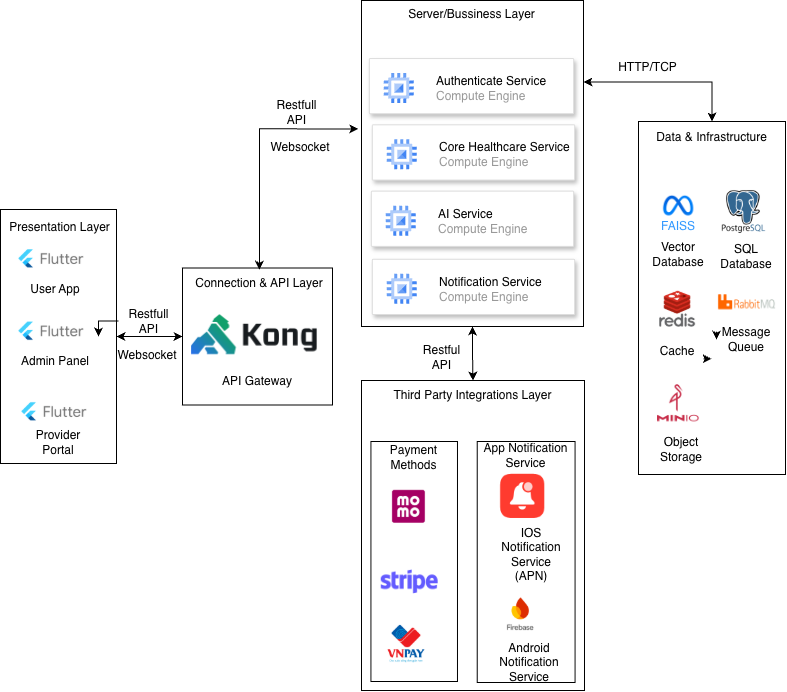
\includegraphics[width=1\textwidth]{Images/implement_arch.png}
    \vspace{10pt}
    
    % Thêm chú thích cho hình ảnh
    \caption{Kiến trúc hiện thực hệ thống}
    
    % Đặt nhãn để tham chiếu chéo (cross-reference)
    \label{fig:imple_arch}
\end{figure}

Hệ thống được thiết kế dựa trên mô hình Microservices hiện đại, chia thành 5 tầng chính với các công nghệ cụ thể như sau:

\subsection*{Tầng Giao Diện (Presentation Layer)}
Đây là tầng tương tác trực tiếp với người dùng cuối (tương ứng với Client Layer trong bản thiết kế trừu tượng).

\begin{itemize}
    \item \textbf{Công nghệ:} Flutter.
    \item \textbf{Mô tả:} Sử dụng Flutter làm công nghệ chủ đạo (Cross-platform) để xây dựng cả 3 ứng dụng client:
    \begin{itemize}
        \item \textit{User App:} Ứng dụng di động dành cho người dùng phổ thông.
        \item \textit{Admin Panel:} Trang quản trị hệ thống.
        \item \textit{Provider Portal:} Cổng thông tin dành cho các nhà cung cấp dịch vụ y tế/làm đẹp.
    \end{itemize}
    \item \textbf{Giao thức:} Các ứng dụng này giao tiếp với hệ thống backend thông qua RESTful API và WebSocket (dành cho các tính năng thời gian thực).
\end{itemize}

\subsection*{Tầng Kết Nối \& API (Connection \& API Layer)}
Đóng vai trò là cổng vào duy nhất (Entry point) cho mọi yêu cầu từ phía Client.

\begin{itemize}
    \item \textbf{Công nghệ:} Kong API Gateway.
    \item \textbf{Mô tả:} Thay thế cho khối "API Gateway" trừu tượng. Kong chịu trách nhiệm:
    \begin{itemize}
        \item Routing (định tuyến) request đến đúng microservice.
        \item Load balancing (cân bằng tải).
        \item Authentication/Authorization cơ bản (xác thực sơ bộ).
        \item Rate limiting (giới hạn băng thông) để bảo vệ hệ thống.
    \end{itemize}
\end{itemize}

\subsection*{Tầng Server \& Nghiệp Vụ (Server/Business Layer)}
Đây là lõi của hệ thống, được triển khai theo kiến trúc Microservices.

\begin{itemize}
    \item \textbf{Hạ tầng:} Compute Engine (Google Cloud Platform - GCP). Các dịch vụ được triển khai trên các máy ảo (VM) hoặc Container chạy trên VM.
    \item \textbf{Các dịch vụ thành phần:}
    \begin{itemize}
        \item \textit{Authenticate Service:} Xử lý đăng ký, đăng nhập, cấp phát token (JWT).
        \item \textit{Core Healthcare Service:} Xử lý nghiệp vụ chính như đặt lịch hẹn (Appointments), quản lý hồ sơ y tế, thanh toán.
        \item \textit{AI Service:} Chịu trách nhiệm về các tính năng thông minh (Chatbot, Recommendation System). Dịch vụ này giao tiếp chặt chẽ với Vector Database.
        \item \textit{Notification Service:} Quản lý việc gửi thông báo đẩy (Push) và Email.
    \end{itemize}
\end{itemize}

\subsection*{Tầng Dữ Liệu \& Hạ Tầng (Data \& Infrastructure Layer)}
Tầng này lưu trữ và quản lý luồng dữ liệu, cụ thể hóa các khối database trừu tượng:

\begin{itemize}
    \item \textbf{Relational Database (SQL):} Sử dụng \textbf{PostgreSQL}. Dùng để lưu trữ dữ liệu có cấu trúc (thông tin user, đơn hàng, lịch hẹn).
    \item \textbf{Vector Database:} Sử dụng \textbf{FAISS} (Facebook AI Similarity Search). Dùng để lưu trữ vector embeddings phục vụ cho AI Service (tìm kiếm ngữ nghĩa, gợi ý).
    \item \textbf{Cache:} Sử dụng \textbf{Redis}. Giúp tăng tốc độ truy xuất dữ liệu thường xuyên sử dụng và giảm tải cho Database chính.
    \item \textbf{Message Queue:} Sử dụng \textbf{RabbitMQ}. Đảm bảo giao tiếp bất đồng bộ (asynchronous) giữa các microservices (ví dụ: Core Service gửi sự kiện đến Notification Service mà không cần chờ đợi).
    \item \textbf{Object Storage:} Sử dụng \textbf{MinIO}. Giải pháp lưu trữ đối tượng (tương thích S3) dùng để lưu trữ file tĩnh, hình ảnh, tài liệu y tế (thay thế cho khối Cloud Storage trừu tượng).
\end{itemize}

\subsection*{Tầng Tích Hợp Bên Thứ Ba (Third-Party Integrations Layer)}
Kết nối với các dịch vụ bên ngoài để mở rộng tính năng.

\begin{itemize}
    \item \textbf{Cổng thanh toán (Payment Methods):} Tích hợp đa dạng bao gồm MoMo, Stripe (quốc tế), và VNPay (nội địa Việt Nam).
    \item \textbf{Dịch vụ thông báo (App Notification Service):}
    \begin{itemize}
        \item \textit{APNs (Apple Push Notification service):} Dành riêng cho thiết bị iOS.
        \item \textit{Firebase (FCM):} Dành cho Android và quản lý thông báo chung.
    \end{itemize}
\end{itemize}

\vspace{1cm} % Khoảng cách một chút trước phần nhận xét

\subsection*{Nhận xét tổng quan}
Kiến trúc này rất hiện đại và phù hợp với quy mô dự án nền tảng Health/Beauty. Việc tách biệt rõ ràng giữa PostgreSQL (nghiệp vụ) và FAISS (AI) cho thấy sự đầu tư kỹ lưỡng vào hiệu năng xử lý dữ liệu thông minh. Sử dụng MinIO cũng là một giải pháp hay để tự chủ (self-hosted) việc lưu trữ dữ liệu thay vì phụ thuộc hoàn toàn vào cloud public storage đắt đỏ.
\section{Phần Software – Triển khai ứng dụng}

Hệ thống Backend được xây dựng dựa trên \textbf{NestJS Framework}, tuân theo kiến trúc module hóa để đảm bảo tính mở rộng và bảo mật. Phần hiện thực được tổ chức theo bốn phân hệ chính dựa trên góc nhìn người dùng: (1)~Hạ tầng nền tảng dùng chung, (2)~Ứng dụng Người bệnh, (3)~Cổng Đối tác, và (4)~Trang Quản trị --- khớp với phân nhóm Use Case đã phân tích ở chương trước và kịch bản demo End-to-End trước Hội đồng.


% ===========================================================================
% 6.3.1  HẠ TẦNG NỀN TẢNG VÀ DỊCH VỤ CHUNG (CORE)
% ===========================================================================
\subsection{Hiện thực Hạ tầng nền tảng và Dịch vụ chung}

Trước khi đi vào chi tiết từng phân hệ người dùng, phần này trình bày các thành phần hạ tầng kỹ thuật dùng chung cho toàn bộ hệ thống. Đây là ``móng nhà'' mà cả ba cổng (User App, Partner Portal, Admin Portal) đều dựa trên: từ cơ chế xác thực JWT, chuẩn hóa dữ liệu DTO, quản lý tệp tin, đến hệ thống thông báo đa kênh và cầu nối với cụm AI microservices.

\subsubsection{Cấu hình và Khởi tạo hệ thống (Bootstrap \& Configuration)}

Điểm khởi chạy của ứng dụng nằm tại \texttt{src/main.ts}, nơi thiết lập các cấu hình toàn cục quan trọng cho bảo mật và tài liệu hóa API:

\begin{itemize}
    \item \textbf{Bảo mật HTTP:} Tích hợp thư viện \texttt{helmet} để thiết lập các HTTP headers an toàn và kích hoạt \texttt{enableCors()} cho phép các ứng dụng Client (Mobile/Web) truy cập tài nguyên.
    
    \item \textbf{Kiểm soát dữ liệu đầu vào:} Sử dụng \texttt{ValidationPipe} ở mức toàn cục (\texttt{globalPipes}) với tùy chọn \texttt{whitelist: true}. Điều này giúp tự động loại bỏ các trường dữ liệu thừa không được định nghĩa trong DTO.
    
    \item \textbf{Xác thực Webhook (Stripe):} Bật tùy chọn \texttt{rawBody: true} để xác thực chữ ký webhook Stripe. Khởi tạo \texttt{RedisIoAdapter} cho WebSocket scale ngang và kết nối RabbitMQ consumer với queue \texttt{checkout\_queue}.
\end{itemize}

\subsubsection{Module Thanh toán (Payment Gateway Module)}

\texttt{PaymentGatewayModule} hỗ trợ song parallel hai cổng thanh toán chính: MoMo (nội địa Việt Nam) và Stripe (quốc tế). Cấu trúc API như sau:

\begin{itemize}
    \item \textbf{Phía người dùng:} Các endpoint \texttt{POST /v1/user/payments/momo/*} và \texttt{POST /v1/user/payments/stripe/*} cho phép tạo đơn thanh toán, hoàn tiền, và kiểm tra trạng thái.
    
    \item \textbf{Phía callback:} Các endpoint công khai \texttt{POST /v1/public/momo/ipn} (Immediate Payment Notification) và \texttt{POST /v1/public/stripe/webhook} để xử lý các sự kiện từ phía gateway, theo mô hình server-to-server.
\end{itemize}

\subsubsection{Module Tích hợp AI (AI Service Integration)}

\texttt{AiServiceController} cung cấp endpoint nội bộ:

\begin{itemize}
    \item \texttt{POST /v1/ai/recommendations} - Trả về danh sách dịch vụ được gợi ý kèm thông tin đầy đủ (tên, mô tả, giá, hình ảnh, vị trí).
    
    \item Bảo vệ bằng API key header \texttt{X-AI-API-Key} để chỉ cho phép gọi machine-to-machine từ cụm AI Gateway.
\end{itemize}

\subsubsection{Cụm Microservices AI (FastAPI Services)}

Module \texttt{AuthModule} đóng vai trò trung tâm trong việc quản lý định danh, sử dụng kết hợp \textbf{Passport} và \textbf{JWT}.

\paragraph{Quy trình Đăng ký \& Đăng nhập}
\begin{itemize}
    \item \textbf{Đăng ký (\texttt{register}):} \texttt{AuthService} tiếp nhận DTO đăng ký, thực hiện băm mật khẩu (hashing) bằng thuật toán \texttt{bcrypt} trước khi lưu vào cơ sở dữ liệu. Nếu có thông tin \texttt{profile}, hệ thống sẽ khởi tạo đồng thời \texttt{Account} và \texttt{UserProfile} nhờ cơ chế \texttt{cascade: true} của TypeORM.
    
    \item \textbf{Đăng nhập (\texttt{login}):} Sử dụng \texttt{LocalStrategy} để xác thực email/password. Sau khi thành công, hệ thống cấp phát cặp token gồm \texttt{access\_token} (ngắn hạn) và \texttt{refresh\_token} (dài hạn).
\end{itemize}

\paragraph{Cơ chế Bảo mật Token (JWT Strategy)}
\begin{itemize}
    \item \textbf{Access Token:} Được ký (sign) bằng \texttt{jwtConstants.secret}. Các request đến API được bảo vệ bởi \texttt{JwtAuthGuard}, sử dụng \texttt{JwtStrategy} để trích xuất và xác thực token từ Header (\texttt{Bearer Token}).
    
    \item \textbf{Refresh Token Rotation \& Hashing:} Để tăng cường bảo mật, \texttt{refresh\_token} không được lưu trực tiếp dưới dạng plain-text. Hệ thống chỉ lưu bản băm (hash) của nó vào cột \texttt{refreshTokenHash} trong bảng \texttt{Account}. Khi user yêu cầu cấp mới token (\texttt{/auth/refresh}), hệ thống so sánh token gửi lên với hash trong DB. Điều này ngăn chặn việc sử dụng lại token cũ nếu bị lộ.
    
    \item \textbf{Logout an toàn:} API \texttt{/auth/logout} thực hiện xóa \texttt{refreshTokenHash} trong DB, đảm bảo token cũ mất hiệu lực ngay lập tức.
\end{itemize}

% TODO: Hình sơ đồ luồng JWT (login → sign → refresh rotation → hash DB → logout)

\subsubsection{Kiến trúc DTO và Validation}

Hệ thống áp dụng chặt chẽ mô hình \textbf{Data Transfer Object (DTO)} để kiểm soát dữ liệu giao tiếp:

\begin{itemize}
    \item \textbf{Validation Rules:} Sử dụng các decorator như \texttt{@IsEmail}, \texttt{@MinLength(8)} cho mật khẩu, và \texttt{@Matches} cho số điện thoại (Regex kiểm tra định dạng số Việt Nam \texttt{+84...}).
    
    \item \textbf{Nested Validation:} Hỗ trợ validate dữ liệu lồng nhau (ví dụ: object \texttt{profile} bên trong \texttt{register} request) thông qua \texttt{@ValidateNested} và \texttt{Type(() => RegisterProfileDto)}.
\end{itemize}

\subsubsection{Quản lý Tệp tin và Lưu trữ (S3 File Management)}

Module \texttt{S3Module} tích hợp với dịch vụ lưu trữ đối tượng tương thích S3 (MinIO) để quản lý tệp tin:

\begin{itemize}
    \item \textbf{Upload:} Tạo Pre-signed URL cho phép Client upload trực tiếp đến storage mà không qua Backend, giảm tải cho server.
    \item \textbf{Download:} Sinh Pre-signed URL có thời hạn để truy cập tệp tin (tài liệu doanh nghiệp, hình ảnh sản phẩm).
    \item \textbf{Quản lý tài liệu đối tác:} Thực thể \texttt{PartnerDocument} lưu metadata (loại tài liệu, URL, trạng thái) trong PostgreSQL, trong khi nội dung tệp thực tế nằm trên Object Storage.
\end{itemize}

\subsubsection{Hệ thống Thông báo đa kênh (Notification)}

Module \texttt{NotificationModule} cung cấp hệ thống thông báo đa kênh phục vụ cả ba portal, với ba controller phân quyền rõ ràng:

\begin{itemize}
    \item \textbf{WebSocket:} \texttt{NotificationGateway} đẩy thông báo tức thì (đặt lịch, tin nhắn mới, nhắc hẹn).
    \item \textbf{Push Notification (FCM):} \texttt{PushNotificationService} tích hợp Firebase Cloud Messaging qua thư viện \texttt{firebase-admin}. \texttt{UserDeviceController} quản lý đăng ký/hủy đăng ký device token.
    \item \textbf{Quản lý:} \texttt{UserNotificationController} (xem, đánh dấu đã đọc), \texttt{AdminNotificationController} (broadcast hệ thống).
    \item \textbf{Bất đồng bộ:} Sự kiện thông báo phát qua RabbitMQ từ các module nghiệp vụ (\texttt{BookingModule}, \texttt{ChatModule}), không làm chậm luồng xử lý chính.
\end{itemize}

% TODO: Hình kiến trúc Notification đa kênh (3 source → RabbitMQ → NotificationService → WS + FCM + DB)

\subsubsection{Module Tích hợp AI (\texttt{AiServiceModule})}

Cầu nối giữa Backend NestJS và cụm microservices AI (Python/FastAPI). Luồng hoạt động:

\begin{enumerate}
    \item AI Gateway gọi endpoint \texttt{/ai/recommendations} kèm danh sách \texttt{service\_id} cần làm giàu thông tin.
    \item \texttt{AiServiceService} truy vấn bảng \texttt{products} kèm quan hệ (category, media, employees) từ PostgreSQL.
    \item Kết quả ánh xạ thành \texttt{AiRecommendationsResponseDto} chứa đầy đủ thông tin (tên, mô tả, giá, hình ảnh, vị trí) để hiển thị trên ứng dụng.
\end{enumerate}

Endpoint bảo vệ bằng \texttt{AiApiKeyGuard}, chỉ service nội bộ được phép truy cập.

\subsubsection{Hạ tầng Liên kết và Cross-cutting Concerns}

\paragraph{Module RabbitMQ}

Cấu hình kết nối RabbitMQ cho giao tiếp bất đồng bộ giữa các module. Module đăng ký \texttt{ClientsModule} với giao thức AMQP, hỗ trợ TLS và virtual host riêng biệt. Sử dụng chính bởi \texttt{NotificationModule} (sự kiện thông báo) và \texttt{HealthServiceModule} (đồng bộ dữ liệu với AI Recommender).

\paragraph{Module Redis}

Cung cấp kết nối Redis cho toàn bộ ứng dụng qua \texttt{RedisService}:

\begin{itemize}
    \item \textbf{Caching:} Dữ liệu tra cứu thường xuyên (dịch vụ, banner).
    \item \textbf{Pub/Sub:} Phát sự kiện \texttt{service:created}, \texttt{service:updated}, \texttt{service:deleted} để AI Recommender đồng bộ vector store.
    \item \textbf{Distributed Locking:} Khóa phân tán cho slot đặt lịch, ngăn double-booking.
    \item \textbf{Session/TTL:} Checkout ticket, OTP, dữ liệu tạm thời.
\end{itemize}

% TODO: Hình sơ đồ Redis multi-purpose (4 blocks: Cache, Distributed Lock, Pub/Sub, Session/TTL)

\paragraph{Middleware, Interceptor và Guard}

Các cơ chế xuyên suốt (cross-cutting concerns):

\begin{itemize}
    \item \textbf{LoggingMiddleware:} Ghi method, URL, thời gian phản hồi, status code trên mọi route.
    \item \textbf{ResponseInterceptor:} Chuẩn hóa response về format \texttt{\{statusCode, message, data\}}.
    \item \textbf{PublicThrottlerGuard:} Rate limiting 100 request/60 giây cho route công khai.
    \item \textbf{WsContractBootstrapService:} Tự động đăng ký WebSocket event contracts khi khởi động.
\end{itemize}


% ===========================================================================
% 6.3.2  PHÂN HỆ ỨNG DỤNG NGƯỜI BỆNH (USER APP)
% ===========================================================================
\subsection{Hiện thực Phân hệ Ứng dụng Người bệnh (User App)}

Phân hệ này hiện thực toàn bộ trải nghiệm của người bệnh trên ứng dụng di động, từ lúc đăng ký tài khoản đến khi hoàn thành dịch vụ và đánh giá. Luồng trải nghiệm xuyên suốt bao gồm: tạo tài khoản và khảo sát sức khỏe $\rightarrow$ khám phá phòng khám/dịch vụ theo vị trí $\rightarrow$ tương tác với Chatbot AI $\rightarrow$ chọn dịch vụ vào giỏ hàng $\rightarrow$ đặt lịch với cơ chế khóa slot phân tán $\rightarrow$ thanh toán qua MoMo $\rightarrow$ đánh giá chuyên gia và dịch vụ.

\subsubsection{Đăng nhập và Đăng ký Tài khoản}

Luồng khởi tạo tài khoản của ứng dụng người bệnh được tổ chức theo mô hình tách riêng \textbf{đăng nhập} và \textbf{đăng ký}, giúp người dùng quay lại đăng nhập nhanh, đồng thời buộc người dùng mới hoàn thiện đủ thông tin định danh trước khi sử dụng các chức năng đặt lịch và thanh toán.

\begin{enumerate}
    \item \textbf{Màn hình vào cổng xác thực:} Người dùng chọn giữa hai nhánh thao tác chính là \texttt{Sign In} hoặc \texttt{Create an account}. Cách tổ chức này giảm nhầm lẫn giữa người dùng mới và người dùng đã có tài khoản.

    \item \textbf{Đăng nhập tài khoản hiện có:} Người dùng nhập email và mật khẩu, có thể sử dụng liên kết \texttt{Forgot Password?} khi quên mật khẩu. Giao diện đồng thời hỗ trợ đăng nhập nhanh bằng Google và Facebook cho các trường hợp không muốn dùng mật khẩu cục bộ.

    \item \textbf{Khởi tạo đăng ký bằng email:} Với người dùng mới, hệ thống yêu cầu nhập email trước, đồng thời hiển thị điều khoản sử dụng và chính sách riêng tư ngay ở bước đầu để ràng buộc sự đồng thuận trước khi tạo tài khoản.

    \item \textbf{Xác thực email bằng OTP:} Sau bước nhập email, người dùng nhập mã xác thực được gửi qua email để chứng minh quyền sở hữu địa chỉ đăng ký và giảm nguy cơ tạo tài khoản giả mạo.

    \item \textbf{Hoàn thiện hồ sơ đăng ký:} Sau khi xác thực OTP, người dùng tiếp tục nhập họ tên pháp lý, ngày sinh, mật khẩu, xác nhận mật khẩu và địa chỉ liên hệ. Đây là tập dữ liệu nền để tạo \texttt{Account} và \texttt{UserProfile} ban đầu.

    \item \textbf{Xác nhận và kích hoạt:} Khi người dùng nhấn \texttt{Agree \& Continue}, backend thực hiện kiểm tra hợp lệ dữ liệu, băm mật khẩu bằng \texttt{bcrypt}, lưu hồ sơ và cấp token truy cập để người dùng đi tiếp sang các bước cá nhân hóa tiếp theo.
\end{enumerate}

\begin{figure}[H]
\centering
\captionsetup[subfigure]{font=small,justification=centering}
\captionsetup{skip=6pt}
\begin{subfigure}[t]{0.48\linewidth}
    \centering
    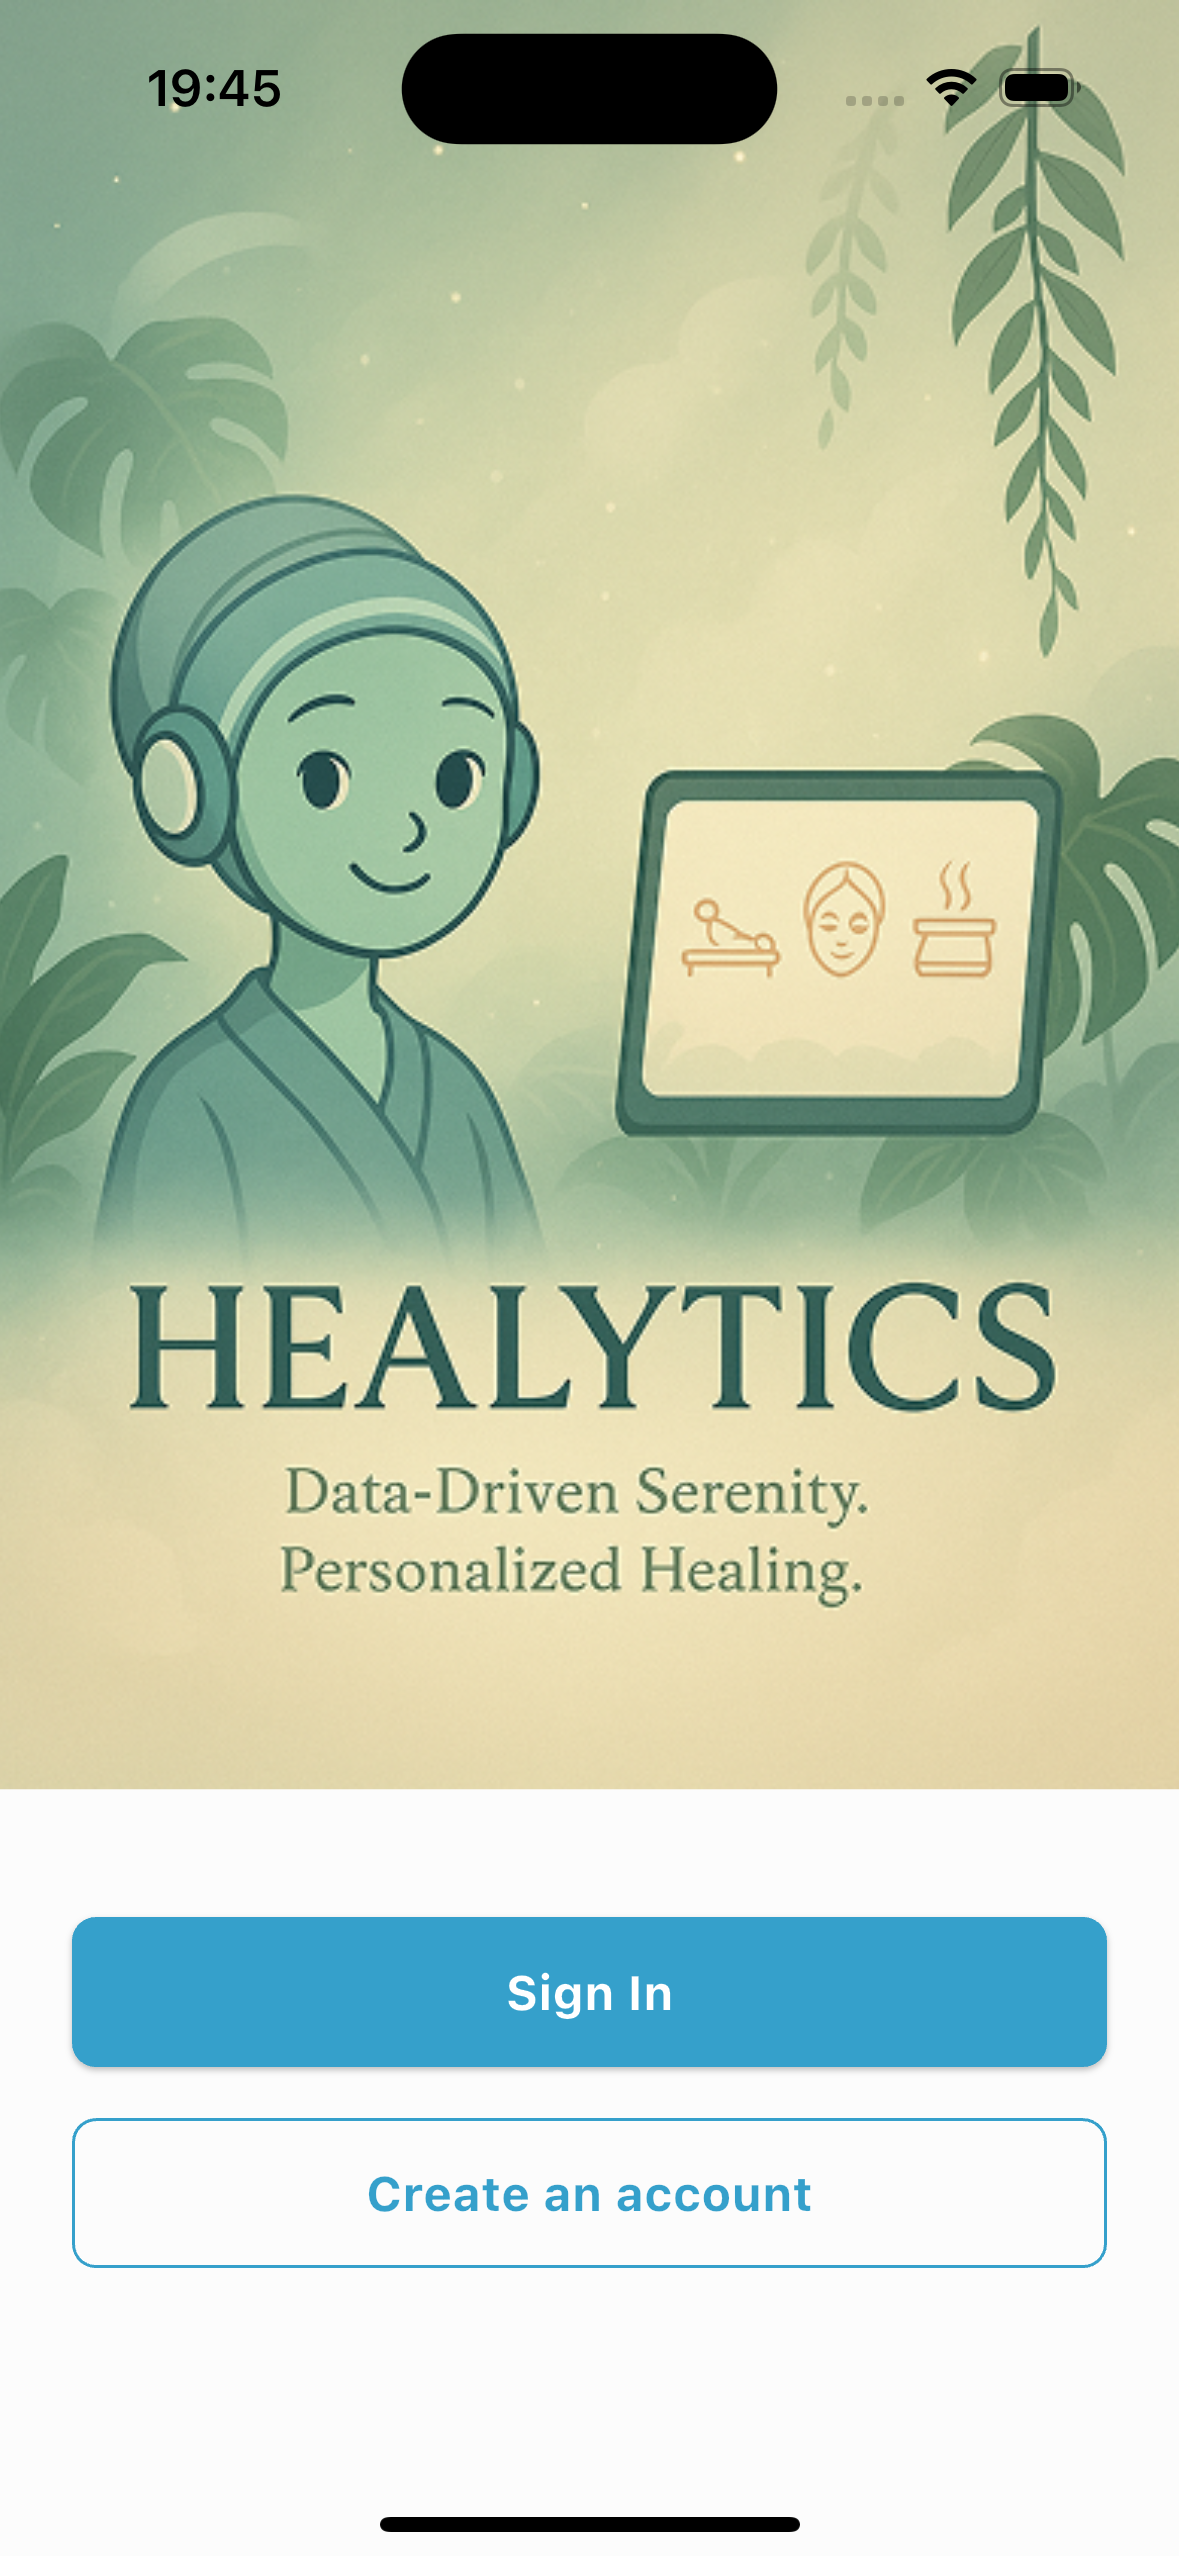
\includegraphics[width=\linewidth,height=0.4\textheight,keepaspectratio]{Images/Hiện thực/user_app/sign_in_sign_up/fig_user_auth_entry.png}
    \caption{Chọn \texttt{Sign In} hoặc \texttt{Create an account}}
    \label{fig:user_auth_entry}
\end{subfigure}
\hfill
\begin{subfigure}[t]{0.48\linewidth}
    \centering
    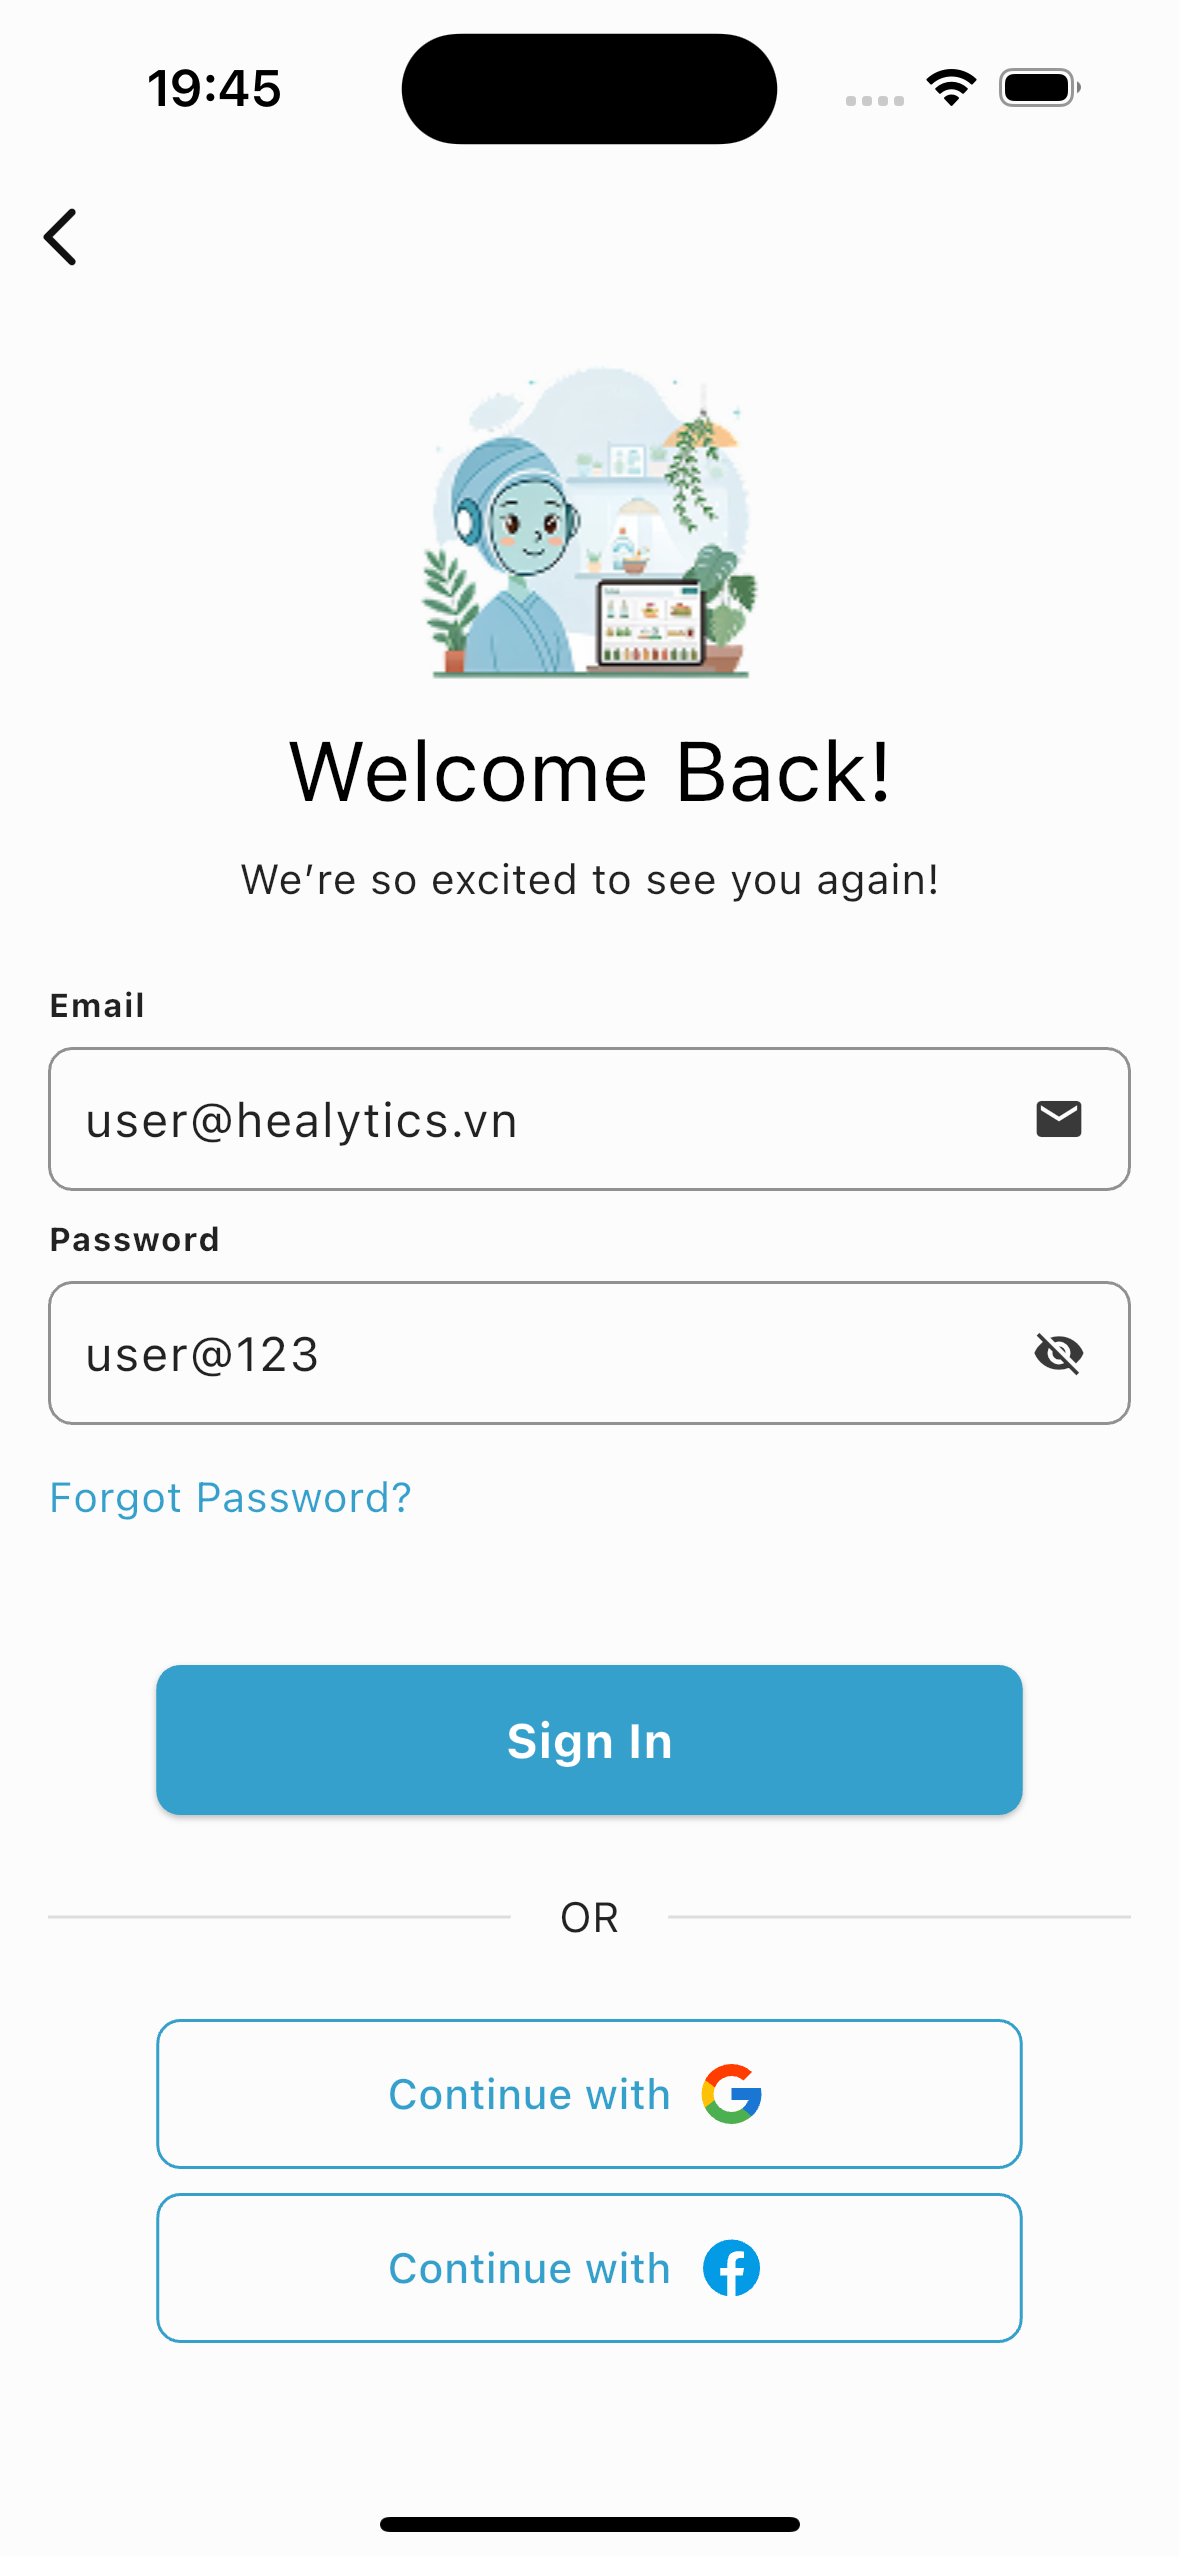
\includegraphics[width=\linewidth,height=0.4\textheight,keepaspectratio]{Images/Hiện thực/user_app/sign_in_sign_up/fig_user_auth_signin.png}
    \caption{Đăng nhập bằng email, mật khẩu hoặc social login}
    \label{fig:user_auth_signin}
\end{subfigure}
\par\medskip
\caption{Luồng Sign In của người dùng trên ứng dụng di động}
\label{fig:user_auth_signin_flow}
\end{figure}

\begin{figure}[H]
\centering
\captionsetup[subfigure]{font=small,justification=centering}
\captionsetup{skip=8pt}
\begin{subfigure}[t]{0.48\linewidth}
    \centering
    
\includegraphics[width=\linewidth,height=0.4\textheight,keepaspectratio]{Images/Hiện thực/user_app/sign_in_sign_up/fig_user_auth_email.png}
    \caption{Nhập email đăng ký}
    \label{fig:user_auth_email}
\end{subfigure}
\hfill
\begin{subfigure}[t]{0.48\linewidth}
    \centering
    
\includegraphics[width=\linewidth,height=0.4\textheight,keepaspectratio]{Images/Hiện thực/user_app/sign_in_sign_up/fig_user_auth_otp.png}
    \caption{Xác thực email bằng mã OTP}
    \label{fig:user_auth_otp}
\end{subfigure}
\par\medskip
\begin{subfigure}[t]{0.48\linewidth}
    \centering
    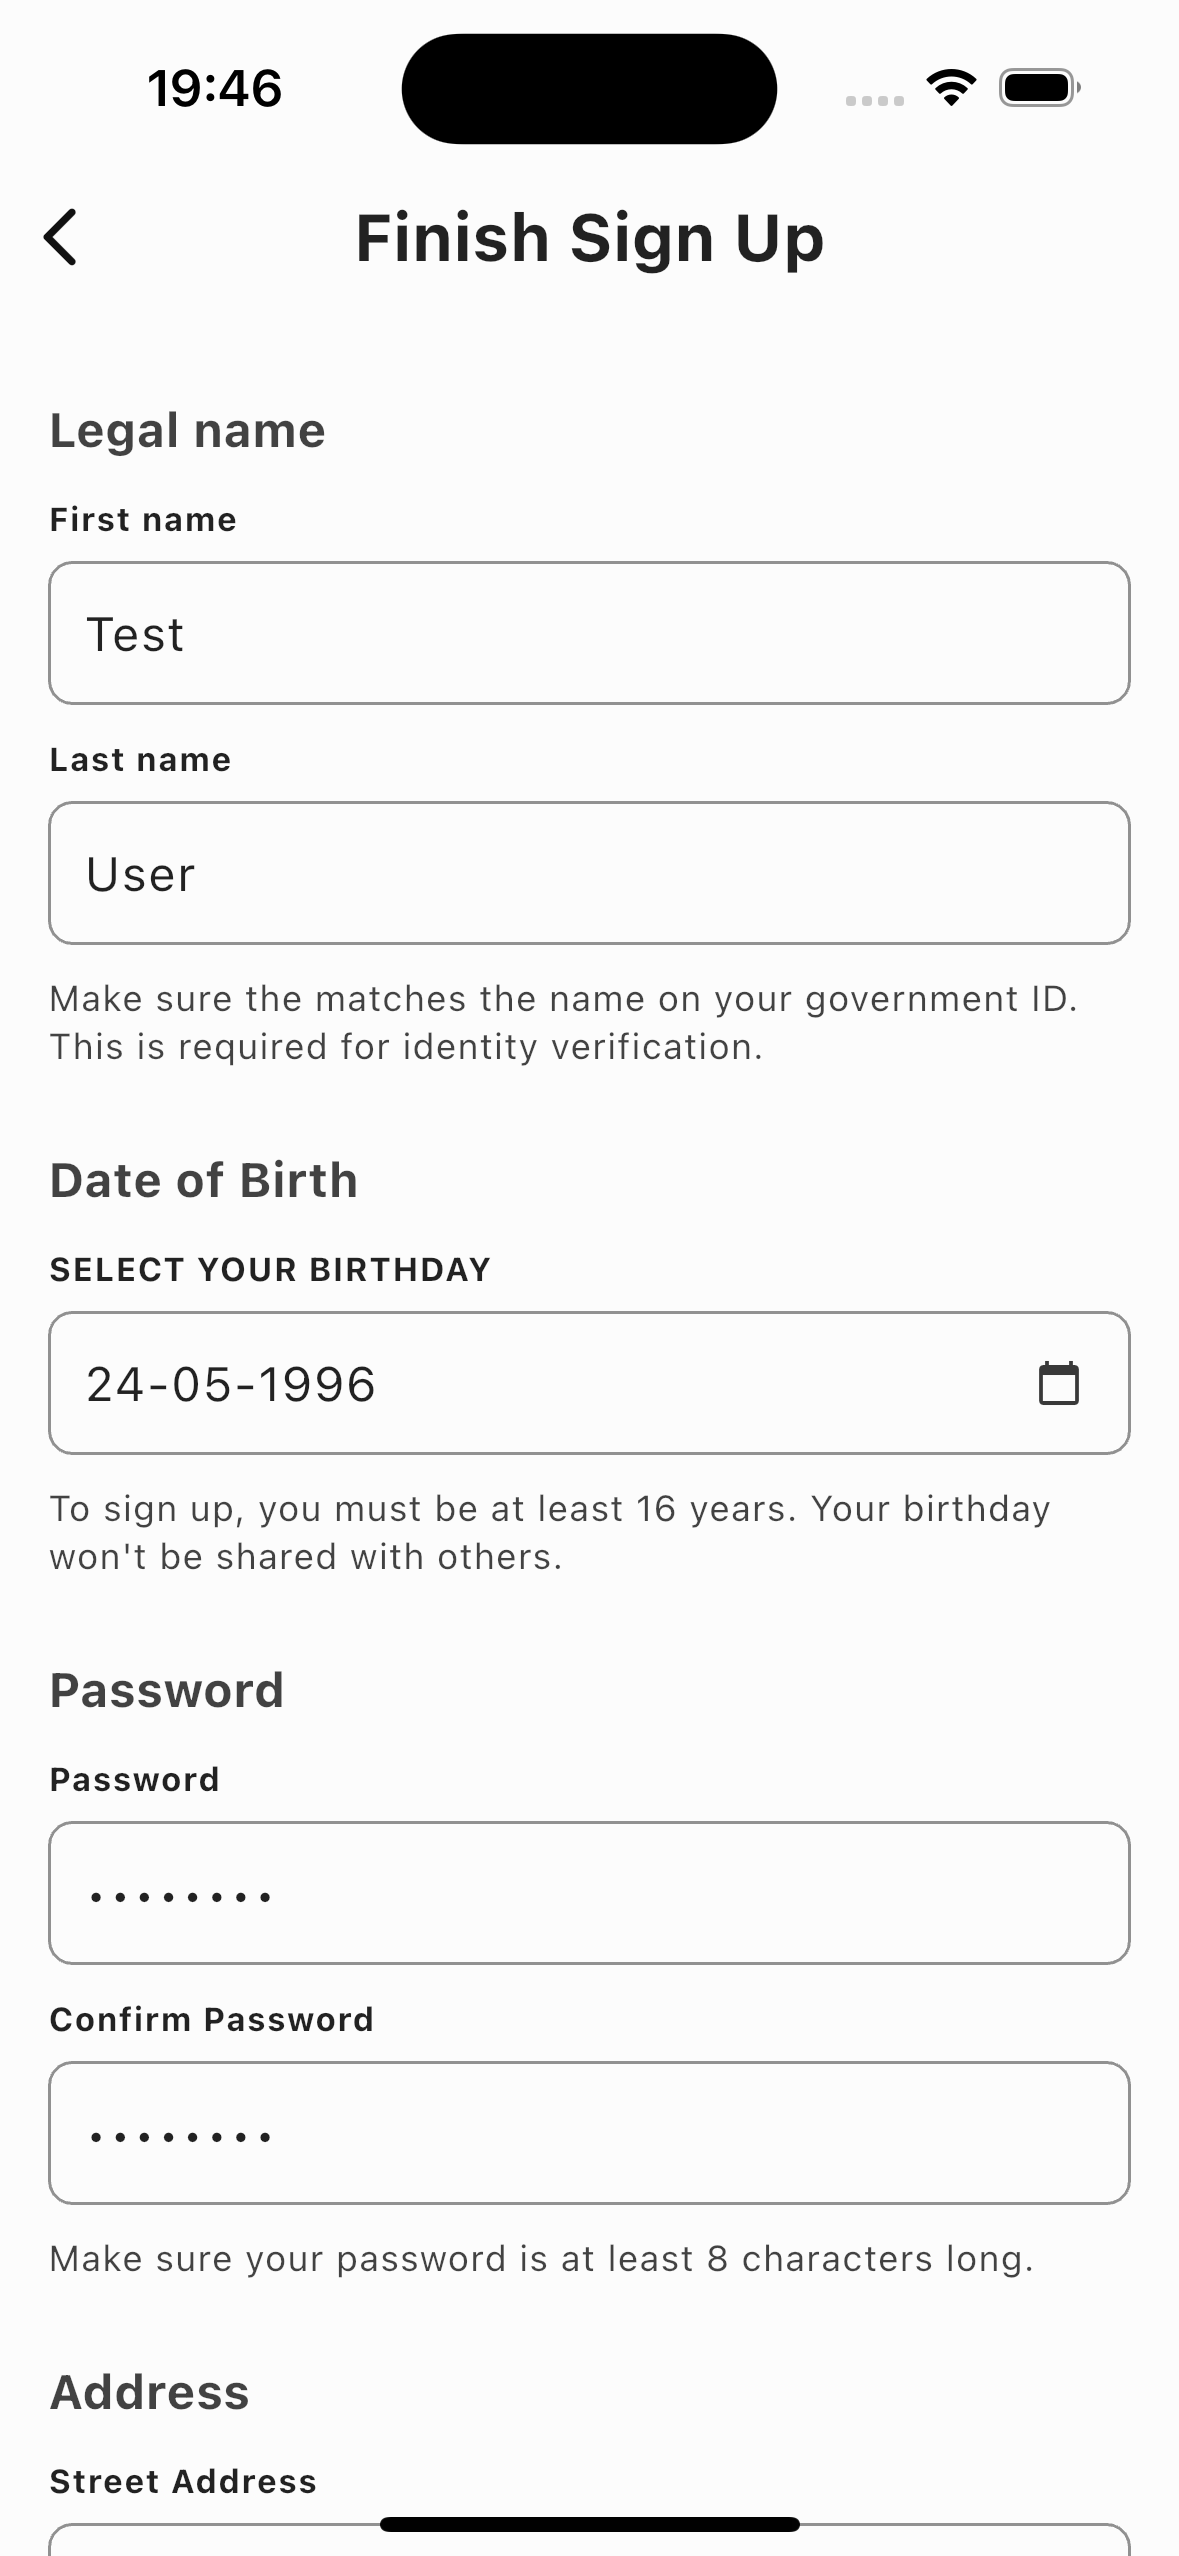
\includegraphics[width=\linewidth,height=0.4\textheight,keepaspectratio]{Images/Hiện thực/user_app/sign_in_sign_up/fig_user_auth_signup_profile.png}
    \caption{Điền thông tin cá nhân và ngày sinh}
    \label{fig:user_auth_signup_profile}
\end{subfigure}
\hfill
\begin{subfigure}[t]{0.48\linewidth}
    \centering
    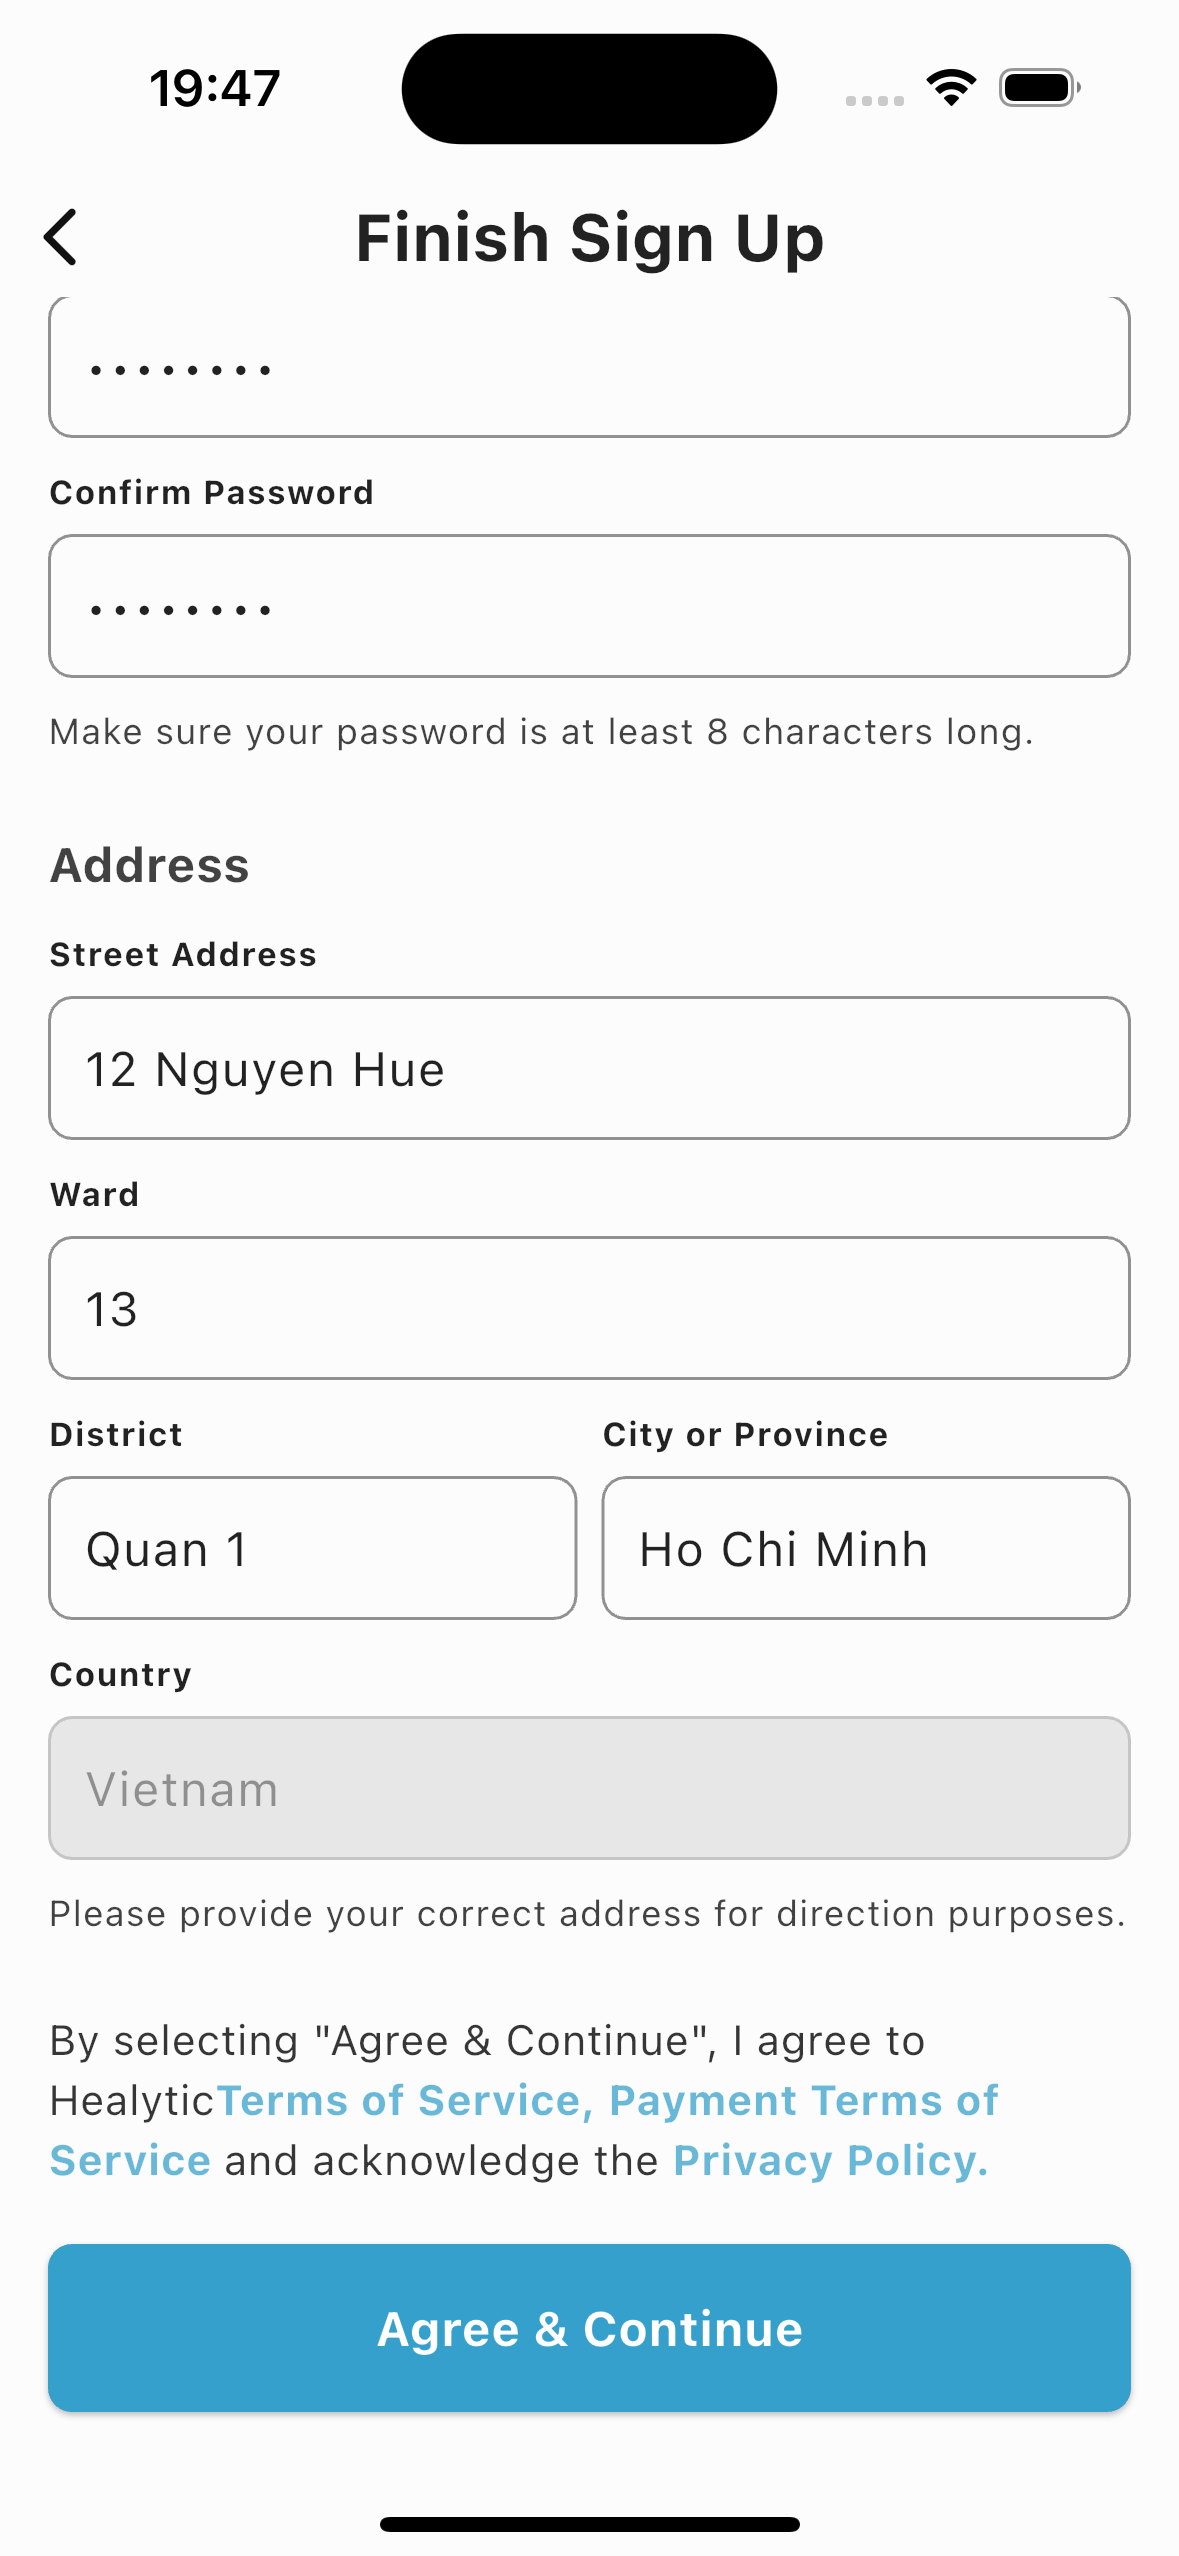
\includegraphics[width=\linewidth,height=0.4\textheight,keepaspectratio]{Images/Hiện thực/user_app/sign_in_sign_up/fig_user_auth_signup_address.png}
    \caption{Địa chỉ, điều khoản và xác nhận đăng ký}
    \label{fig:user_auth_signup_address}
\end{subfigure}
\par\medskip
\caption{Luồng Sign Up của người dùng trên ứng dụng di động}
\label{fig:user_auth_signup_flow}
\end{figure}

\paragraph{Mô tả dữ liệu và ràng buộc giao diện}

\begin{itemize}
    \item \textbf{Email:} Là định danh đăng nhập chính, được thu thập ngay từ đầu để kiểm tra định dạng và tránh trùng lặp tài khoản.
    \item \textbf{Mật khẩu:} Giao diện yêu cầu tối thiểu 8 ký tự và có trường \texttt{Confirm Password} để giảm lỗi nhập sai trước khi gửi request lên server.
    \item \textbf{Ngày sinh:} Hệ thống hiển thị ràng buộc độ tuổi tối thiểu 16 tuổi, phù hợp với yêu cầu sử dụng dịch vụ và xác minh danh tính cơ bản.
    \item \textbf{Họ tên pháp lý và địa chỉ:} Bao gồm tên thật, địa chỉ đường, phường/xã, quận/huyện, tỉnh/thành và quốc gia; đây là nhóm dữ liệu cần thiết cho nhận diện hồ sơ người dùng và các tác vụ điều hướng, đặt lịch, thanh toán.
    \item \textbf{Điều khoản sử dụng:} Trước khi hoàn tất đăng ký, người dùng phải đồng ý với \texttt{Terms of Service}, \texttt{Payment Terms of Service} và \texttt{Privacy Policy}, tạo cơ sở pháp lý cho toàn bộ giao dịch phát sinh sau đó.
\end{itemize}

\subsubsection{Khám phá Dịch vụ và Phòng khám}

\paragraph{Module Dịch vụ Sức khỏe (\texttt{HealthServiceModule})}

Module nghiệp vụ cốt lõi phía người dùng, quản lý vòng đời dịch vụ sức khỏe trên nền tảng. \texttt{UserHealthServiceController} cung cấp các endpoint:

\begin{itemize}
    \item \textbf{Tìm kiếm dịch vụ:} Hỗ trợ tìm theo từ khóa, lọc theo danh mục (\texttt{categoryId}), tags, khoảng giá (\texttt{minPrice}/\texttt{maxPrice}), và khoảng cách địa lý.
    \item \textbf{Phân trang và sắp xếp:} Hỗ trợ sort theo giá, đánh giá trung bình, lượt đặt, hoặc khoảng cách từ vị trí người dùng.
    \item \textbf{Chi tiết dịch vụ:} Trả về đầy đủ thông tin bao gồm \texttt{ProductDefinition} (thời lượng), \texttt{ProductMedia} (hình ảnh), \texttt{ProductEmployeeEligibility} (chuyên gia đủ điều kiện), và \texttt{ProductFeatureTag} (tags đặc trưng).
\end{itemize}

Mỗi dịch vụ (\texttt{Product}) liên kết với các thực thể con: \texttt{ProductMedia} (hình ảnh/video), \texttt{ProductFacilityImage} (ảnh cơ sở), \texttt{ProductTag}/\texttt{ProductFeatureTag} (tags), \texttt{ProductEmployeeEligibility} (chuyên gia đủ điều kiện), \texttt{ProductResourceRequirement} (yêu cầu thiết bị), và \texttt{DocumentRequirement} (giấy tờ cần từ phía bệnh nhân).

% \begin{figure}[H]
%     \centering
%     \begin{subfigure}[t]{0.3\textwidth}
%         \centering
%         
\includegraphics[width=\linewidth]{Images/Hiện thực/fig_user_home.png}
%         \caption{Trang chủ với banner và danh mục}
%     \end{subfigure}
%     \hfill
%     \begin{subfigure}[t]{0.3\textwidth}
%         \centering
%         \includegraphics[width=\linewidth]{Images/Hiện thực/fig_user_explore.png}
%         \caption{Khám phá dịch vụ theo vị trí}
%     \end{subfigure}
%     \hfill
%     \begin{subfigure}[t]{0.3\textwidth}
%         \centering
%         
\includegraphics[width=\linewidth]{Images/Hiện thực/fig_user_service_detail.png}
%         \caption{Chi tiết dịch vụ}
%     \end{subfigure}
%     \caption{Luồng khám phá dịch vụ và phòng khám trên ứng dụng di động}
%     \label{fig:user_explore_flow}
% \end{figure}

\paragraph{Module Phòng khám (\texttt{ClinicModule})}

Module cung cấp trang thông tin chi tiết phòng khám cho người dùng thông qua \texttt{UserClinicController}, tổ chức theo 3 tab:

\begin{itemize}
    \item \textbf{\texttt{GET /clinics/:id/info} --- Tab ``Cửa hàng'':} Thông tin tổng quan phòng khám gồm: tên, ảnh bìa, logo, gallery, chỉ số tin cậy (rating trung bình, số đánh giá, kinh nghiệm, số khách hàng), danh sách chứng chỉ (\texttt{PartnerCertification}), và top 5 chuyên gia (kèm kinh nghiệm tính từ \texttt{start\_date} hoặc \texttt{experience\_years}).

    \item \textbf{\texttt{GET /clinics/:id/products} --- Tab ``Dịch vụ'':} Danh mục dịch vụ có phân trang, lọc theo danh mục, sắp xếp (popular, latest, top\_sales, price\_asc, price\_desc), và tìm kiếm theo tên. Mỗi dịch vụ hiển thị giá gốc, giá khuyến mãi, thời lượng, và số lượt đặt.

    \item \textbf{\texttt{GET /clinics/:id/reviews} --- Tab ``Đánh giá'':} Đánh giá phân trang, lọc theo số sao (\texttt{starCount}) hoặc chỉ hiển thị đánh giá có ảnh (\texttt{hasMedia}).
\end{itemize}

\begin{figure}[H]
\centering
\captionsetup[subfigure]{font=small,justification=centering}
\captionsetup{skip=6pt}
\begin{subfigure}[t]{0.48\linewidth}
    \centering
    
\includegraphics[width=\linewidth,height=0.38\textheight,keepaspectratio]{Images/Hiện thực/user_app/clinic_info/fig_clinic_info_1.png}
    \caption{Tab Cửa hàng -- phần tổng quan}
    \label{fig:clinic_info_overview}
\end{subfigure}
\hfill
\begin{subfigure}[t]{0.48\linewidth}
    \centering
    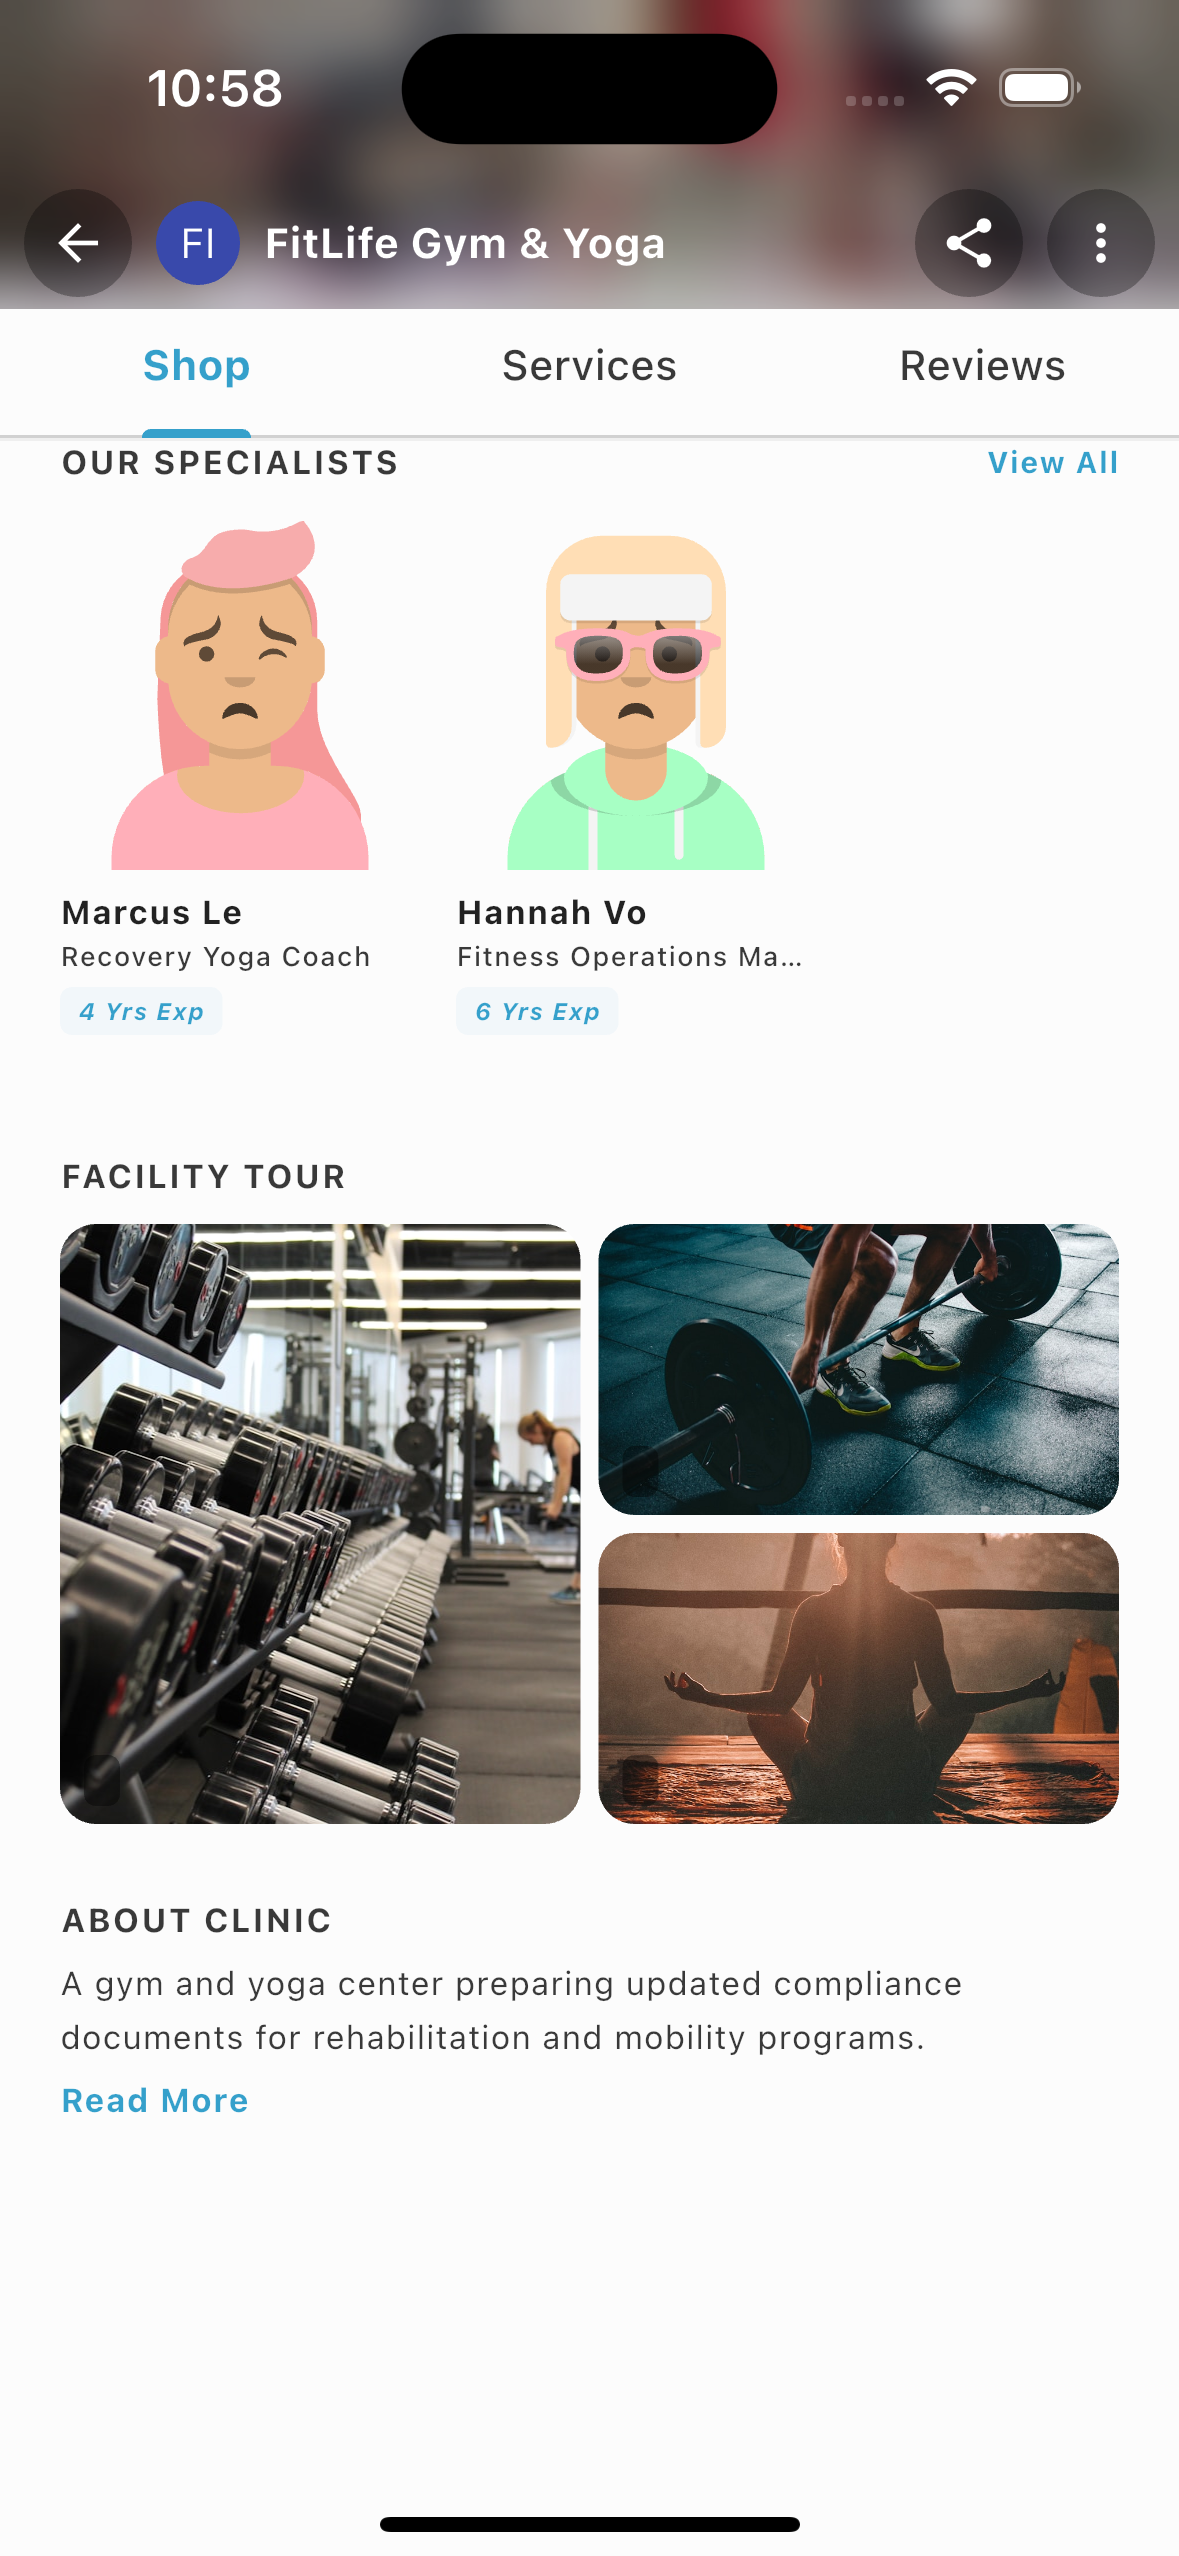
\includegraphics[width=\linewidth,height=0.38\textheight,keepaspectratio]{Images/Hiện thực/user_app/clinic_info/fig_clinic_info_2.png}
    \caption{Tab Cửa hàng -- cơ sở vật chất}
    \label{fig:clinic_info_facility}
\end{subfigure}
\par\medskip
\begin{subfigure}[t]{0.48\linewidth}
    \centering
    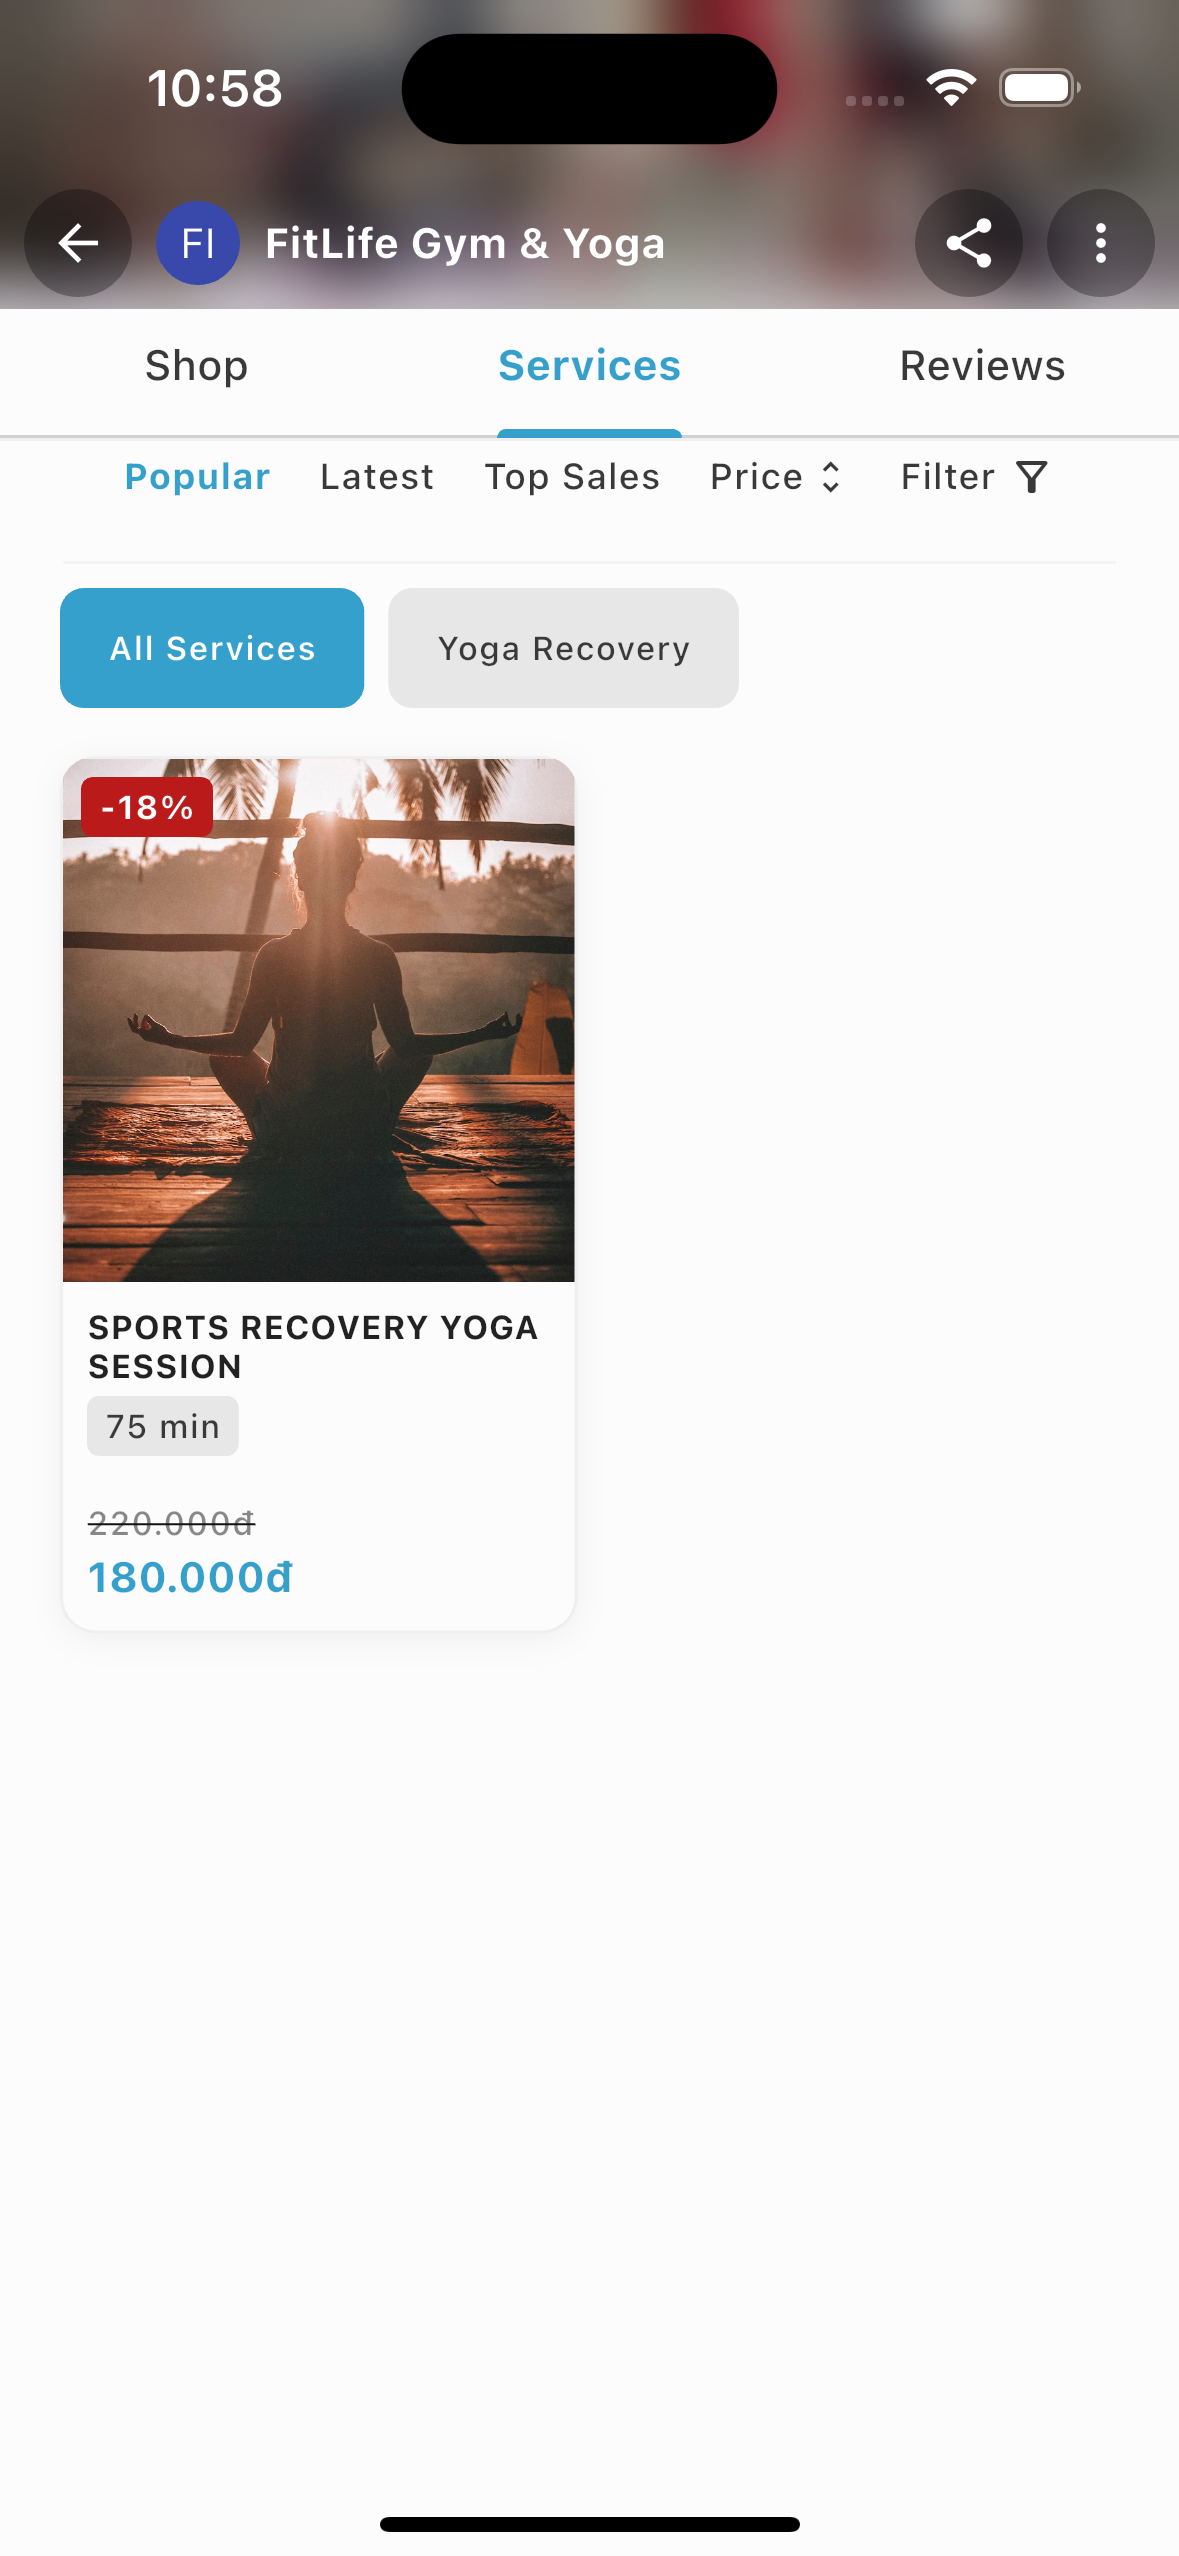
\includegraphics[width=\linewidth,height=0.38\textheight,keepaspectratio]{Images/Hiện thực/user_app/clinic_info/fig_clinic_info_3.png}
    \caption{Tab Dịch vụ -- danh sách dịch vụ}
    \label{fig:clinic_info_services}
\end{subfigure}
\hfill
\begin{subfigure}[t]{0.48\linewidth}
    \centering
    
\includegraphics[width=\linewidth,height=0.38\textheight,keepaspectratio]{Images/Hiện thực/user_app/clinic_info/fig_clinic_info_4.png}
    \caption{Tab Đánh giá}
    \label{fig:clinic_info_reviews}
\end{subfigure}
\par\medskip
\caption{Trang chi tiết phòng khám với 3 tab: Cửa hàng, Dịch vụ, Đánh giá}
\label{fig:user_clinic_detail}
\end{figure}

\paragraph{Module Danh mục (\texttt{CategoriesModule})}

Tổ chức danh mục theo cấu trúc phân cấp parent-child (ví dụ: Y tế $\rightarrow$ Tim mạch $\rightarrow$ Khám tổng quát). \texttt{CategoriesController} cung cấp API công khai (không yêu cầu xác thực), trả danh sách kèm cấu trúc cây phục vụ hiển thị menu đa cấp trên ứng dụng.

\paragraph{Module Tags dịch vụ (\texttt{ServiceTagsModule})}

Quản lý hệ thống tags gắn với dịch vụ (\textit{yoga}, \textit{giảm cân}, \textit{tim mạch}). Quan hệ many-to-many với \texttt{Product}, hỗ trợ tìm kiếm đa chiều. API cho phép lọc dịch vụ theo tổ hợp tags.

\subsubsection{Tìm kiếm theo Vị trí}

\paragraph{Module Địa chỉ hành chính (\texttt{LocationsModule})}

Quản lý hệ thống địa chỉ phân cấp theo chuẩn hành chính Việt Nam: Tỉnh/Thành phố $\rightarrow$ Quận/Huyện $\rightarrow$ Phường/Xã (\texttt{LocationLevel} enum). Phục vụ validation địa chỉ khi đăng ký đối tác, tạo phòng khám và lưu địa chỉ người dùng.

\paragraph{Module Bản đồ (\texttt{MapboxModule})}

Tích hợp Mapbox API: Geocoding (địa chỉ $\leftrightarrow$ tọa độ), tìm kiếm theo vị trí với bán kính tùy chỉnh, và tính khoảng cách giữa hai điểm phục vụ sắp xếp kết quả.

\subsubsection{Chat thời gian thực (phía Người dùng)}

Nhắn tin thời gian thực giữa người dùng và đối tác, kết hợp REST API và WebSocket:

\begin{itemize}
    \item \textbf{Kiến trúc:} \texttt{UserChatController} (REST) + \texttt{UserChatGateway} (WebSocket).
    \item \textbf{Xác thực WebSocket:} Middleware \texttt{ws-jwt-auth} xác thực JWT khi thiết lập kết nối.
    \item \textbf{Dữ liệu:} \texttt{Conversation}/\texttt{ChatMessage} (nội dung, thời gian, trạng thái đã đọc).
    \item \textbf{REST bổ trợ:} Lịch sử tin nhắn (phân trang), danh sách cuộc trò chuyện, đánh dấu đã đọc.
\end{itemize}

% Placeholder: Uncomment khi có ảnh chụp màn hình chat
% \begin{figure}[H]
%     \centering
%     \begin{subfigure}[t]{0.3\textwidth}
%         \centering
%         \includegraphics[width=\linewidth]{Images/Hiện thực/fig_user_chat_list.png}
%         \caption{Danh sách cuộc trò chuyện}
%     \end{subfigure}
%     \hfill
%     \begin{subfigure}[t]{0.3\textwidth}
%         \centering
%         \includegraphics[width=\linewidth]{Images/Hiện thực/fig_user_chat_box.png}
%         \caption{Chat với đối tác}
%     \end{subfigure}
%     \hfill
%     \begin{subfigure}[t]{0.3\textwidth}
%         \centering
%         \includegraphics[width=\linewidth]{Images/Hiện thực/fig_user_ai_chat.png}
%         \caption{Chat với AI Chatbot}
%     \end{subfigure}
%     \caption{Giao diện Chat thời gian thực và tương tác với AI Chatbot}
%     \label{fig:user_chat_flow}
% \end{figure}

\subsubsection{Đánh giá dịch vụ (\texttt{ReviewModule})}

Phân hệ đánh giá cho phép người dùng để lại nhận xét và điểm số sau khi trải nghiệm dịch vụ. Quy trình được thiết kế theo dạng từng bước (step-by-step) nhằm tối ưu tỷ lệ hoàn thành khảo sát. Hệ thống thu thập hai luồng dữ liệu chính: \texttt{SpecialistReview} (đánh giá chuyên gia về chuyên môn, thái độ) và \texttt{TreatmentReview} (đánh giá trải nghiệm điều trị, không gian, kèm ảnh chụp thực tế qua \texttt{photo\_urls} jsonb). Điểm trung bình được tổng hợp và hiển thị trực tiếp trên trang chi tiết phòng khám.

\begin{enumerate}
    \item \textbf{Đánh giá dịch vụ:} Người dùng chấm điểm mức độ hài lòng về dịch vụ tổng thể.
    \item \textbf{Đánh giá chuyên gia \& cơ sở:} Hệ thống yêu cầu đánh giá chi tiết cho chuyên gia phụ trách và cơ sở vật chất.
    \item \textbf{Nhận xét và hình ảnh:} Người dùng nhập bình luận và có thể tải lên hình ảnh đính kèm (ảnh sau điều trị, hóa đơn).
    \item \textbf{Hoàn tất:} Sau khi gửi, hệ thống ghi nhận đánh giá và hiển thị màn hình thông báo thành công.
\end{enumerate}

\begin{figure}[H]
\centering
\captionsetup[subfigure]{font=small,justification=centering}
\captionsetup{skip=8pt}
\begin{subfigure}[t]{0.48\linewidth}
    \centering
    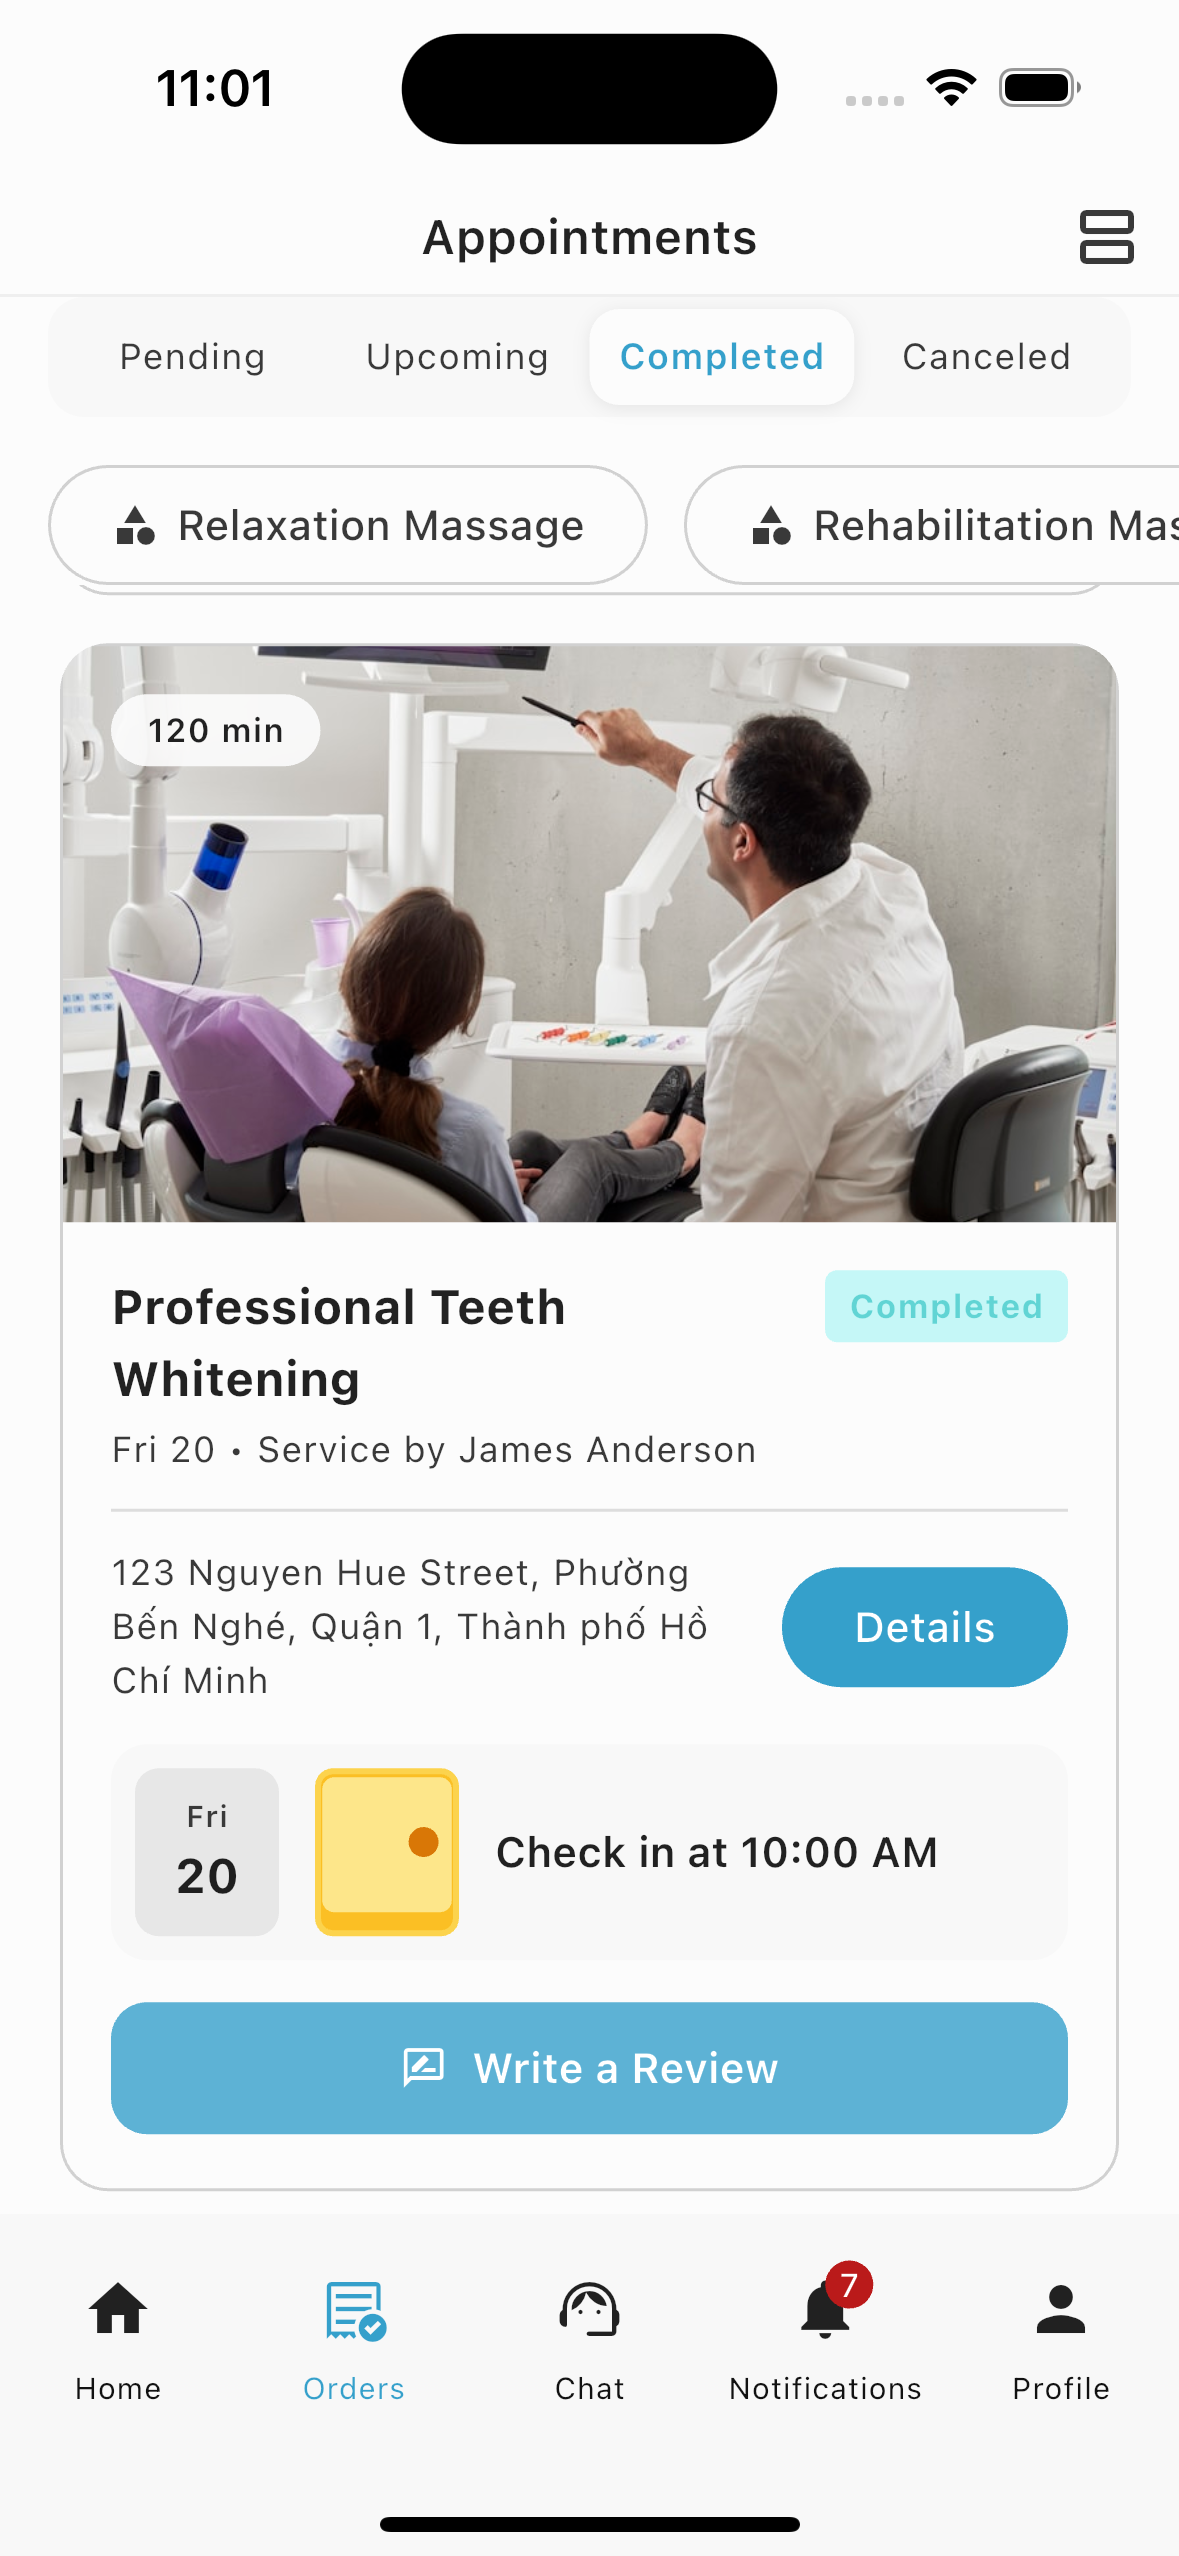
\includegraphics[width=\linewidth,height=0.35\textheight,keepaspectratio]{Images/Hiện thực/user_app/reviews/fig_review_step1.png}
    \caption{Bắt đầu đánh giá dịch vụ}
    \label{fig:review_step1}
\end{subfigure}
\hfill
\begin{subfigure}[t]{0.48\linewidth}
    \centering
    
\includegraphics[width=\linewidth,height=0.35\textheight,keepaspectratio]{Images/Hiện thực/user_app/reviews/fig_review_step2.png}
    \caption{Đánh giá chuyên gia}
    \label{fig:review_step2}
\end{subfigure}
\par\medskip
\begin{subfigure}[t]{0.48\linewidth}
    \centering
    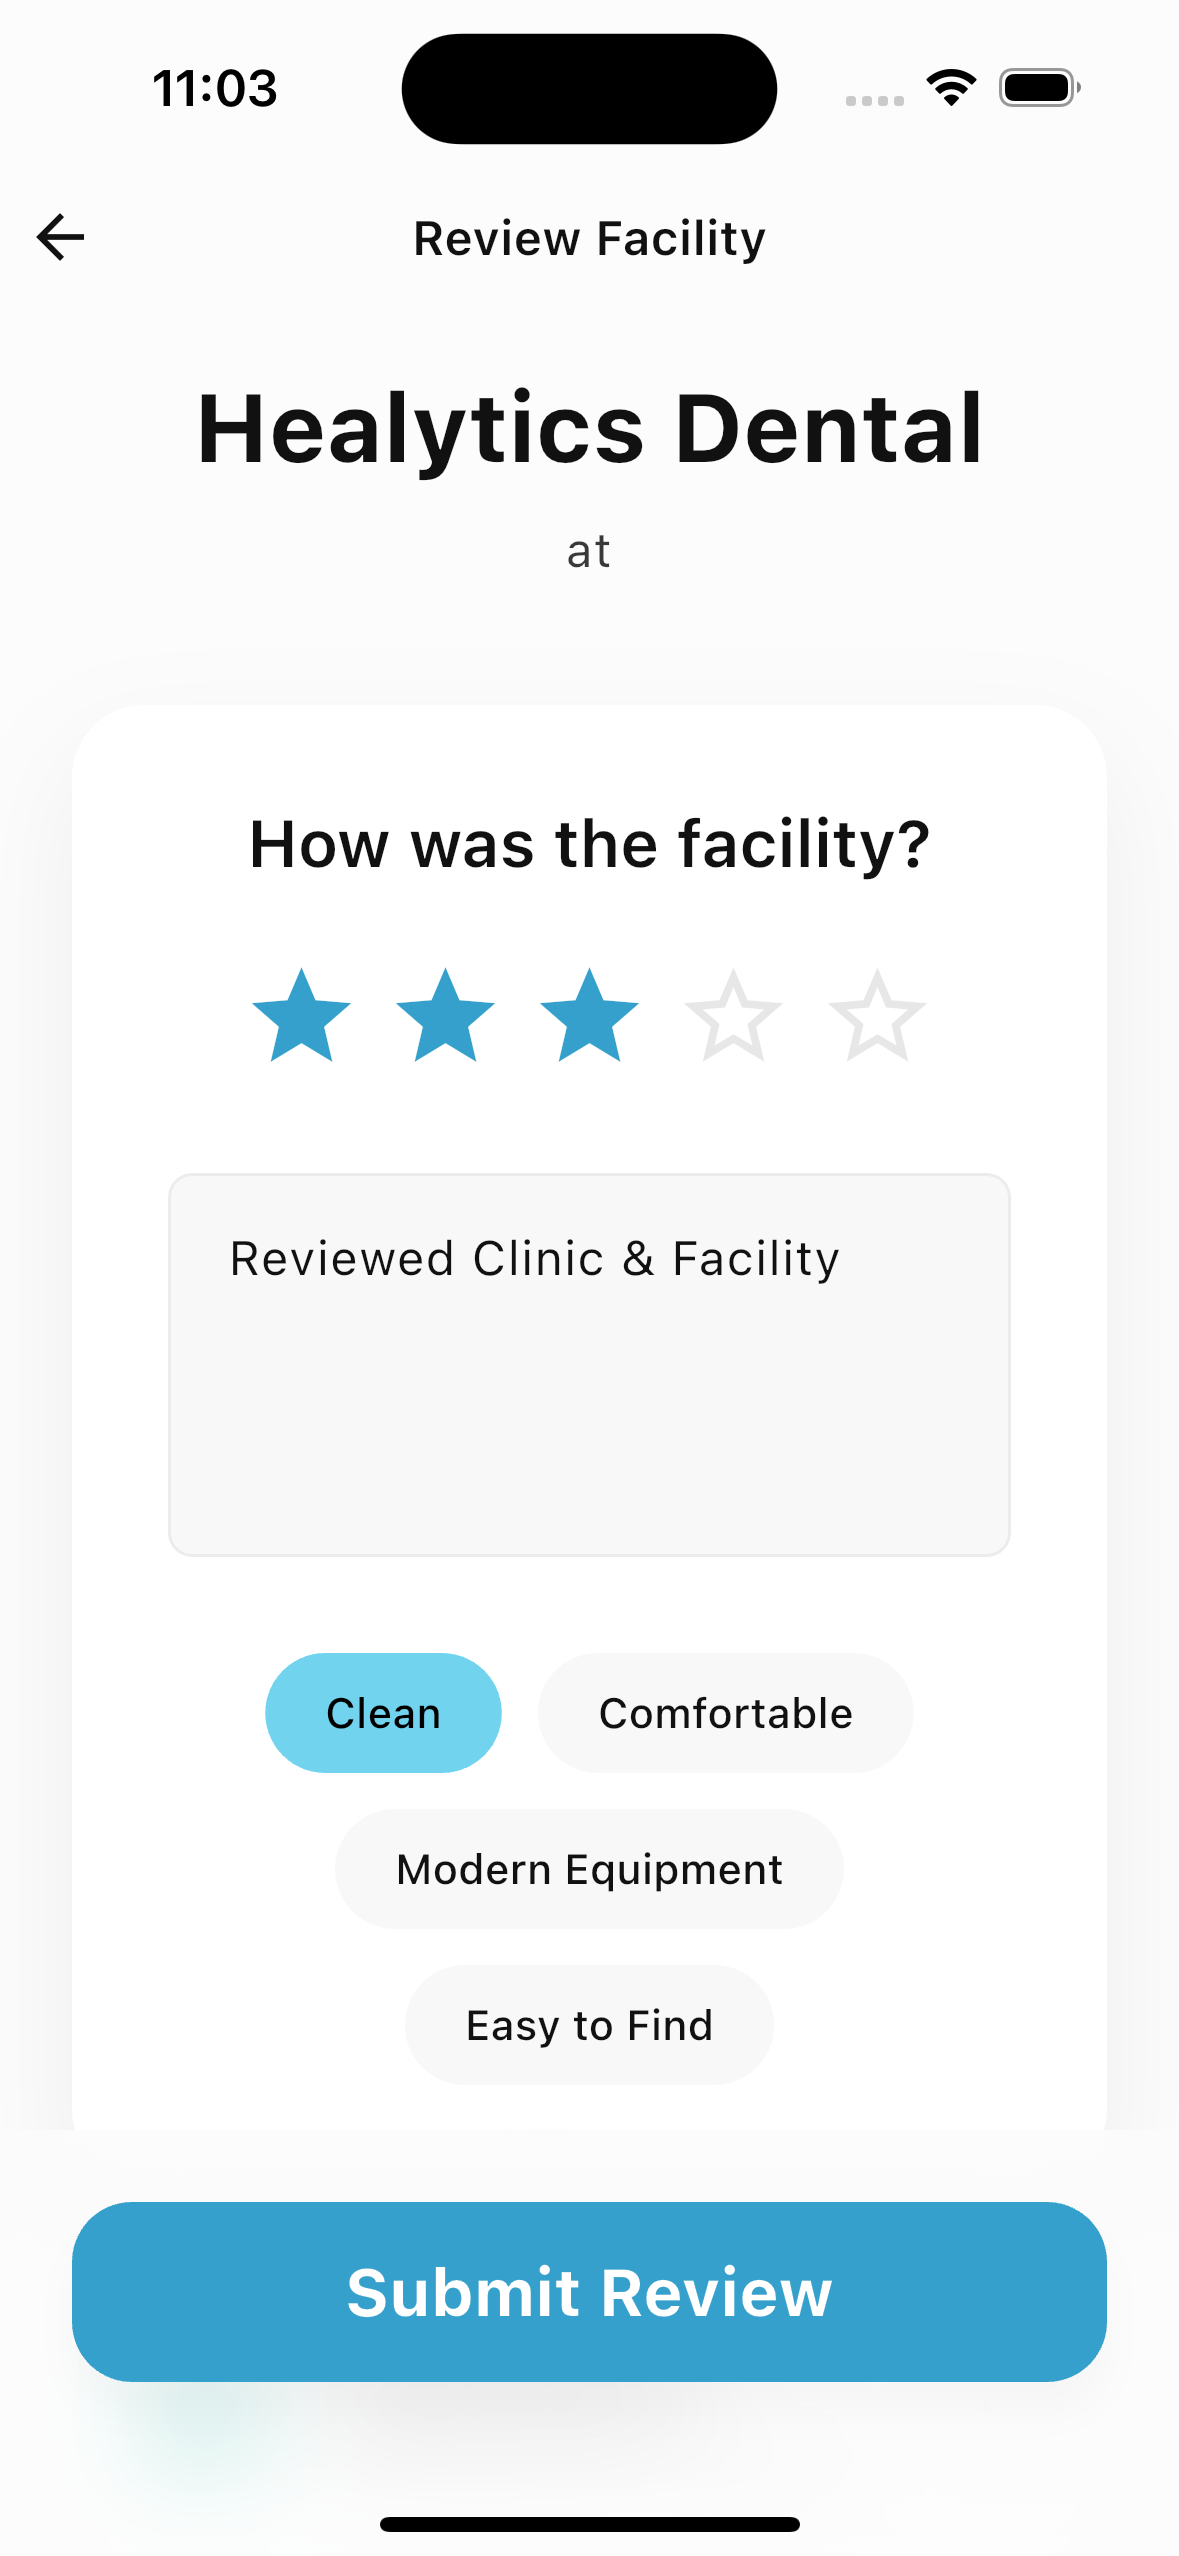
\includegraphics[width=\linewidth,height=0.35\textheight,keepaspectratio]{Images/Hiện thực/user_app/reviews/fig_review_step3.png}
    \caption{Nhận xét chi tiết và đính kèm ảnh}
    \label{fig:review_step3}
\end{subfigure}
\hfill
\begin{subfigure}[t]{0.48\linewidth}
    \centering
    
\includegraphics[width=\linewidth,height=0.35\textheight,keepaspectratio]{Images/Hiện thực/user_app/reviews/fig_review_step4.png}
    \caption{Hoàn tất đánh giá}
    \label{fig:review_step4}
\end{subfigure}
\par\medskip
\caption{Luồng Đánh giá dịch vụ (Service Review) trên ứng dụng người bệnh}
\label{fig:user_review_flow}
\end{figure}

\subsubsection{Quản lý Đặt lịch, Giỏ hàng và Thanh toán}

\paragraph{Module Đặt lịch (\texttt{BookingModule})}

Xử lý quy trình đặt lịch theo mô hình máy trạng thái:

\begin{itemize}
    \item \textbf{Luồng trạng thái:} \texttt{PENDING\_PAYMENT} $\rightarrow$ \texttt{CONFIRMED} $\rightarrow$ \texttt{IN\_PROGRESS} $\rightarrow$ \texttt{COMPLETED} hoặc \texttt{CANCELLED}. Mỗi chuyển trạng thái được ghi vào \texttt{BookingStatusLog} kèm actor, lý do, và timestamp.
    \item \textbf{Quản lý slot:} \texttt{SlotsController} kiểm tra khung giờ trống, ngăn double-booking qua khóa phân tán Redis.
    \item \textbf{Tích hợp thanh toán:} Booking xác nhận tự động kích hoạt thanh toán qua \texttt{BookingPaymentService}.
\end{itemize}

% Placeholder: Uncomment khi có ảnh chụp màn hình đặt lịch
\subsubsection{Kiến trúc giao diện User Portal}

\paragraph{Màn hình chính (Home)}

Màn hình chính là điểm khởi đầu của người dùng, cung cấp truy cập nhanh đến các tính năng chính:

\begin{figure}[H]
\centering
\captionsetup[subfigure]{font=small,justification=centering}
\captionsetup{skip=6pt}
\begin{subfigure}[t]{0.48\linewidth}
    \centering
    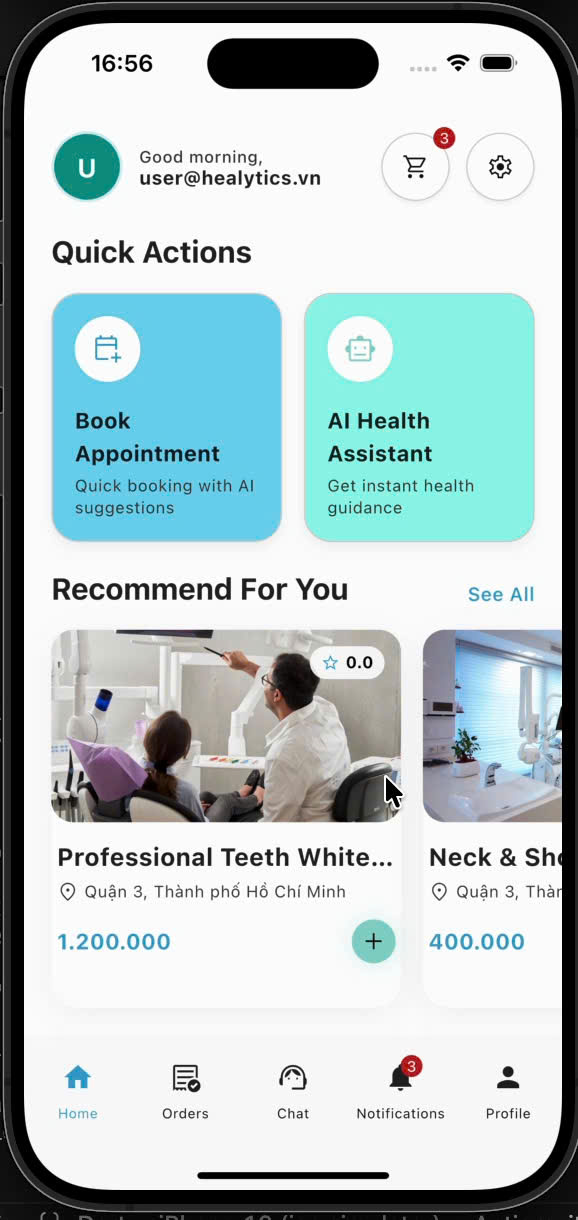
\includegraphics[width=\linewidth,height=0.4\textheight,keepaspectratio]{Images/Hiện thực/user/fig_user_home.jpg}
    \caption{Giao diện chế độ sáng với Quick Actions và Recommend For You}
    \label{fig:user_home_home}
\end{subfigure}
\hfill
\begin{subfigure}[t]{0.48\linewidth}
    \centering
    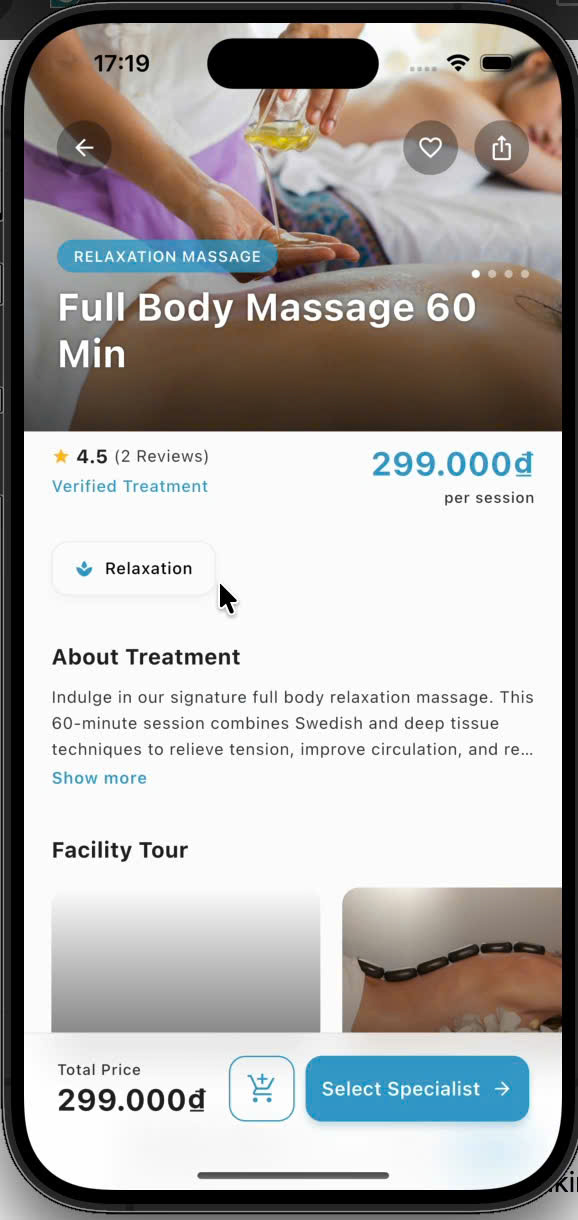
\includegraphics[width=\linewidth,height=0.4\textheight,keepaspectratio]{Images/Hiện thực/user/fig_user_service_detail.jpg}
    \caption{Chi tiết dịch vụ được đề xuất}
    \label{fig:user_home_service_detail}
\end{subfigure}
\par\medskip
\caption{Màn hình Home - Trung tâm của User Portal}
\label{fig:user_home}
\end{figure}

\begin{itemize}
    \item \textbf{Thao tác chính:} Người dùng chọn nhanh \textit{Book Appointment} hoặc \textit{AI Health Assistant} từ khối Quick Actions.
    \item \textbf{Thao tác điều hướng:} Nhấn các tab ở thanh dưới để chuyển giữa Home, Orders, Chat, Notifications và Profile.
\end{itemize}

\textbf{Thành phần chính:}

\begin{itemize}
    \item \textbf{User Profile Header:} Hiển thị tên người dùng, icon settings, và giỏ hàng.
    \item \textbf{Quick Actions:} Book Appointment và AI Health Assistant.
    \item \textbf{Recommend For You:} Carousel dịch vụ được khuyến nghị.
    \item \textbf{Bottom Navigation:} 5 tab: Home, Orders, Chat, Notifications, Profile.
\end{itemize}

\textbf{Tính năng kỹ thuật:}

\begin{itemize}
    \item \textbf{State Management:} BLoC pattern cho danh sách recommended.
    \item \textbf{Caching:} Tránh reload không cần thiết.
    \item \textbf{Pull-to-Refresh:} Làm mới danh sách dịch vụ.
\end{itemize}

\paragraph{Quản lý lịch hẹn (Appointments)}

Màn hình Appointments cho phép người dùng theo dõi toàn bộ lịch sử hẹn được phân loại thành bốn tab: Pending (chờ thanh toán), Upcoming (sắp tới), Completed (hoàn thành), và Canceled (đã hủy). Mỗi lịch hẹn được hiển thị dưới dạng card chứa thông tin dịch vụ, cơ sở y tế, chuyên gia, thời gian check-in, và trạng thái thanh toán. Người dùng có thể nhấn nút \textit{Details} để xem chi tiết đầy đủ hoặc thực hiện các hành động bổ sung.

\begin{figure}[H]
\centering
\captionsetup[subfigure]{font=small,justification=centering}
\captionsetup{skip=6pt}
\begin{subfigure}[t]{0.48\linewidth}
    \centering
    \includegraphics[width=\linewidth,height=0.36\textheight,keepaspectratio]{Images/Hiện thực/user_app/appoinment/fig_appointment_pending.png}
    \caption{Tab Pending -- chờ thanh toán}
    \label{fig:appointment_pending}
\end{subfigure}
\hfill
\begin{subfigure}[t]{0.48\linewidth}
    \centering
    \includegraphics[width=\linewidth,height=0.36\textheight,keepaspectratio]{Images/Hiện thực/user_app/appoinment/fig_appointment_upcoming.png}
    \caption{Tab Upcoming -- lịch hẹn sắp tới}
    \label{fig:appointment_upcoming}
\end{subfigure}
\par\medskip
\caption{Quản lý lịch hẹn -- danh sách hẹn theo trạng thái}
\label{fig:appointments_list}
\end{figure}

\textbf{Tính năng kỹ thuật:}

\begin{itemize}
    \item \textbf{Phân loại theo trạng thái:} Bốn tab (Pending, Upcoming, Completed, Canceled) với lazy loading 10 item/batch.
    \item \textbf{Real-time Status Sync:} WebSocket cập nhật trạng thái lịch hẹn khi có thay đổi từ phía partner.
    \item \textbf{Push Notification:} Nhắc nhở 1 giờ trước lịch hẹn qua FCM.
\end{itemize}

\paragraph{Xem chi tiết lịch hẹn và Hướng dẫn dịch vụ}

Khi người dùng nhấn nút \textit{Details} từ danh sách hẹn, màn hình Appointment Details hiển thị thông tin đầy đủ về lịch hẹn: hình ảnh dịch vụ, tên dịch vụ, cơ sở y tế, chuyên gia phụ trách, thời gian check-in/check-out, và các tùy chọn liên quan (xem hướng dẫn dịch vụ, nhắn tin với cơ sở). Người dùng có thể nhấn \textit{Service manual} để truy cập hướng dẫn chi tiết về dịch vụ, bao gồm: guidelines trước dịch vụ (Pre-Service Guidelines), các bước thực hiện dịch vụ, hình ảnh cơ sở vật chất (Facilities), và lịch sử đánh giá về dịch vụ đó. Tính năng này giúp người dùng chuẩn bị tốt trước cuộc hẹn và giao tiếp trực tiếp với nhân viên qua chat.

\begin{figure}[H]
\centering
\captionsetup[subfigure]{font=small,justification=centering}
\captionsetup{skip=6pt}
\begin{subfigure}[t]{0.48\linewidth}
    \centering
    \includegraphics[width=\linewidth,height=0.36\textheight,keepaspectratio]{Images/Hiện thực/user_app/appoinment/fig_appointment_details.png}
    \caption{Chi tiết lịch hẹn}
    \label{fig:appointment_details}
\end{subfigure}
\hfill
\begin{subfigure}[t]{0.48\linewidth}
    \centering
    \includegraphics[width=\linewidth,height=0.36\textheight,keepaspectratio]{Images/Hiện thực/user_app/appoinment/fig_appointment_manual_1.png}
    \caption{Hướng dẫn dịch vụ -- phần 1}
    \label{fig:appointment_manual_part1}
\end{subfigure}
\par\medskip
\begin{subfigure}[t]{0.48\linewidth}
    \centering
    \includegraphics[width=\linewidth,height=0.36\textheight,keepaspectratio]{Images/Hiện thực/user_app/appoinment/fig_appointment_manual_2.png}
    \caption{Hướng dẫn dịch vụ -- phần 2}
    \label{fig:appointment_manual_part2}
\end{subfigure}
\hfill
\begin{subfigure}[t]{0.48\linewidth}
    \centering
    \includegraphics[width=\linewidth,height=0.36\textheight,keepaspectratio]{Images/Hiện thực/user_app/appoinment/fig_appointment_chat.png}
    \caption{Chat với cơ sở y tế}
    \label{fig:appointment_chat}
\end{subfigure}
\par\medskip
\caption{Chi tiết lịch hẹn, hướng dẫn dịch vụ, và liên hệ với cơ sở}
\label{fig:appointment_details_flow}
\end{figure}

\textbf{Thành phần chính của Service Manual:}

\begin{itemize}
    \item \textbf{Pre-Service Guidelines:} Hướng dẫn chuẩn bị trước dịch vụ (ví dụ: chải răng trước khi tẩy trắng, tránh cà phê 24 giờ trước).
    \item \textbf{Service Rules:} Quy tắc thực hiện dịch vụ từng bước (bao gồm numbered steps, icons minh họa).
    \item \textbf{Facilities:} Hình ảnh gallery các cơ sở vật chất, thiết bị sử dụng.
    \item \textbf{Review:} Tổng hợp đánh giá (số sao trung bình, danh sách feedback từ khách hàng trước).
\end{itemize}

\paragraph{Luồng đặt lịch hẹn (Book Appointment)}

Quy trình đặt lịch được tổ chức theo mô hình wizard 3 bước, mỗi bước hiển thị thanh tiến trình (progress bar) giúp người dùng nắm rõ vị trí hiện tại trong luồng:

\begin{enumerate}
    \item \textbf{Bước 1 -- Chọn danh mục và dịch vụ:} Người dùng tìm kiếm hoặc chọn danh mục sức khỏe (Dental Care, Dermatology, Fitness \& Yoga, v.v.) từ lưới biểu tượng. Sau khi chọn danh mục, danh sách dịch vụ thuộc danh mục đó hiển thị bên dưới kèm thông tin hình ảnh, thời lượng, giá và phòng khám cung cấp. Người dùng đánh dấu dịch vụ mong muốn rồi nhấn \textit{Continue}.

    \item \textbf{Bước 2 -- Chọn chuyên gia và lịch hẹn:} Hệ thống hiển thị danh sách chuyên gia đủ điều kiện (ảnh, tên, chuyên ngành). Người dùng chọn chuyên gia, sau đó chọn ngày từ dải lịch ngang và khung giờ khả dụng (Morning, Afternoon) được tải từ API slot. Các slot đã bị khóa phân tán (Redis Redlock) sẽ không xuất hiện.

    \item \textbf{Bước 3 -- Xác nhận đặt lịch:} Màn hình tổng hợp hiển thị thông tin chuyên gia, ngày giờ, danh mục và dịch vụ, địa chỉ phòng khám, cùng bảng chi phí (Subtotal, Discount, Total Amount). Người dùng nhấn \textit{Confirm \& Pay} để chuyển sang bước thanh toán.
\end{enumerate}

\begin{figure}[H]
\centering
\captionsetup[subfigure]{font=small,justification=centering}
\captionsetup{skip=8pt}
\begin{subfigure}[t]{0.48\linewidth}
    \centering
    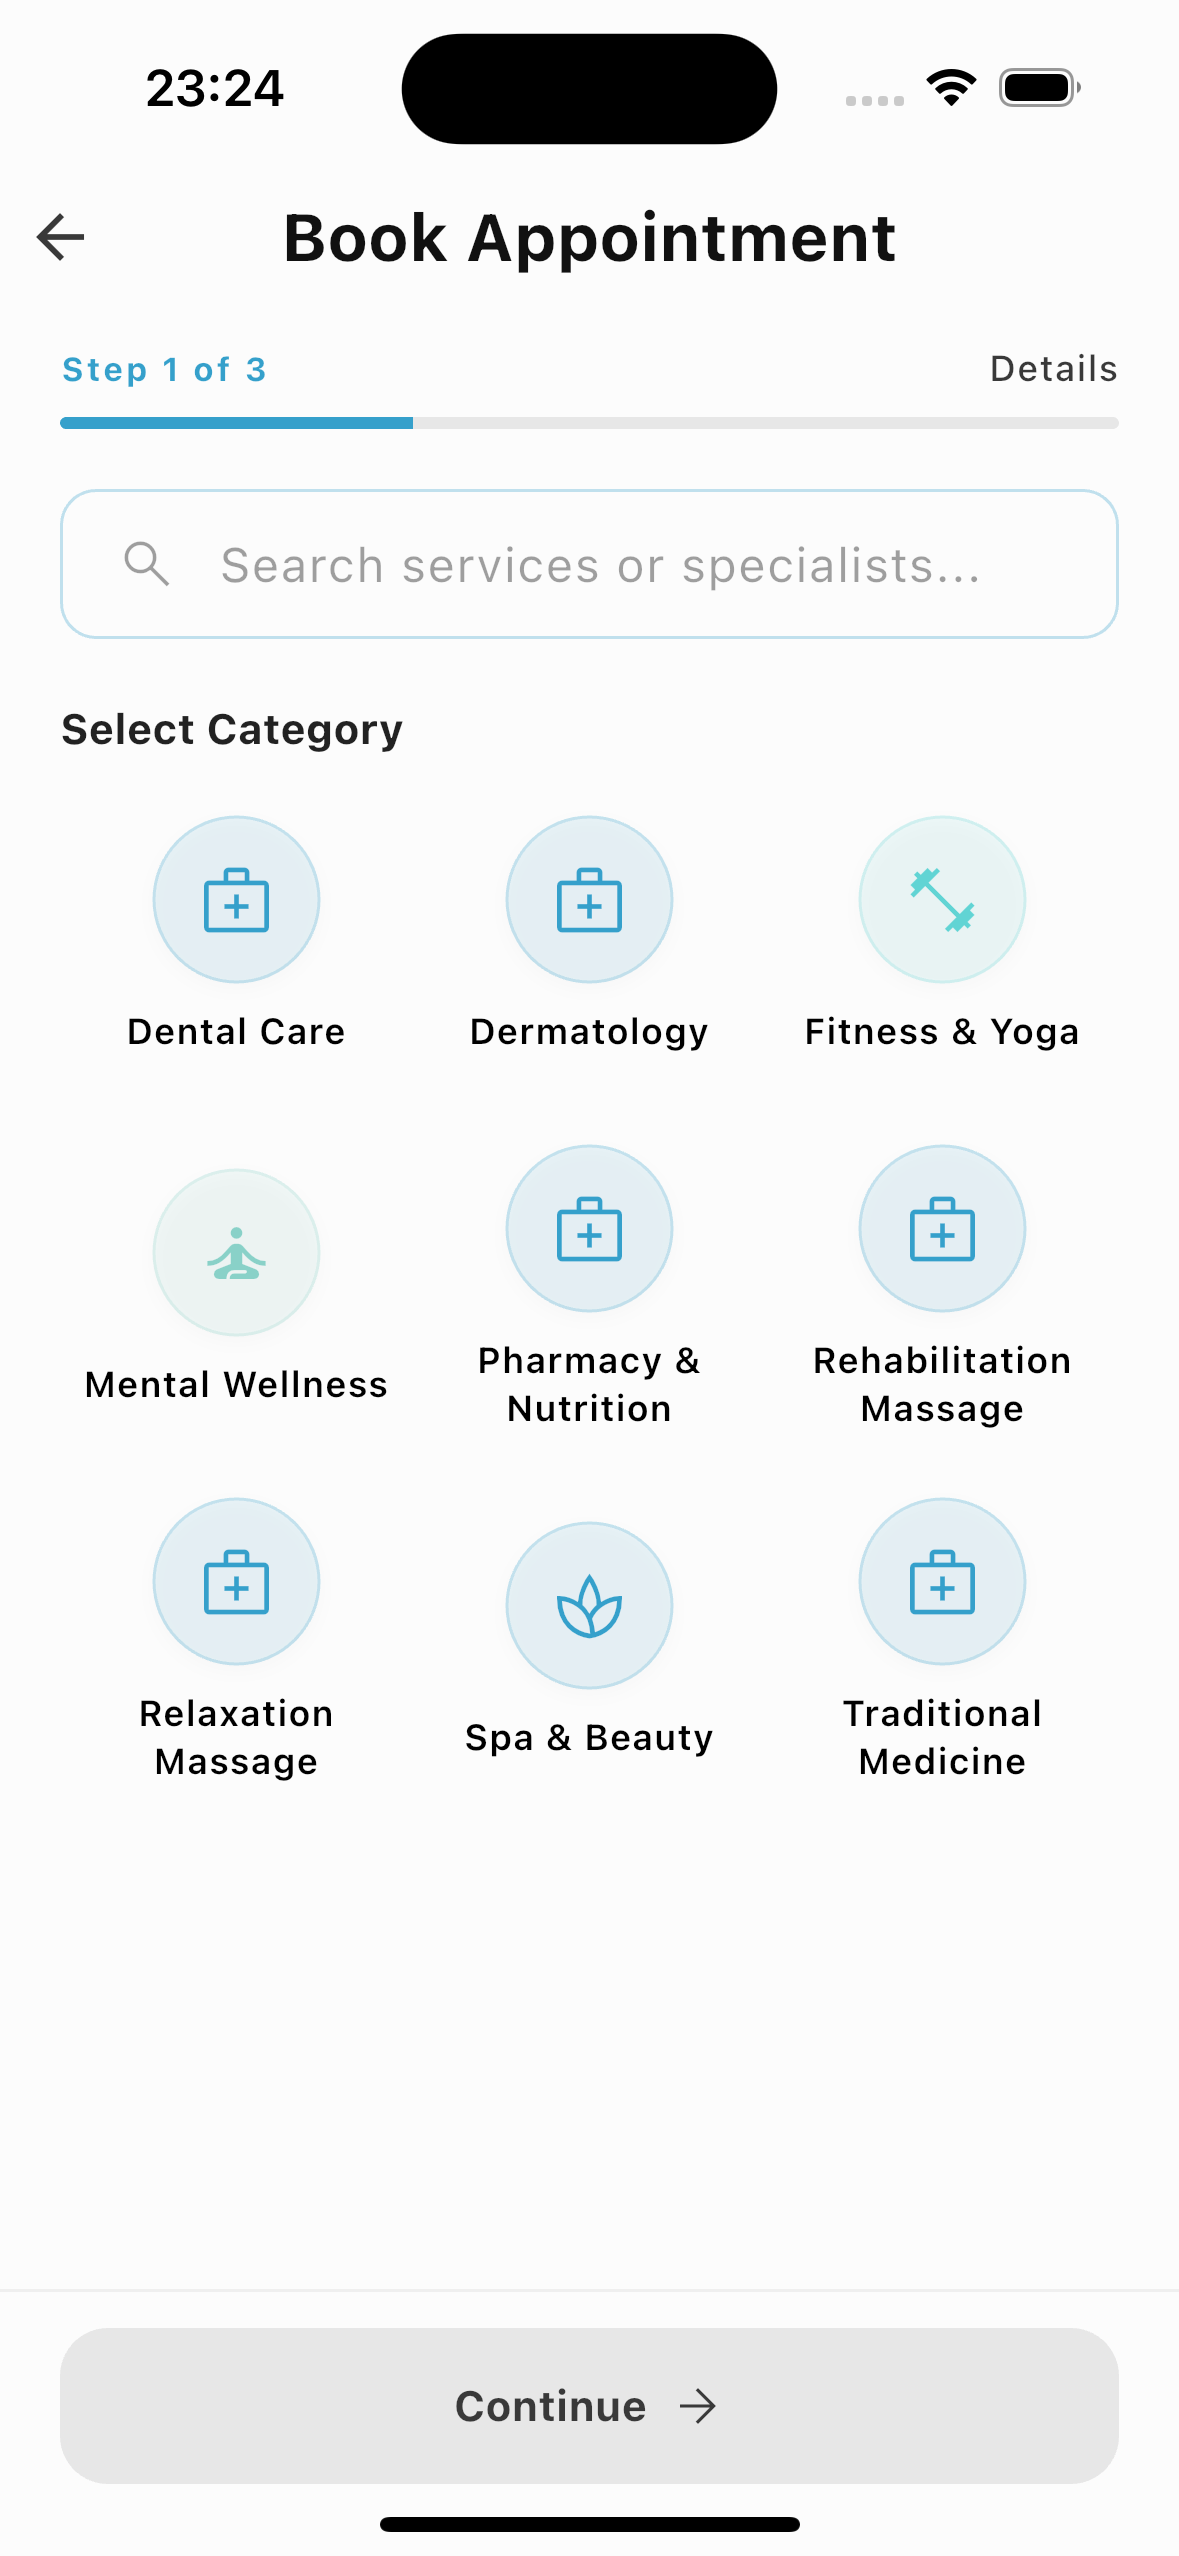
\includegraphics[width=\linewidth,height=0.28\textheight,keepaspectratio]{Images/Hiện thực/user_app/booking/fig_booking_step1_category.png}
    \caption{Chọn danh mục dịch vụ}
    \label{fig:booking_step1_category}
\end{subfigure}
\hfill
\begin{subfigure}[t]{0.48\linewidth}
    \centering
    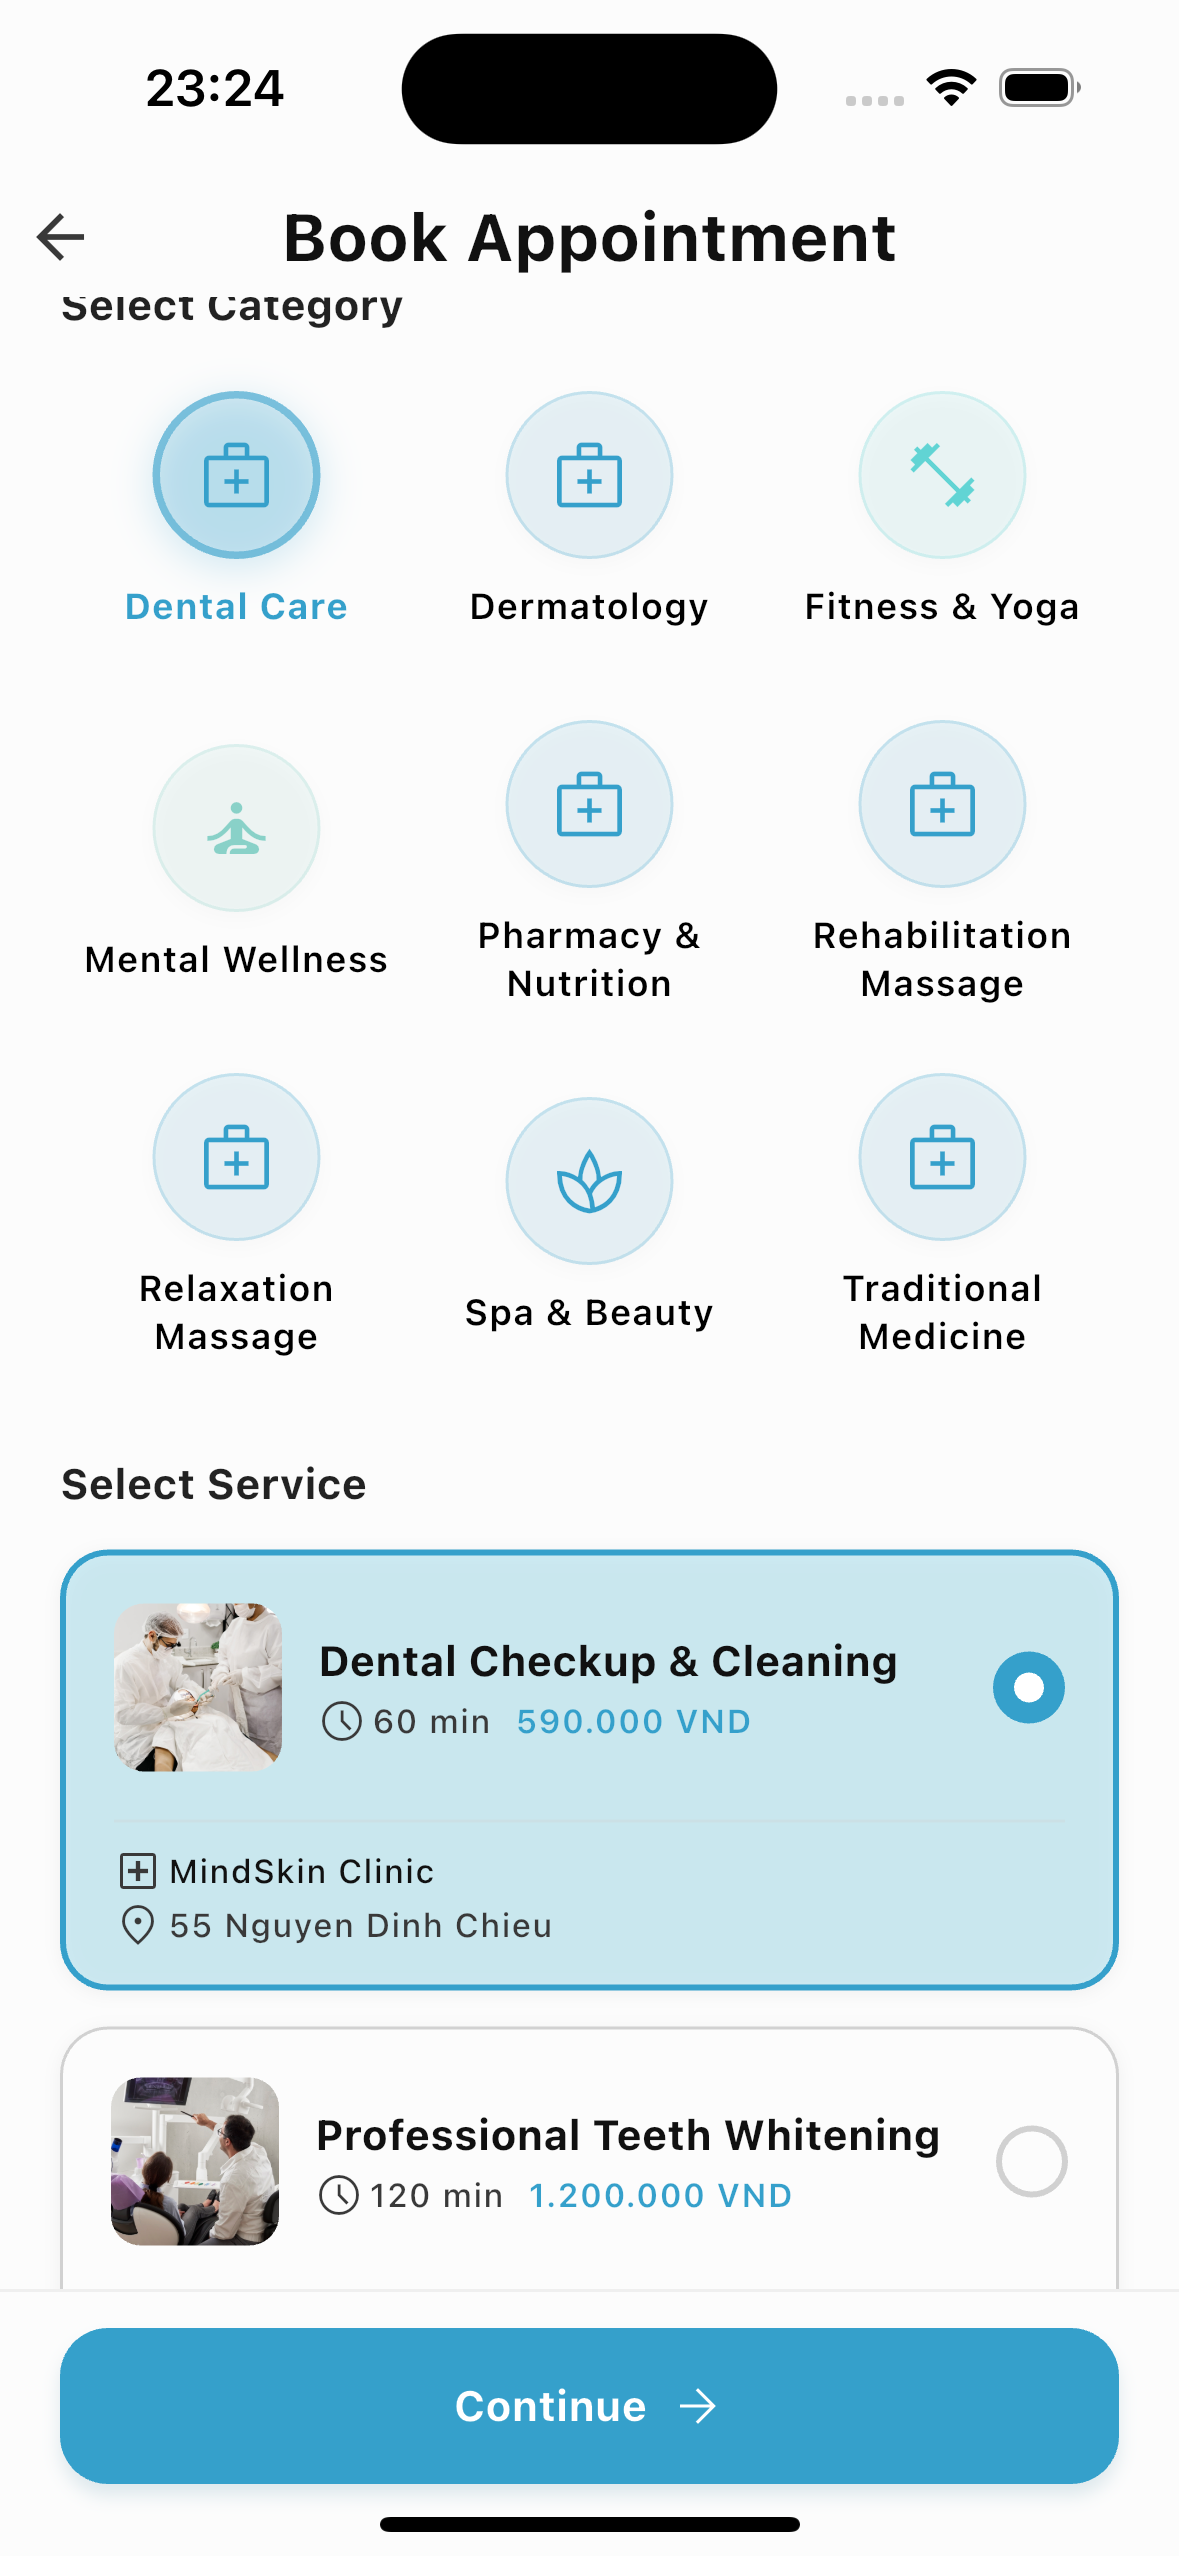
\includegraphics[width=\linewidth,height=0.28\textheight,keepaspectratio]{Images/Hiện thực/user_app/booking/fig_booking_step1_service.png}
    \caption{Chọn dịch vụ sau khi lọc danh mục}
    \label{fig:booking_step1_service}
\end{subfigure}
\par\medskip
\caption{Bước 1 -- Chọn danh mục và dịch vụ trong luồng Book Appointment}
\label{fig:booking_step1}
\end{figure}

\begin{figure}[H]
\centering
\captionsetup[subfigure]{font=small,justification=centering}
\captionsetup{skip=8pt}
\begin{subfigure}[t]{0.48\linewidth}
    \centering
    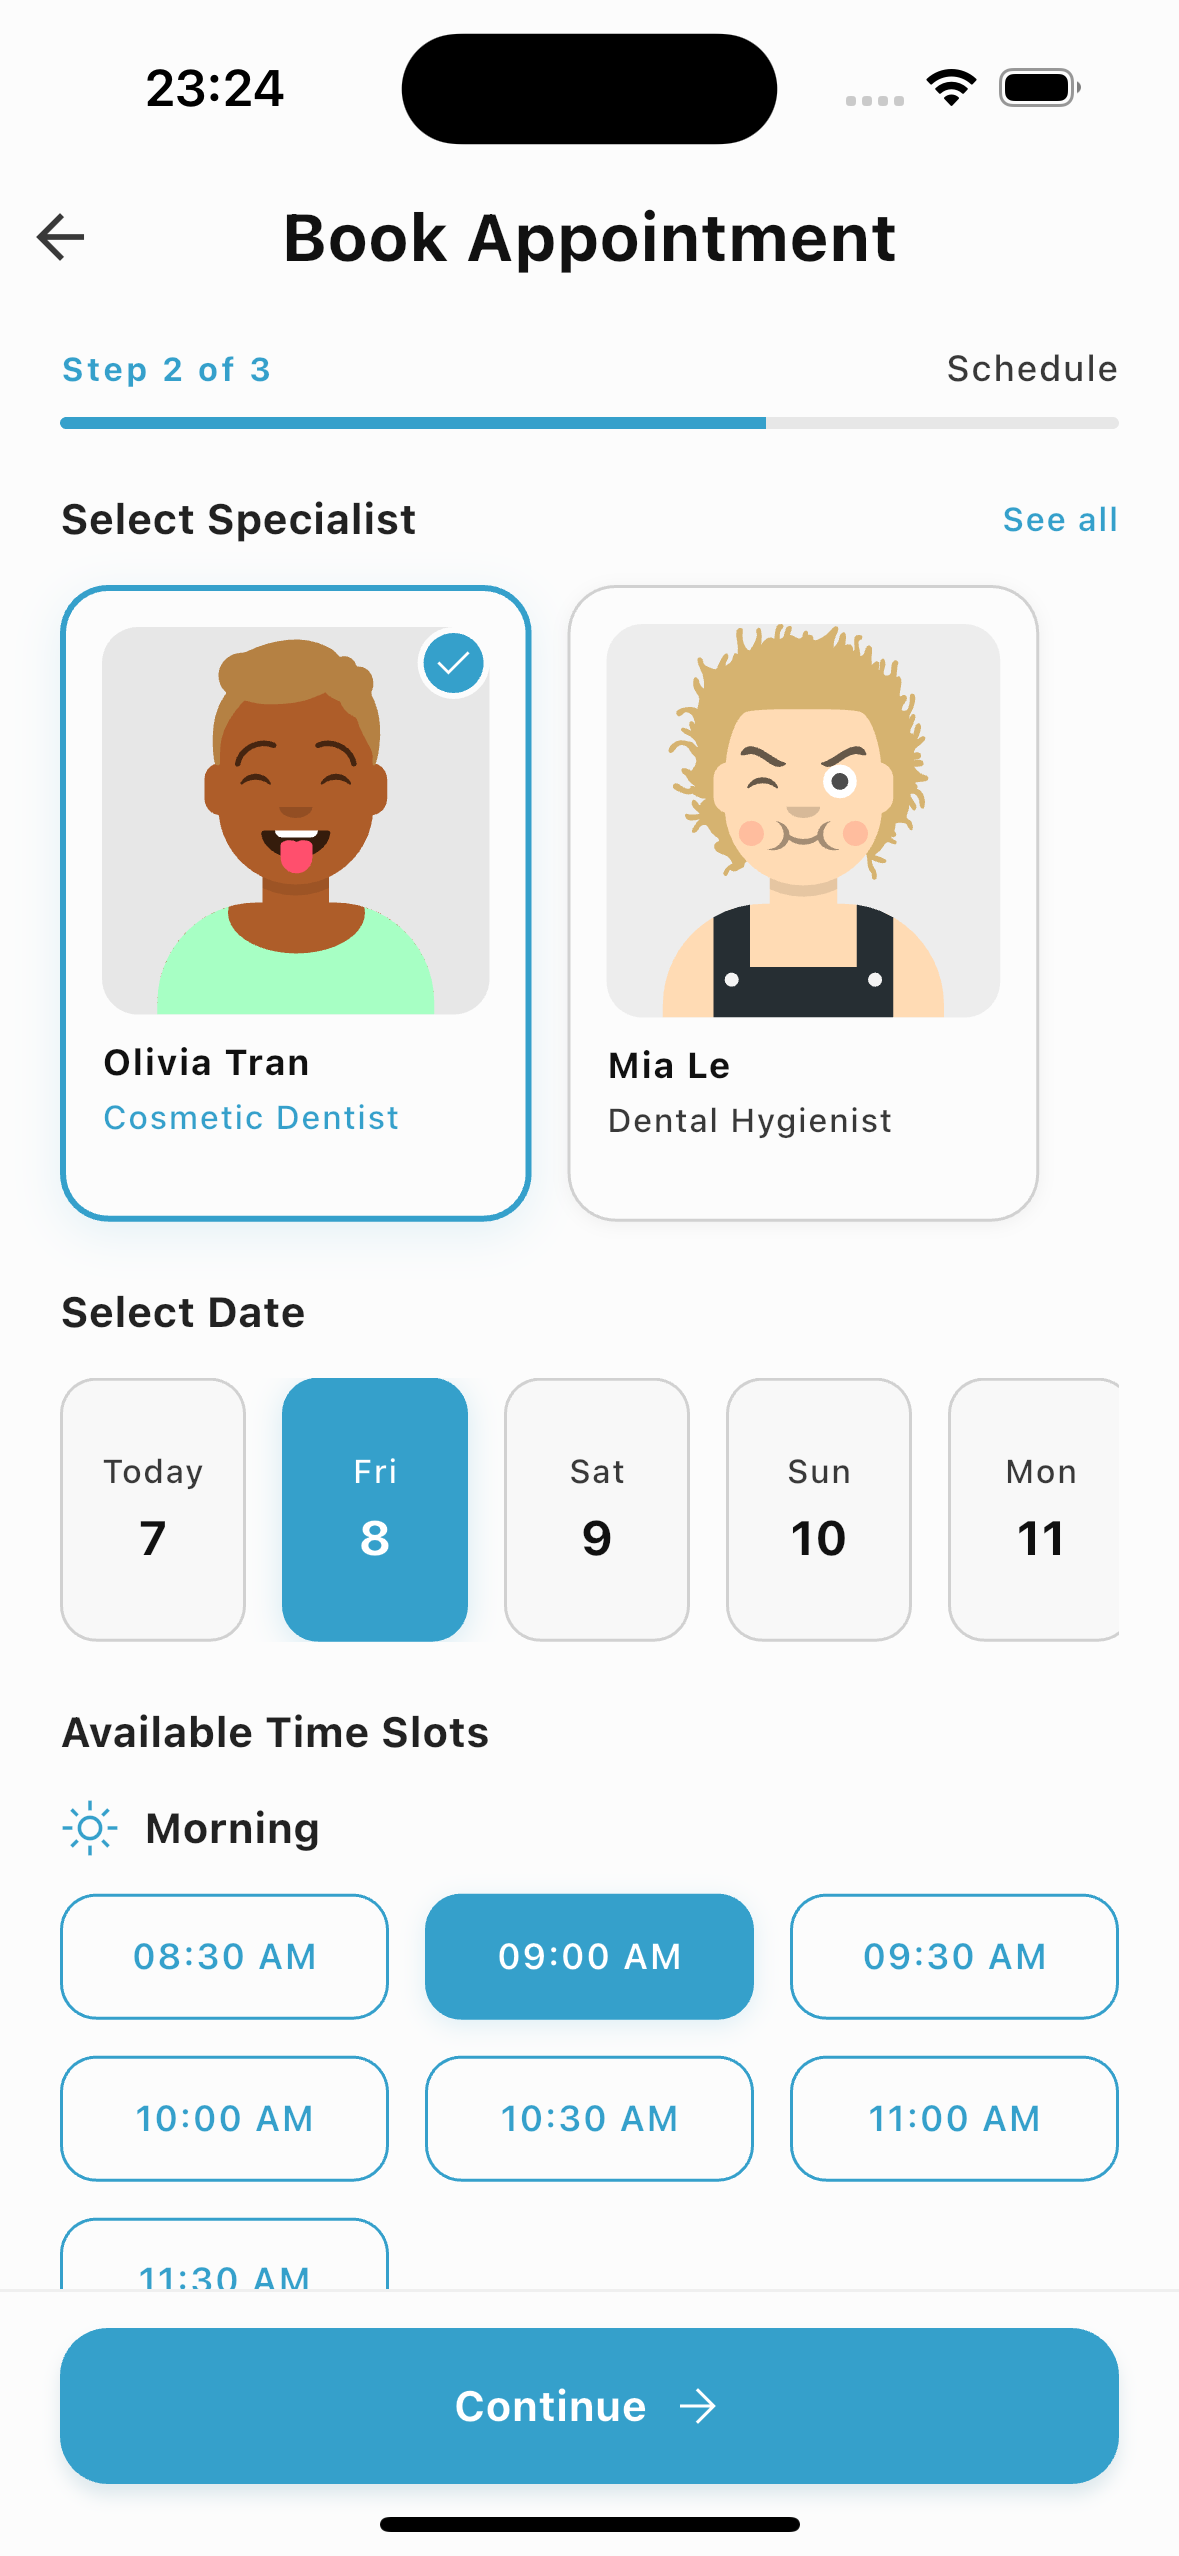
\includegraphics[width=\linewidth,height=0.28\textheight,keepaspectratio]{Images/Hiện thực/user_app/booking/fig_booking_step2_schedule.png}
    \caption{Chọn chuyên gia, ngày và khung giờ}
    \label{fig:booking_step2_schedule}
\end{subfigure}
\hfill
\begin{subfigure}[t]{0.48\linewidth}
    \centering
    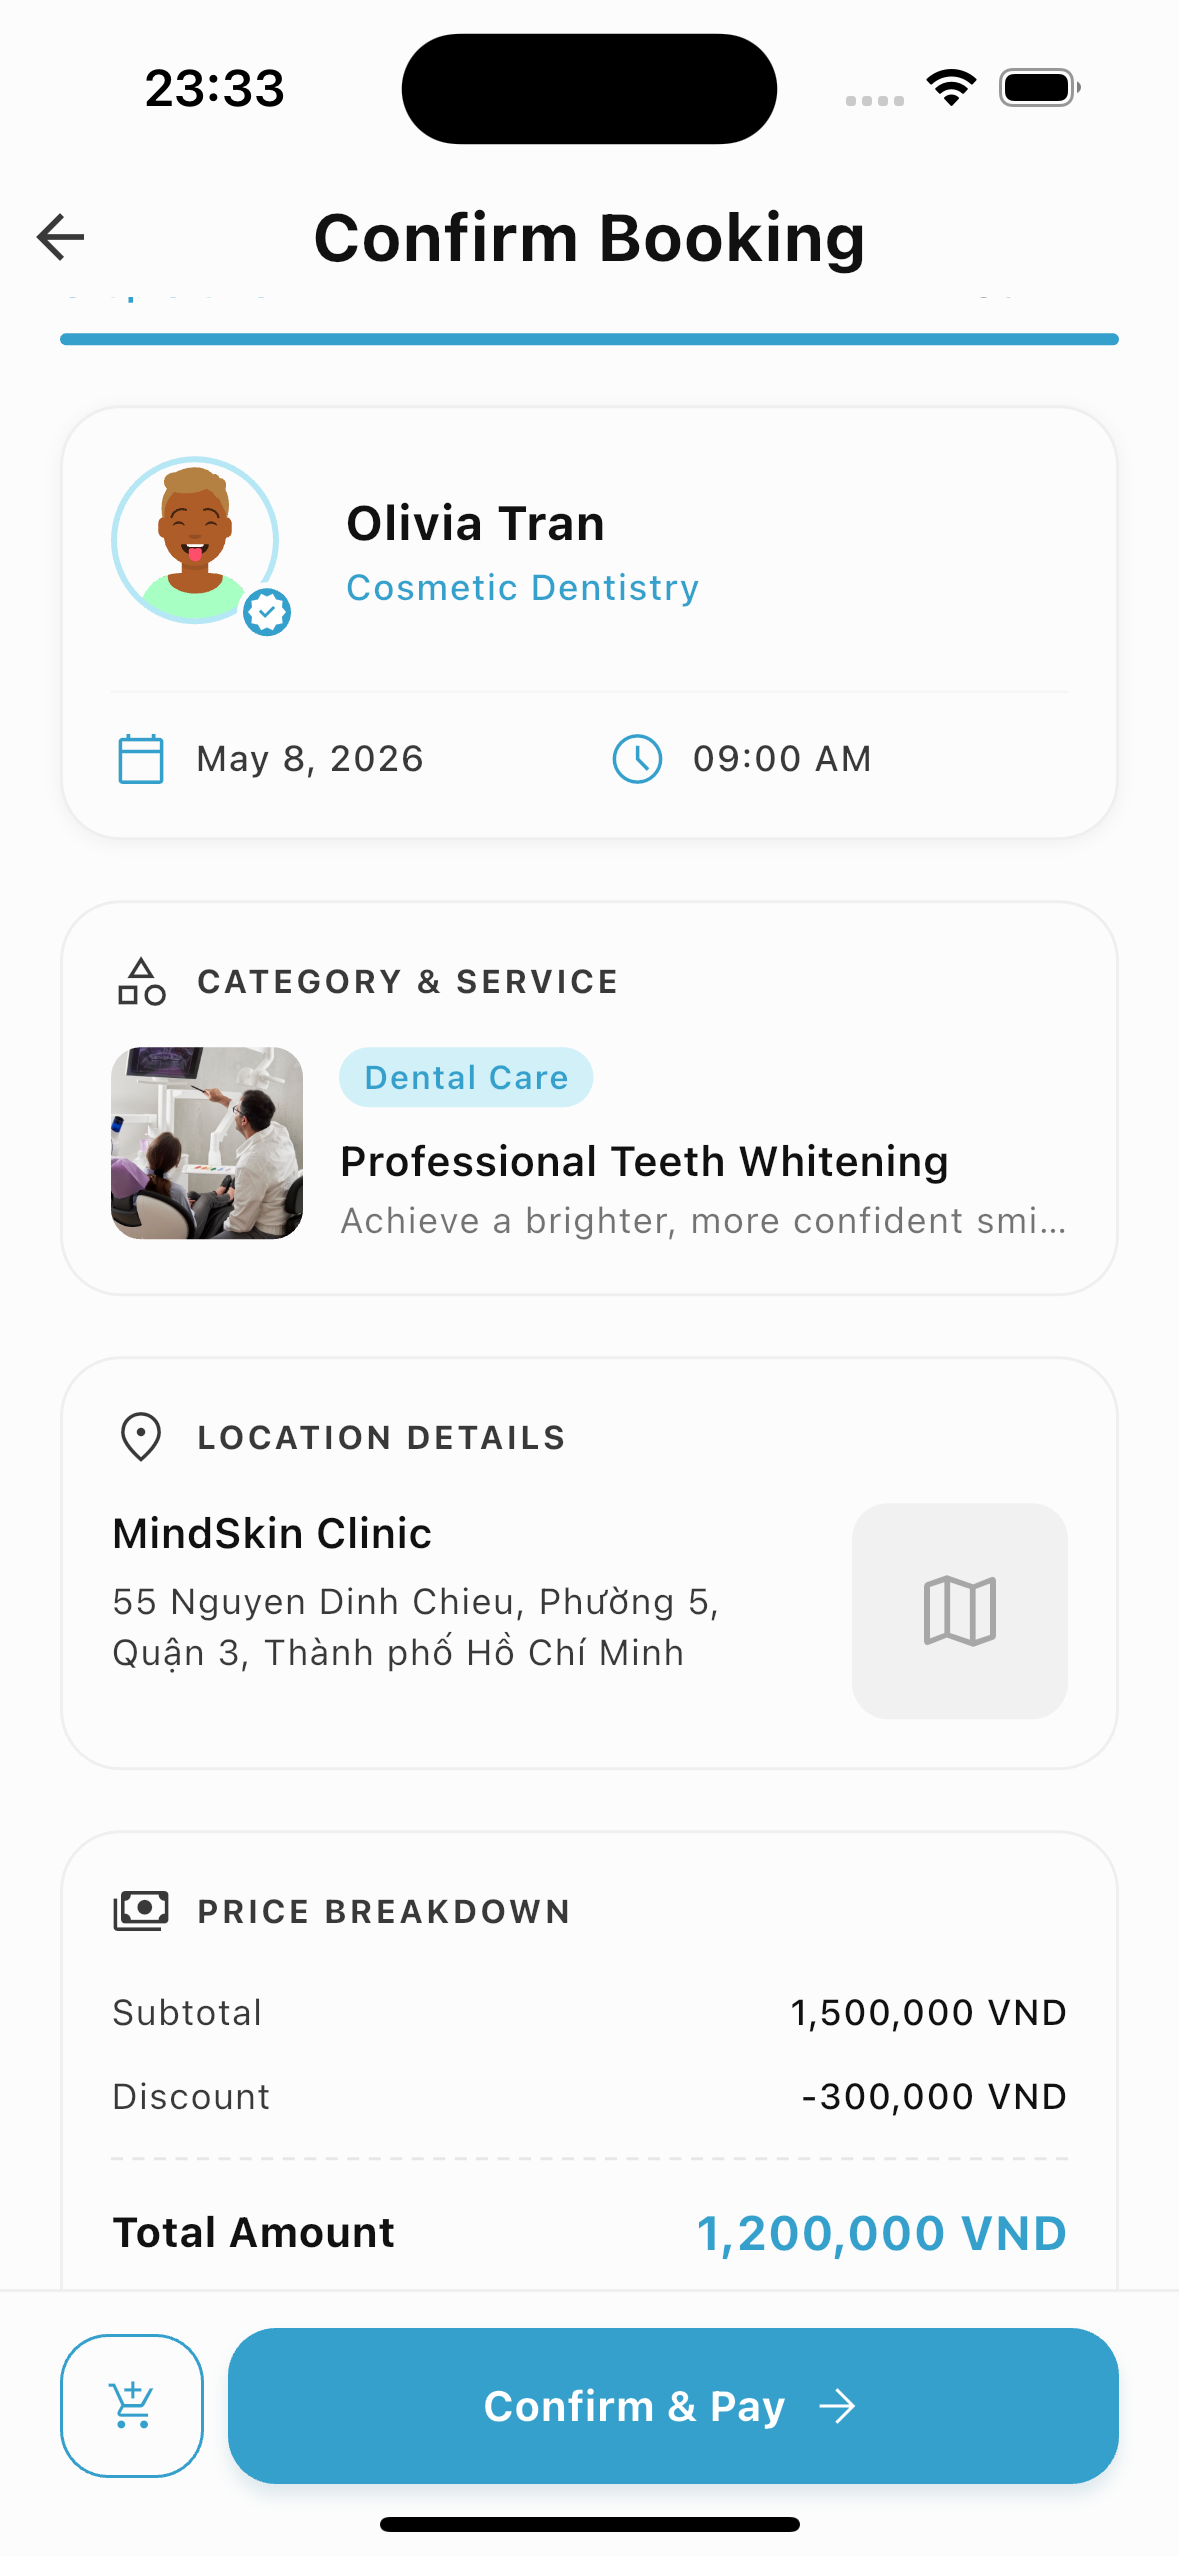
\includegraphics[width=\linewidth,height=0.28\textheight,keepaspectratio]{Images/Hiện thực/user_app/booking/fig_booking_step3_confirm.png}
    \caption{Xác nhận thông tin và bảng giá}
    \label{fig:booking_step3_confirm}
\end{subfigure}
\par\medskip
\caption{Bước 2 \& 3 -- Chọn lịch hẹn và xác nhận đặt lịch}
\label{fig:booking_step2_step3}
\end{figure}

\paragraph{Thanh toán (Checkout \& Payment)}

Sau khi xác nhận đặt lịch, người dùng được chuyển sang màn hình Checkout hiển thị tóm tắt đơn hàng (phòng khám, dịch vụ, chuyên gia, giá) kèm tùy chọn quy đổi xu (Redeem Coins). Hệ thống hỗ trợ ba phương thức thanh toán:

\begin{itemize}
    \item \textbf{Credit/Debit Card:} Thanh toán quốc tế qua cổng Stripe.
    \item \textbf{E-Wallet (MoMo/ZaloPay):} Thanh toán nội địa qua ví điện tử MoMo. Khi chọn phương thức này, ứng dụng mở WebView đến cổng \texttt{test-payment.momo.vn}, hiển thị mã đơn hàng và số tiền để người dùng xác nhận bằng ví MoMo.
    \item \textbf{Pay Later:} Cho phép đặt lịch trước, thanh toán sau tại phòng khám.
\end{itemize}

\begin{figure}[H]
\centering
\captionsetup[subfigure]{font=small,justification=centering}
\captionsetup{skip=8pt}
\begin{subfigure}[t]{0.48\linewidth}
    \centering
    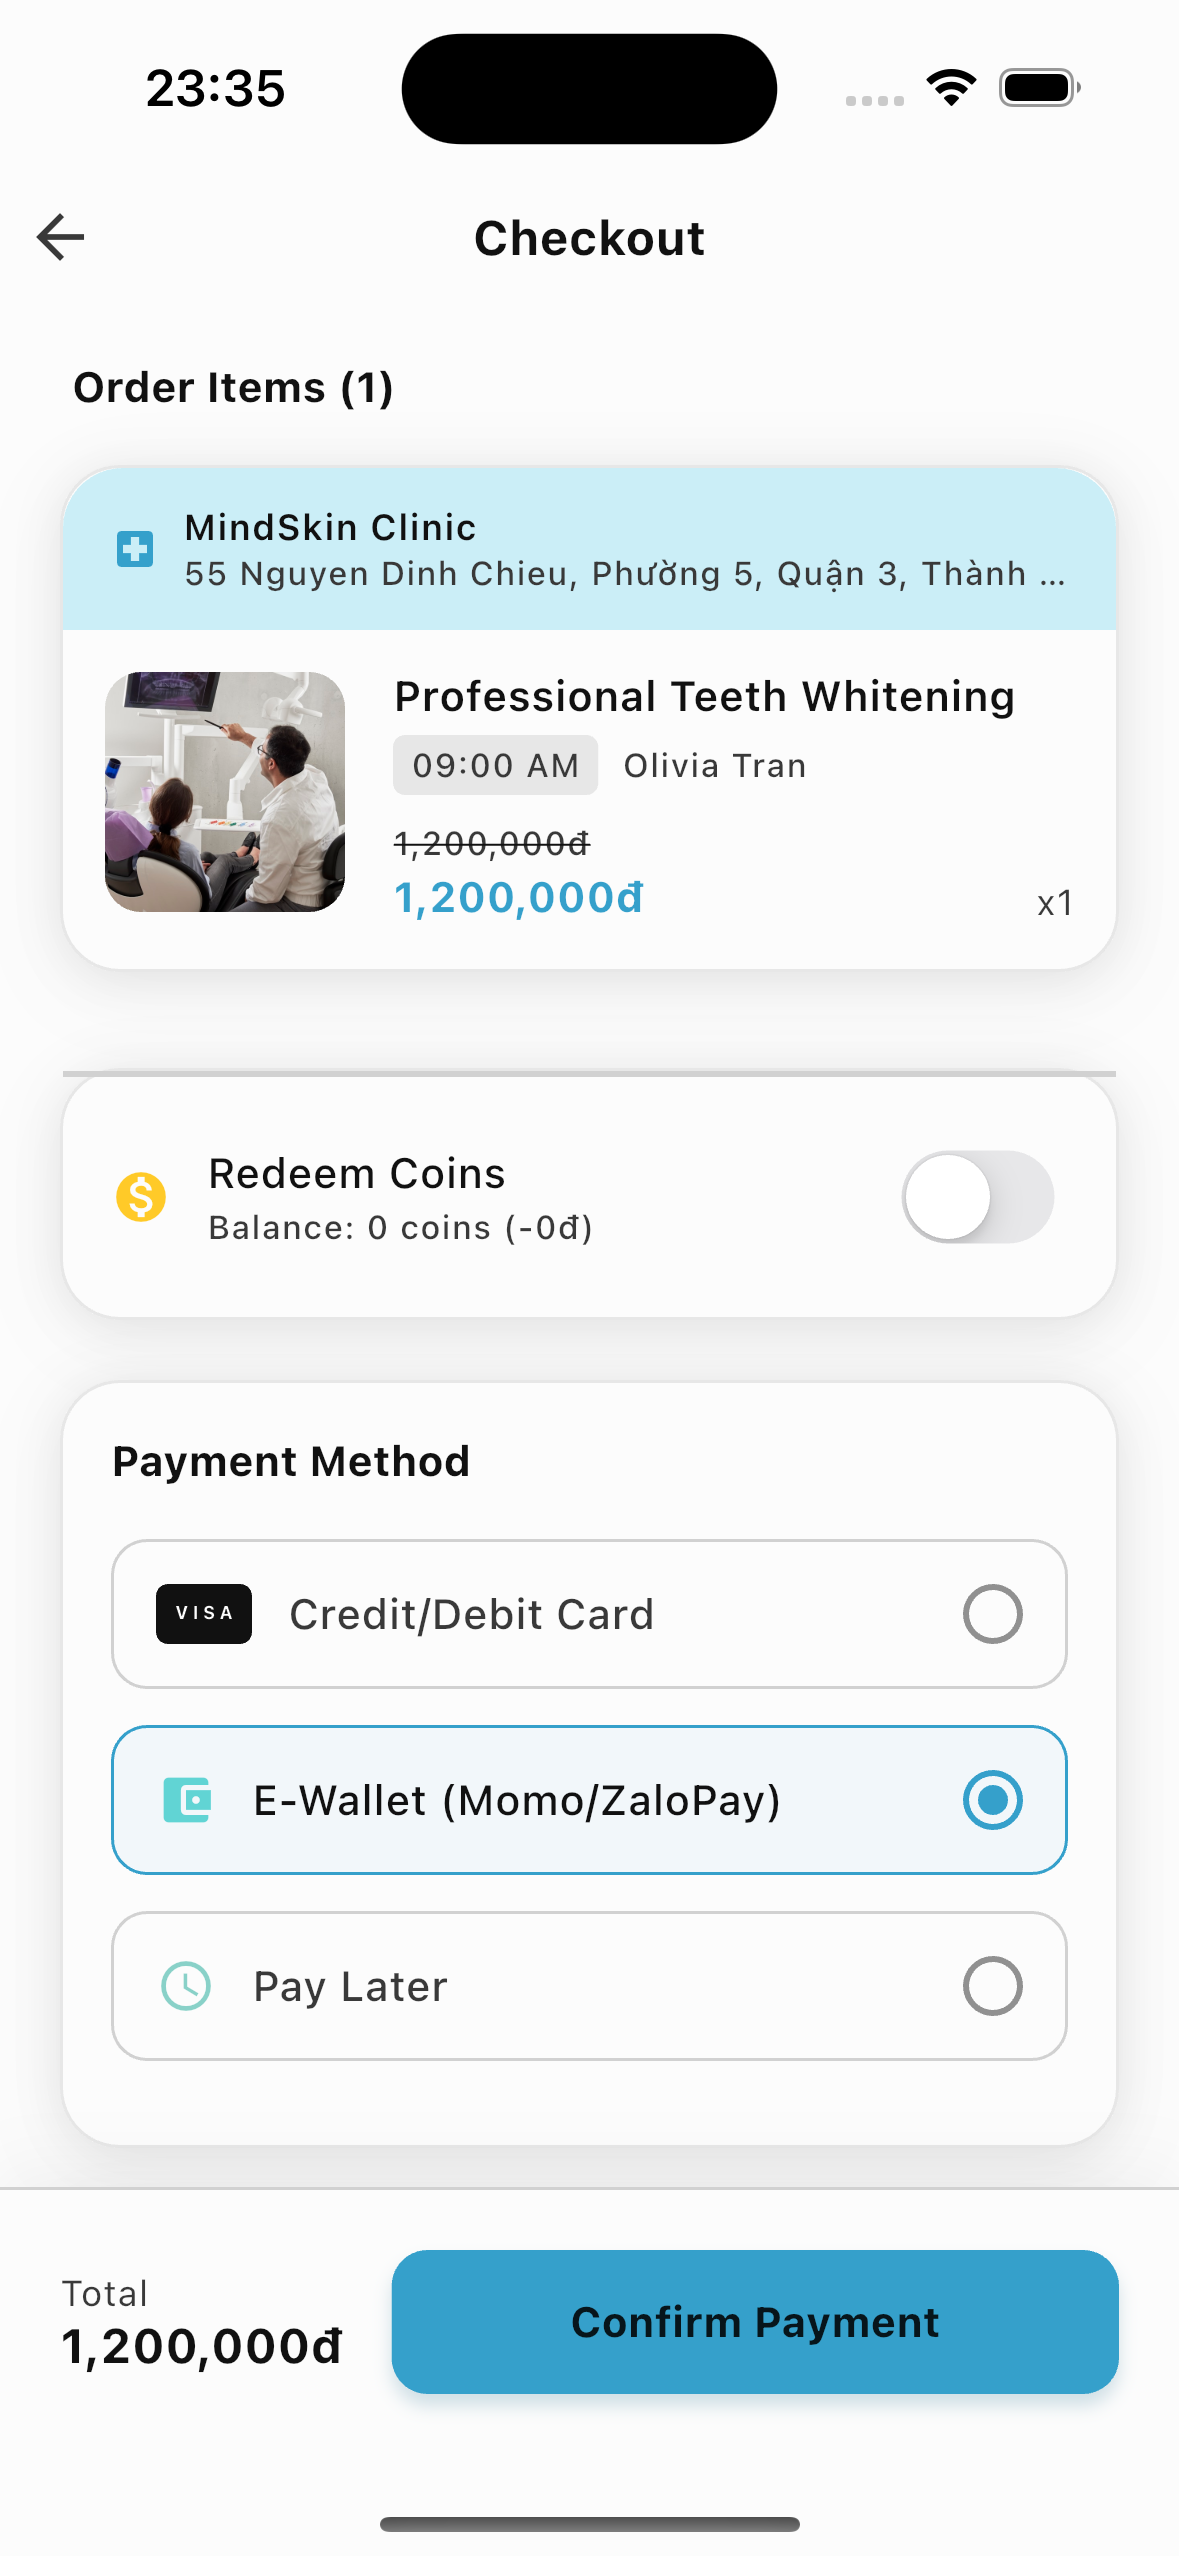
\includegraphics[width=\linewidth,height=0.28\textheight,keepaspectratio]{Images/Hiện thực/user_app/booking/fig_booking_checkout.png}
    \caption{Chọn phương thức thanh toán}
    \label{fig:booking_checkout}
\end{subfigure}
\hfill
\begin{subfigure}[t]{0.48\linewidth}
    \centering
    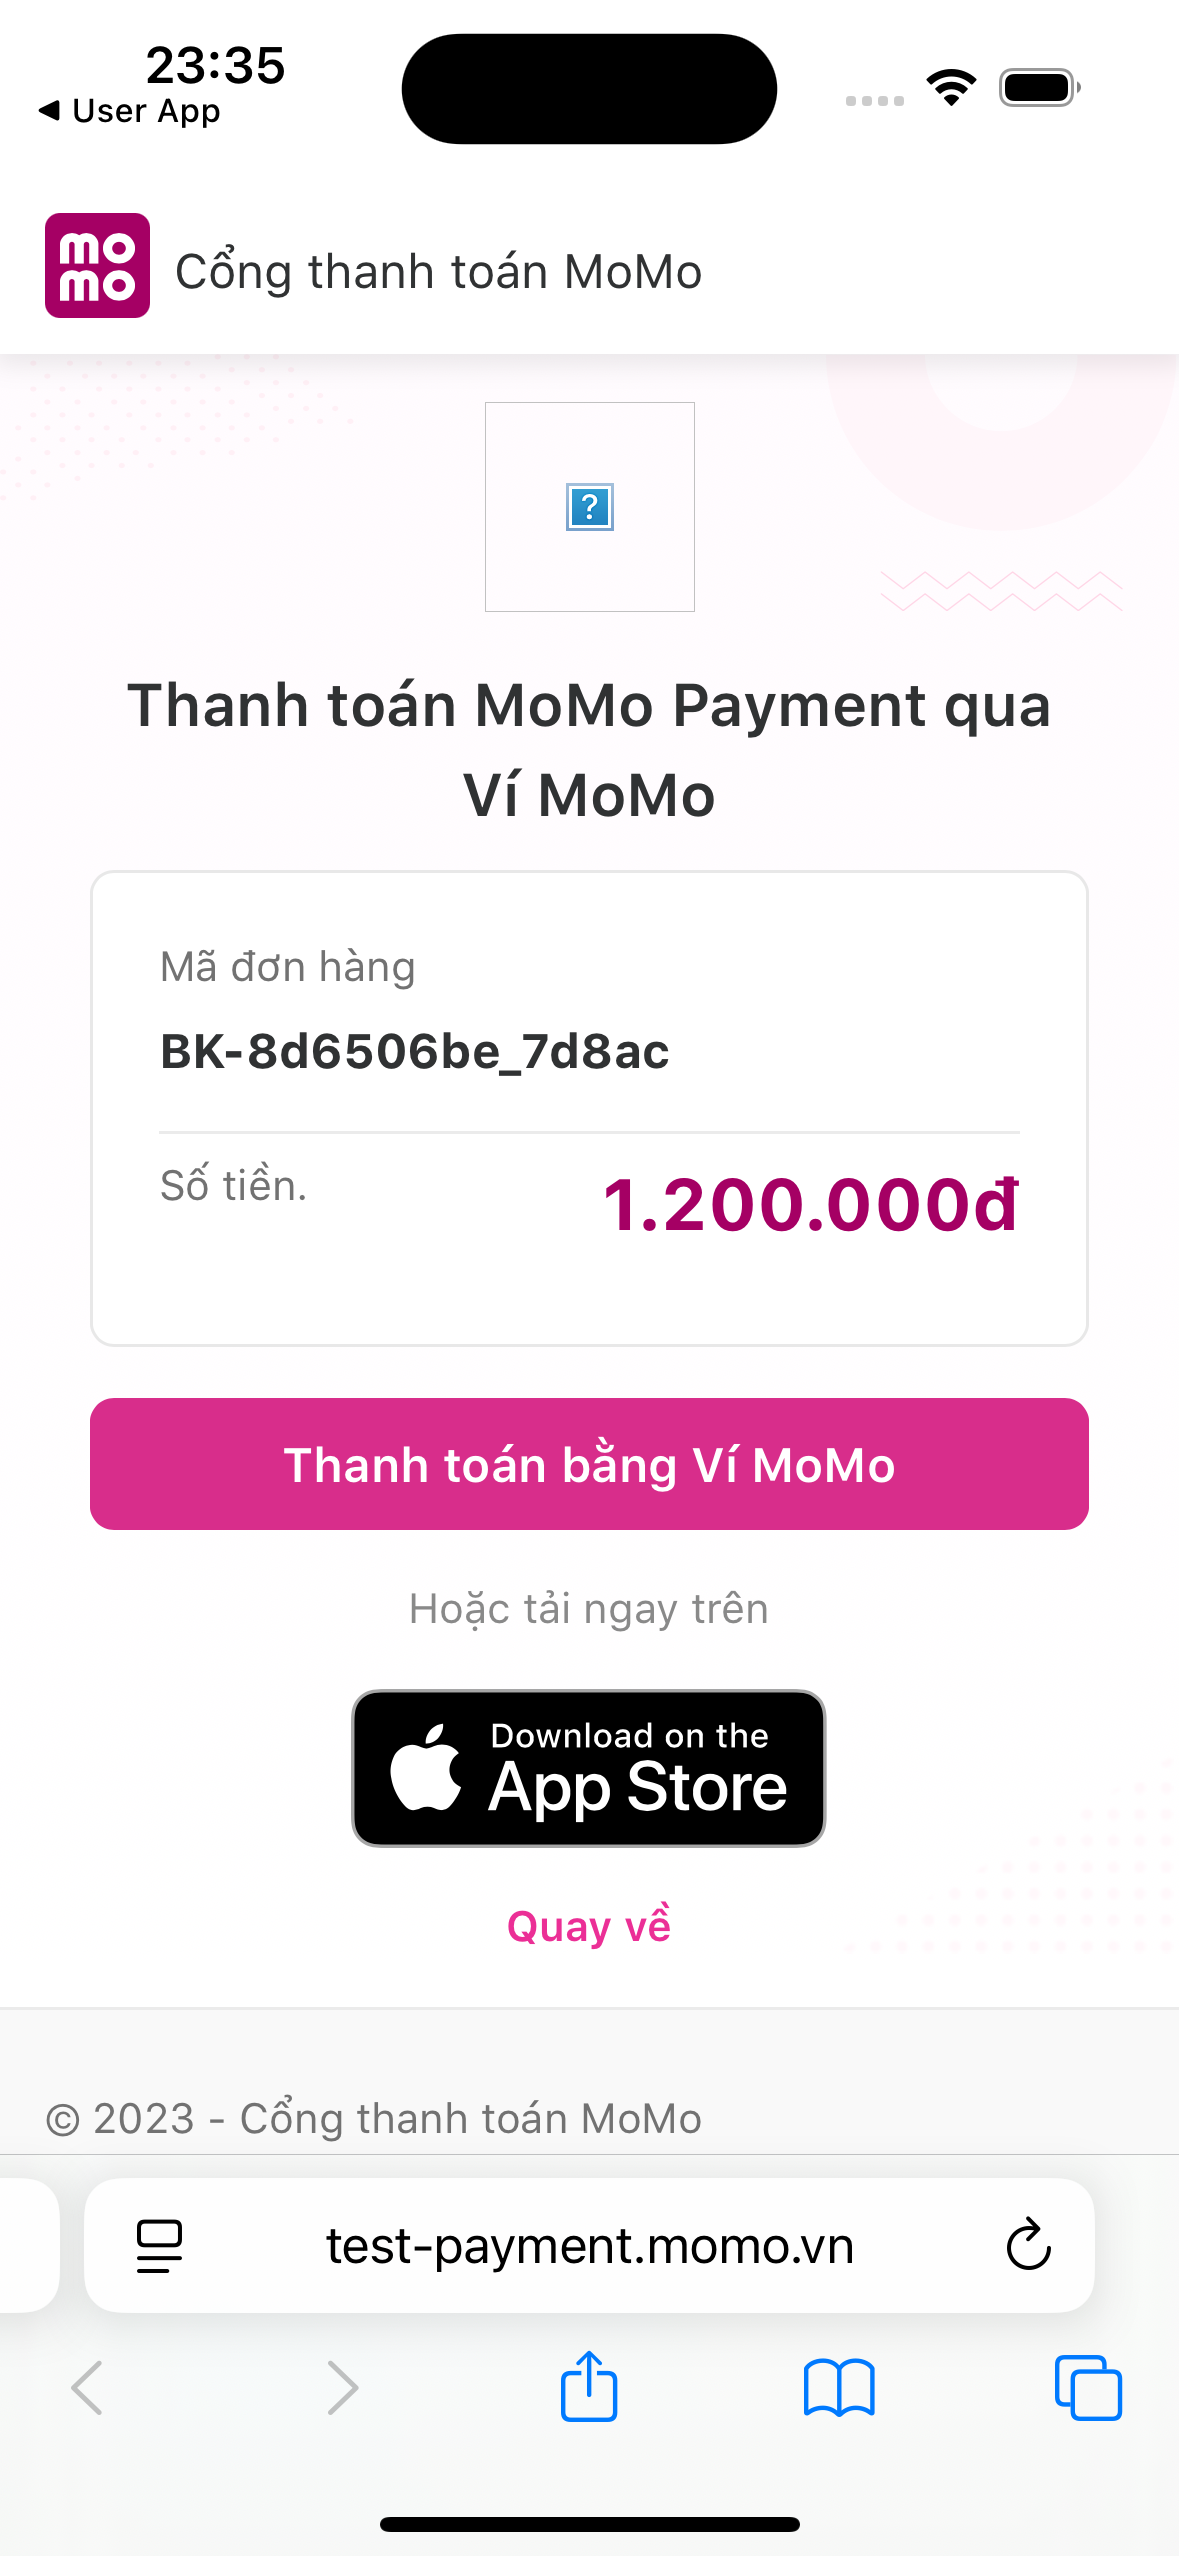
\includegraphics[width=\linewidth,height=0.28\textheight,keepaspectratio]{Images/Hiện thực/user_app/booking/fig_booking_momo_payment.png}
    \caption{Cổng thanh toán MoMo}
    \label{fig:booking_momo_payment}
\end{subfigure}
\par\medskip
\caption{Luồng Checkout và thanh toán qua ví điện tử MoMo}
\label{fig:booking_checkout_flow}
\end{figure}

\textbf{Tính năng kỹ thuật:}

\begin{itemize}
    \item \textbf{Payment Gateway Integration:} Stripe (quốc tế) và MoMo (nội địa), với luồng IPN/Webhook server-to-server xác nhận giao dịch.
    \item \textbf{Redeem Coins:} Người dùng có thể quy đổi xu tích lũy để giảm giá trực tiếp trên tổng đơn hàng.
    \item \textbf{Idempotency:} Sử dụng mã đơn hàng duy nhất (\texttt{BK-*}) ngăn double charge khi retry.
    \item \textbf{Distributed Lock:} Redis Redlock khóa slot trong 10 phút (TTL) từ lúc tạo draft order đến khi thanh toán hoàn tất.
\end{itemize}

\paragraph{Trò chuyện với trợ lý AI (Chat with Dr. AI)}

\begin{figure}[H]
\centering
\begin{subfigure}[b]{0.48\linewidth}
    \centering
    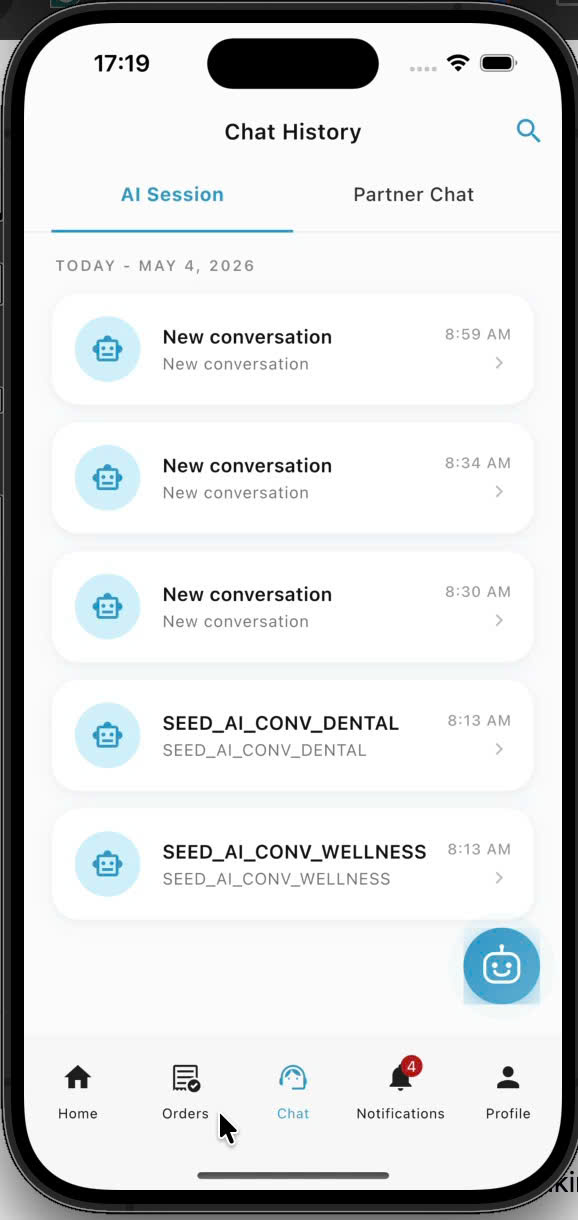
\includegraphics[width=\linewidth,height=0.42\textheight,keepaspectratio,trim=30 40 30 40,clip]{Images/Hiện thực/user/fig_user_chat_history.jpg}
    \caption{Lịch sử chat AI Session (zoom)}
\end{subfigure}
\hfill
\begin{subfigure}[b]{0.48\linewidth}
    \centering
    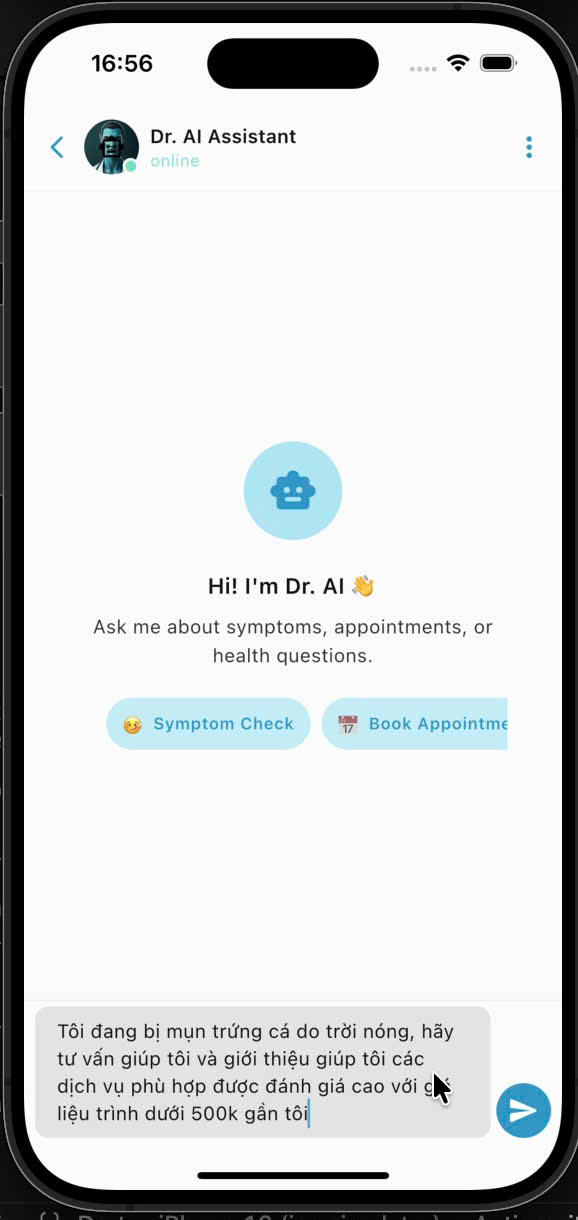
\includegraphics[width=\linewidth,height=0.42\textheight,keepaspectratio,trim=30 40 30 40,clip]{Images/Hiện thực/user/fig_user_chat_ask_2.jpg}
    \caption{Cuộc trò chuyện chi tiết (zoom)}
\end{subfigure}
\par\medskip
\caption{Màn hình Chat History - Tư vấn AI}
\label{fig:user_chat_history}
\end{figure}

\begin{itemize}
    \item \textbf{Thao tác mở hội thoại:} Người dùng chọn một phiên chat trong \textit{AI Session} để xem lịch sử chi tiết.
    \item \textbf{Thao tác gửi câu hỏi:} Nhập nội dung ở ô tin nhắn và nhấn nút gửi để nhận phản hồi từ Dr. AI.
\end{itemize}

\textbf{Tính năng kỹ thuật:}

\begin{itemize}
    \item \textbf{LLM Integration:} Chat AI dùng GPT-4 hoặc Llama.
    \item \textbf{Streaming Response:} Stream từng token qua SSE/WebSocket.
    \item \textbf{Context Preservation:} Lưu context trên server.
    \item \textbf{Service Recommendation:} Gợi ý dịch vụ phù hợp.
\end{itemize}

\paragraph{Chi tiết dịch vụ (Service Detail)}

\begin{figure}[H]
\centering
\captionsetup[subfigure]{font=small,justification=centering}
\captionsetup{skip=6pt}
\begin{subfigure}[t]{0.48\linewidth}
    \centering
    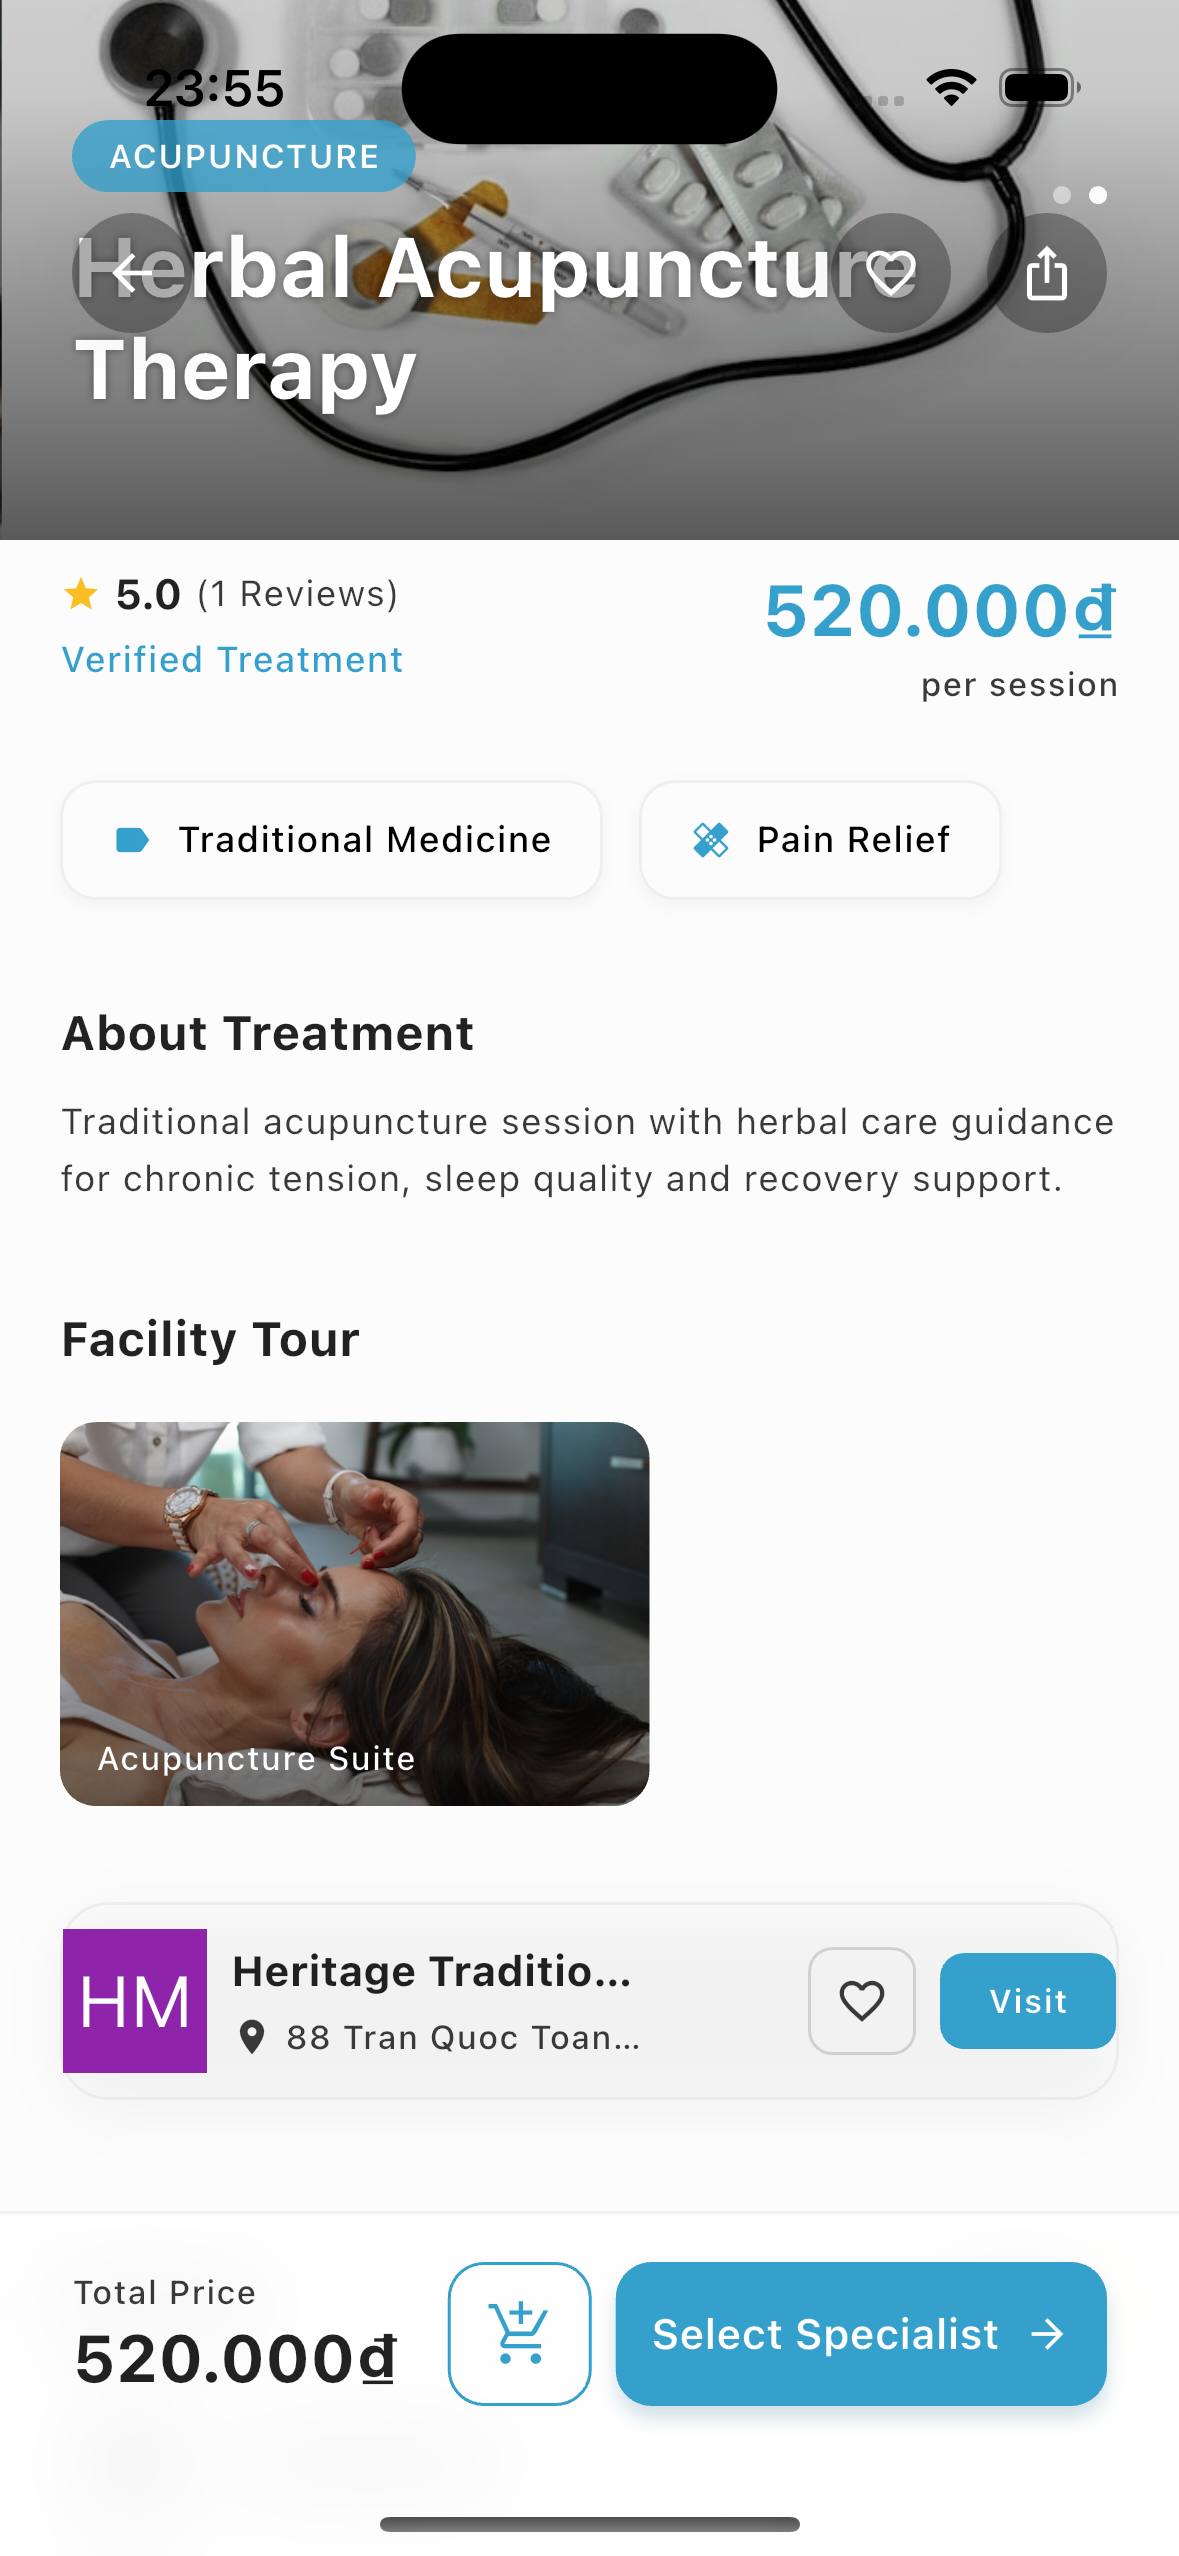
\includegraphics[width=\linewidth,height=0.4\textheight,keepaspectratio]{Images/Hiện thực/user_app/service_details/Simulator Screenshot - iPhone 16 - 2026-05-07 at 23.55.30.png}
    \caption{Tổng quan dịch vụ}
    \label{fig:service_detail_overview}
\end{subfigure}
\hfill
\begin{subfigure}[t]{0.48\linewidth}
    \centering
    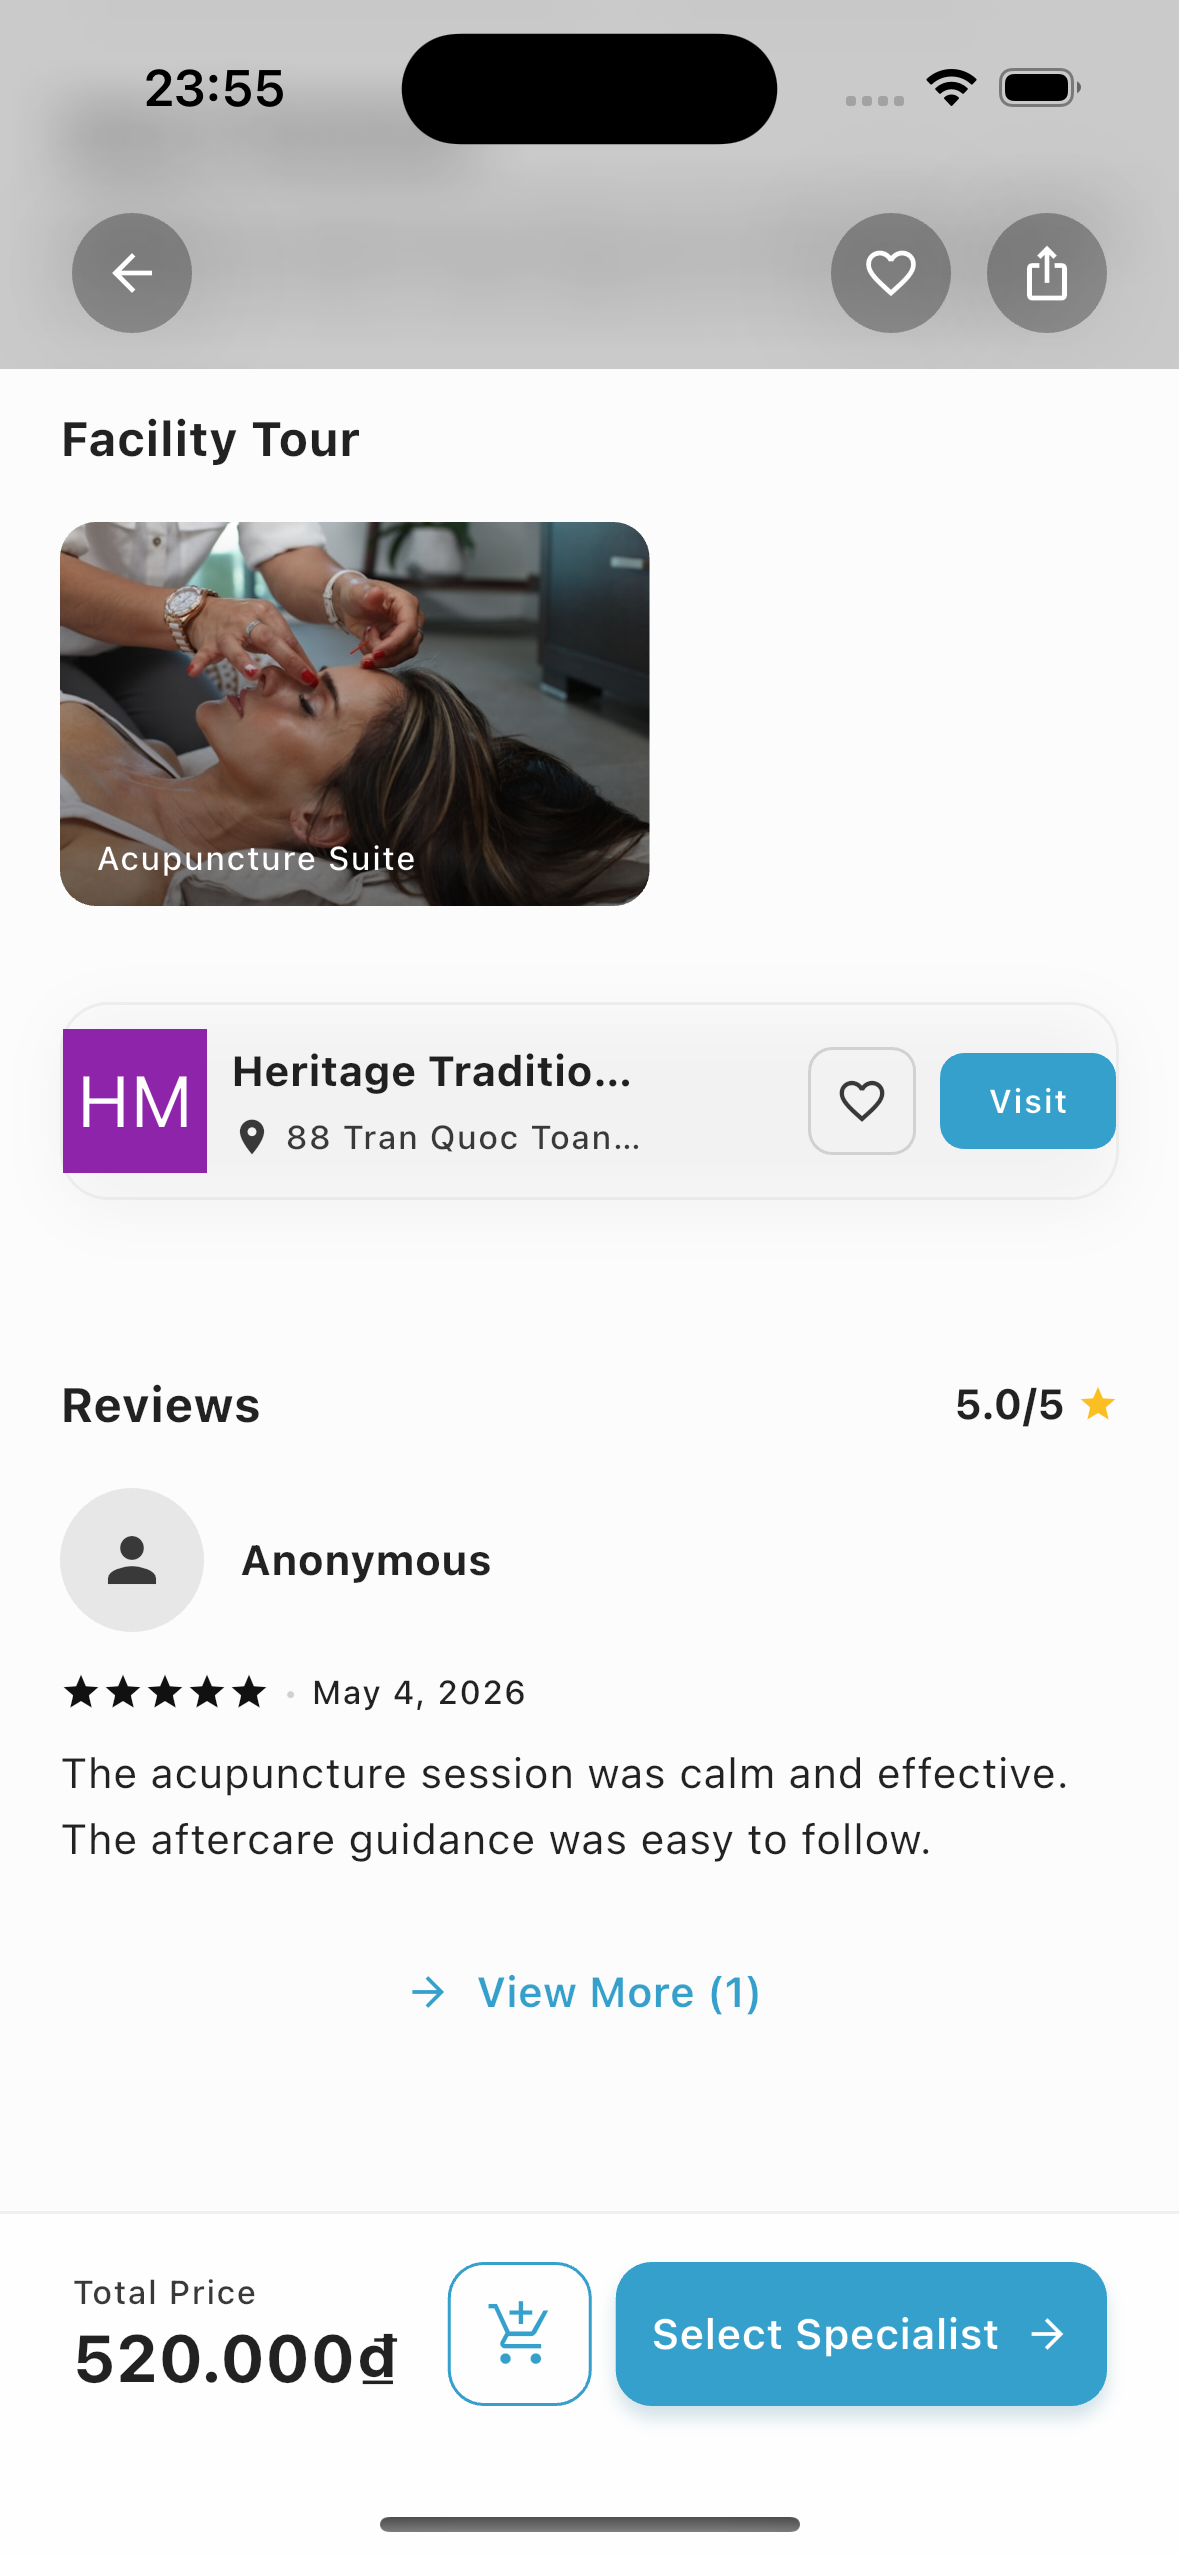
\includegraphics[width=\linewidth,height=0.4\textheight,keepaspectratio]{Images/Hiện thực/user_app/service_details/Simulator Screenshot - iPhone 16 - 2026-05-07 at 23.55.38.png}
    \caption{Phần đánh giá và nhận xét}
    \label{fig:service_detail_reviews}
\end{subfigure}
\par\medskip
\caption{Luồng Service Detail trên ứng dụng người dùng}
\label{fig:user_service_detail_flow}
\end{figure}

\begin{figure}[H]
\centering
\captionsetup[subfigure]{font=small,justification=centering}
\captionsetup{skip=8pt}
\begin{subfigure}[t]{0.48\linewidth}
    \centering
    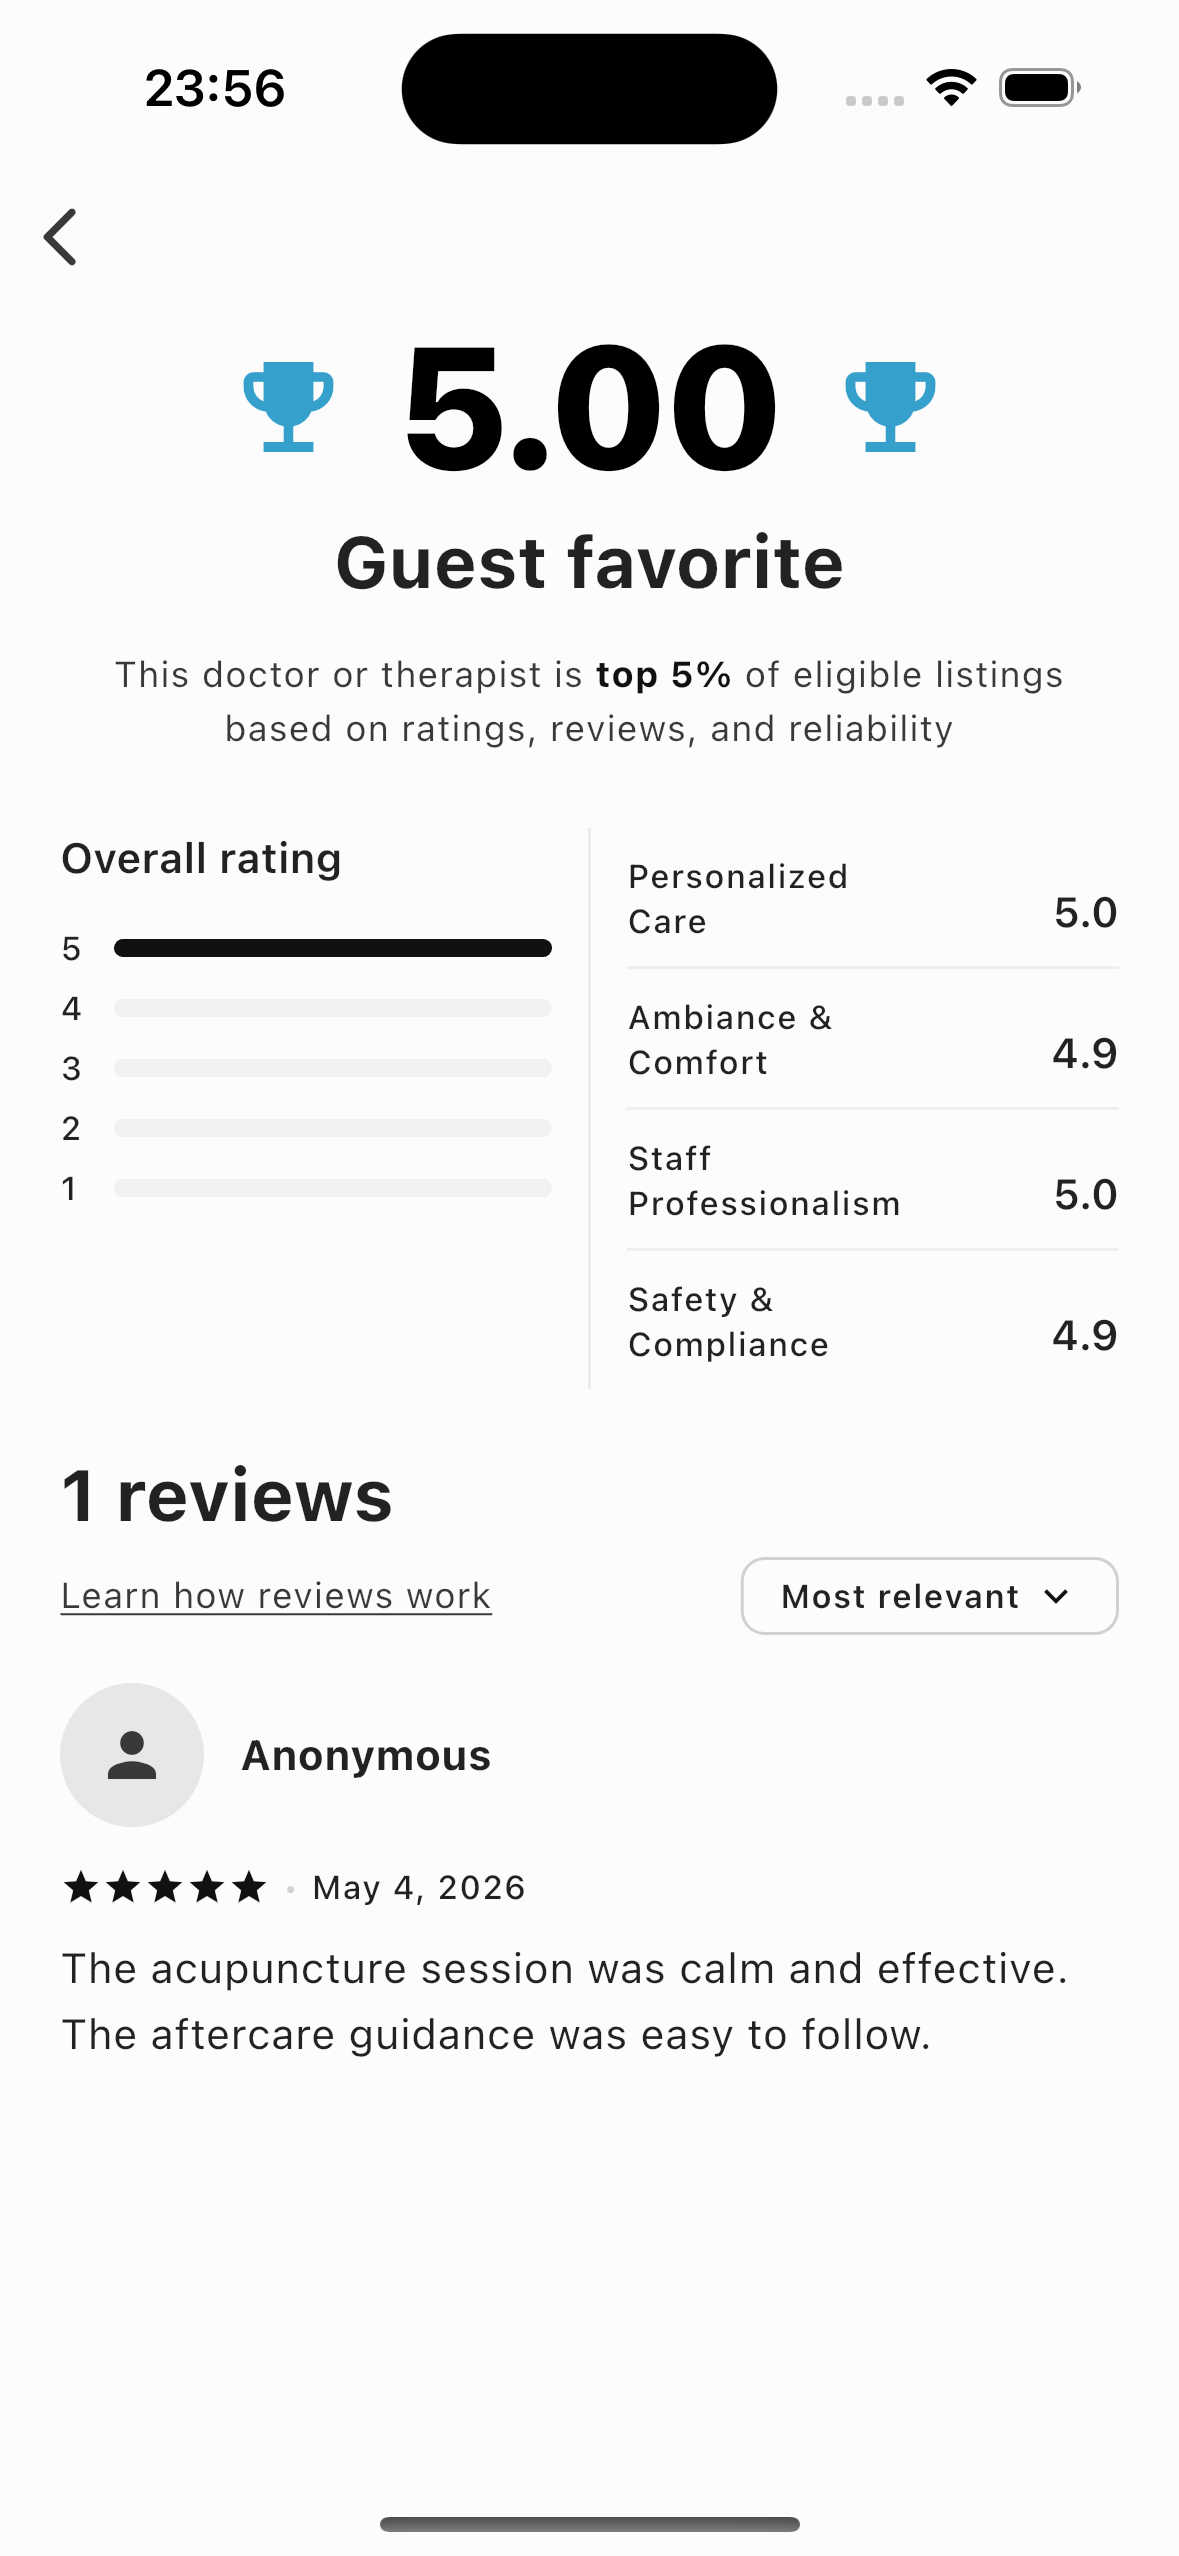
\includegraphics[width=\linewidth,height=0.4\textheight,keepaspectratio]{Images/Hiện thực/user_app/service_details/Simulator Screenshot - iPhone 16 - 2026-05-07 at 23.56.00.png}
    \caption{Bảng xếp hạng chi tiết}
    \label{fig:service_detail_ratings}
\end{subfigure}
\hfill
\begin{subfigure}[t]{0.48\linewidth}
    \centering
    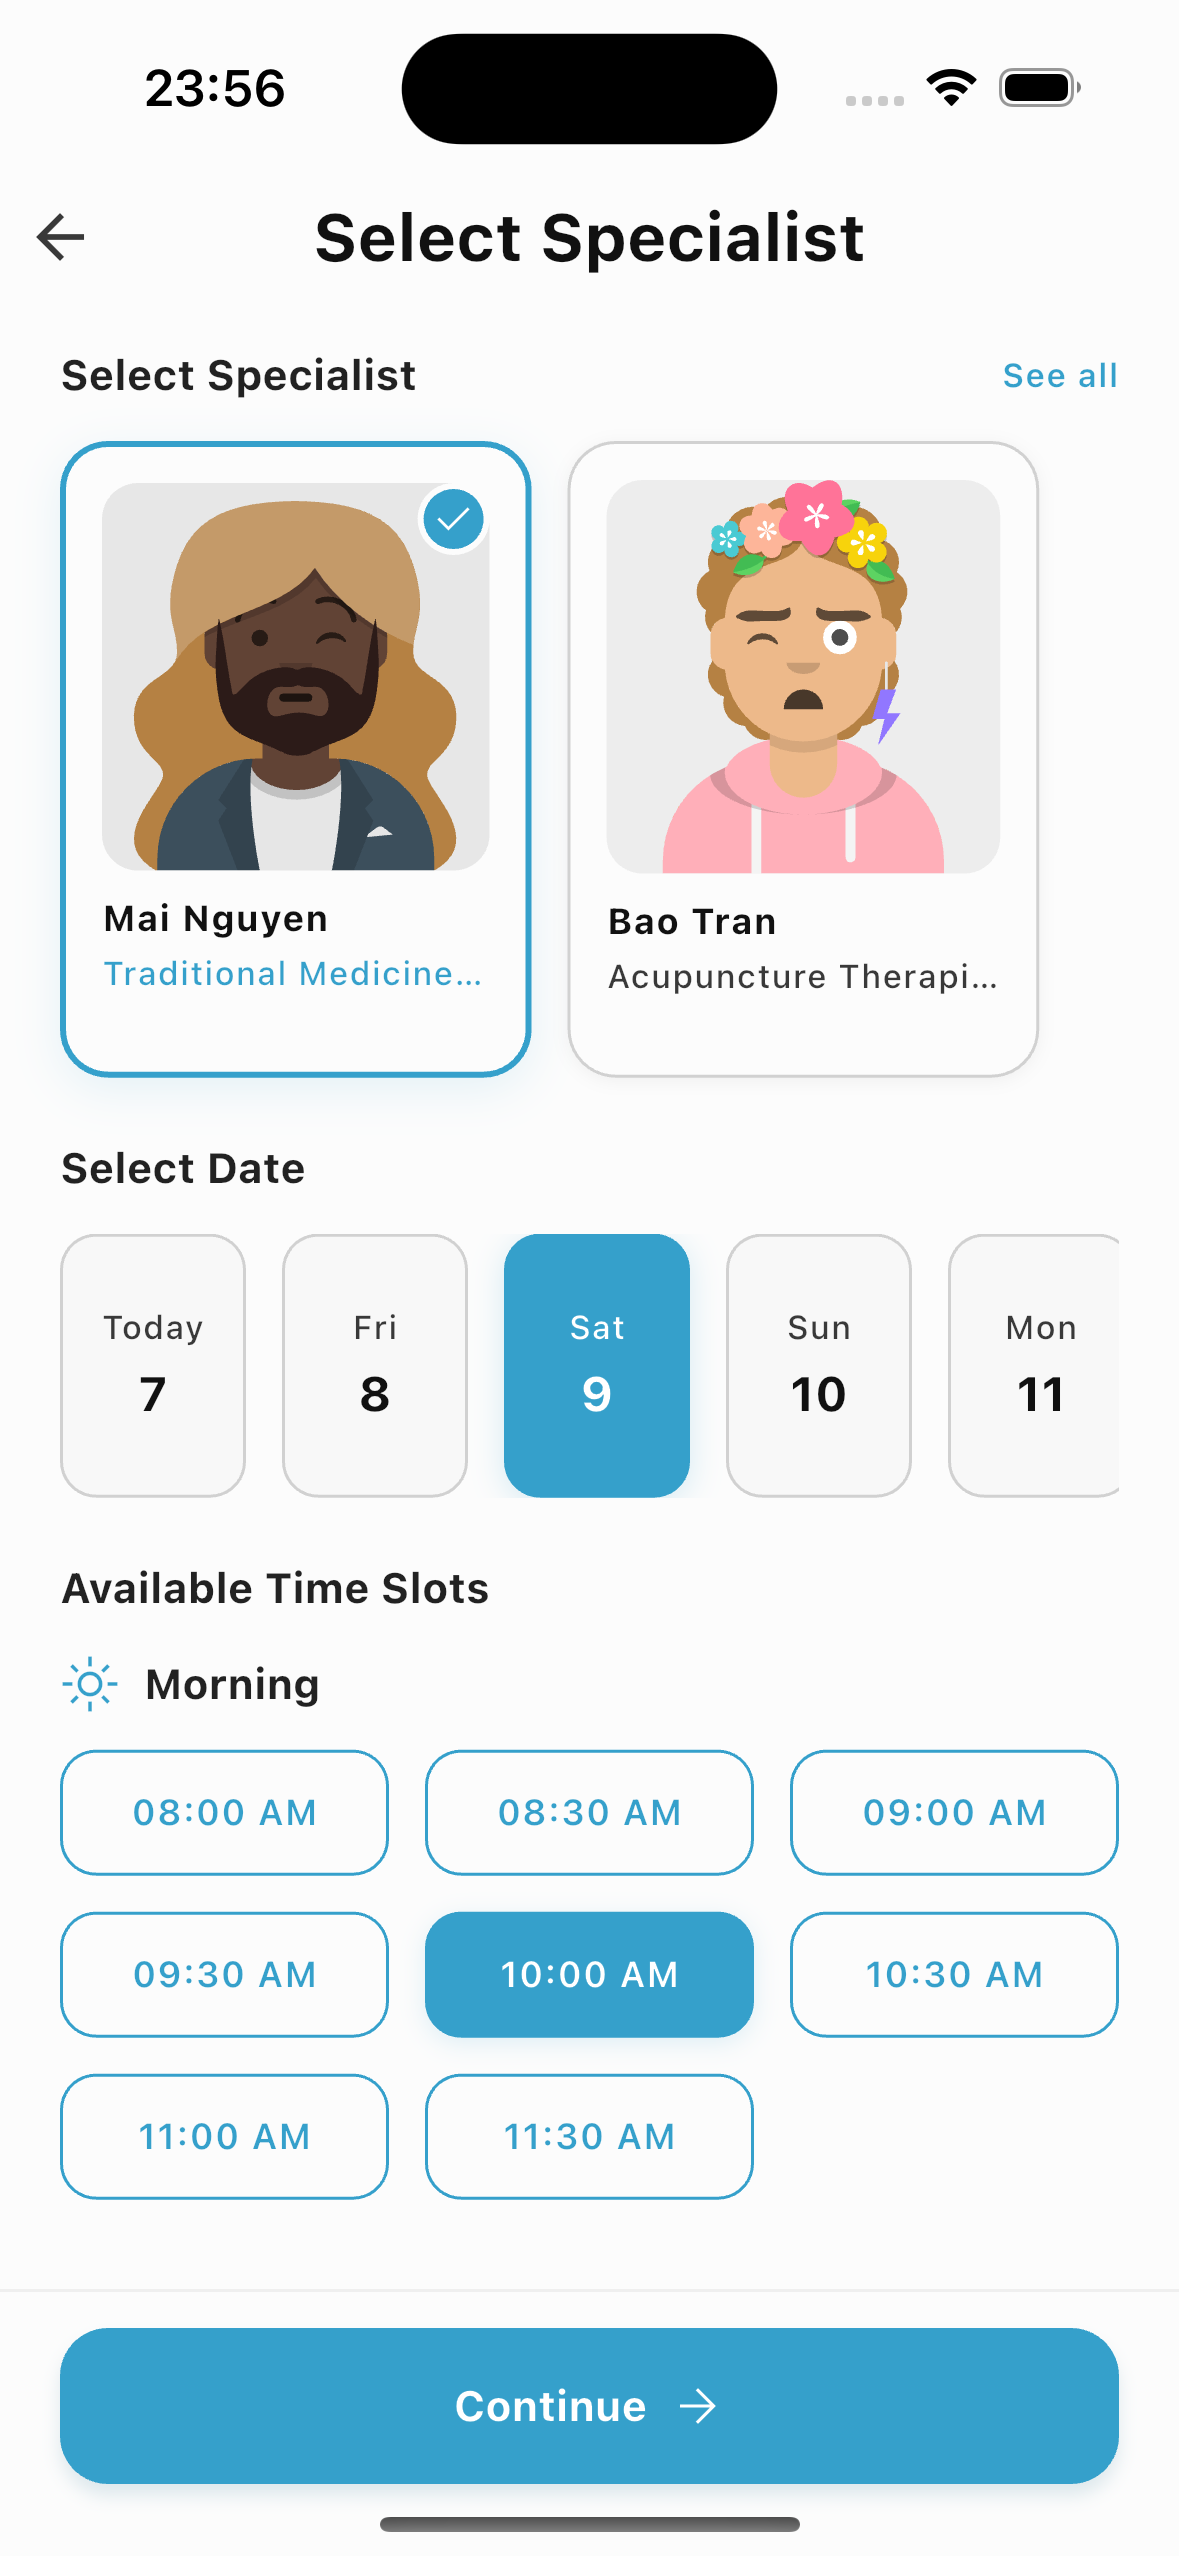
\includegraphics[width=\linewidth,height=0.4\textheight,keepaspectratio]{Images/Hiện thực/user_app/service_details/Simulator Screenshot - iPhone 16 - 2026-05-07 at 23.56.18.png}
    \caption{Chọn chuyên gia và khung giờ}
    \label{fig:service_detail_select_specialist}
\end{subfigure}
\par\medskip
\begin{subfigure}[t]{0.48\linewidth}
    \centering
    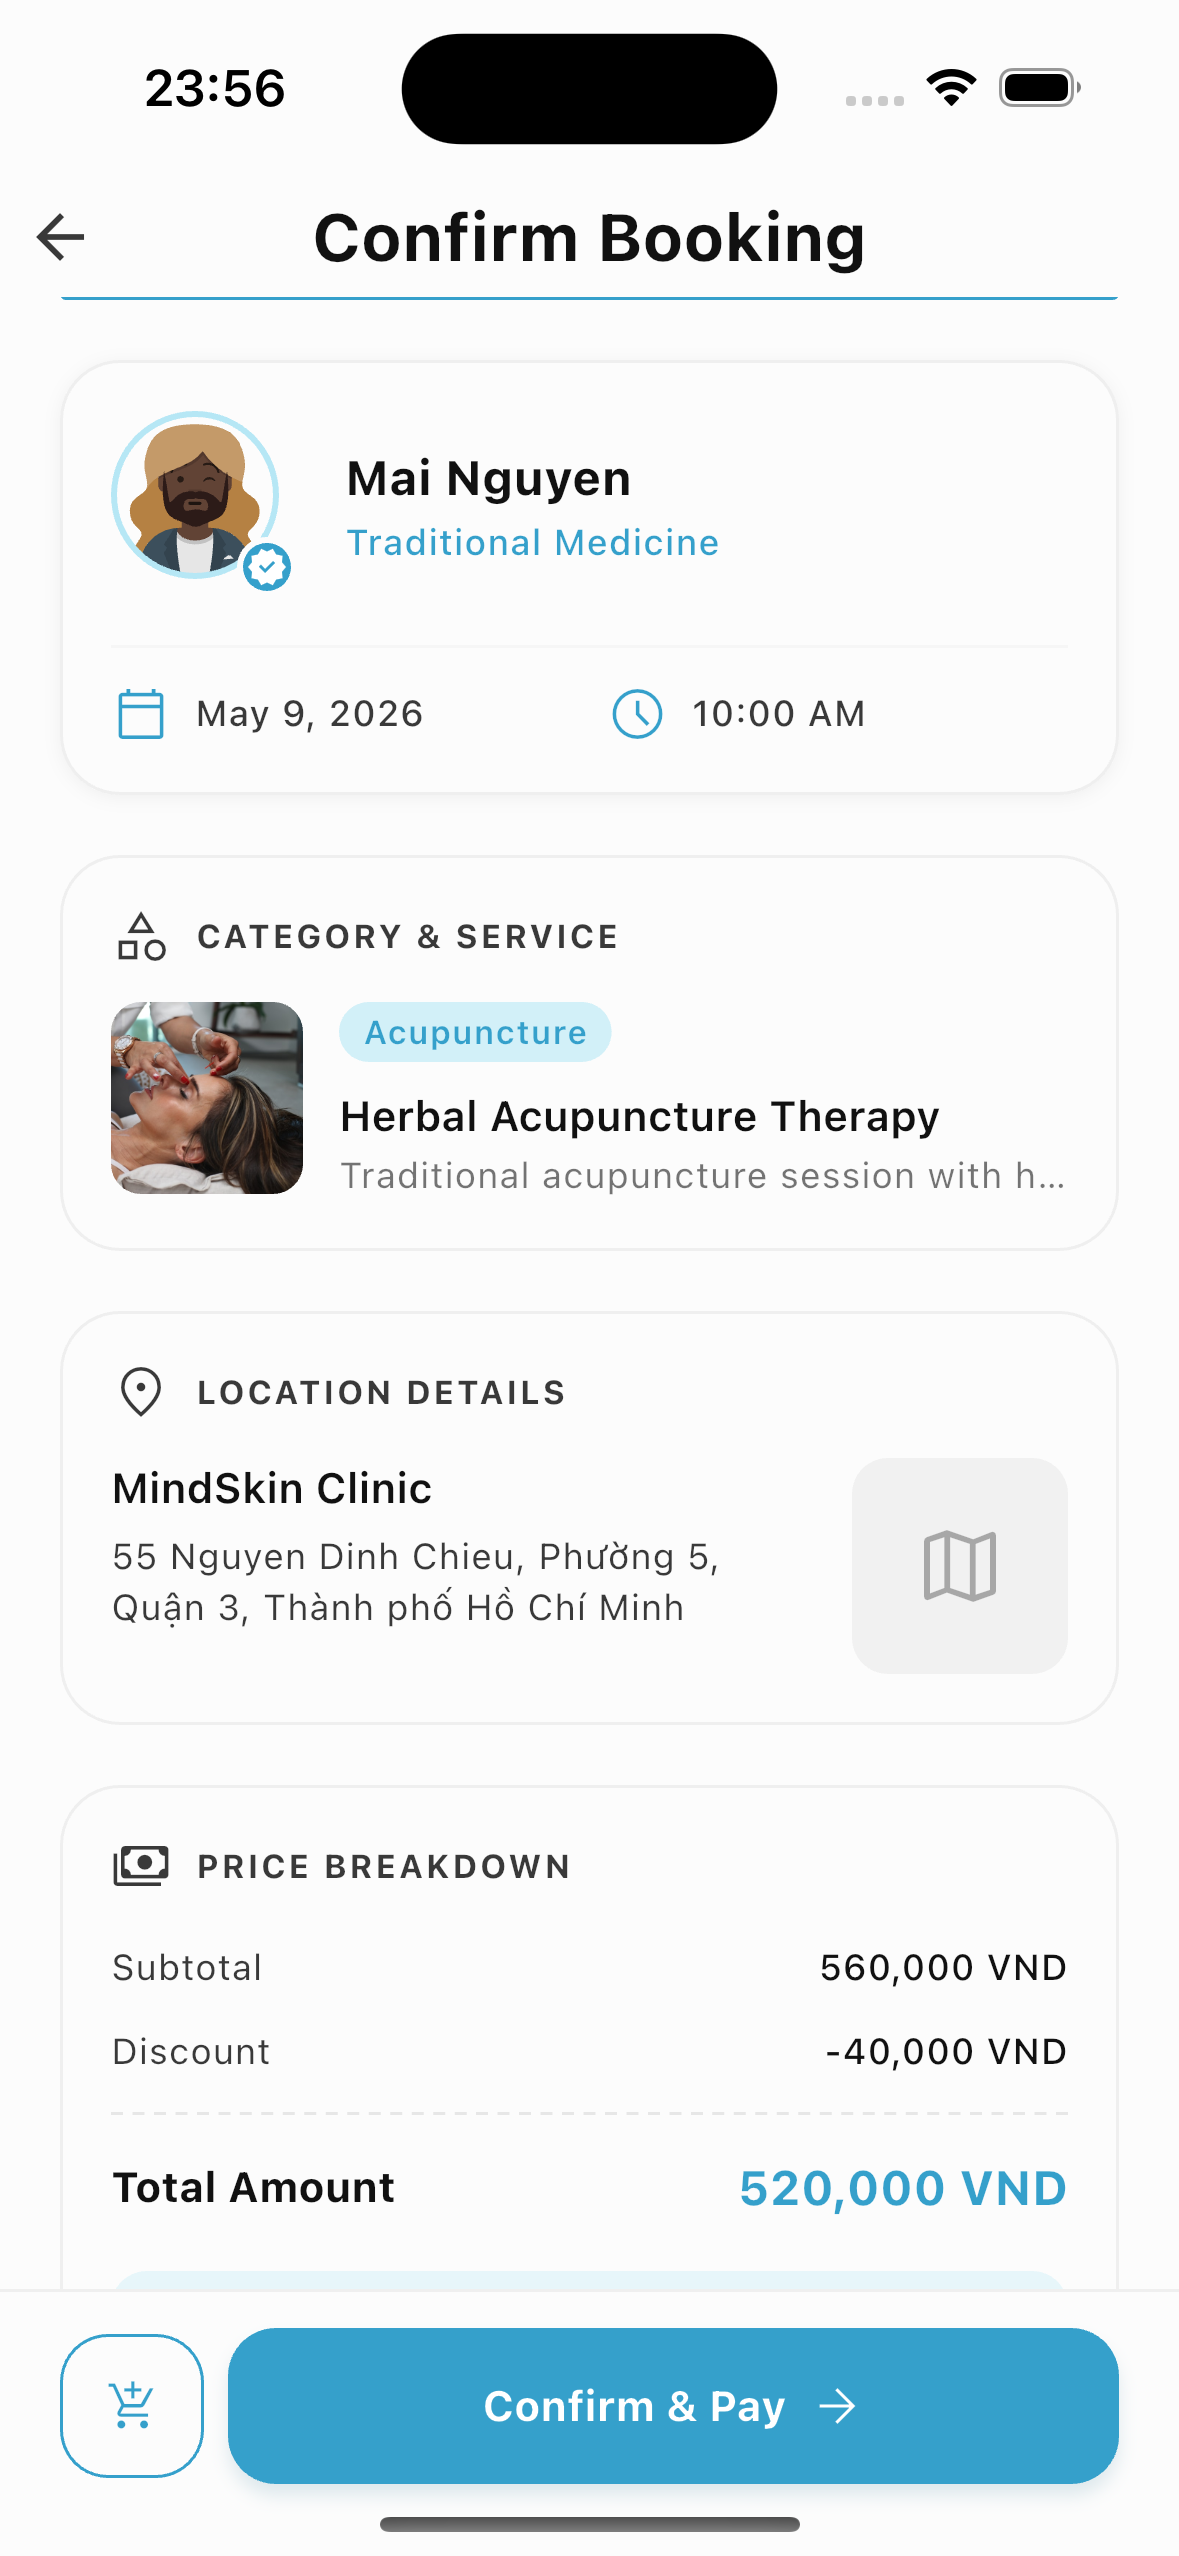
\includegraphics[width=\linewidth,height=0.4\textheight,keepaspectratio]{Images/Hiện thực/user_app/service_details/Simulator Screenshot - iPhone 16 - 2026-05-07 at 23.56.31.png}
    \caption{Xác nhận đặt lịch}
    \label{fig:service_detail_confirm}
\end{subfigure}
\par\medskip
\caption{Luồng đặt lịch dịch vụ trên ứng dụng người dùng}
\label{fig:user_service_booking_flow}
\end{figure}

\begin{itemize}
    \item \textbf{Thao tác xem thông tin:} Người dùng xem ảnh bìa, nhãn dịch vụ, giá, mô tả ngắn và các đánh giá để đánh giá nhanh chất lượng dịch vụ.
    \item \textbf{Thao tác đặt lịch:} Người dùng kéo xuống phần đánh giá, chọn chuyên gia, chọn ngày giờ phù hợp rồi chuyển sang màn hình xác nhận đặt lịch.
\end{itemize}

\subsubsection{Kiến trúc dữ liệu và API}

\paragraph{API Endpoints chính}

\begin{table}[H]
\centering
\begin{tabularx}{\linewidth}{|l|X|X|}
\hline
\textbf{Endpoint} & \textbf{Phương thức} & \textbf{Mô tả} \\
\hline
\texttt{/v1/services} & GET & Lấy danh sách dịch vụ \\
\hline
\texttt{/v1/appointments} & GET & Danh sách lịch hẹn \\
\hline
\texttt{/v1/appointments} & POST & Tạo lịch hẹn mới \\
\hline
\texttt{/v1/payments} & POST & Khởi tạo thanh toán \\
\hline
\texttt{/v1/ai/chat} & POST & Chat với AI \\
\hline
\end{tabularx}
\caption{Danh sách API endpoints chính}
\label{tab:user_api_endpoints}
\end{table}

\subsubsection{Quy trình xử lý nghiệp vụ}

\paragraph{Quy trình đặt lịch hẹn}

\begin{enumerate}
    \item Người dùng chọn dịch vụ
    \item Backend lấy slot khả dụng từ lịch làm việc chuyên gia
    \item Sử dụng Redis Redlock ngăn chặn race condition
    \item Tạo draft order với TTL 10 phút
    \item Thanh toán và xác nhận appointment
\end{enumerate}

\subsubsection{Tối ưu hóa hiệu năng}

\begin{itemize}
    \item \textbf{Caching:} Service cache 24 giờ, User cache 1 giờ
    \item \textbf{CDN:} Hình ảnh trên CloudFront/Cloudflare
    \item \textbf{Image Compression:} 80\% quality, 300-500KB per image
    \item \textbf{Lazy Loading:} Render khi scroll tới
    \item \textbf{Code Splitting:} Lazy-load screens không cần thiết
\end{itemize}


% ===========================================================================
% 6.3.3  PHÂN HỆ CỔNG ĐỐI TÁC (PARTNER PORTAL)
% ===========================================================================
\subsection{Hiện thực Phân hệ Cổng Đối tác (Partner Portal)}

Phân hệ Cổng Đối tác hỗ trợ nhà cung cấp quản lý toàn bộ vòng đời vận hành: từ đăng ký và xét duyệt hồ sơ pháp lý, hoàn thiện hồ sơ công khai, quản trị dịch vụ và nhân sự, đến xử lý lịch hẹn và theo dõi chỉ số kinh doanh.

\paragraph{Xử lý phía Backend khi đăng ký}

Khi đối tác nhấn \textbf{``Complete Registration''}, hệ thống thực hiện các bước sau trong cùng một giao dịch (transaction) để đảm bảo tính toàn vẹn dữ liệu:

\begin{enumerate}
    \item \textbf{Kiểm tra trùng lặp:} Đảm bảo email và mã số thuế chưa có trong hệ thống.
    \item \textbf{Kiểm tra địa chỉ:} Xác nhận thông tin tỉnh/huyện/xã hợp lệ thông qua \texttt{LocationsService}.
    \item \textbf{Khởi tạo dữ liệu:} Khởi tạo thông tin tài khoản, thông tin doanh nghiệp, người đại diện pháp lý, và các giấy tờ KYC ban đầu.
    \item \textbf{Cấp quyền truy cập:} Tạo token truy cập để đối tác có thể đăng nhập ngay.
\end{enumerate}

\begin{figure}[H]
\centering
\begin{subfigure}[b]{0.48\linewidth}
    \centering
    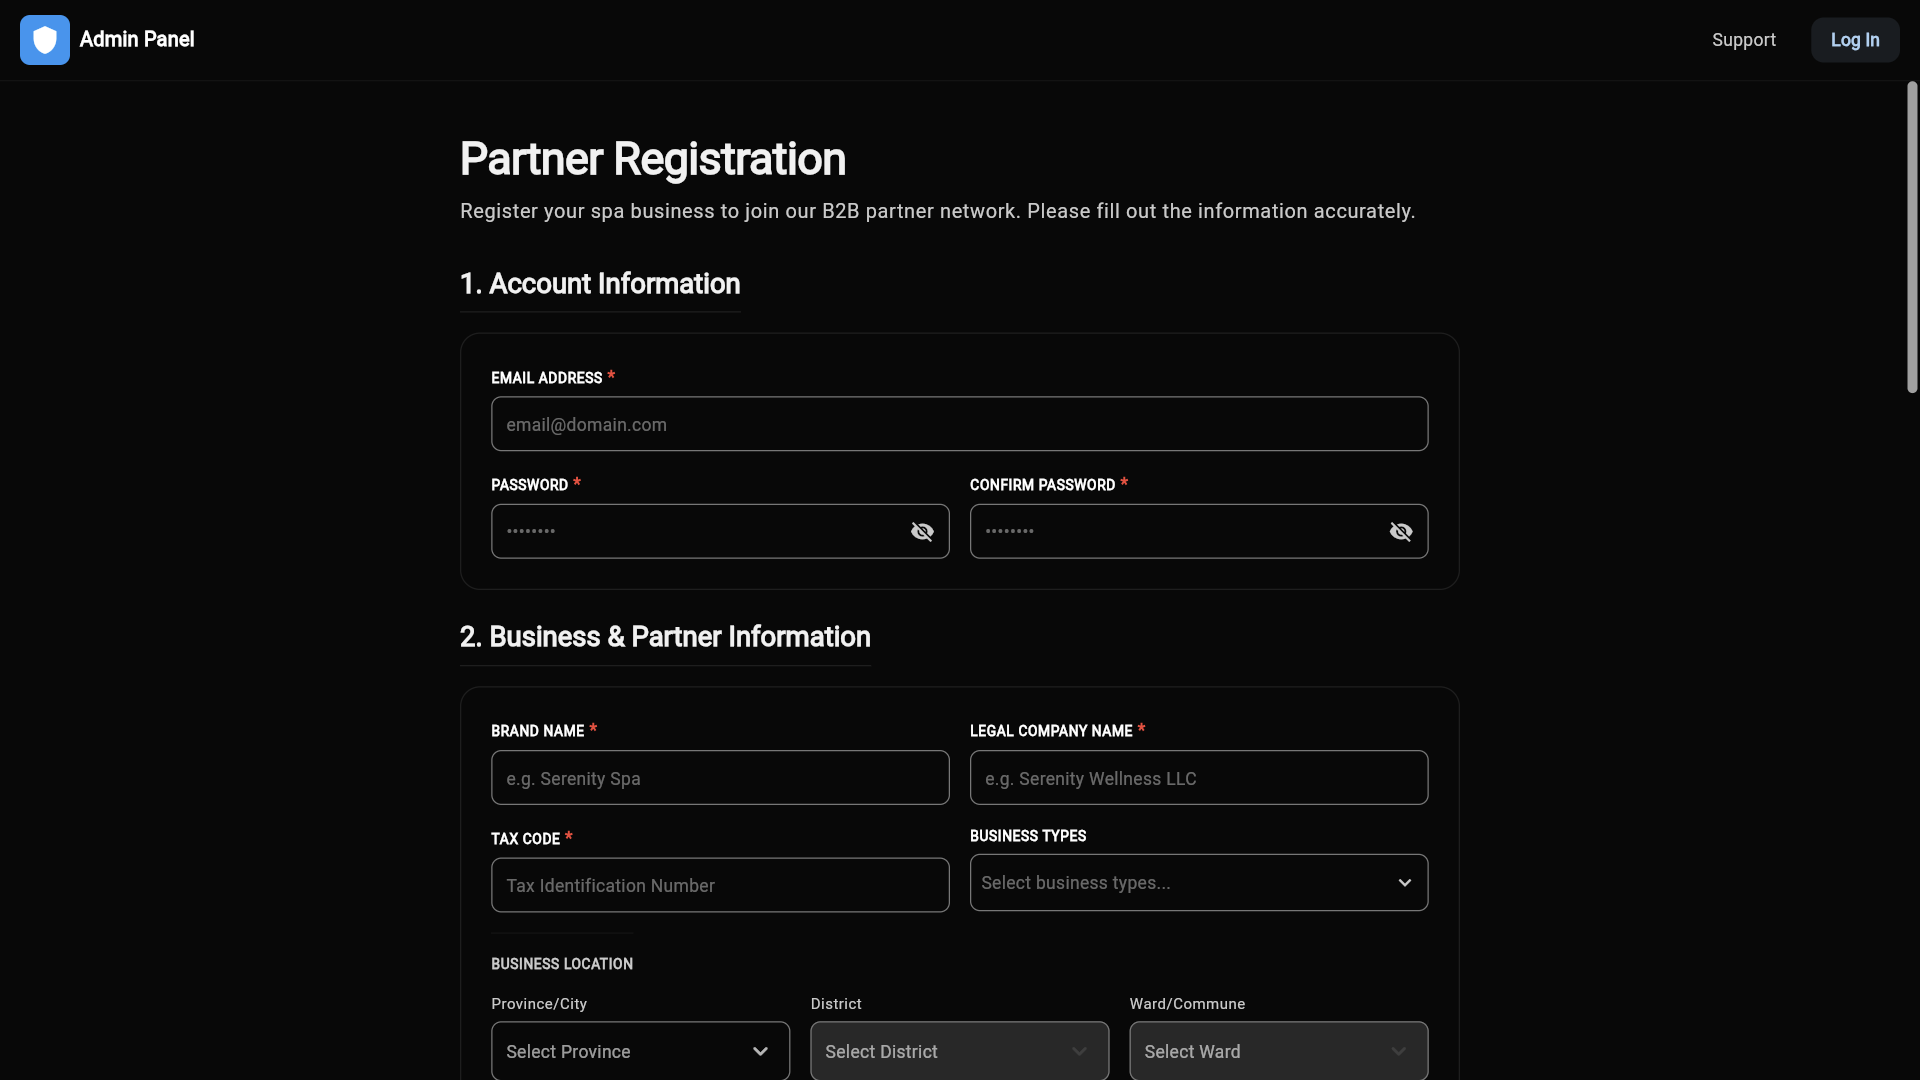
\includegraphics[width=\linewidth]{Images/Hiện thực/partner/fig_partner_reg_account.png}
    \caption{Bước tạo tài khoản đối tác}
    \label{fig:partner_reg_account}
\end{subfigure}
\hfill
\begin{subfigure}[b]{0.48\linewidth}
    \centering
    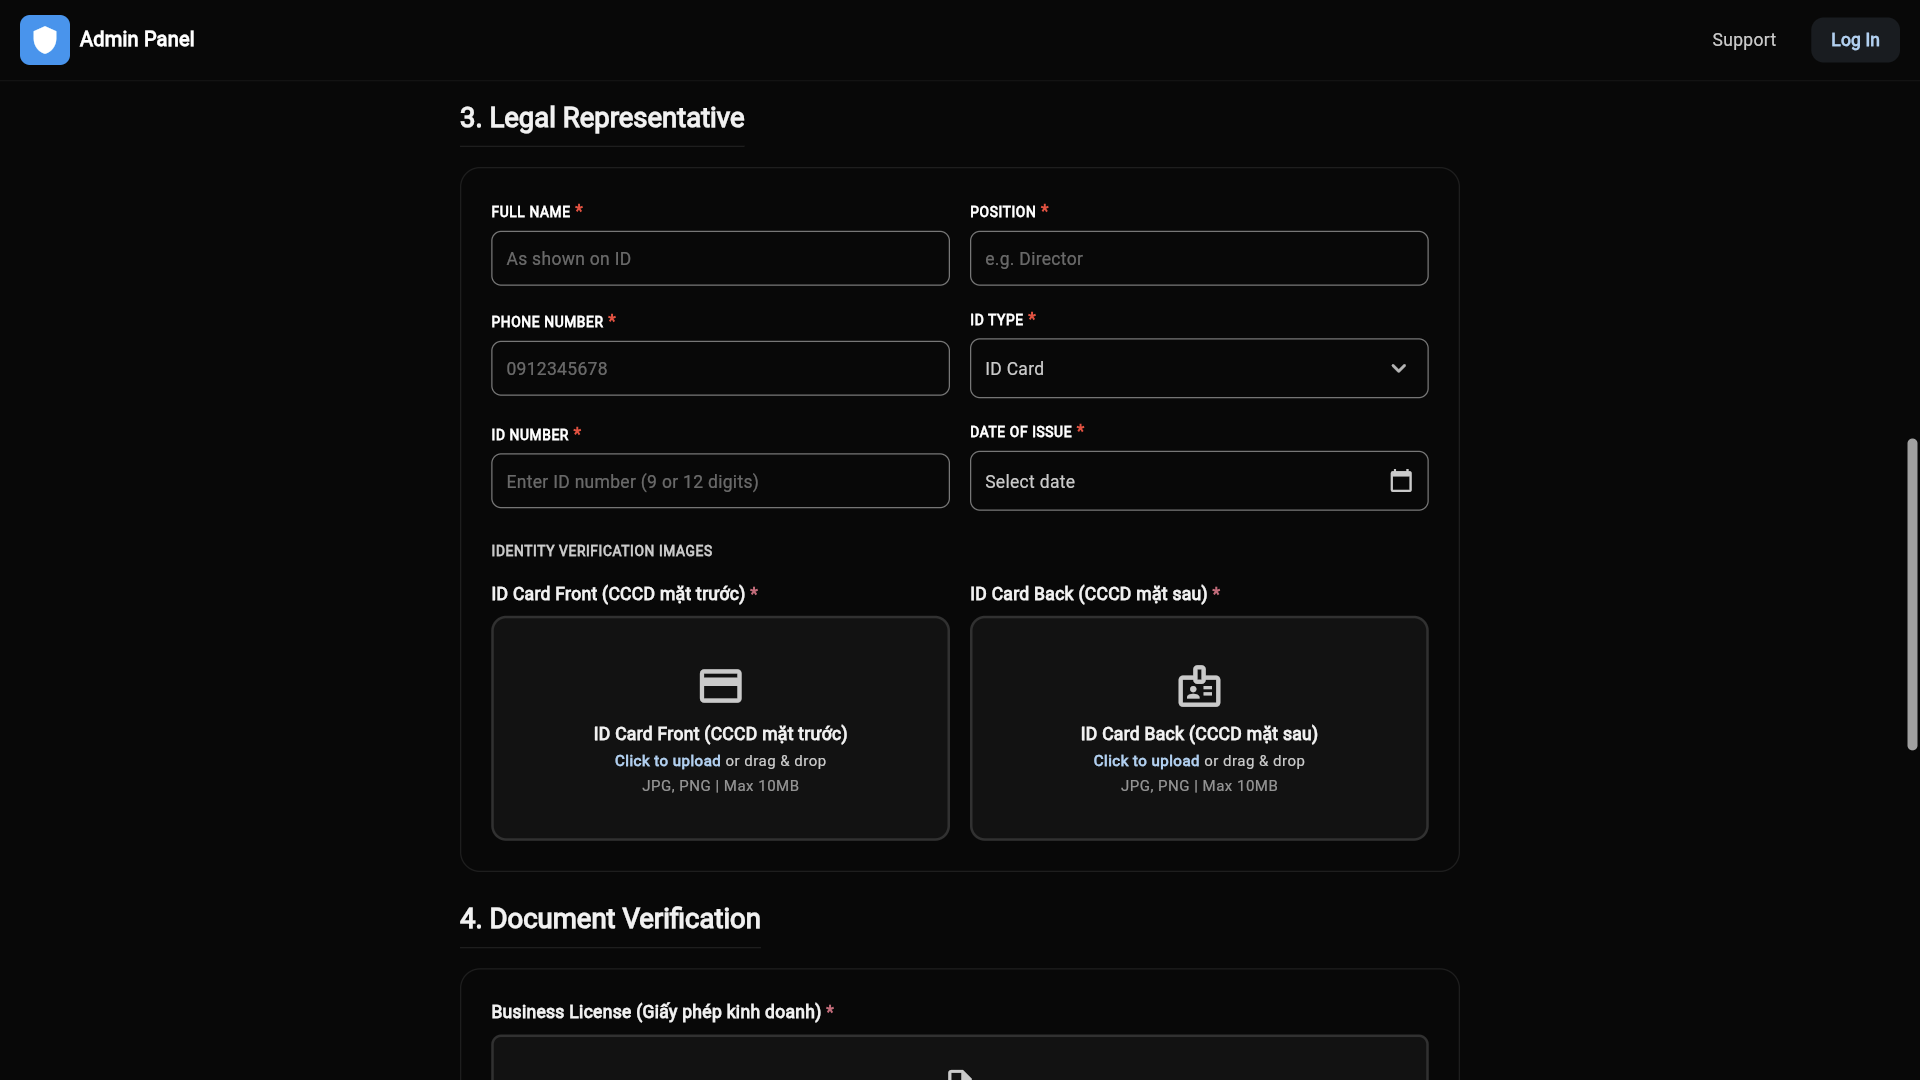
\includegraphics[width=\linewidth]{Images/Hiện thực/partner/fig_partner_reg_legal.png}
    \caption{Khai báo đại diện pháp lý}
    \label{fig:partner_reg_legal}
\end{subfigure}
\par\medskip
\caption{Luồng đăng ký đối tác -- giai đoạn tài khoản và pháp lý}
\end{figure}

\begin{itemize}
    \item \textbf{Thao tác tạo tài khoản:} Đối tác nhập thông tin đăng nhập và dữ liệu liên hệ cơ bản.
    \item \textbf{Thao tác khai báo pháp lý:} Đối tác điền thông tin đại diện pháp luật và giấy tờ định danh bắt buộc.
\end{itemize}

\begin{figure}[H]
\centering
\begin{subfigure}[b]{0.48\linewidth}
    \centering
    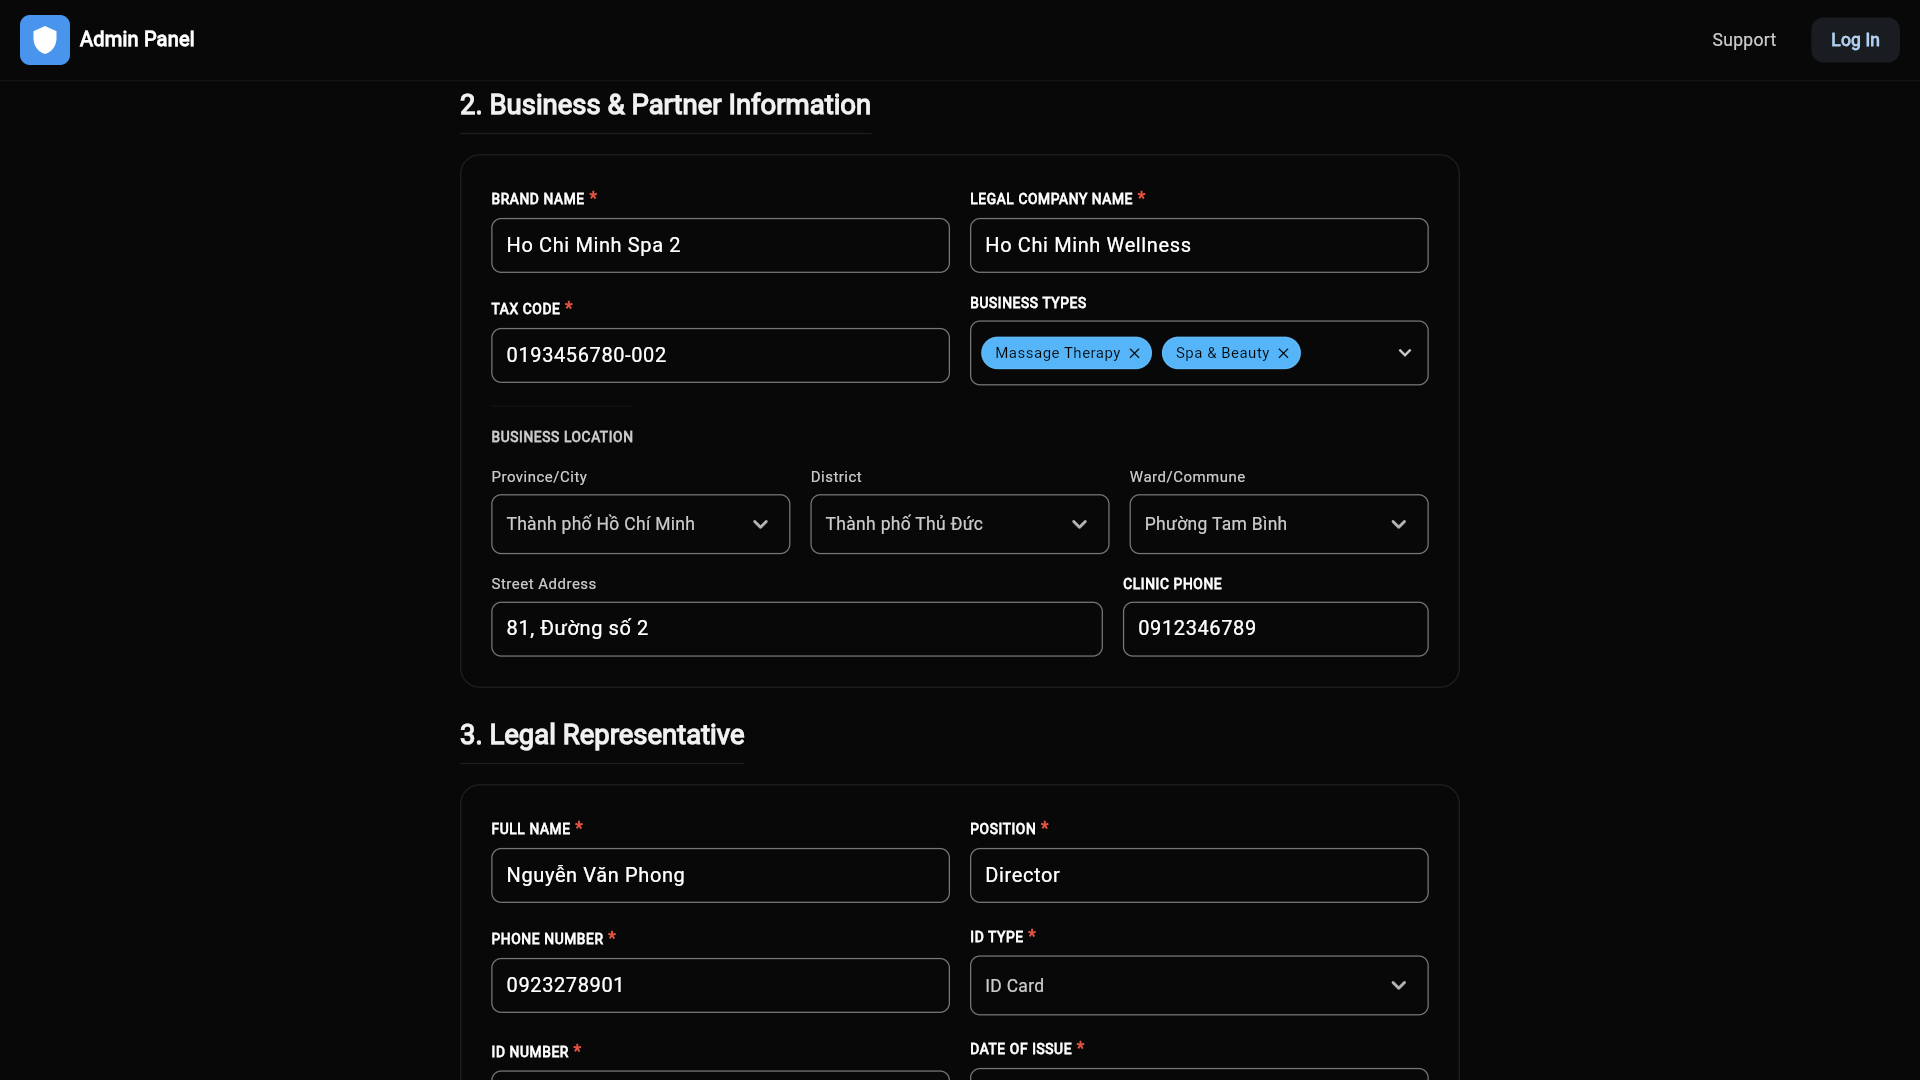
\includegraphics[width=\linewidth]{Images/Hiện thực/partner/fig_partner_reg_filled_business.png}
    \caption{Thông tin doanh nghiệp}
    \label{fig:partner_reg_business}
\end{subfigure}
\hfill
\begin{subfigure}[b]{0.48\linewidth}
    \centering
    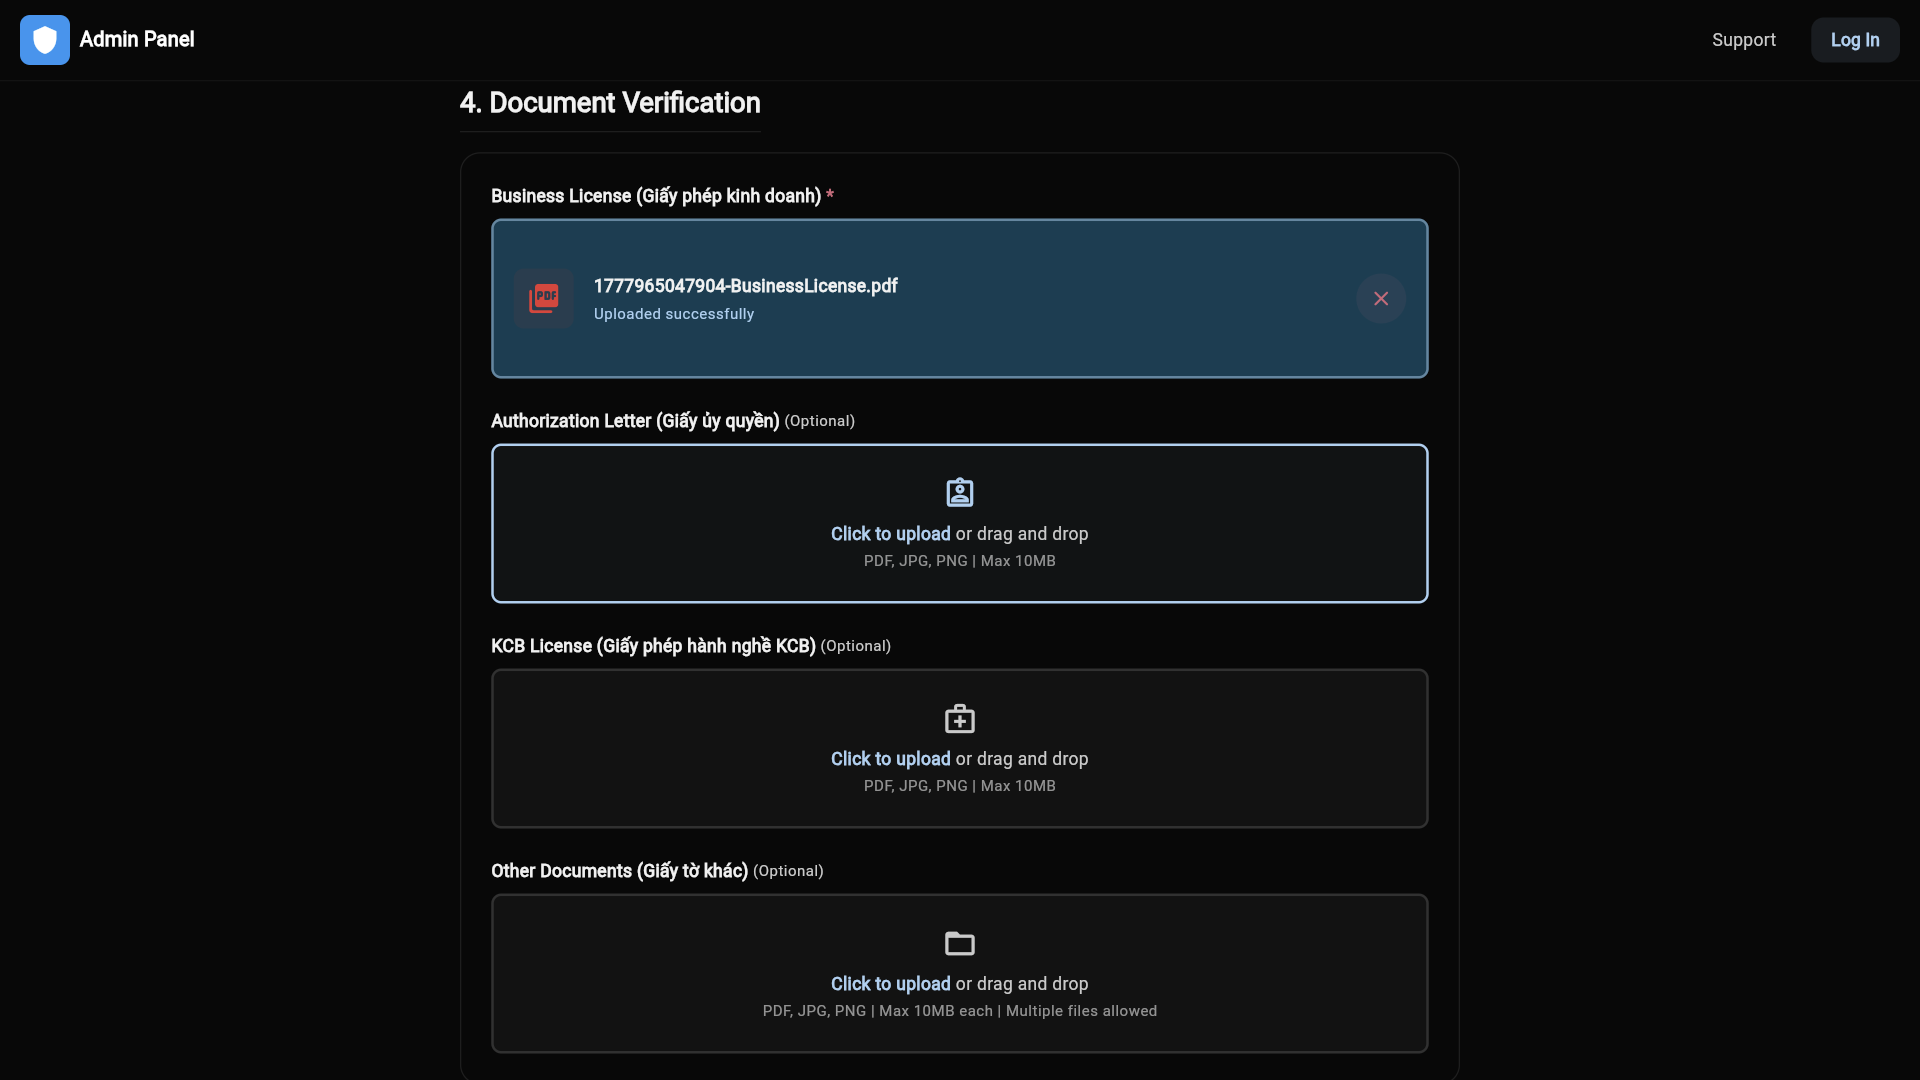
\includegraphics[width=\linewidth]{Images/Hiện thực/partner/fig_partner_reg_doc_uploaded.png}
    \caption{Tải giấy tờ KYC}
    \label{fig:partner_reg_docs}
\end{subfigure}
\par\medskip
\caption{Luồng đăng ký đối tác -- giai đoạn doanh nghiệp và hồ sơ}
\end{figure}

\begin{itemize}
    \item \textbf{Thao tác khai báo doanh nghiệp:} Đối tác điền tên pháp nhân, mã số thuế, địa chỉ và loại hình kinh doanh.
    \item \textbf{Thao tác nộp hồ sơ:} Đối tác tải lên bộ KYC và kiểm tra trạng thái upload trước khi gửi xét duyệt.
\end{itemize}

\begin{figure}[H]
    \centering
    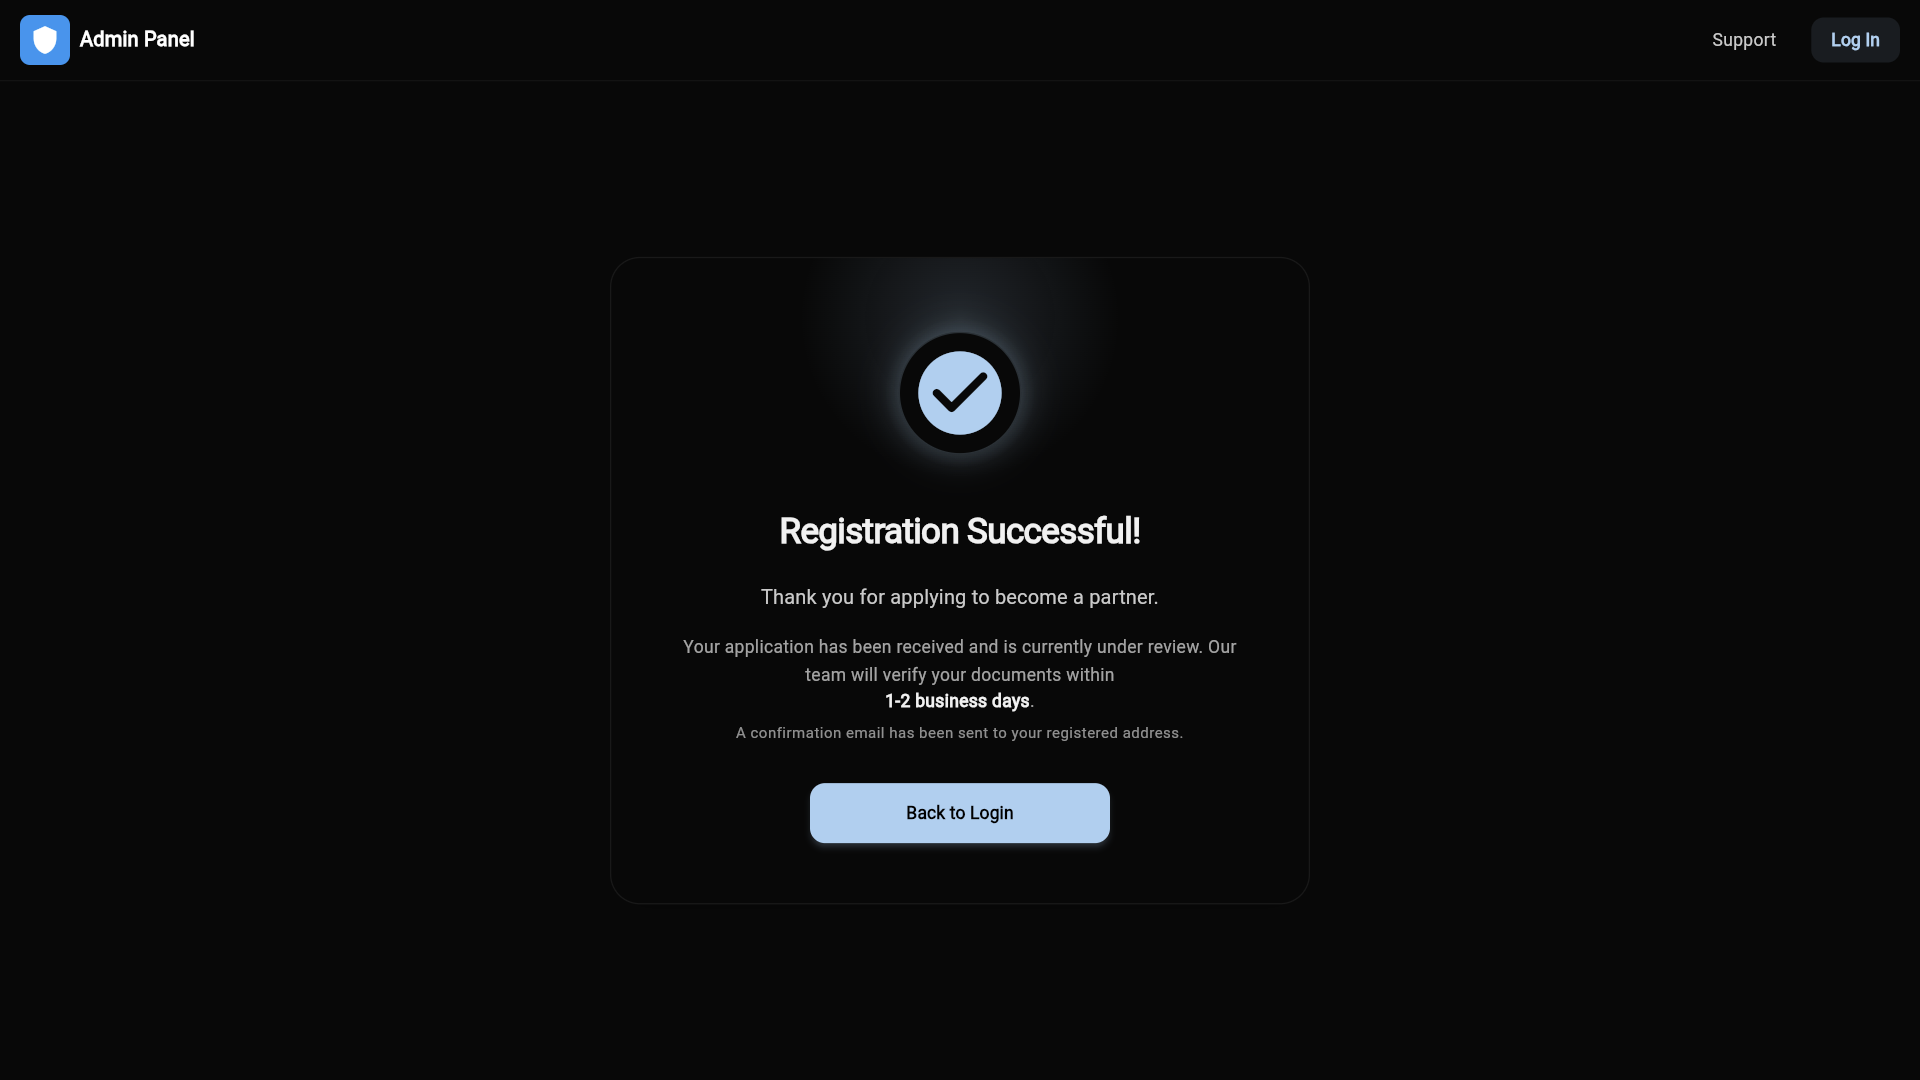
\includegraphics[width=0.85\textwidth]{Images/Hiện thực/partner/fig_partner_reg_success.png}
    \vspace{0.5em}
    \caption{Đăng ký đối tác thành công và chờ xét duyệt}
    \label{fig:partner_reg_success}
\end{figure}

\begin{itemize}
    \item \textbf{Kết quả thao tác:} Hệ thống xác nhận hồ sơ đã gửi thành công và chuyển trạng thái sang \texttt{PENDING}.
    \item \textbf{Bước tiếp theo:} Đối tác theo dõi phản hồi kiểm duyệt hoặc bổ sung hồ sơ khi có yêu cầu chỉnh sửa.
\end{itemize}

Khi đối tác chỉnh sửa hồ sơ (đặc biệt sau khi bị yêu cầu bổ sung), hệ thống áp dụng cơ chế cập nhật thông minh (Smart Update): nhận diện thay đổi qua \texttt{fieldKey}, phân loại mức độ nhạy cảm (mã số thuế, địa chỉ vs. số điện thoại), và tự động chuyển trạng thái phù hợp --- từ \texttt{REQUIRED\_RESUBMIT} về \texttt{PENDING} khi sửa xong lỗi, hoặc thu hồi \texttt{APPROVED} khi sửa thông tin nhạy cảm.

\subsubsection{Hoàn thiện Hồ sơ Công khai (Post-Verification)}

Sau khi được Admin phê duyệt (\texttt{APPROVED}), đối tác đăng nhập vào Partner Portal và được chuyển đến trang ``Complete Clinic Profile'' để hoàn thiện thông tin công khai --- phần dữ liệu sẽ hiển thị cho người dùng cuối trên ứng dụng di động. Quy trình hoàn thiện gồm các bước sau (Hình~\ref{fig:partner_clinic_empty} đến Hình~\ref{fig:partner_clinic_branding}):

\begin{enumerate}
    \item \textbf{Giới thiệu phòng khám (About Clinic):} Nhập mô tả tổng quan về cơ sở, chuyên môn, kinh nghiệm và phương pháp chăm sóc. Hệ thống yêu cầu tối thiểu 120 ký tự và kiểm tra tính sẵn sàng xuất bản.

    \item \textbf{Thư viện ảnh (Clinic Gallery):} Tải lên 3--8 hình ảnh minh họa không gian phòng khám, trang thiết bị, phòng trị liệu, và môi trường phục vụ bệnh nhân. Hỗ trợ sắp xếp thứ tự hiển thị bằng nút mũi tên.

    \item \textbf{Chứng chỉ tin cậy (Trust Badges):} Thêm các chứng nhận, tiêu chuẩn, hoặc giấy phép chuyên môn để tăng độ tin cậy.
\end{enumerate}

Thanh tiến trình ở cuối trang (``Required completion: X/4'') theo dõi số mục bắt buộc đã hoàn thành. Khi đạt 4/4, đối tác có thể nhấn ``Complete profile'' để công khai trang phòng khám.

\begin{figure}[H]
    \centering
    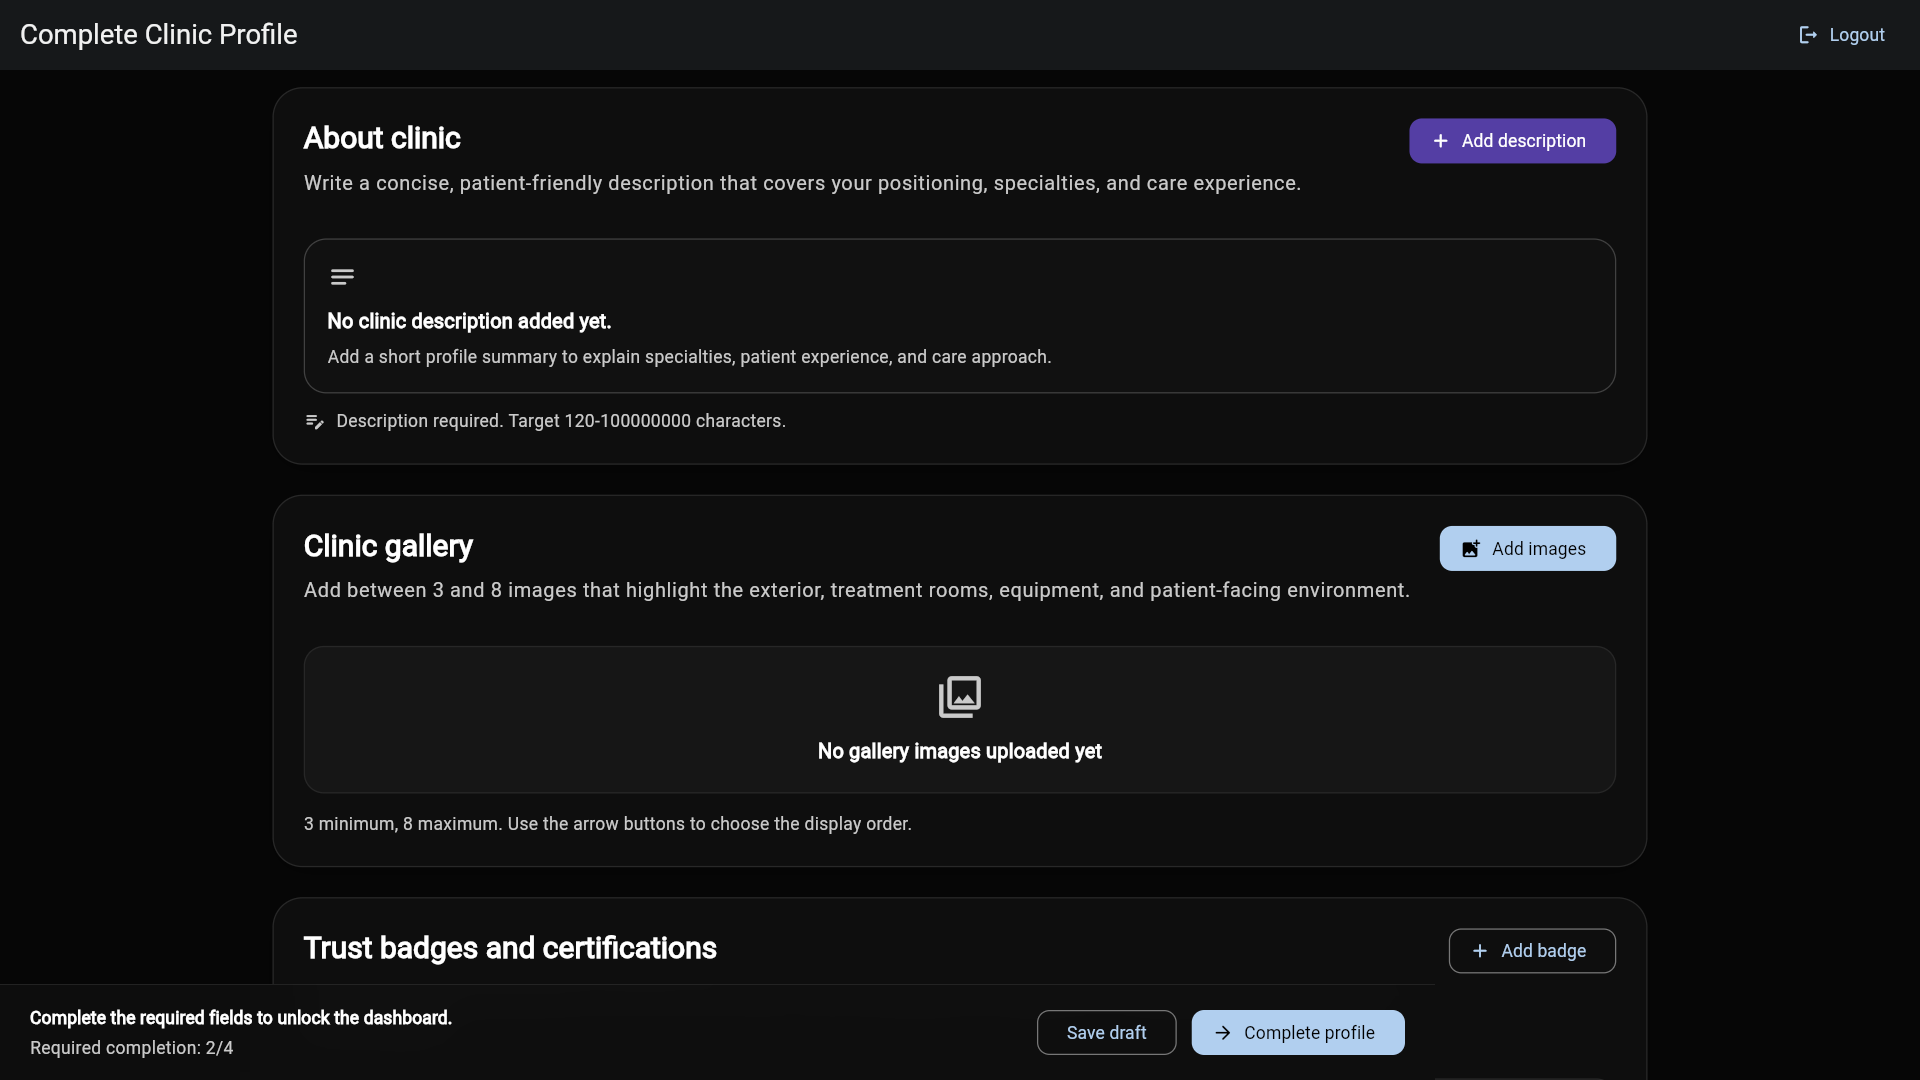
\includegraphics[width=0.92\textwidth]{Images/Hiện thực/partner/fig_partner_clinic_about_empty.png}
    \vspace{1em}
    \caption{Trang hoàn thiện hồ sơ phòng khám -- trạng thái chưa điền}
    \label{fig:partner_clinic_empty}
\end{figure}

\begin{itemize}
    \item \textbf{Trạng thái ban đầu:} Hai mục bắt buộc \textbf{About Clinic} và \textbf{Clinic Gallery} chưa được điền thông tin.
    \item \textbf{Thanh tiến trình (Progress Bar):} Hiển thị ``Required completion: 0/4'', giúp đối tác theo dõi tiến độ hoàn thiện hồ sơ.
\end{itemize}

\begin{figure}[H]
    \centering
    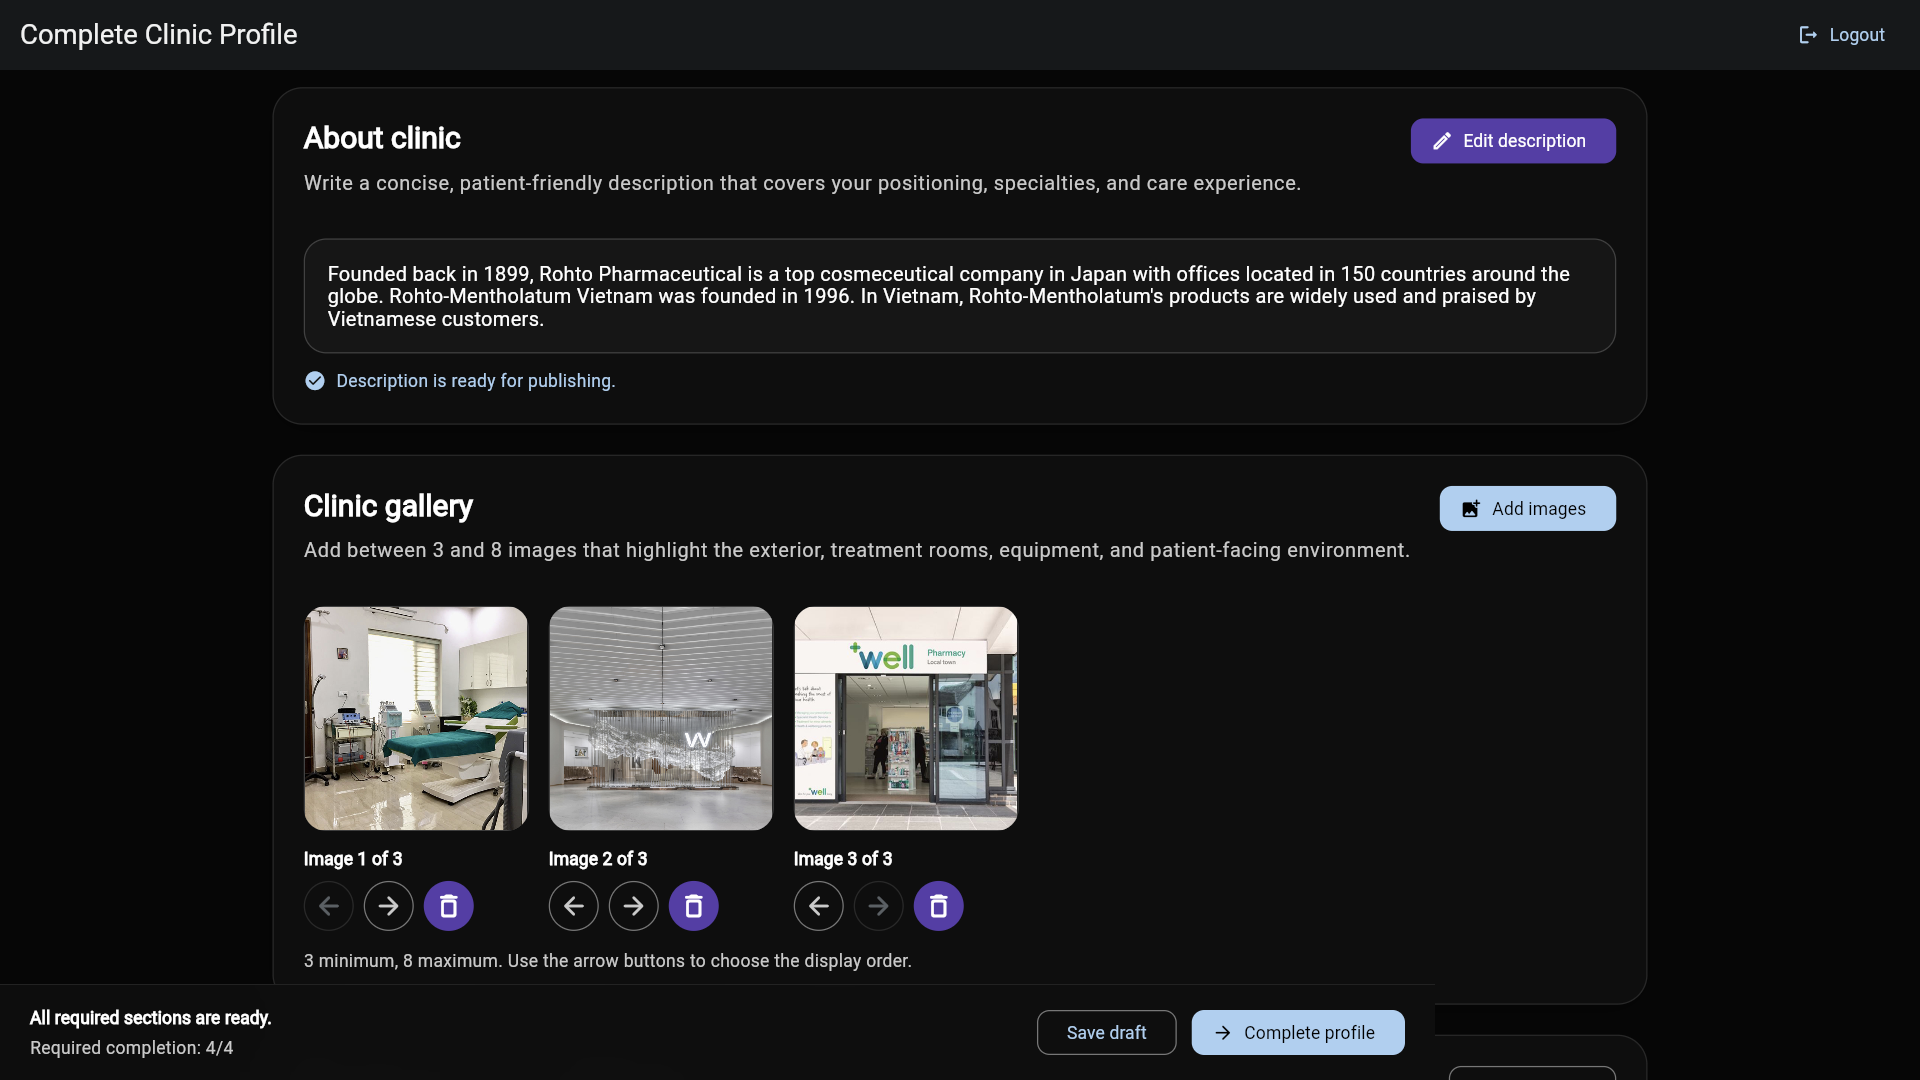
\includegraphics[width=0.92\textwidth]{Images/Hiện thực/partner/fig_partner_clinic_about_filled.png}
    \vspace{1em}
    \caption{Trang hoàn thiện hồ sơ -- đã điền About Clinic và Gallery}
    \label{fig:partner_clinic_filled}
\end{figure}

\begin{itemize}
    \item \textbf{About Clinic:} Nhập mô tả tổng quan về cơ sở (yêu cầu tối thiểu 120 ký tự).
    \item \textbf{Clinic Gallery:} Tải lên hình ảnh minh họa không gian phòng khám, hỗ trợ thao tác sắp xếp thứ tự hiển thị thông qua nút mũi tên lên/xuống.
\end{itemize}

\begin{figure}[H]
    \centering
    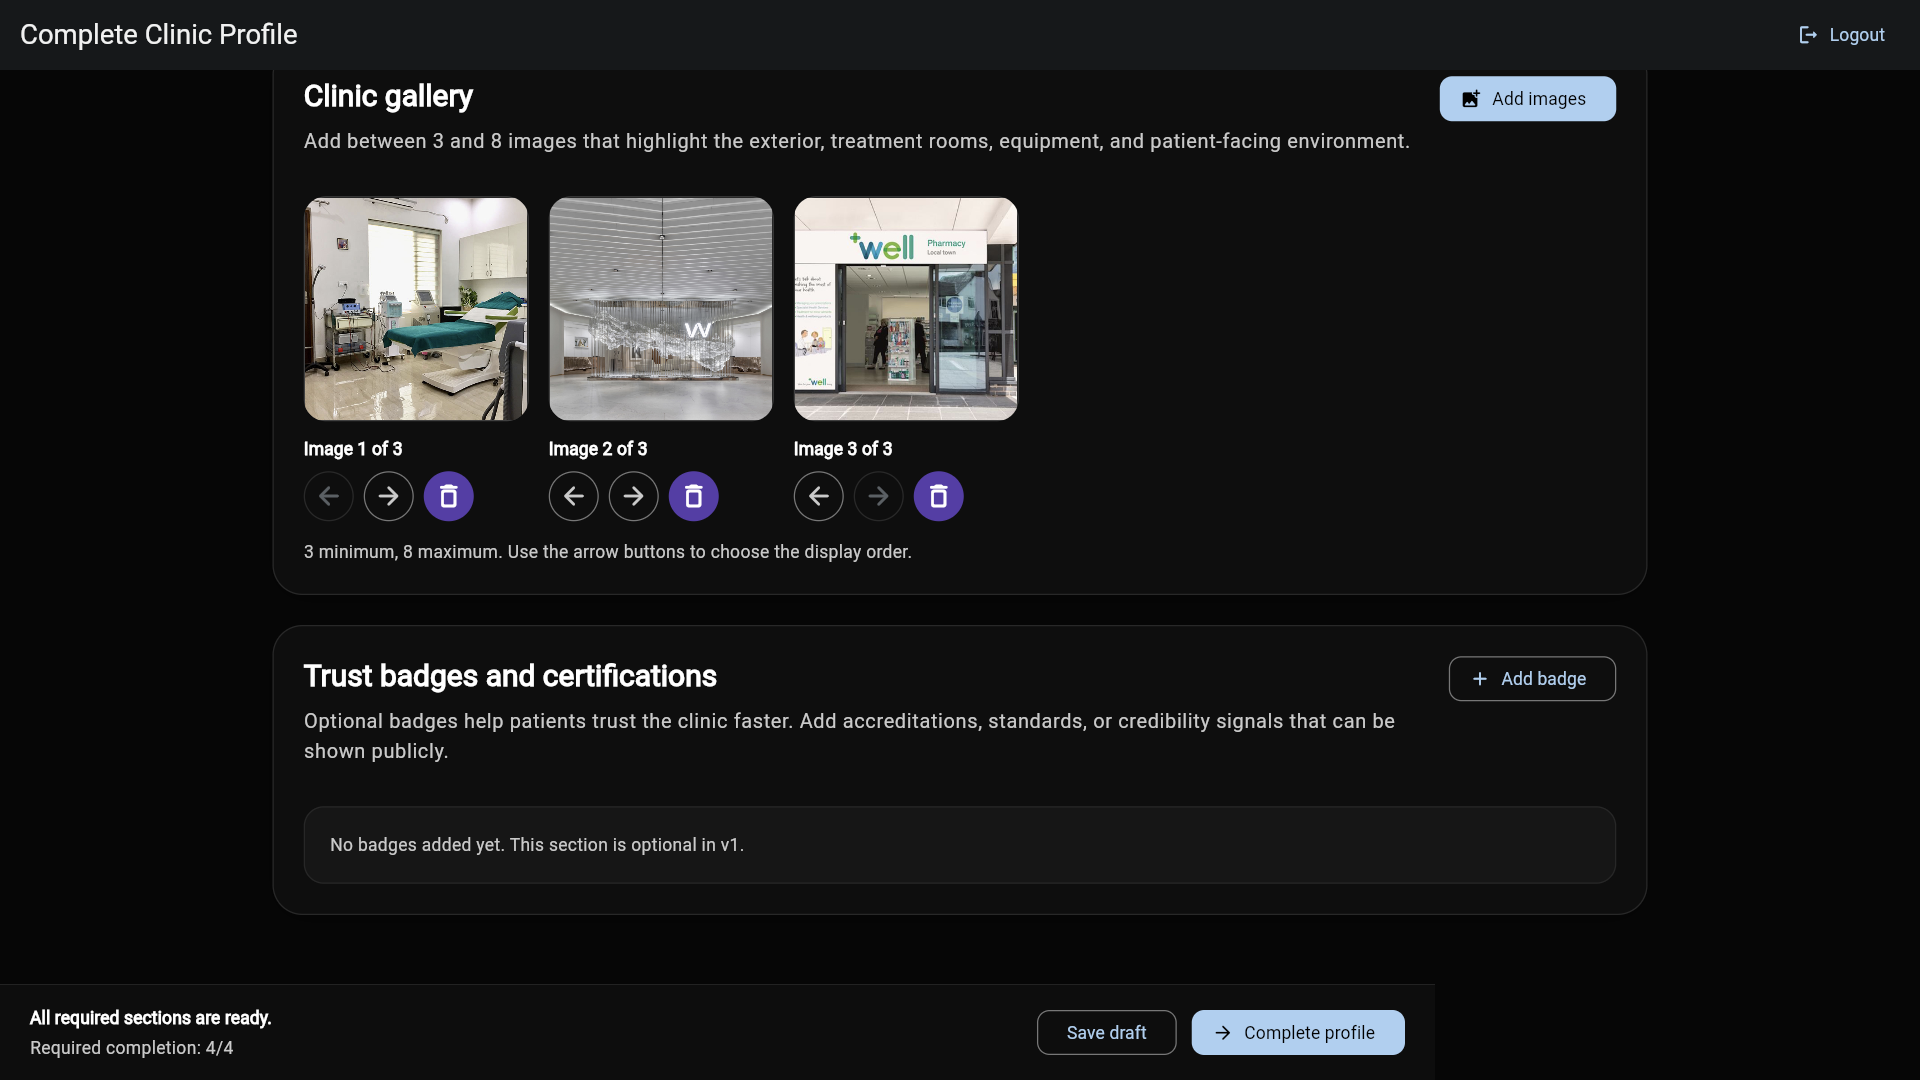
\includegraphics[width=0.92\textwidth]{Images/Hiện thực/partner/fig_partner_clinic_gallery_badges.png}
    \vspace{1em}
    \caption{Phần Trust Badges -- chứng chỉ tin cậy}
    \label{fig:partner_clinic_badges}
\end{figure}

\begin{itemize}
    \item \textbf{Chức năng:} Cho phép đối tác thêm các chứng nhận hoặc giấy phép chuyên môn để tăng độ uy tín.
    \item \textbf{Thông tin mỗi badge:} Bao gồm Title (Tiêu đề), Subtitle (Mô tả phụ), Icon (Biểu tượng), và thứ tự sắp xếp hiển thị.
\end{itemize}

\begin{figure}[H]
    \centering
    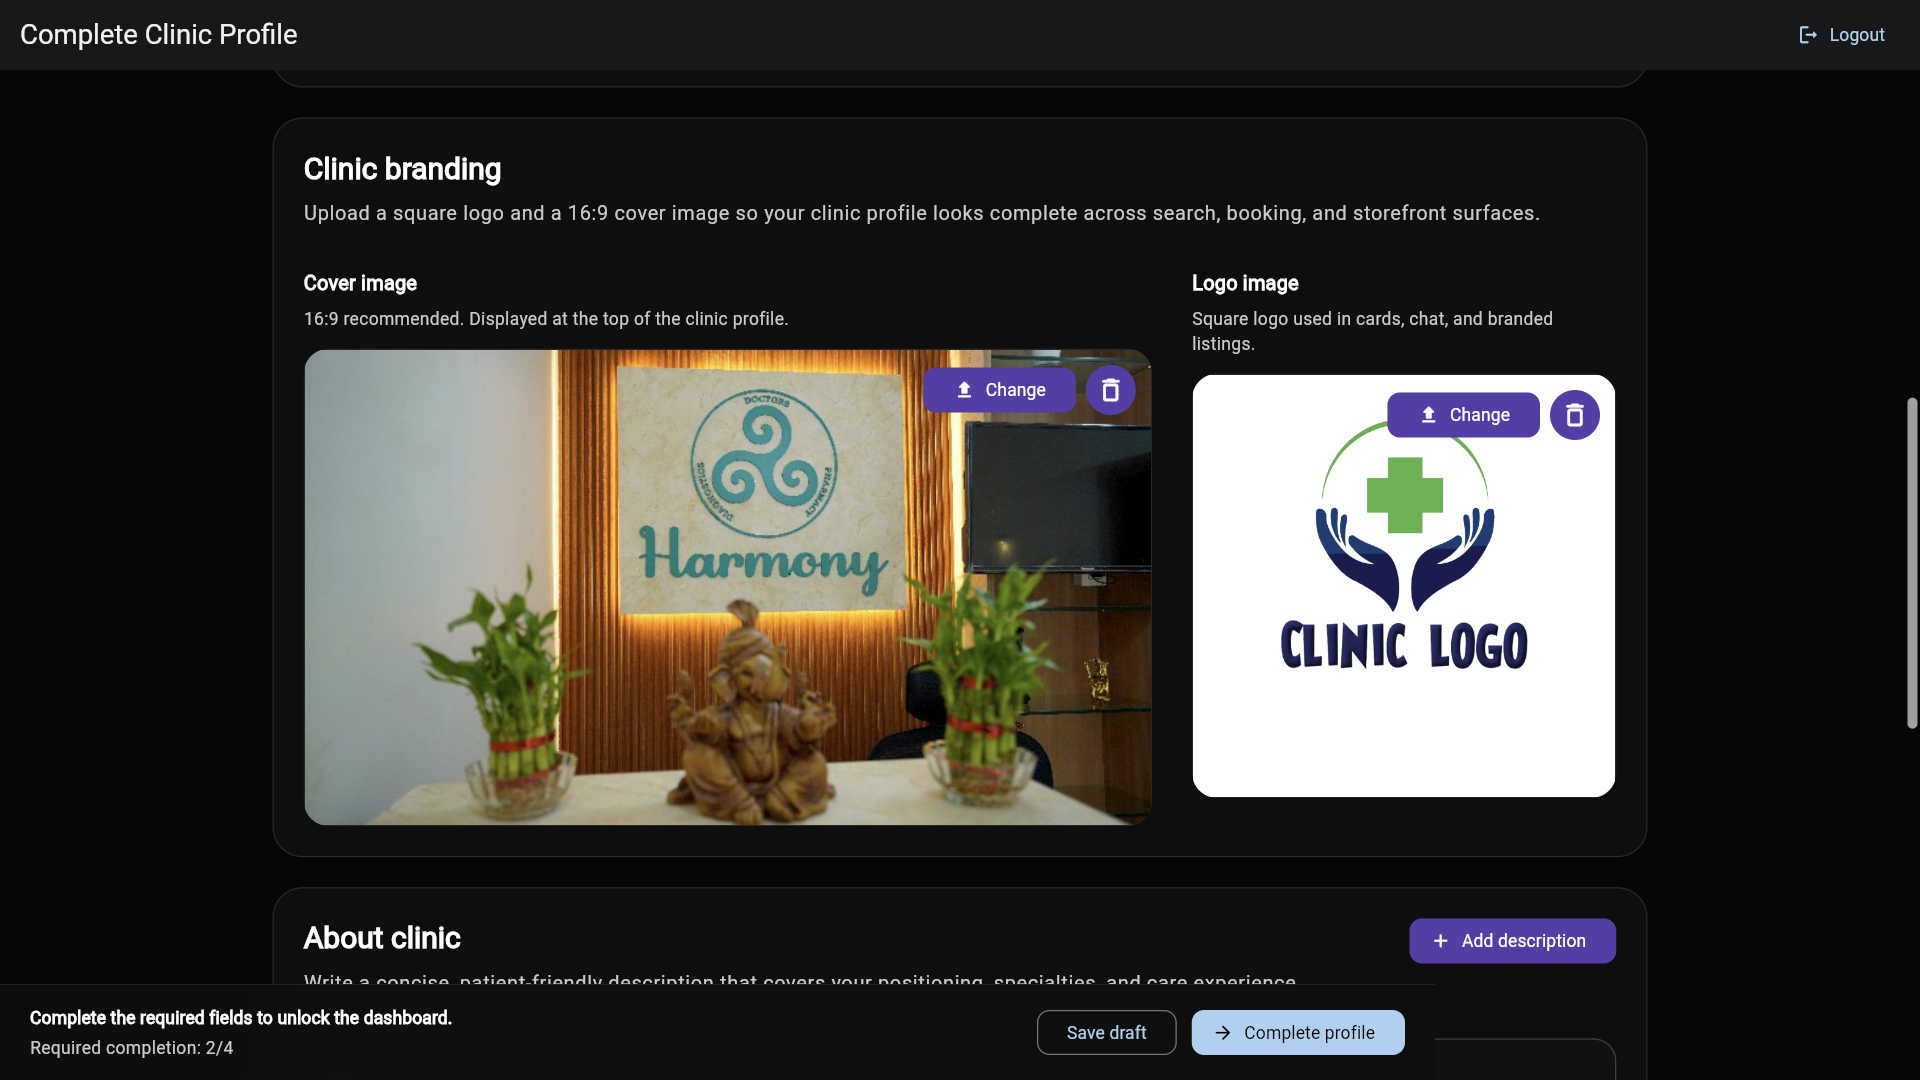
\includegraphics[width=0.92\textwidth]{Images/Hiện thực/partner/fig_partner_clinic_branding_complete.png}
    \vspace{1em}
    \caption{Phần Clinic Branding đã hoàn thiện}
    \label{fig:partner_clinic_branding}
\end{figure}

\begin{itemize}
    \item \textbf{Hình ảnh thương hiệu:} Đối tác đã tải lên ảnh bìa (Cover Image) và logo của phòng khám.
    \item \textbf{Vị trí hiển thị:} Hai hình ảnh này sẽ đóng vai trò nhận diện chính và hiển thị ở vị trí đầu tiên trên trang phòng khám trong ứng dụng di động của người dùng.
\end{itemize}

Dữ liệu từ quy trình này được tổng hợp và hiển thị trên trang chi tiết phòng khám phía người dùng (\texttt{GET /clinics/:id/info}).

\subsubsection{Quản lý Dịch vụ phía Đối tác}

\texttt{PartnerHealthServiceController} (prefix: \texttt{@PartnerApi('health-services')}) cho phép đối tác quản lý dịch vụ của mình:

\begin{itemize}
    \item \textbf{CRUD dịch vụ:} Tạo mới, cập nhật, xóa mềm dịch vụ (Product). Mỗi dịch vụ bao gồm thông tin cơ bản (tên, mô tả, giá gốc, giá khuyến mãi), định nghĩa chi tiết (\texttt{ProductDefinition}: thời lượng phút), và cấu hình hiển thị (\texttt{is\_visible\_online}).
    \item \textbf{Đa phương tiện:} Upload hình ảnh/video qua \texttt{ProductMedia}, hình ảnh cơ sở vật chất qua \texttt{ProductFacilityImage}.
    \item \textbf{Phân công chuyên gia:} Gán nhân viên đủ điều kiện thực hiện dịch vụ qua \texttt{ProductEmployeeEligibility} (quan hệ n-n giữa Product và Employee).
    \item \textbf{Phạm vi truy cập:} Đối tác chỉ được thao tác trên dịch vụ thuộc tổ chức mình. Guard kiểm tra \texttt{partnerId} từ JWT token.
\end{itemize}

Khi dịch vụ được tạo/cập nhật/xóa, hệ thống tự động publish event qua Redis Pub/Sub (\texttt{service:created}, \texttt{service:updated}, \texttt{service:deleted}) để Recommender Service đồng bộ vector store trong thời gian thực.

\subsubsection{Quản lý Nhân sự và Cơ sở}

\paragraph{Module Nhân viên (\texttt{EmployeesModule})}

Quản lý nhân viên, bác sĩ và chuyên gia trên nền tảng:

\begin{itemize}
    \item \texttt{PartnerEmployeesController}: Đối tác CRUD nhân viên, cập nhật lịch làm việc, chuyên môn và trạng thái hoạt động.
    \item \texttt{UserEmployeesController}: Người dùng xem thông tin, tìm kiếm theo chuyên khoa, xem lịch trống.
    \item \textbf{Hồ sơ chuyên biệt:} Mở rộng từ \texttt{Employee} thành \texttt{DoctorProfile} (chuyên khoa, giấy phép hành nghề, \texttt{experience\_years}) và \texttt{TherapistProfile} (phương pháp trị liệu, kinh nghiệm).
\end{itemize}

\paragraph{Module Phòng khám (\texttt{ClinicModule} --- phía Đối tác)}

Quản lý phòng khám và cơ sở dịch vụ: tên, mô tả, hình ảnh, giờ hoạt động. Liên kết \texttt{Address} và tọa độ địa lý (PostGIS) phục vụ tìm kiếm theo vị trí.

\subsubsection{Tiếp nhận Lịch hẹn và Giao tiếp với Khách hàng}

Đối tác tiếp nhận và xử lý lịch hẹn từ khách hàng thông qua giao diện Partner Portal. Khi có booking mới, hệ thống tự động gửi thông báo qua \texttt{NotificationModule}. Đối tác có thể xác nhận hoặc từ chối lịch hẹn, với mọi thay đổi trạng thái được ghi nhận trong \texttt{BookingStatusLog}.

\paragraph{Chat phía Đối tác}

Đối xứng với phía người dùng, đối tác có hệ thống chat riêng:

\begin{itemize}
    \item \textbf{\texttt{PartnerChatController}:} REST API quản lý danh sách cuộc trò chuyện, lịch sử tin nhắn (phân trang), đánh dấu đã đọc, và hỗ trợ tệp đính kèm (\texttt{PartnerChatAttachment}).
    \item \textbf{\texttt{PartnerChatGateway}:} WebSocket Gateway xử lý nhắn tin thời gian thực phía đối tác. Tích hợp \texttt{ChatNotificationGateway} để đẩy thông báo tin nhắn mới khi đối tác không ở trong màn hình chat.
    \item \textbf{Xác thực:} Sử dụng chung middleware \texttt{ws-jwt-auth} với phía người dùng, phân biệt role qua JWT payload.
\end{itemize}

\subsubsection{Dashboard Đối tác (\texttt{DashboardPartnerModule})}

Cung cấp bảng điều khiển phân tích nghiệp vụ cho đối tác thông qua \texttt{PartnerDashboardController}, bao gồm các endpoint:

\begin{itemize}
    \item \textbf{\texttt{GET /stats}:} Thống kê KPI tổng hợp (doanh thu, số booking, tỷ lệ hoàn thành) theo kỳ tuần/tháng/quý.
    \item \textbf{\texttt{GET /revenue}:} Dữ liệu doanh thu time-series phục vụ vẽ biểu đồ xu hướng.
    \item \textbf{\texttt{GET /appointments/upcoming}:} Danh sách lịch hẹn sắp tới cần xử lý.
    \item \textbf{\texttt{GET /services/performance}:} Xếp hạng hiệu suất dịch vụ theo doanh thu và lượt đặt.
    \item \textbf{\texttt{GET /employees/distribution}:} Thống kê phân bố nhân sự theo vai trò.
    \item \textbf{\texttt{GET /reviews/recent}:} Đánh giá gần nhất từ khách hàng.
    \item \textbf{\texttt{GET /staff/schedule}:} Lịch nhân viên theo ngày cụ thể.
    \item \textbf{\texttt{GET /notifications}:} Thông báo và cảnh báo cho đối tác.
    \item \textbf{\texttt{GET /inventory/alerts}:} Cảnh báo về thiết bị hoặc vật tư cần bổ sung.
\end{itemize}

Toàn bộ endpoint bảo vệ bởi \texttt{@PartnerApi} decorator, đảm bảo đối tác chỉ xem dữ liệu thuộc tổ chức mình. Giao diện Dashboard (Hình~\ref{fig:partner_dashboard}) hiển thị tổng quan kinh doanh gồm: (1)~Doanh thu tổng, (2)~Số lịch hẹn, (3)~Dịch vụ đang hoạt động, (4)~Đánh giá trung bình, cùng biểu đồ doanh thu theo thời gian và các thao tác nhanh (Quick Actions) để thêm dịch vụ, nhân viên, hoặc quản lý tin nhắn.

\begin{figure}[H]
    \centering
    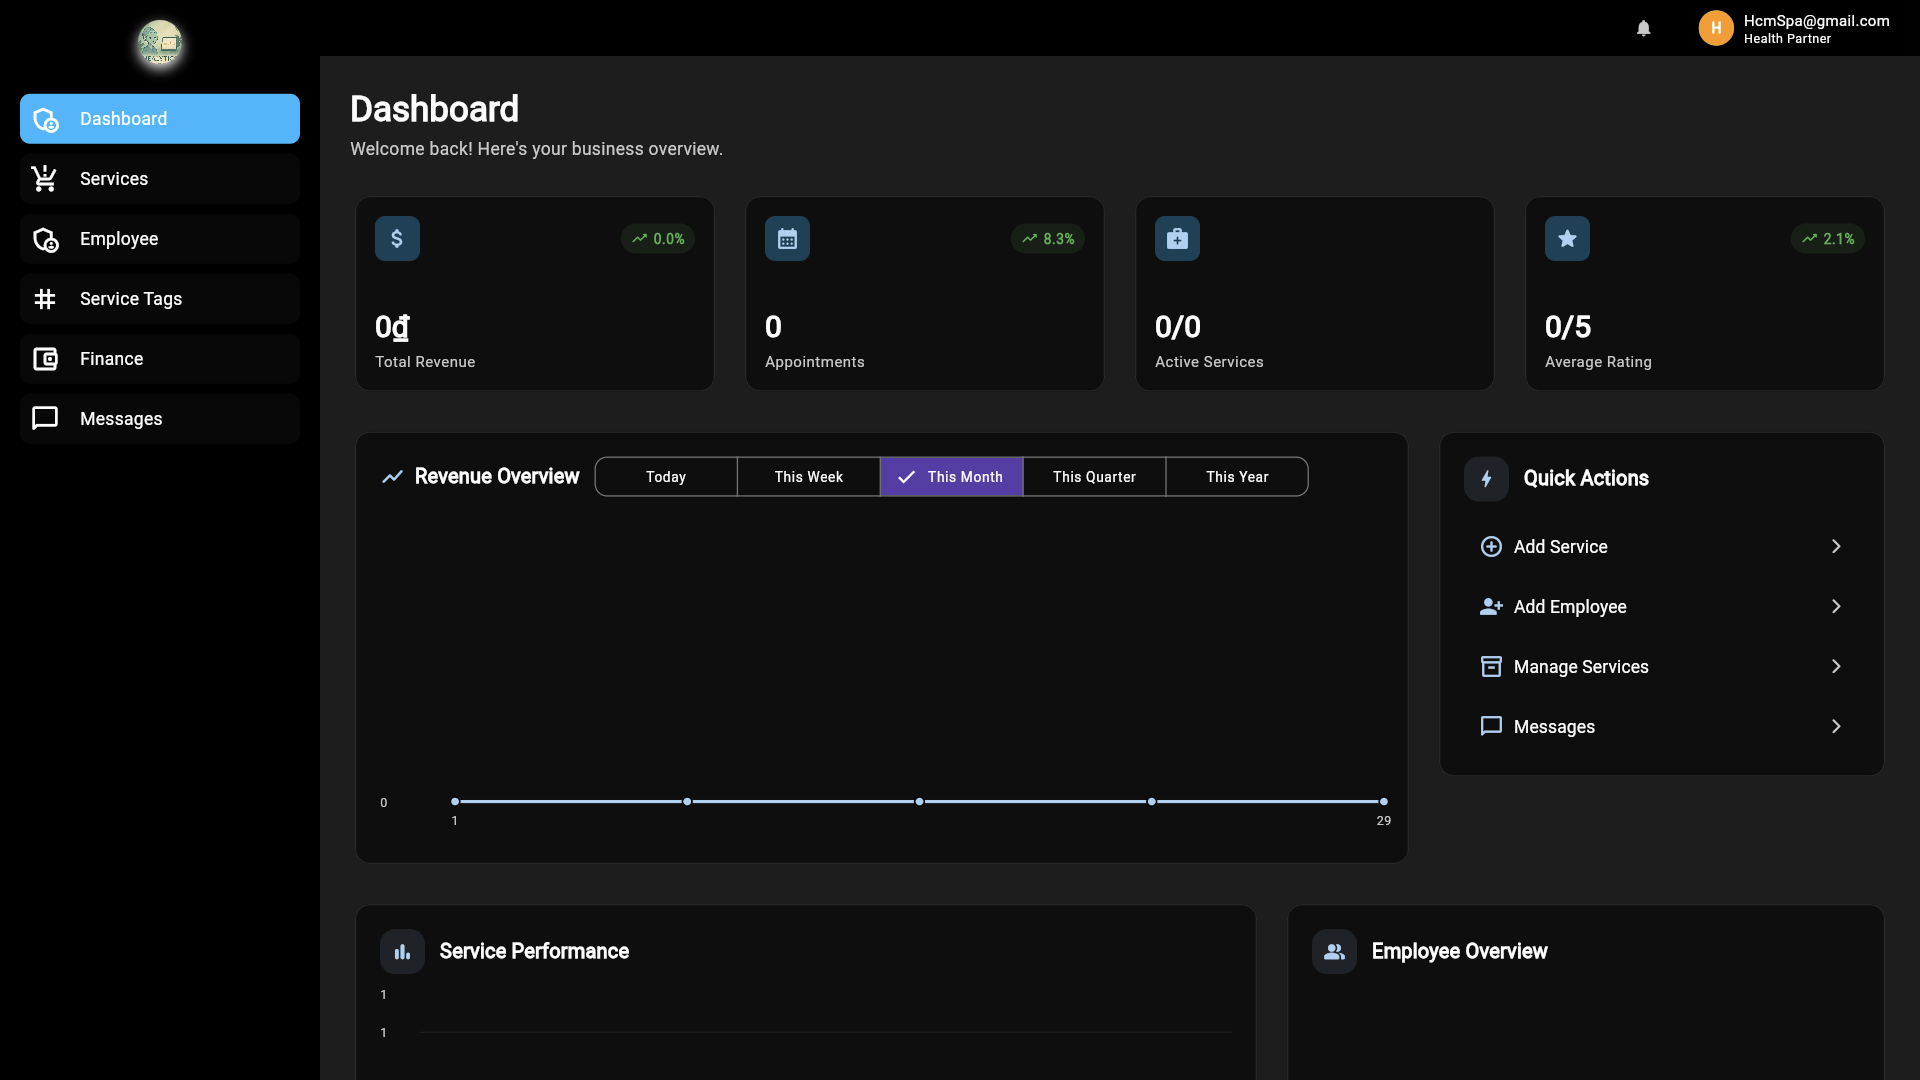
\includegraphics[width=0.85\textwidth]{Images/Hiện thực/partner/fig_partner_dashboard.png}
    \vspace{1em}
    \caption{Dashboard Đối tác -- tổng quan kinh doanh}
    \label{fig:partner_dashboard}
\end{figure}

\begin{itemize}
    \item \textbf{KPI tổng hợp:} Bao gồm (1)~Doanh thu tổng, (2)~Số lịch hẹn, (3)~Dịch vụ đang hoạt động, và (4)~Đánh giá trung bình.
    \item \textbf{Biểu đồ phân tích:} Cung cấp biểu đồ trực quan hóa xu hướng doanh thu theo thời gian.
    \item \textbf{Quick Actions (Thao tác nhanh):} Cho phép truy cập nhanh để thêm dịch vụ, quản lý nhân viên, hoặc kiểm tra tin nhắn khách hàng.
\end{itemize}


% ===========================================================================
% 6.3.4  PHÂN HỆ TRANG QUẢN TRỊ (ADMIN PORTAL)
% ===========================================================================
\subsection{Hiện thực Phân hệ Trang Quản trị (Admin Portal)}

Phân hệ Quản trị cung cấp cho quản trị viên công cụ giám sát và kiểm duyệt toàn bộ hệ thống. Admin đăng nhập qua trang đăng nhập chuyên biệt và truy cập vào hệ thống quản trị với 5 module chính: Dashboard, Finance, Category, Provider, và Notifications.

\begin{figure}[H]
    \centering
    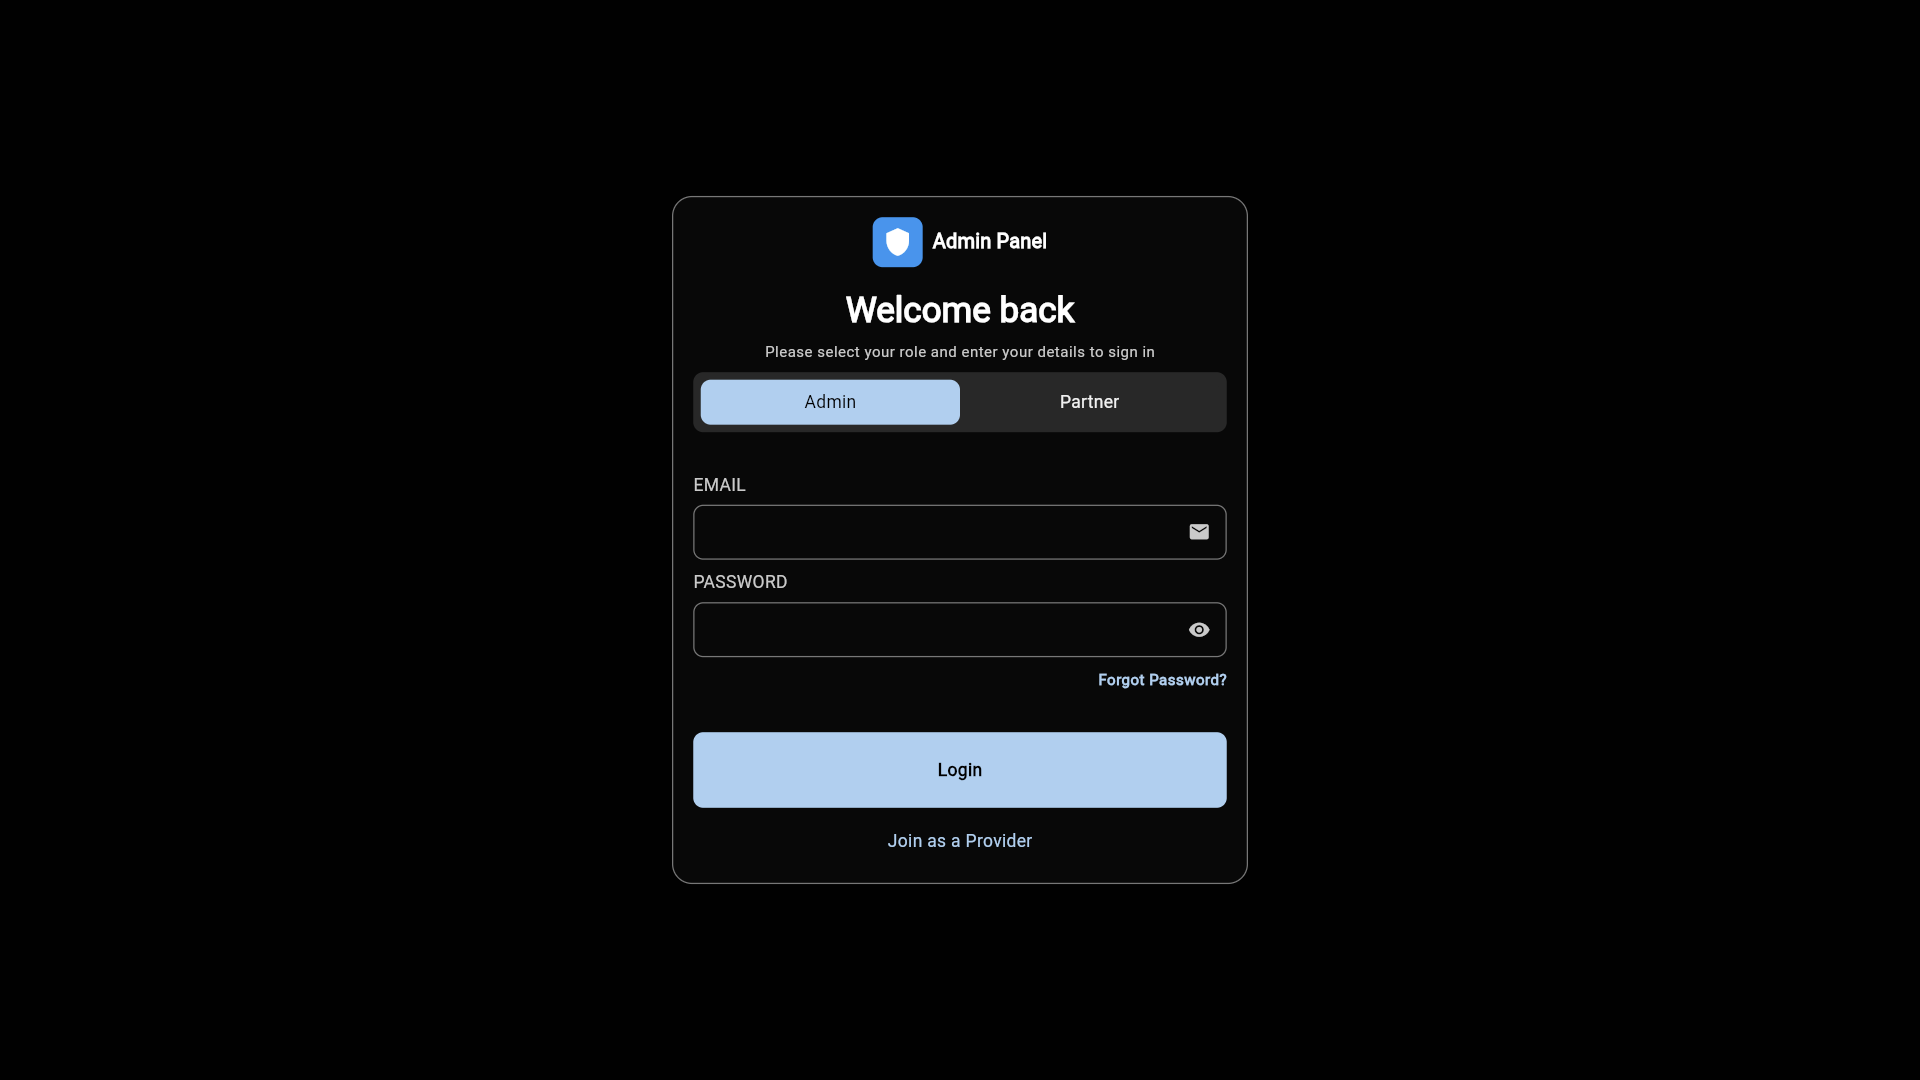
\includegraphics[width=0.6\textwidth]{Images/Hiện thực/admin/fig_admin_login.png}
    \vspace{1em}
    \caption{Màn hình đăng nhập Admin Portal}
    \label{fig:admin_login}
\end{figure}

\begin{itemize}
    \item \textbf{Thao tác xác thực:} Quản trị viên nhập tài khoản quản trị để truy cập hệ thống.
    \item \textbf{Thao tác điều hướng sau đăng nhập:} Hệ thống chuyển thẳng tới Dashboard tổng quan.
\end{itemize}

\begin{enumerate}
    \item \textbf{KPI Cards (hàng trên):} Doanh thu tổng (Gross Revenue), số giao dịch thành công, tổng số đối tác, tỷ lệ booking thành công, tỷ lệ thất bại, tỷ lệ hủy, giá trị booking trung bình, và số lượng thông báo vận hành.

    \item \textbf{Finance Trend (giữa):} Biểu đồ xu hướng doanh thu theo ngày (gross revenue, net revenue, refund pressure) kèm Finance Summary tổng hợp các chỉ số tài chính cốt lõi.

    \item \textbf{Booking Outcomes \& Transaction Health (dưới):} Phân tích chi tiết kết quả booking (Successful/Failed/Canceled) và sức khỏe giao dịch (Paid/Pending/Refunded/Failed/Canceled).

    \item \textbf{Top Revenue Partners \& Services:} Xếp hạng 5 đối tác và 5 dịch vụ có doanh thu cao nhất, kèm số booking và tỷ lệ thành công.
\end{enumerate}

\begin{figure}[H]
    \centering
    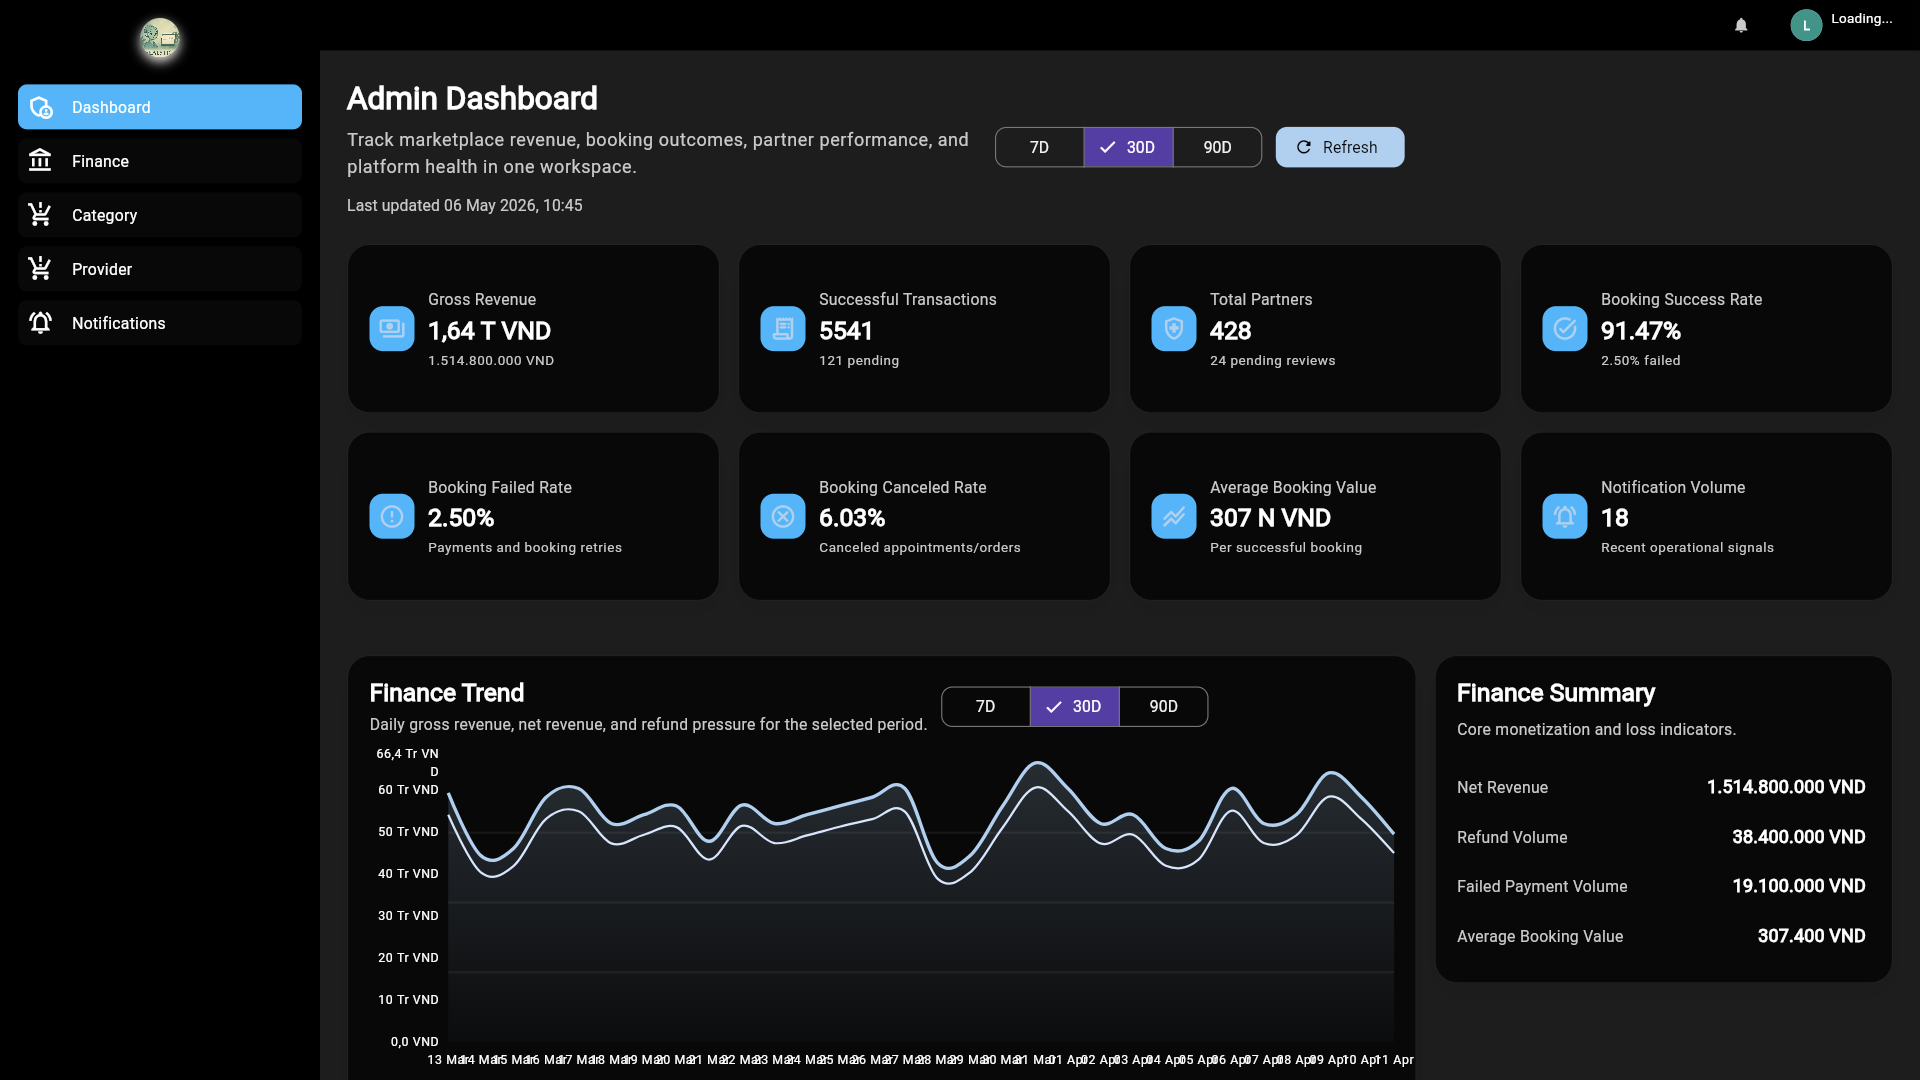
\includegraphics[width=0.92\textwidth]{Images/Hiện thực/admin/fig_admin_dashboard_top.png}
    \vspace{1em}
    \caption{Admin Dashboard -- phần trên: KPI Cards và Finance Trend}
    \label{fig:admin_dashboard_top}
\end{figure}

Hình~\ref{fig:admin_dashboard_top} hiển thị phần trên của Dashboard quản trị:
\begin{itemize}
    \item \textbf{Hàng KPI Cards:} Trình bày 8 chỉ số cốt lõi bao gồm Gross Revenue (Doanh thu tổng), Successful Transactions (Giao dịch thành công), Total Partners (Tổng đối tác, kèm số lượng chờ duyệt), tỷ lệ Booking (Thành công/Thất bại/Hủy), Average Booking Value (Giá trị trung bình), và Notification Volume.
    \item \textbf{Finance Trend:} Biểu đồ minh họa doanh thu trong 30 ngày qua, đi kèm với bảng tóm tắt tài chính (Finance Summary) chi tiết.
\end{itemize}

\begin{figure}[H]
    \centering
    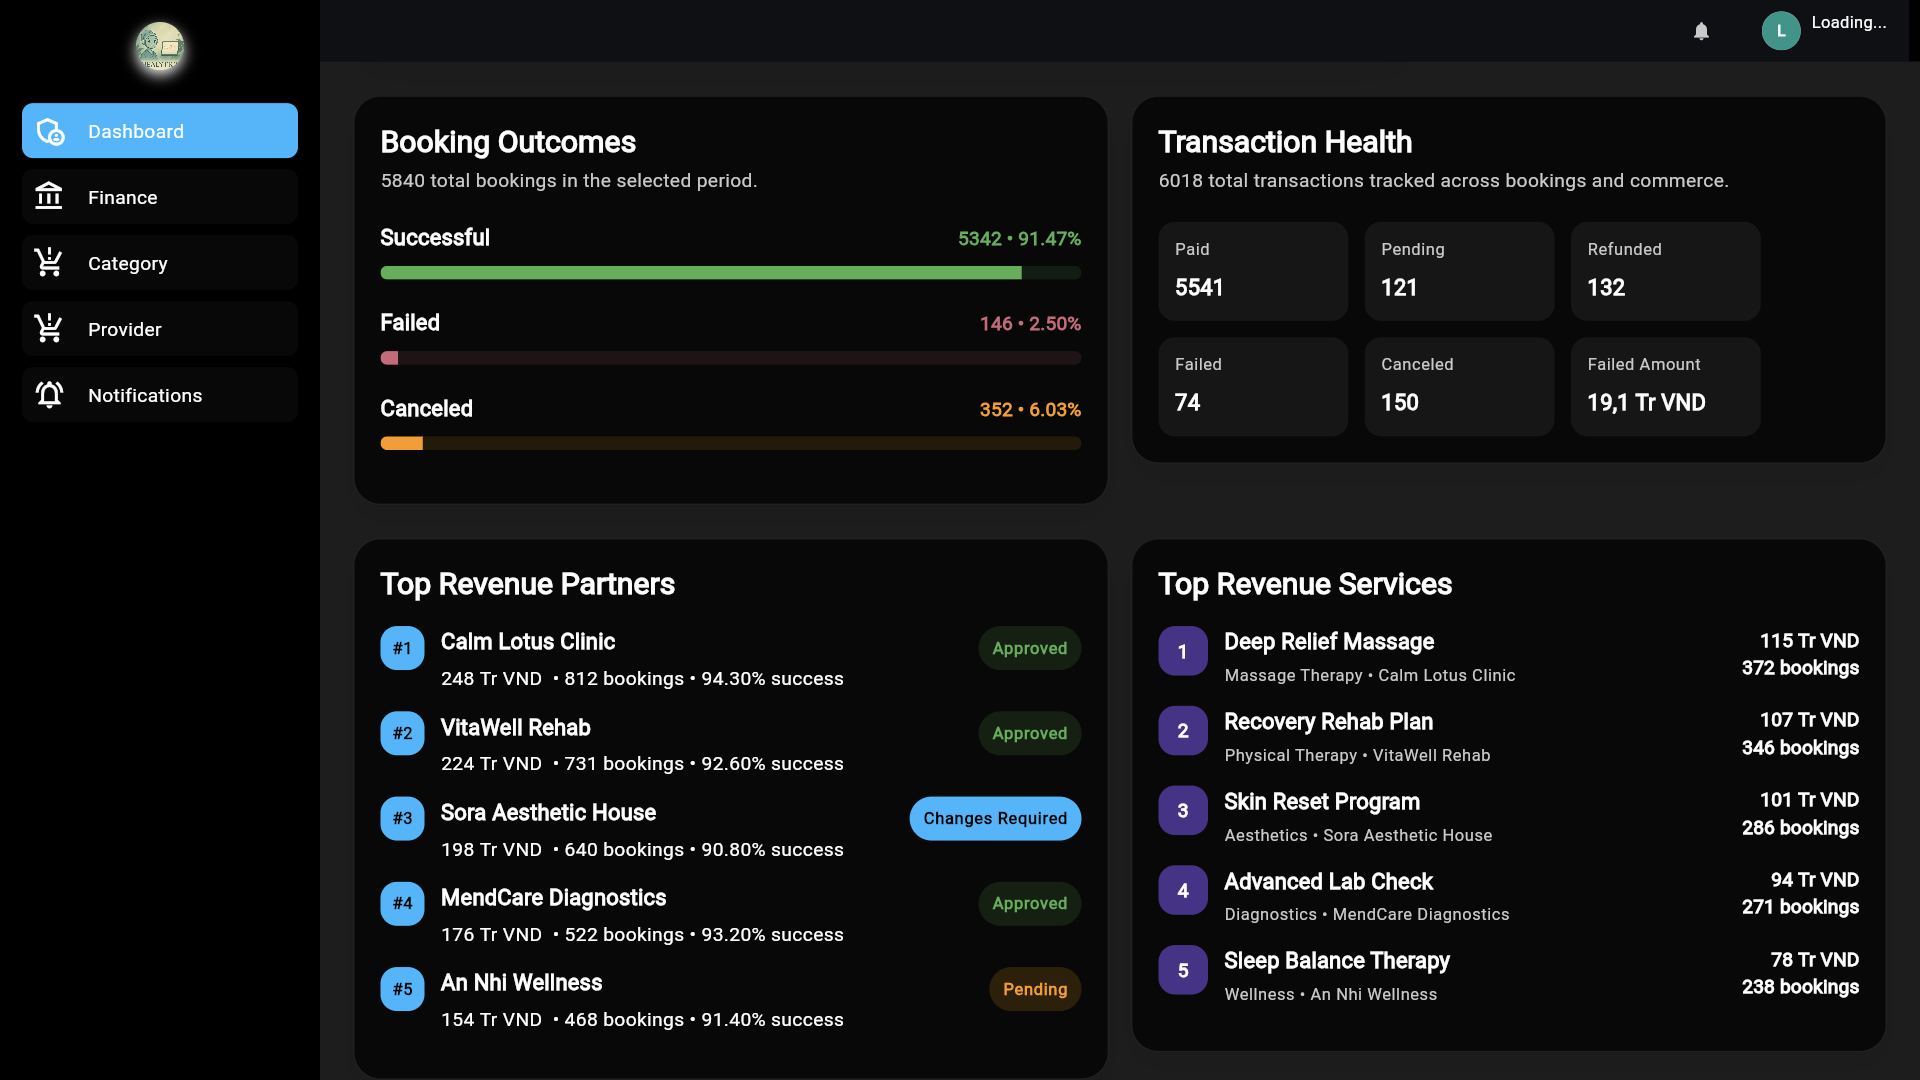
\includegraphics[width=0.92\textwidth]{Images/Hiện thực/admin/fig_admin_dashboard_bottom.png}
    \vspace{1em}
    \caption{Admin Dashboard -- phần dưới: Booking Outcomes và Top Revenue}
    \label{fig:admin_dashboard_bottom}
\end{figure}

Hình~\ref{fig:admin_dashboard_bottom} hiển thị phần dưới của Dashboard quản trị:
\begin{itemize}
    \item \textbf{Booking Outcomes:} Phân tích chi tiết trạng thái của các lượt đặt lịch (Successful, Failed, Canceled).
    \item \textbf{Transaction Health:} Thống kê tình trạng sức khỏe của các giao dịch trên hệ thống.
    \item \textbf{Bảng xếp hạng (Leaderboards):} Liệt kê Top Revenue Partners (5 đối tác có doanh thu cao nhất) và Top Revenue Services (5 dịch vụ bán chạy nhất).
\end{itemize}

\begin{figure}[H]
    \centering
    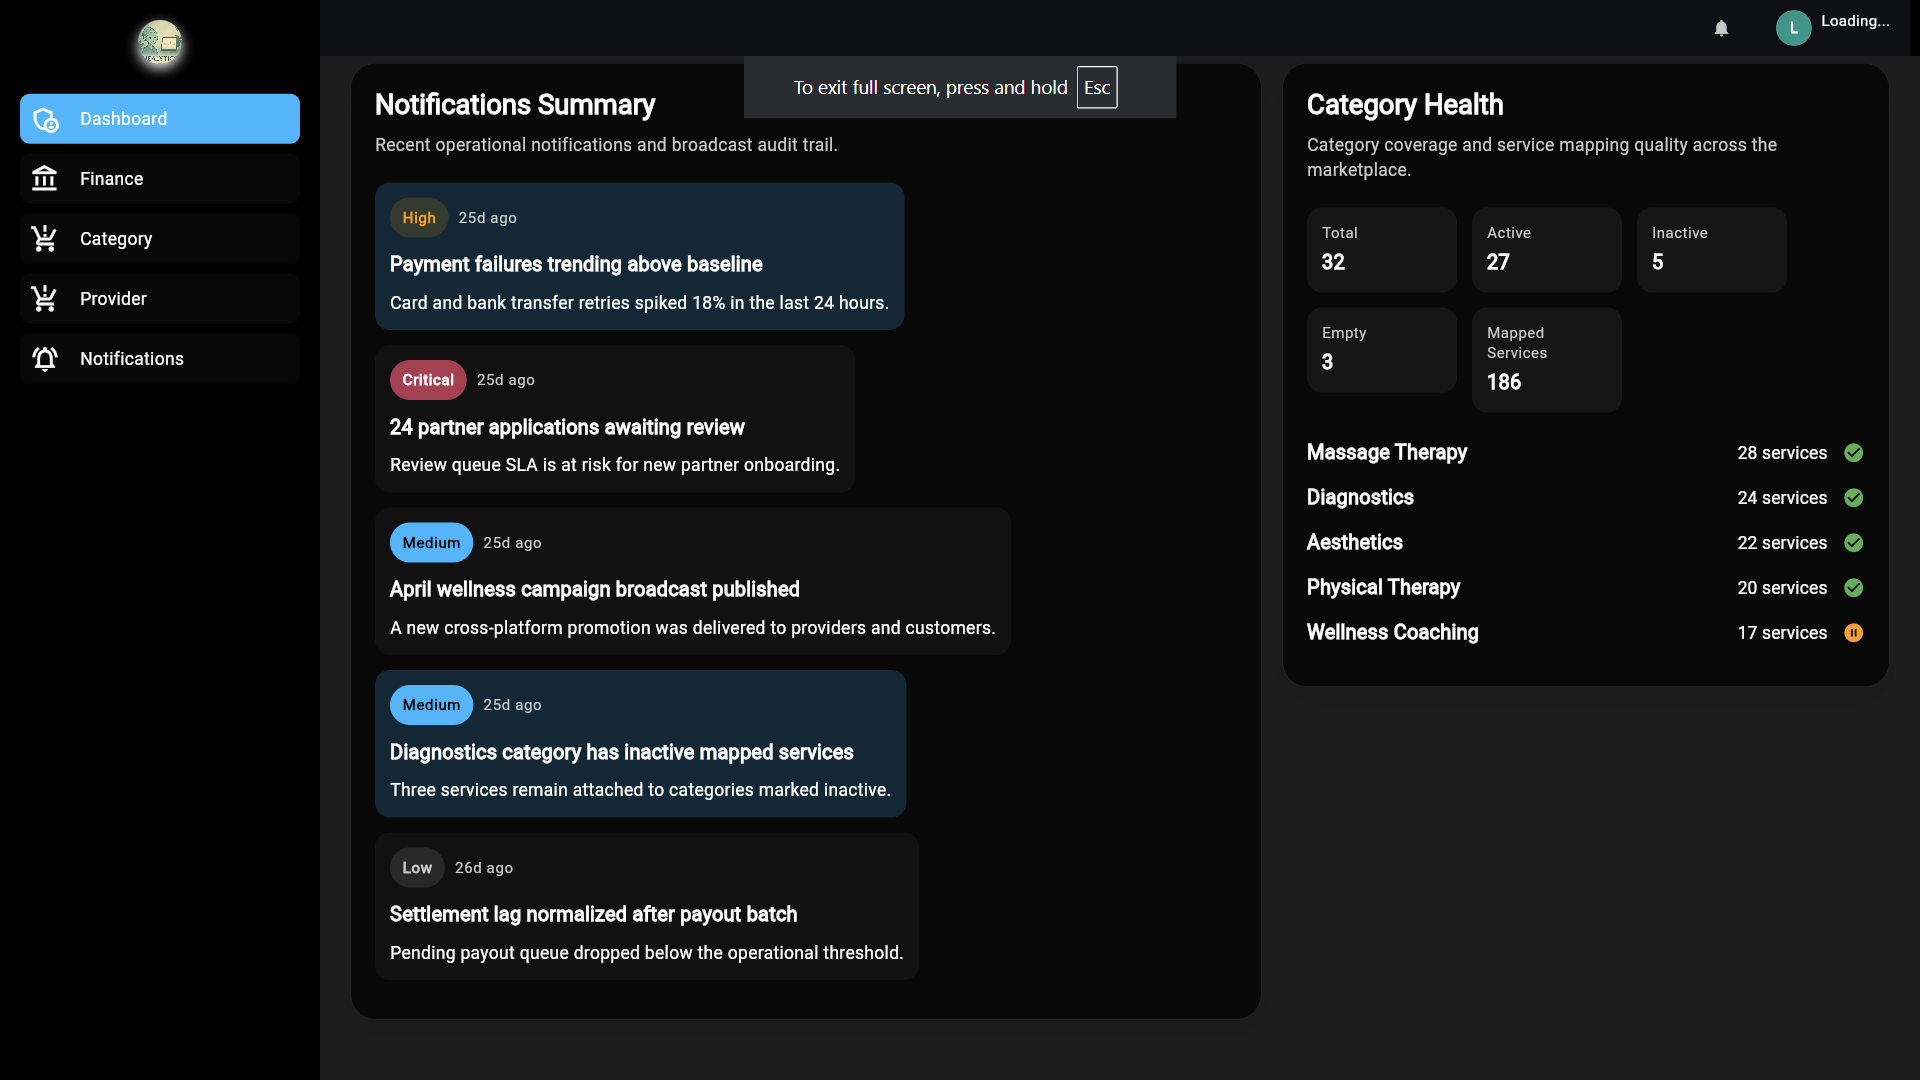
\includegraphics[width=0.92\textwidth]{Images/Hiện thực/admin/fig_admin_dashboard_notifications.png}
    \vspace{1em}
    \caption{Admin Dashboard -- khối cảnh báo và thông báo vận hành}
    \label{fig:admin_dashboard_notifications}
\end{figure}

\begin{itemize}
    \item \textbf{Thao tác giám sát:} Quản trị viên theo dõi cảnh báo quan trọng và sự kiện vận hành theo thời gian thực.
    \item \textbf{Thao tác xử lý nhanh:} Truy cập nhanh vào module liên quan để xử lý giao dịch lỗi hoặc thông báo khẩn.
\end{itemize}

Tab Overview hiển thị 8 KPI tài chính chính: Gross Volume, Net Revenue, Platform Fees, Refund Exposure, Failed Payments, Pending Payouts, Held Payouts, và Unreconciled --- mỗi chỉ số kèm tỷ lệ thay đổi so với kỳ trước. Bên dưới là bảng Revenue Trend theo ngày (Gross/Net/Refunds/Payouts) và hệ thống bộ lọc đa chiều.

\begin{figure}[H]
    \centering
    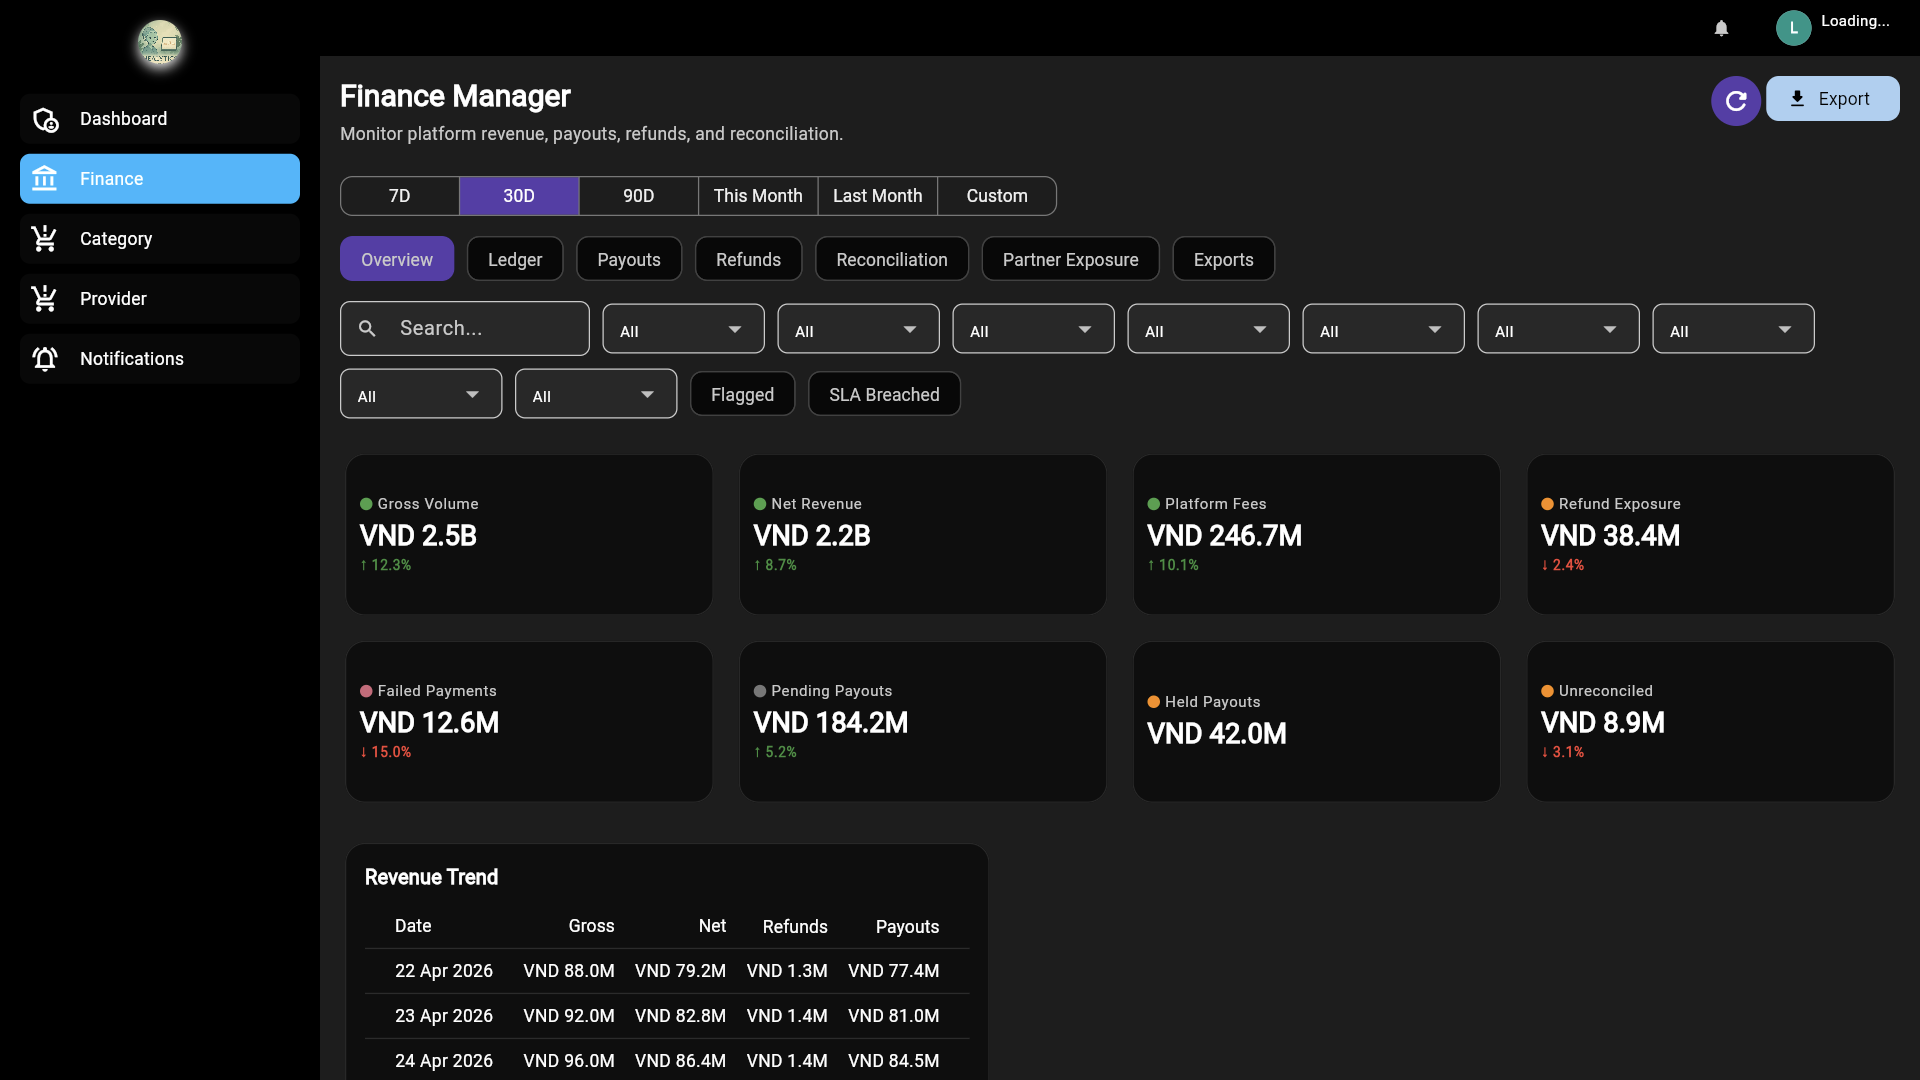
\includegraphics[width=0.85\textwidth]{Images/Hiện thực/admin/fig_admin_finance_overview.png}
    \vspace{1em}
    \caption{Finance Manager -- Tab Overview}
    \label{fig:admin_finance}
\end{figure}

\begin{figure}[H]
    \centering
    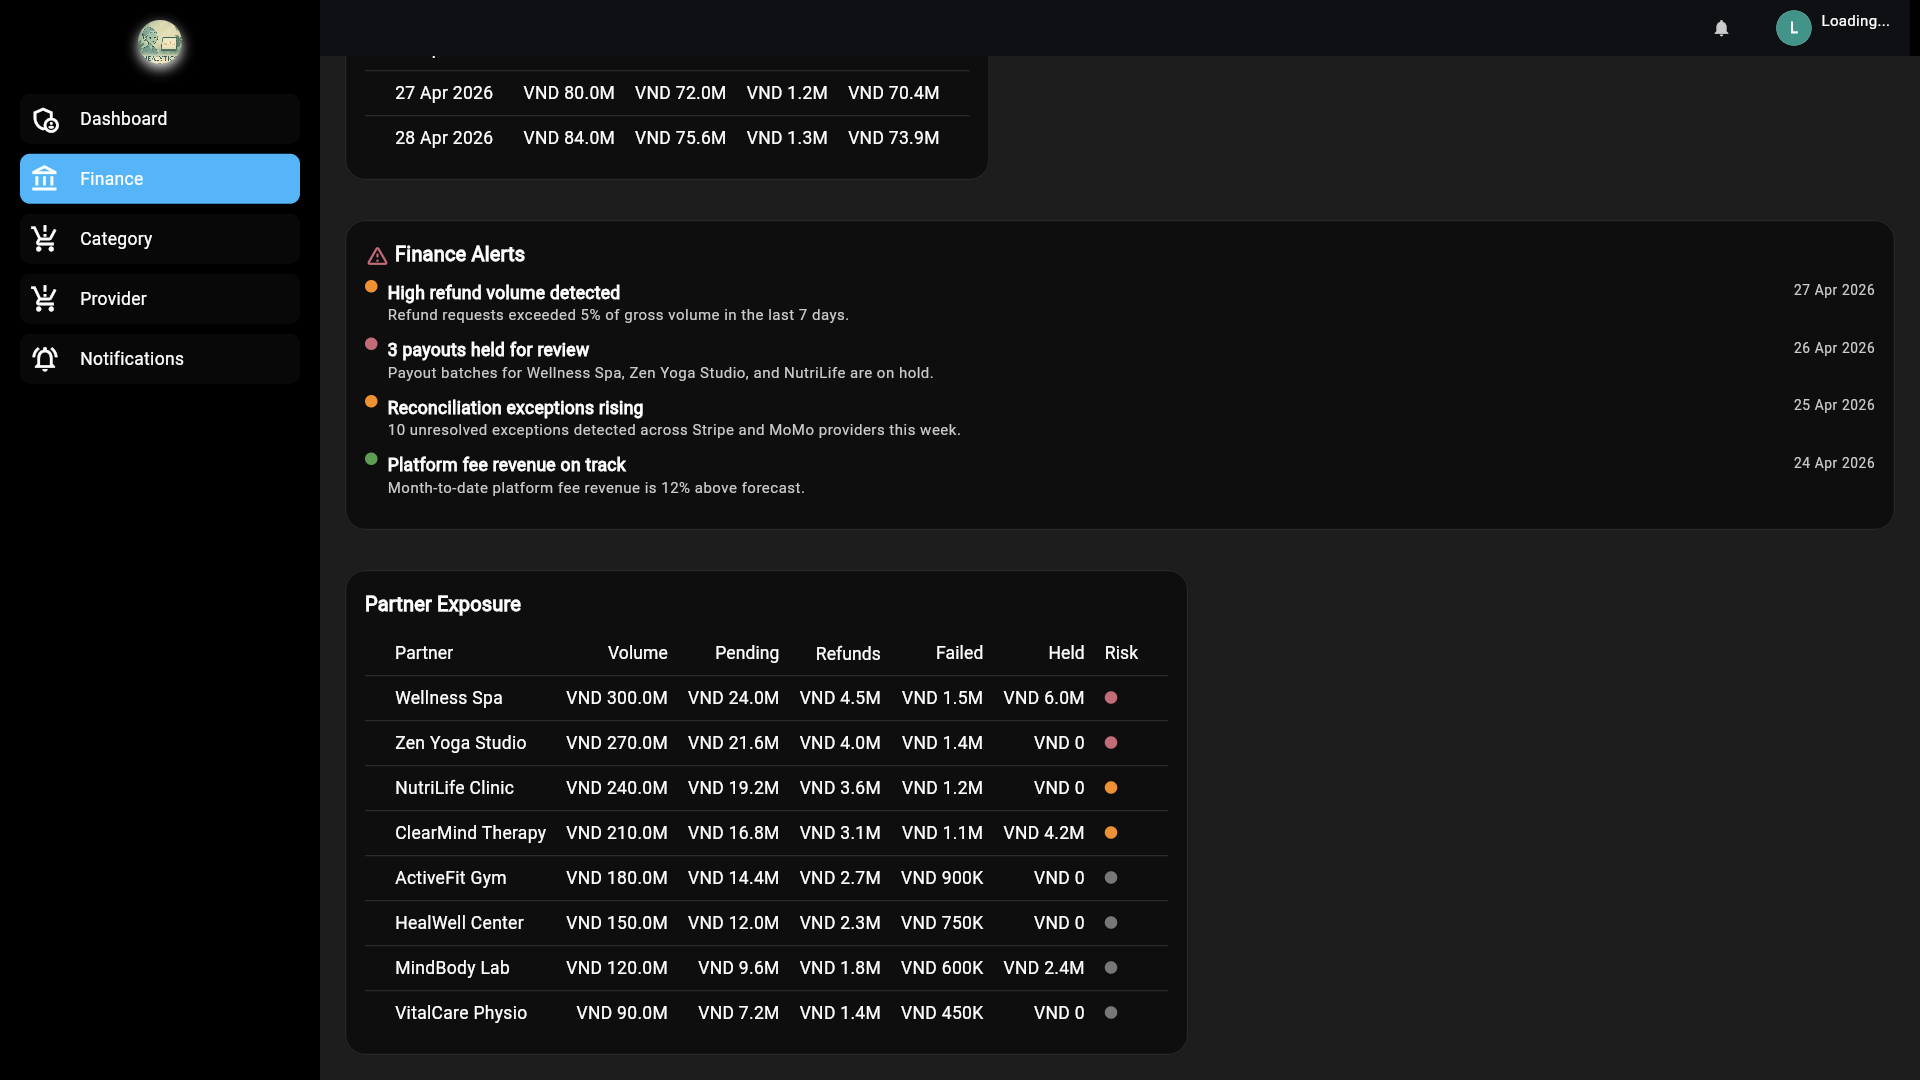
\includegraphics[width=0.85\textwidth]{Images/Hiện thực/admin/fig_admin_finance_revenue.png}
    \vspace{1em}
    \caption{Finance Manager -- Tab Revenue Trend chi tiết}
    \label{fig:admin_finance_revenue}
\end{figure}

Hình~\ref{fig:admin_finance} hiển thị tab Overview của module quản lý tài chính:
\begin{itemize}
    \item \textbf{KPI tài chính (8 chỉ số):} Bao gồm Gross Volume, Net Revenue, Platform Fees, Refund Exposure, Failed Payments, Pending Payouts, Held Payouts, và Unreconciled. Mỗi chỉ số đều kèm theo tỷ lệ thay đổi so với kỳ báo cáo trước.
    \item \textbf{Bảng Revenue Trend:} Thống kê và hiển thị chi tiết dòng tiền theo từng ngày (Gross, Net, Refunds, Payouts).
\end{itemize}

\subsubsection{Quy trình Kiểm duyệt Đối tác}

Đây là quy trình nghiệp vụ quan trọng nhất của Admin Portal. Quản trị viên thực hiện các bước sau:

\paragraph{Bước 1 -- Xem danh sách đối tác chờ duyệt}

Tại menu ``Provider'', quản trị viên thấy danh sách toàn bộ đối tác với thông tin: tên, ID, loại hình kinh doanh, ngày nộp, trạng thái (Pending/Active/Rejected), và các nút hành động. Cột ``Actions'' hiển thị nút ``Review Application'' cho các hồ sơ đang chờ duyệt (Hình~\ref{fig:admin_provider_list}).

\begin{figure}[H]
    \centering
    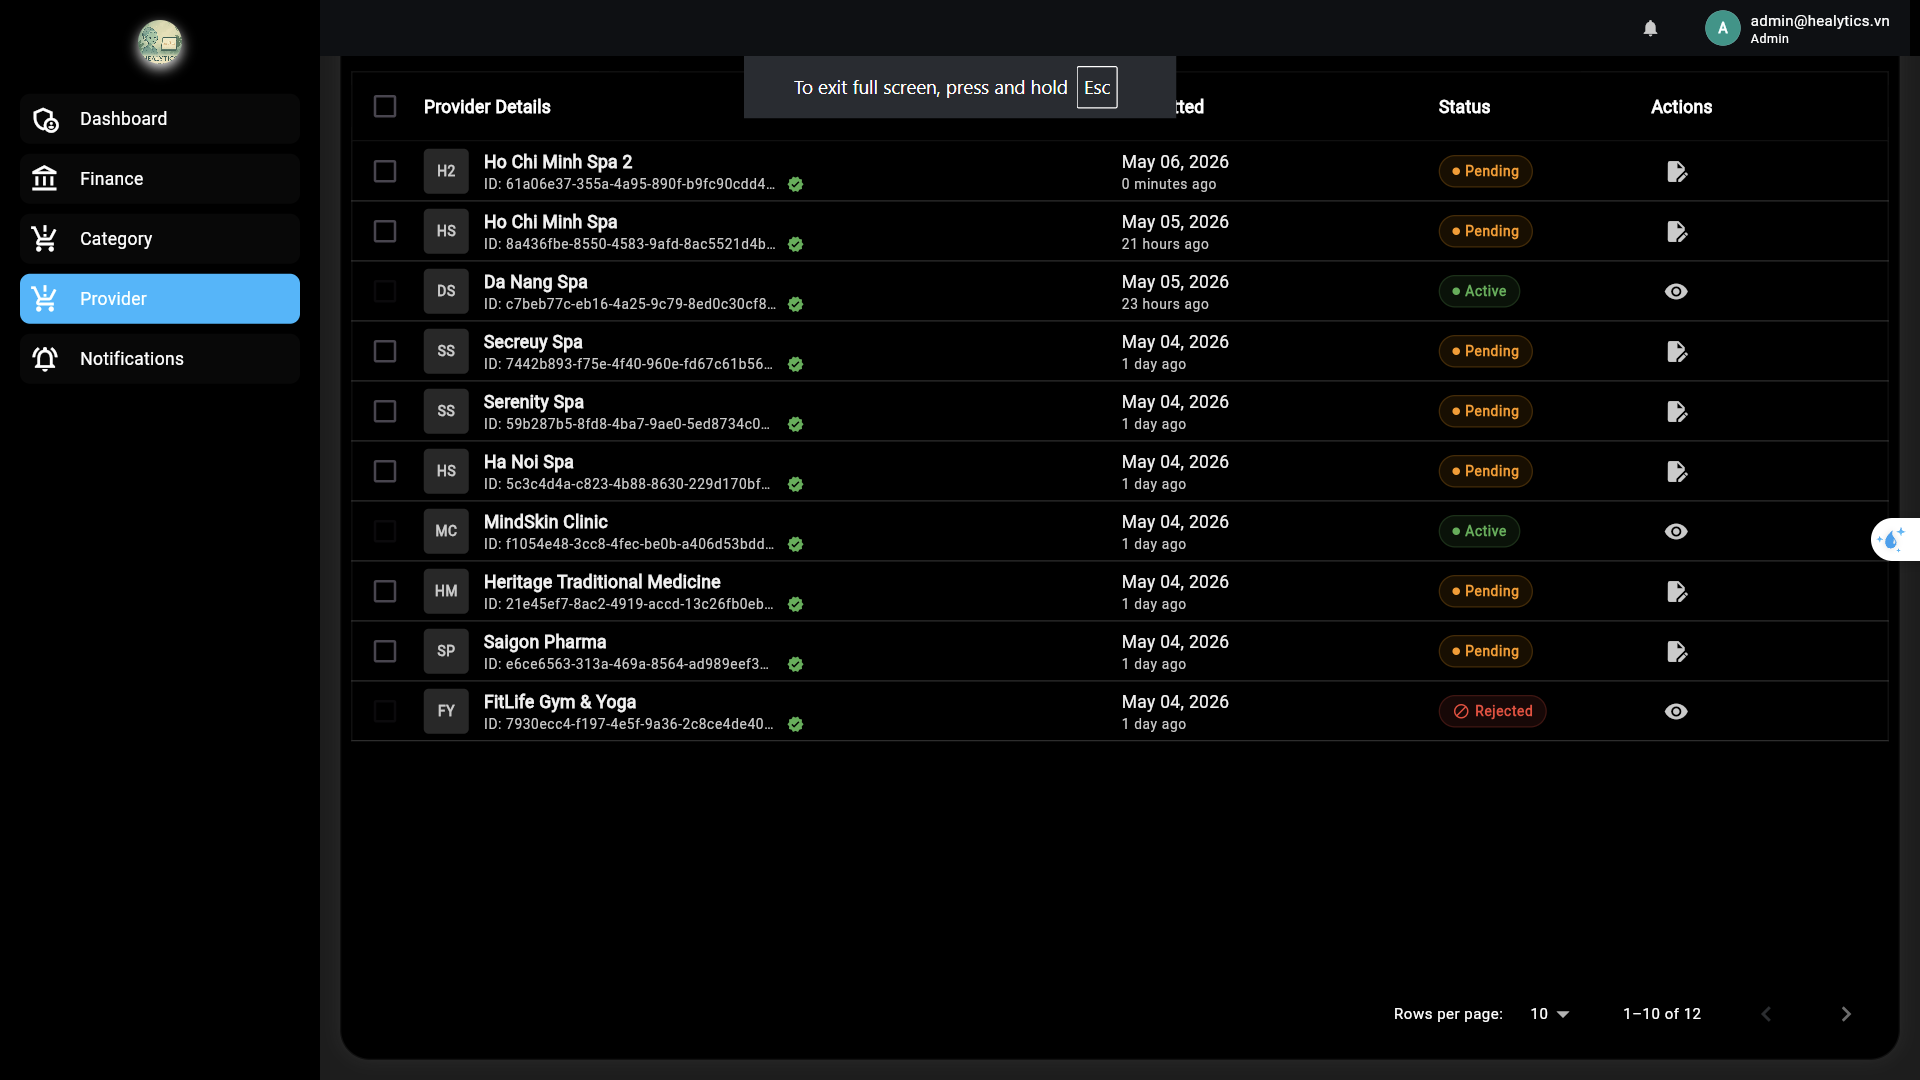
\includegraphics[width=0.85\textwidth]{Images/Hiện thực/admin/fig_admin_provider_list_new.png}
    \vspace{1em}
    \caption{Danh sách đối tác chờ duyệt tại module Provider}
    \label{fig:admin_provider_list}
\end{figure}

Hình~\ref{fig:admin_provider_list} hiển thị danh sách toàn bộ đối tác:
\begin{itemize}
    \item \textbf{Thông tin hiển thị:} Tên đối tác, ID, loại hình kinh doanh, ngày nộp hồ sơ, và trạng thái hiện tại (Pending/Active/Rejected).
    \item \textbf{Cột Actions (Hành động):} Cung cấp nút ``Review Application'' (hiển thị màu xanh khi hover) cho phép quản trị viên truy cập nhanh vào các hồ sơ đang trong trạng thái chờ duyệt.
\end{itemize}

\paragraph{Bước 2 -- Xem chi tiết và xét duyệt từng trường}

Khi nhấn ``Review Application'', quản trị viên được chuyển đến trang chi tiết hồ sơ (Hình~\ref{fig:admin_detail_top} và Hình~\ref{fig:admin_detail_bottom}) gồm:

\begin{itemize}
    \item \textbf{Business Overview:} Tên thương hiệu, mã số thuế, loại hình, địa chỉ (hiển thị trên bản đồ), và đường dẫn.
    \item \textbf{Account \& Contact:} Email và số điện thoại liên hệ.
    \item \textbf{Legal Representative:} Họ tên, chức vụ, loại giấy tờ, số giấy tờ, ngày cấp.
    \item \textbf{KYC Documents (cột phải):} Ảnh CCCD mặt trước/sau (có nút zoom), Giấy phép kinh doanh (có nút tải xuống).
\end{itemize}

Mỗi trường có biểu tượng \checkmark{} (hợp lệ) và \textit{bút chỉnh sửa} (cần sửa). Khi admin đánh dấu một trường cần sửa, hệ thống hiển thị popup ``Revision Note'' để nhập lý do cụ thể (Hình~\ref{fig:admin_revision_note}). Cuối trang, admin chọn \textbf{``Approve Provider''} (nút xanh) hoặc \textbf{``Reject Application''} (nút đỏ).

\begin{figure}[H]
    \centering
    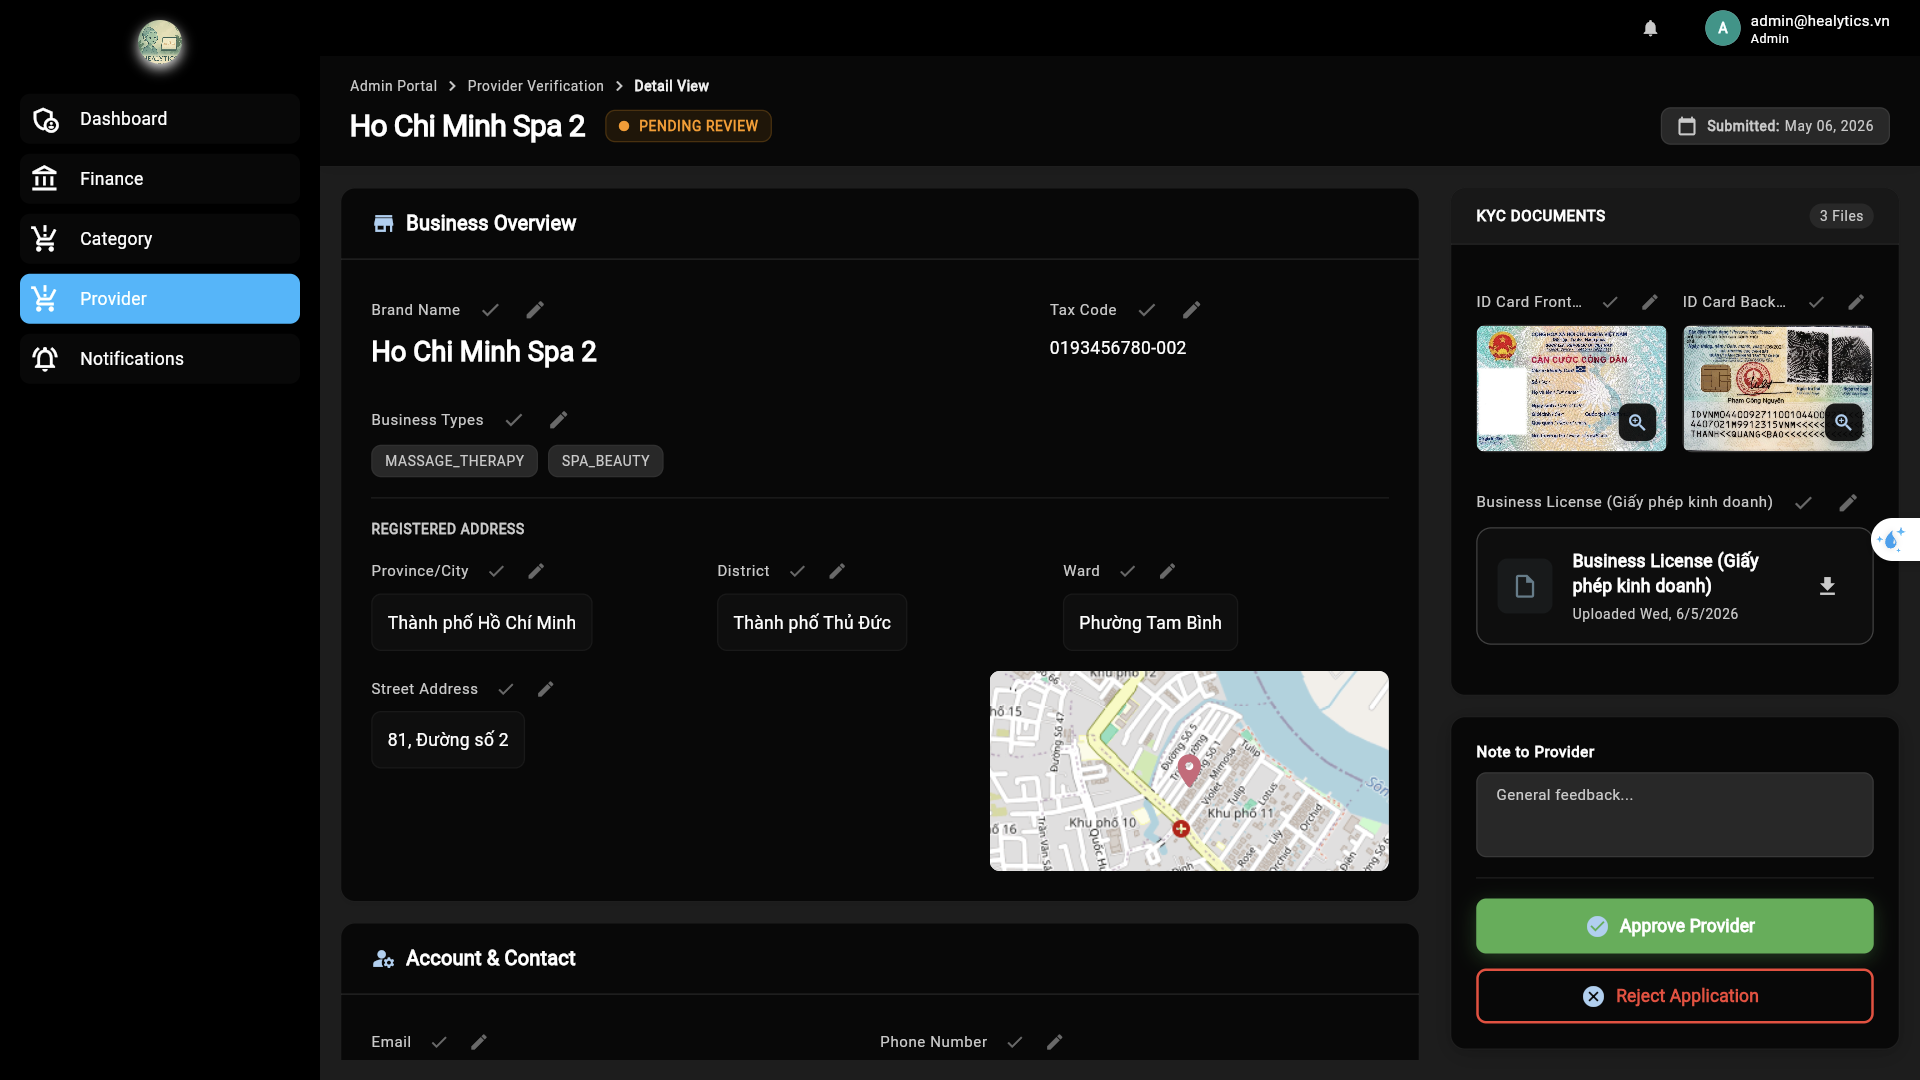
\includegraphics[width=0.92\textwidth]{Images/Hiện thực/admin/fig_admin_provider_detail_top.png}
    \vspace{1em}
    \caption{Trang xét duyệt đối tác -- phần trên: Business Overview và KYC Documents}
    \label{fig:admin_detail_top}
\end{figure}

Hình~\ref{fig:admin_detail_top} hiển thị phần trên của trang chi tiết xét duyệt hồ sơ:
\begin{itemize}
    \item \textbf{Ngữ cảnh \& Trạng thái:} Sử dụng breadcrumb ``Provider Verification > Detail View'' và tiêu đề kèm badge \textbf{PENDING REVIEW} cùng ngày nộp hồ sơ.
    \item \textbf{Business Overview:} Liệt kê Brand Name, Tax Code, Business Types, và Registered Address (được trực quan hóa trên bản đồ Google Maps).
    \item \textbf{KYC Documents (cột phải):} Hiển thị ảnh CCCD mặt trước/sau (có tính năng phóng to) và Giấy phép kinh doanh (có tính năng tải xuống).
    \item \textbf{Công cụ đánh giá:} Mỗi trường thông tin đều kèm biểu tượng \checkmark{} (đánh dấu hợp lệ) và biểu tượng bút chỉnh sửa (đánh dấu có lỗi).
\end{itemize}

\begin{figure}[H]
    \centering
    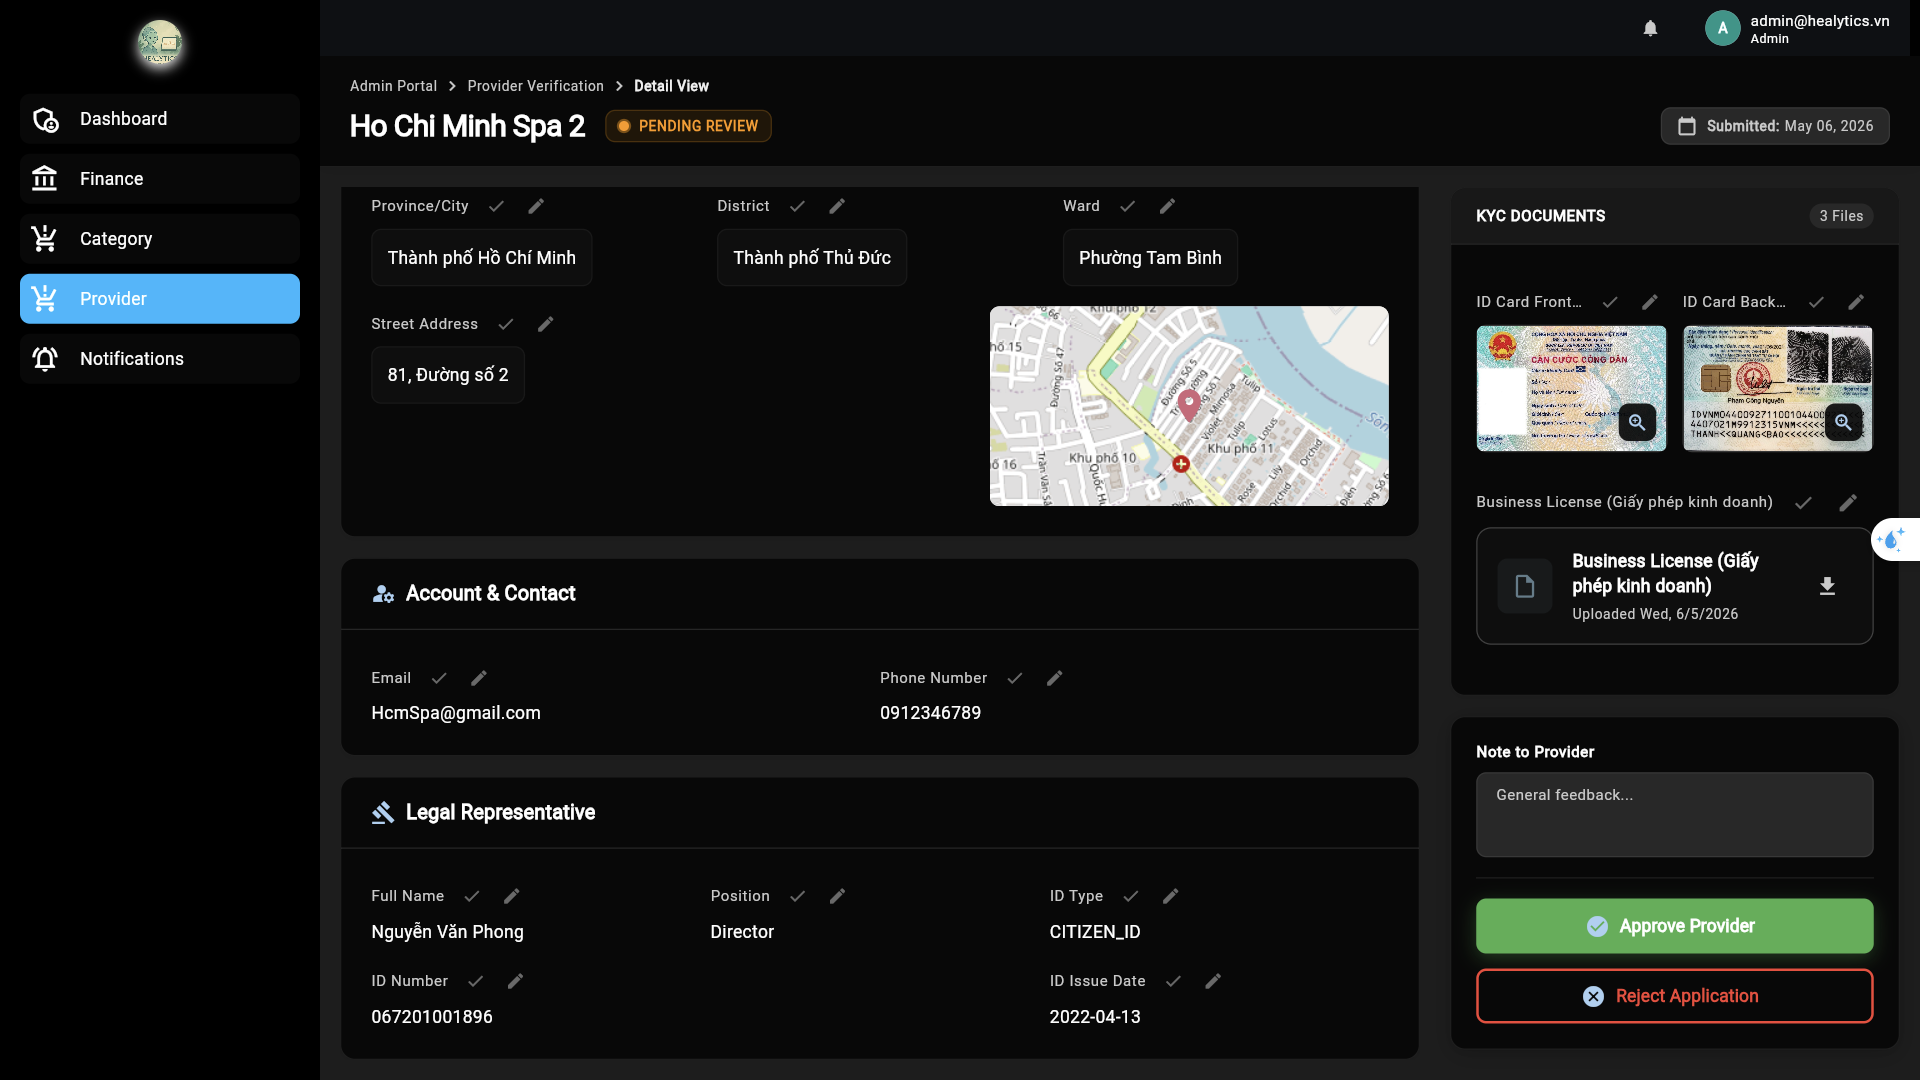
\includegraphics[width=0.92\textwidth]{Images/Hiện thực/admin/fig_admin_provider_detail_bottom.png}
    \vspace{1em}
    \caption{Trang xét duyệt đối tác -- phần dưới: Contact, Legal Representative và nút hành động}
    \label{fig:admin_detail_bottom}
\end{figure}

Hình~\ref{fig:admin_detail_bottom} hiển thị phần dưới của trang chi tiết xét duyệt hồ sơ:
\begin{itemize}
    \item \textbf{Thông tin chi tiết:} Bao gồm phần \textbf{Account \& Contact} (Email, Phone) và phần \textbf{Legal Representative} (Full Name, Position, ID Type, ID Number, ID Issue Date).
    \item \textbf{Hành động xét duyệt:} Cung cấp hai nút quyết định chính là \textbf{``Approve Provider''} (chấp thuận - nút xanh) và \textbf{``Reject Application''} (từ chối - nút đỏ).
    \item \textbf{Phản hồi chung:} Ô \textbf{Note to Provider} cho phép quản trị viên nhập nhận xét và hướng dẫn tổng thể cho đối tác.
\end{itemize}

% Hình bản đồ Business Overview -- tạm comment vì nội dung trùng với Hình admin_detail_top
% \begin{figure}[H]
%     \centering
%     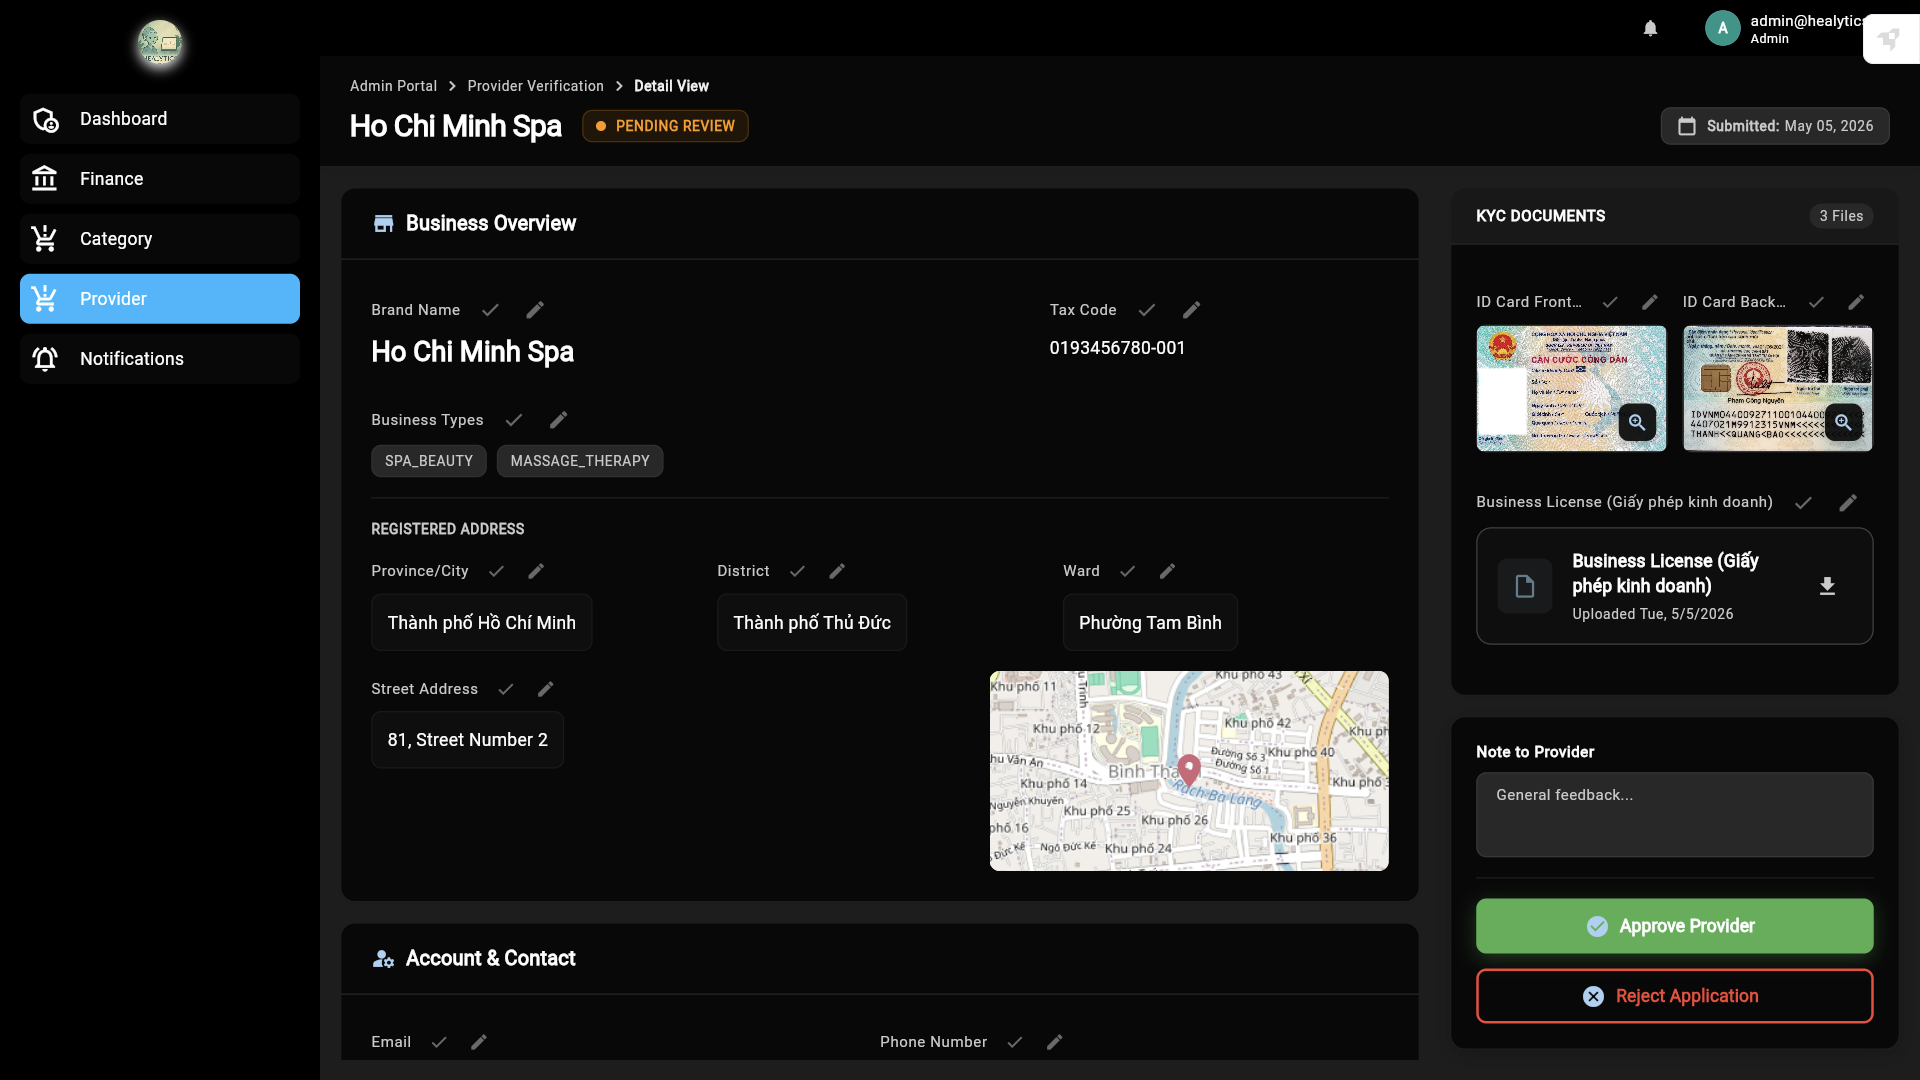
\includegraphics[width=0.92\textwidth]{Images/Hiện thực/admin/fig_admin_verify_business_top.png}
%     \caption{Business Overview -- bản đồ vị trí kinh doanh}
%     \label{fig:admin_verify_map}
% \end{figure}

\begin{figure}[H]
    \centering
    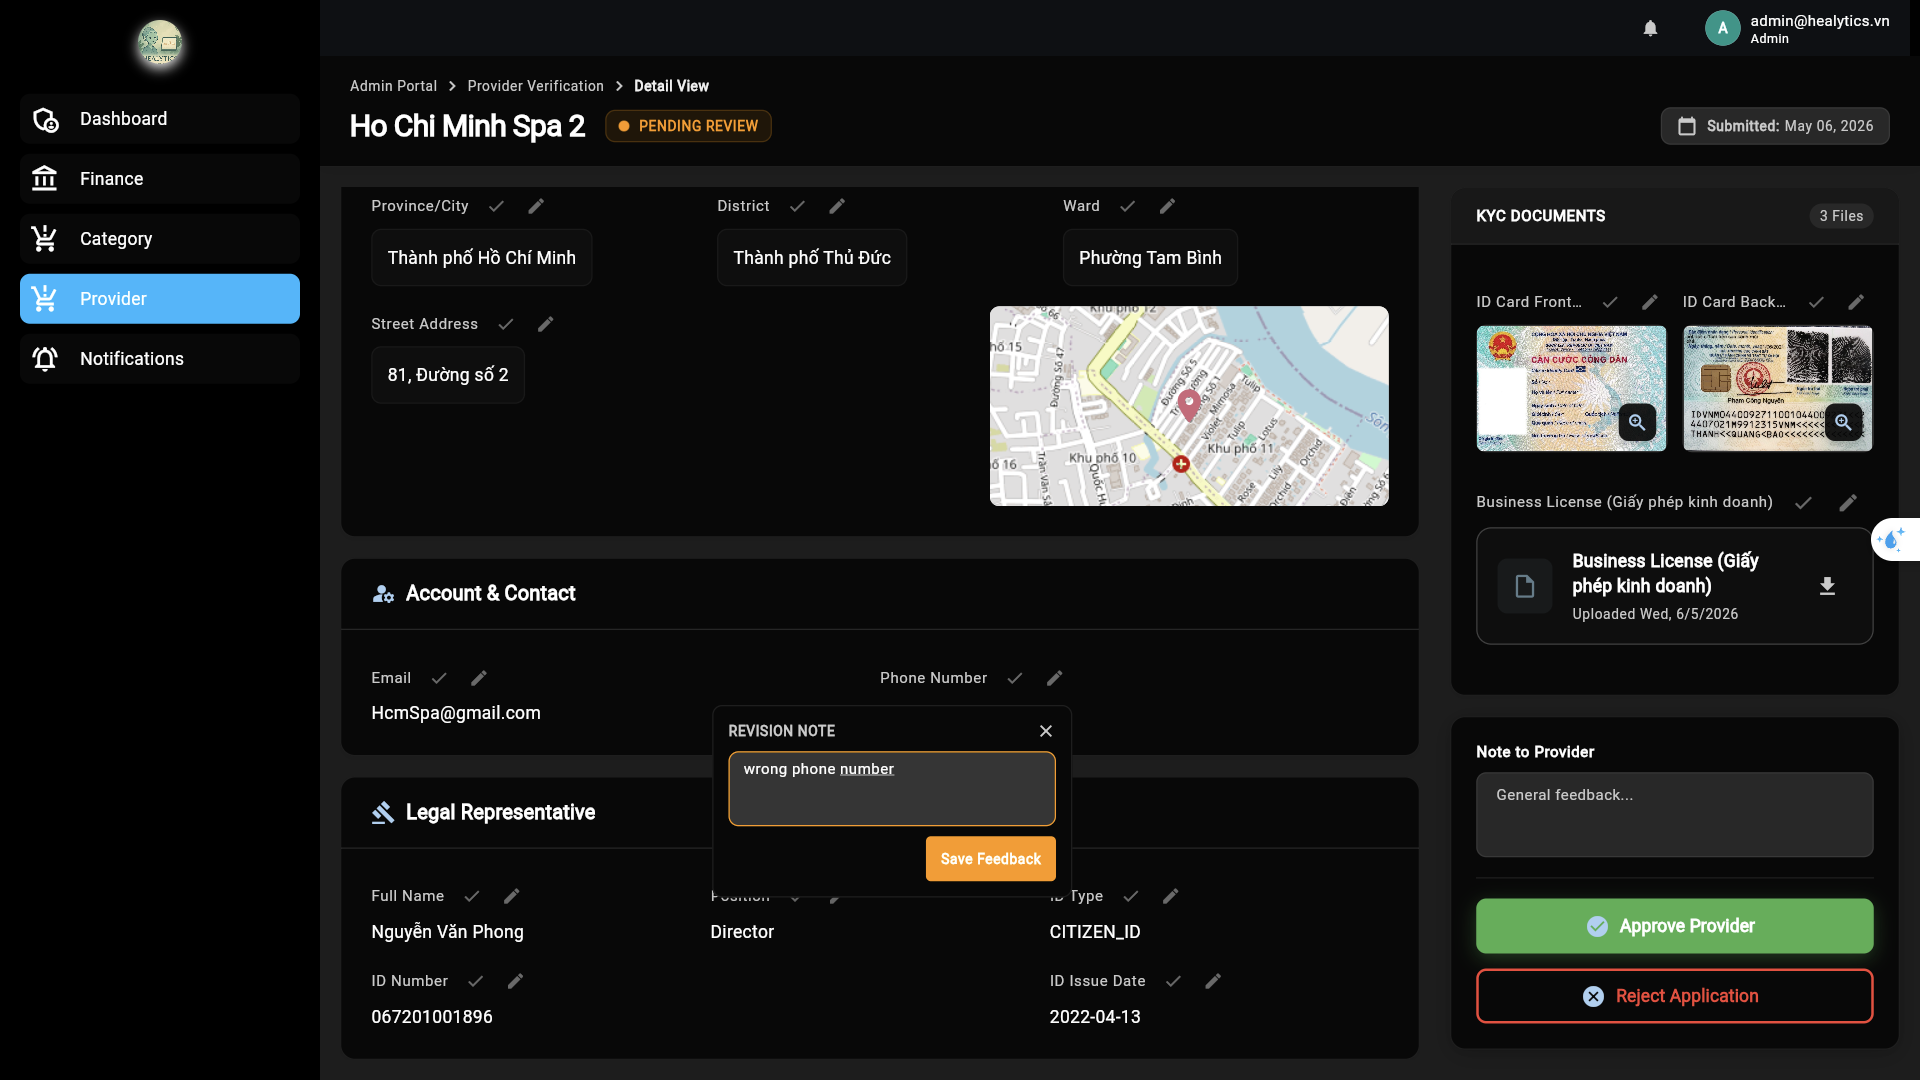
\includegraphics[width=0.92\textwidth]{Images/Hiện thực/admin/fig_admin_provider_revision_note.png}
    \vspace{1em}
    \caption{Popup Revision Note khi đánh dấu trường cần sửa}
    \label{fig:admin_revision_note}
\end{figure}

Hình~\ref{fig:admin_revision_note} hiển thị tính năng ghi chú yêu cầu chỉnh sửa:
\begin{itemize}
    \item \textbf{Popup Revision Note:} Xuất hiện khi quản trị viên nhấn vào biểu tượng bút chỉnh sửa bên cạnh bất kỳ một trường thông tin nào.
    \item \textbf{Nhập lý do:} Quản trị viên nhập phản hồi lỗi cụ thể (ví dụ: ``wrong phone number'') và xác nhận.
    \item \textbf{Hiển thị phản hồi:} Ghi chú này sẽ được đồng bộ và hiển thị trực tiếp trên giao diện của đối tác để hướng dẫn họ cập nhật lại thông tin một cách chính xác.
\end{itemize}

\paragraph{Logic xét duyệt phía Backend}

Khi quản trị viên xét duyệt một hồ sơ đối tác, hệ thống xử lý theo các bước:

\begin{enumerate}
    \item \textbf{Kiểm tra điều kiện:} Chỉ cho phép xét duyệt khi đối tác đang ở trạng thái \texttt{PENDING}. Nếu không, hệ thống trả về lỗi.

    \item \textbf{Phân loại đánh giá:} Quản trị viên gửi danh sách các mục cần đánh giá, mỗi mục gồm \texttt{fieldKey} và \texttt{feedback}. Hệ thống tự động phân loại thành đánh giá trường hồ sơ hoặc đánh giá tài liệu dựa trên danh sách trường đã biết.

    \item \textbf{Lưu ảnh chụp dữ liệu (Snapshot):} Với mỗi mục được đánh giá, hệ thống lưu lại giá trị hiện tại kèm kết quả hợp lệ hay không và phản hồi chi tiết, giúp truy vết chính xác dữ liệu tại thời điểm xét duyệt.

    \item \textbf{Xác định kết quả cuối cùng:} Hệ thống áp dụng quy tắc ưu tiên:
    \begin{itemize}
        \item Nếu quản trị viên chọn từ chối $\rightarrow$ \texttt{REJECTED} (ưu tiên cao nhất, không thể đảo ngược).
        \item Nếu có bất kỳ mục nào bị đánh dấu lỗi $\rightarrow$ \texttt{REQUIRED\_RESUBMIT} (yêu cầu sửa lại).
        \item Nếu tất cả hợp lệ và đủ tài liệu bắt buộc $\rightarrow$ \texttt{APPROVED}.
    \end{itemize}

    \item \textbf{Ghi nhận lịch sử:} Toàn bộ kết quả xét duyệt được lưu vào bảng \texttt{PartnerReviewLog} dưới dạng bản ghi bất biến (immutable), bao gồm: kết quả, người duyệt, nhận xét chung, và chi tiết đánh giá từng trường/tài liệu.
\end{enumerate}

\subsubsection{Quản lý Danh mục và Thông báo}

\paragraph{Module Danh mục (Category)}

\begin{figure}[H]
    \centering
    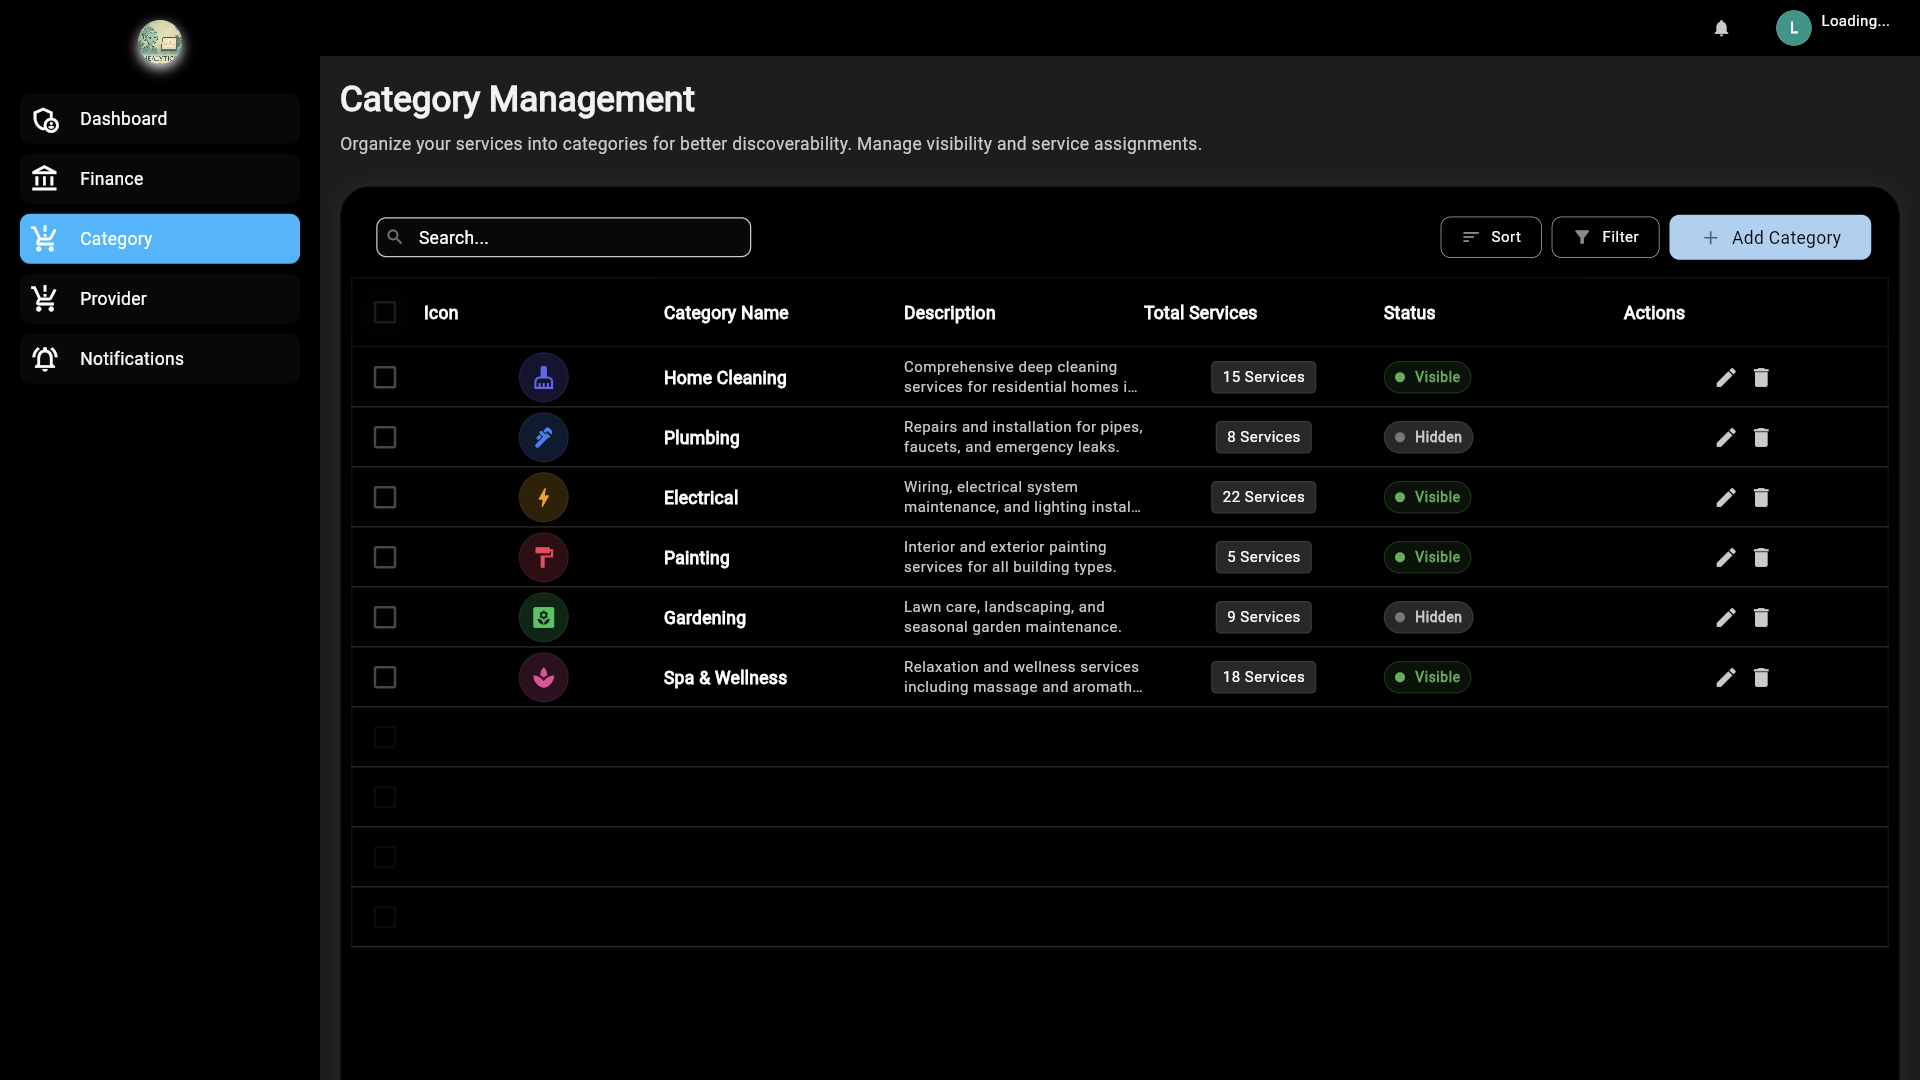
\includegraphics[width=0.92\textwidth]{Images/Hiện thực/admin/fig_admin_category.png}
    \vspace{1em}
    \caption{Giao diện Category Management}
    \label{fig:admin_category}
\end{figure}

Hình~\ref{fig:admin_category} hiển thị giao diện quản lý danh mục dịch vụ:
\begin{itemize}
    \item \textbf{Thông tin hiển thị:} Bao gồm các cột Name, Slug, Icon, Description, Status (Active/Inactive), Services (số lượng dịch vụ đang liên kết), và Created At.
    \item \textbf{Thao tác quản trị:} Cho phép quản trị viên thực hiện tạo mới, chỉnh sửa nội tuyến (inline editing), hoặc chuyển đổi trạng thái hiển thị của từng danh mục.
\end{itemize}

\paragraph{Module Thông báo (Notification Control Center)}

\begin{figure}[H]
    \centering
    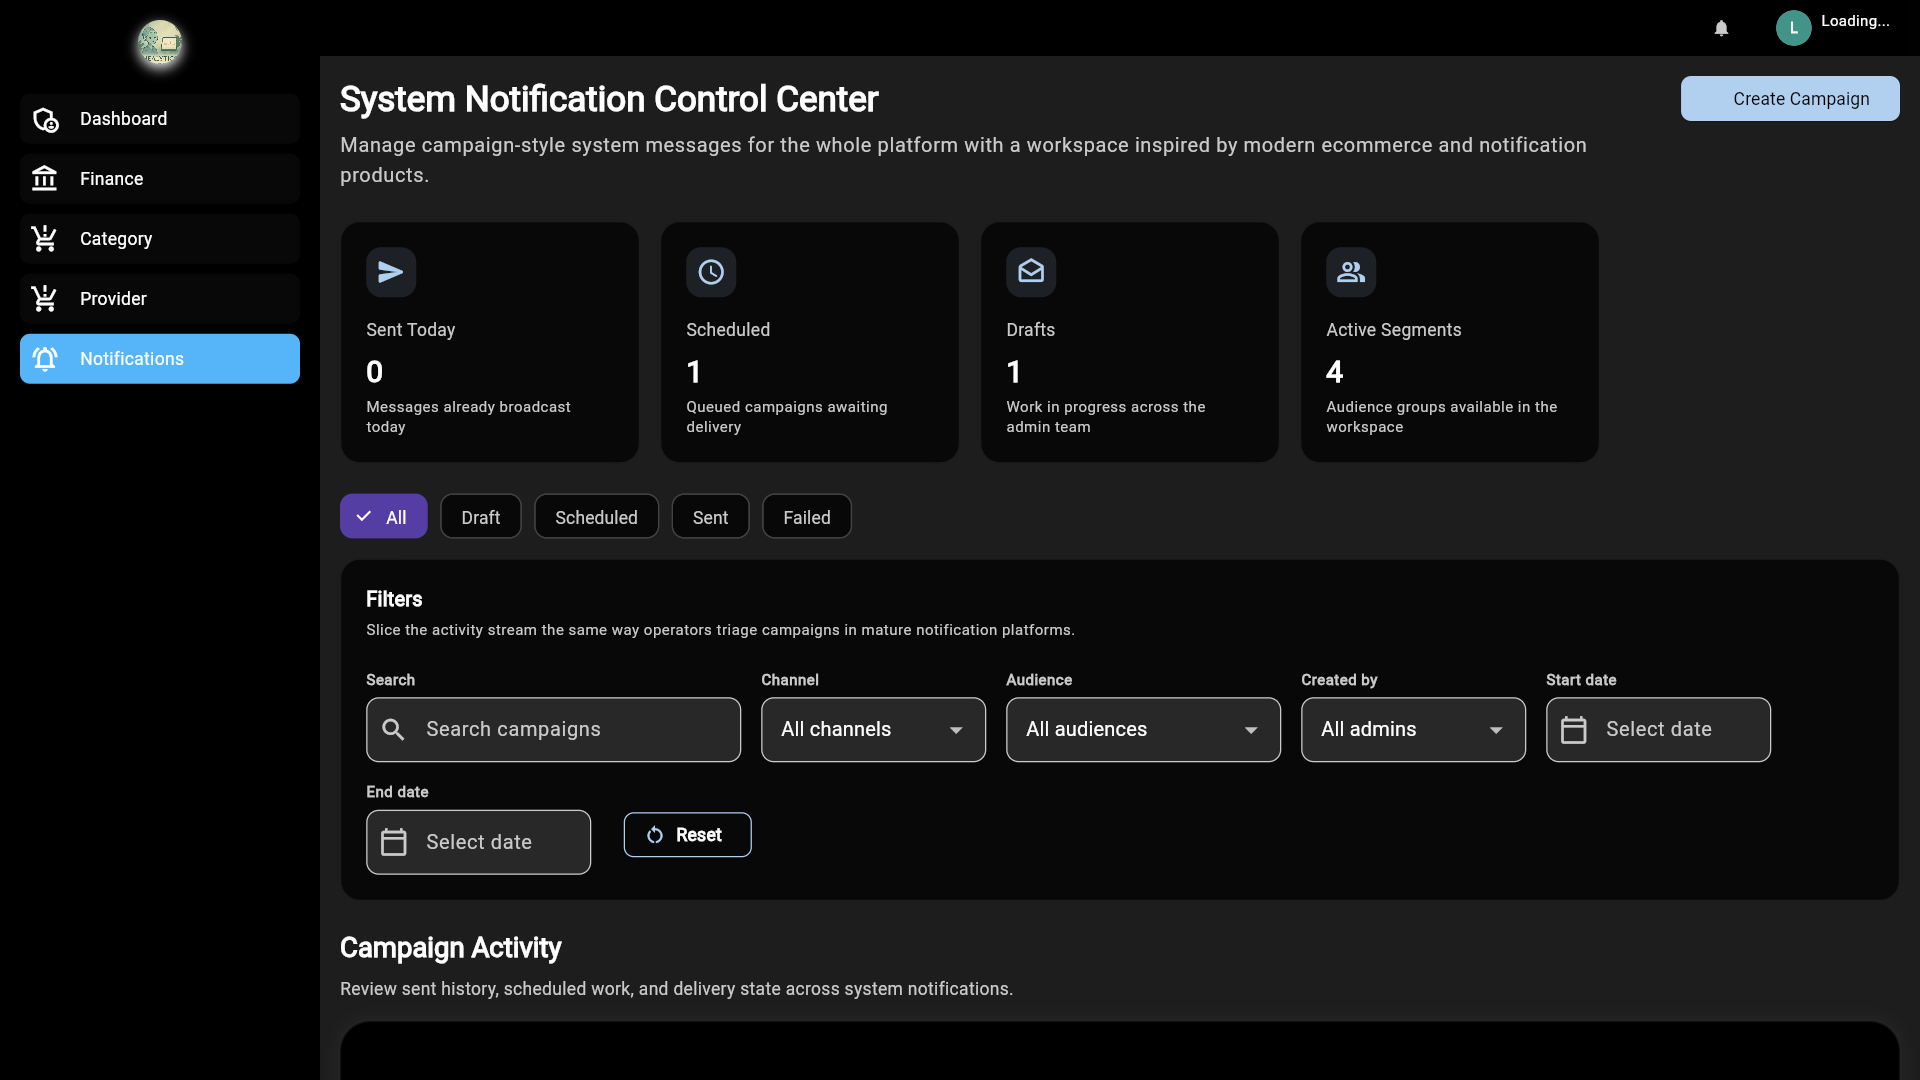
\includegraphics[width=0.92\textwidth]{Images/Hiện thực/admin/fig_admin_notification_center.png}
    \vspace{1em}
    \caption{Giao diện Notification Control Center}
    \label{fig:admin_notification}
\end{figure}

\begin{figure}[H]
    \centering
    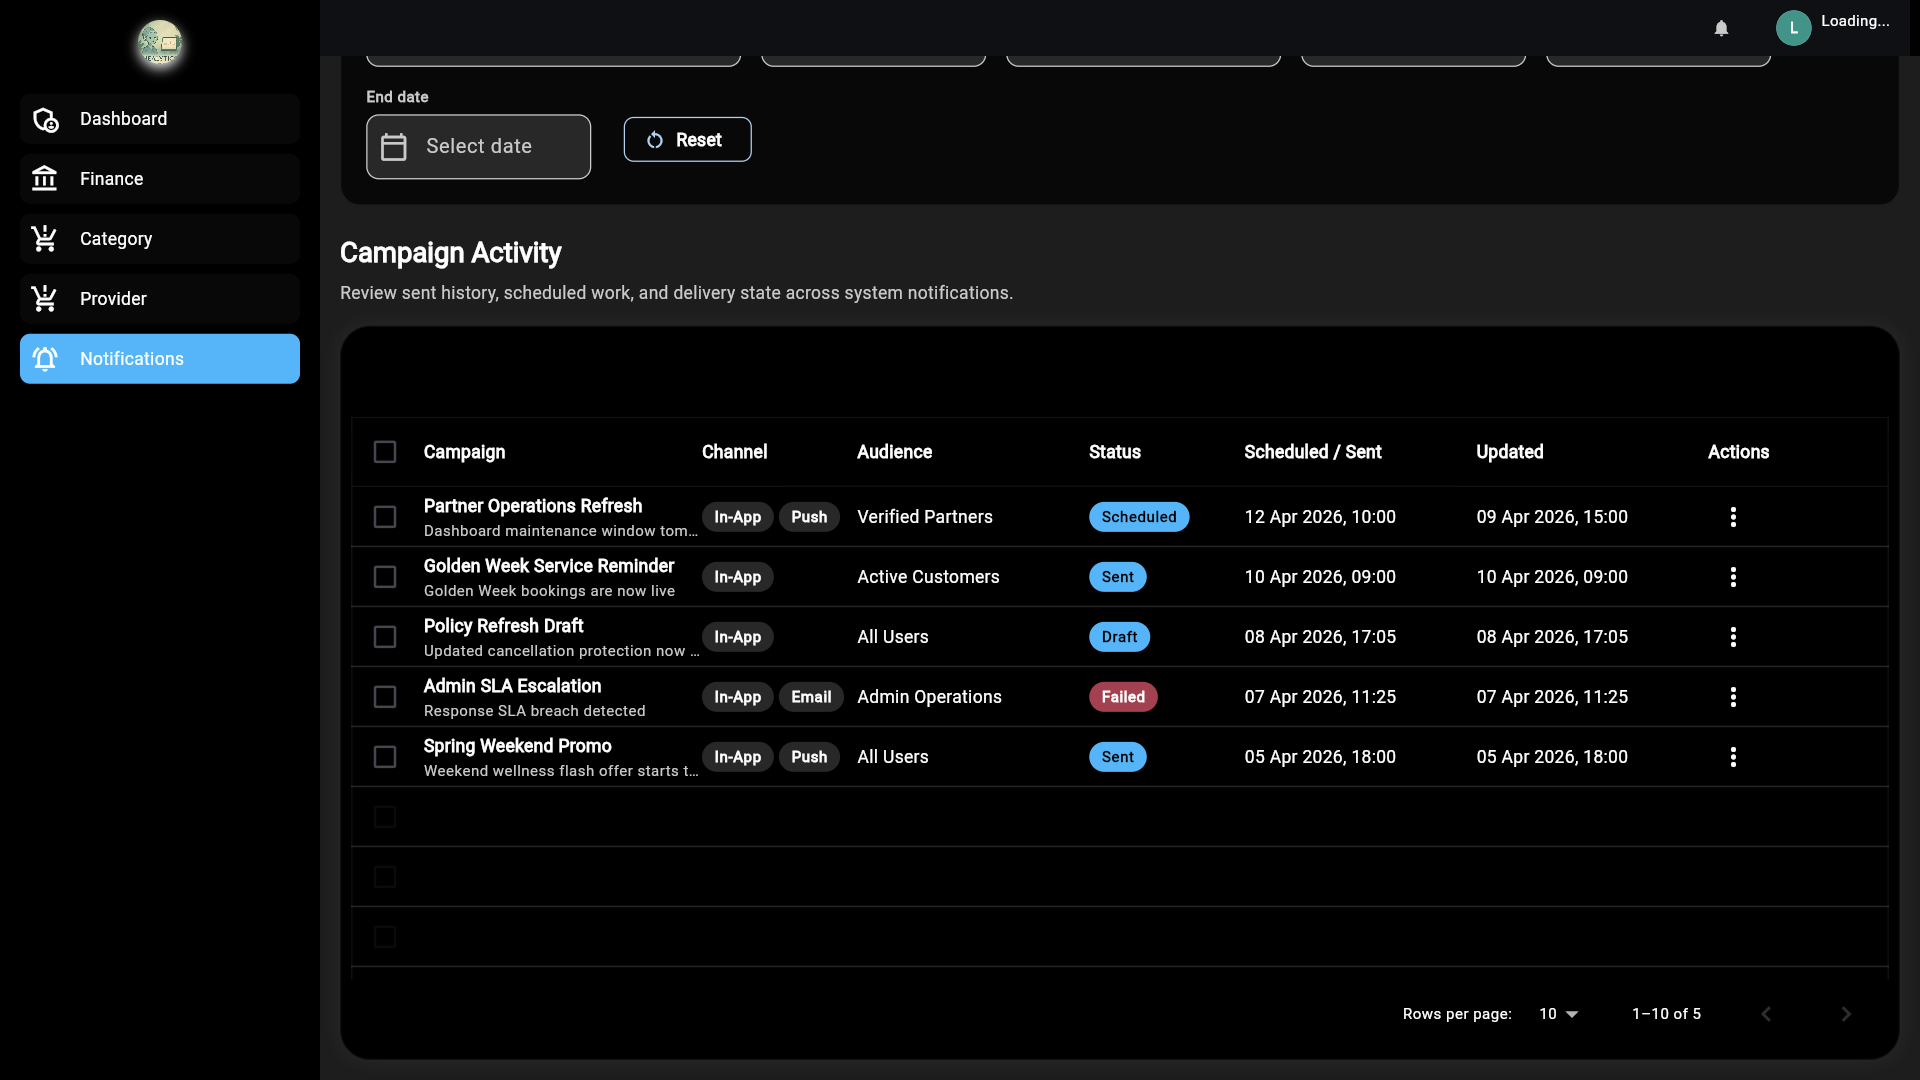
\includegraphics[width=0.92\textwidth]{Images/Hiện thực/admin/fig_admin_notification_campaigns.png}
    \vspace{1em}
    \caption{Notification Control Center -- màn hình quản lý chiến dịch}
    \label{fig:admin_notification_campaigns}
\end{figure}

Hình~\ref{fig:admin_notification} hiển thị Notification Control Center (Trung tâm quản lý thông báo):
\begin{itemize}
    \item \textbf{Tạo chiến dịch:} Cho phép quản trị viên soạn thảo và cấu hình các chiến dịch thông báo broadcast gửi đến những nhóm đối tượng mục tiêu cụ thể.
    \item \textbf{Theo dõi trạng thái:} Cung cấp trạng thái thời gian thực của các thông báo (Draft, Sent, Scheduled, Failed).
    \item \textbf{Phân tích hiệu quả:} Hiển thị các chỉ số tương tác quan trọng như Delivery rates (tỷ lệ gửi thành công), Open rates (tỷ lệ mở), và Click rates (tỷ lệ nhấp chuột).
\end{itemize}

\subsubsection{Nhật ký Kiểm toán (Audit Logging)}

Ngoài lịch sử xét duyệt, hệ thống còn ghi lại mọi thao tác quan trọng của quản trị viên thông qua module \texttt{AuditModule}:

\begin{itemize}
    \item \textbf{Đánh dấu hành động:} Sử dụng decorator \texttt{@Audit} gắn trực tiếp trên các API cần theo dõi, ví dụ: \texttt{@Audit('PARTNER\_REVIEW', 'Partner')}.
    \item \textbf{Tự động ghi nhận:} \texttt{AuditInterceptor} tự động thu thập thông tin trước và sau khi API được thực thi, bao gồm: ai thực hiện, thao tác gì, tác động đến đối tượng nào, và thời điểm cụ thể.
    \item \textbf{Tra cứu linh hoạt:} \texttt{AuditService} cho phép tìm kiếm nhật ký theo người thực hiện, đối tượng bị tác động, hoặc loại hành động.
\end{itemize}

Nhờ kết hợp giữa \texttt{PartnerReviewLog} và \texttt{AuditLog}, hệ thống đảm bảo khả năng truy vết toàn diện: ai đã duyệt hồ sơ nào, vào lúc nào, và dữ liệu lúc đó trông ra sao.



\section{Hiện thực và Tích hợp các dịch vụ Trí tuệ Nhân tạo (AI Services)}
\subsection{Hiện thực dịch vụ nhận dạng thực thể (NER Service)}


\subsubsection{Kiến trúc Hybrid NER và quyết định thiết kế}

Hệ thống dùng kiến trúc \textbf{Hybrid NER}, kết hợp ba lớp xử lý bổ trợ nhau:
\begin{itemize}
    \item \textbf{LLM extraction (Gemini):} xử lý các thực thể ngữ nghĩa trong \texttt{gemini\_ner.py}, với model mặc định \texttt{gemini-2.5-flash}.
    \item \textbf{Rule-based extraction (Regex):} xử lý các mẫu định lượng và làm lớp dự phòng trong \texttt{extractor.py} và \texttt{distance\_extractor.py}.
    \item \textbf{Fallback nội bộ:} kết hợp \texttt{underthesea}, keyword scan và bộ so khớp địa danh (Aho-Corasick hoặc n-gram fallback) trong \texttt{extractor.py}.
\end{itemize}

Các tham số cấu hình chính nằm trong \texttt{config.py}:
\begin{itemize}
    \item \texttt{QUERY\_CACHE\_MAXSIZE = 1000}.
    \item \texttt{LOCATION\_CACHE\_TTL = 3600} giây.
    \item \texttt{GEMINI\_TIMEOUT\_MS = 1500}, \texttt{GEMINI\_MAX\_RETRIES = 1}, \texttt{GEMINI\_COOLDOWN\_SECONDS = 5}.
    \item \texttt{NER\_MIN\_CONFIDENCE = 0.8} cho lọc \texttt{BUSINESS\_TYPE}.
    \item \texttt{DEFAULT\_PROXIMITY\_RADIUS\_M = 10000}, \texttt{MAX\_PROXIMITY\_RADIUS\_M = 50000}.
\end{itemize}


\subsubsection{Pipeline xử lý truy vấn}

Khi nhận truy vấn tự nhiên, NER Service xử lý theo pipeline tuần tự:
\begin{enumerate}
    \item \textbf{Hybrid extraction} (\texttt{extractor.py}): nhận thực thể từ Gemini rồi bổ sung bằng underthesea, keyword và location fallback.
    \item \textbf{Numeric policy} (\texttt{extractor.py}): \texttt{PRICE} và \texttt{DISTANCE} dùng hướng \textit{Gemini-first}; khi Gemini không trả kết quả thì mới rơi về parser cục bộ.
    \item \textbf{Entity normalization} (\texttt{normalizer.py}): quy đổi về schema chuẩn gồm \texttt{business\_type}, \texttt{location\_code}, \texttt{operator}, \texttt{amount}.
    \item \textbf{Spatial resolution} (\texttt{spatial\_context.py}): xử lý ngữ cảnh khoảng cách và tọa độ người dùng.
    \item \textbf{Pre-filter query} (\texttt{query\_builder.py}, \texttt{db\_fetcher.py}): dựng điều kiện truy vấn và lấy ứng viên từ DB/PostGIS.
\end{enumerate}

Đầu ra endpoint:
\begin{itemize}
    \item \texttt{/ner/extract}: trả \texttt{NerResponse} (entities + \texttt{extraction\_source}) trong \texttt{ner\_routes.py}.
    \item \texttt{/prefilter/search}: trả \textbf{List[String]} (danh sách \texttt{service\_id}) trong \texttt{prefilter\_routes.py}.
\end{itemize}

\subsubsection{Tối ưu hiệu năng và độ bền vận hành}

NER Service có một số cơ chế tối ưu quan trọng để giữ độ trễ ổn định trong môi trường thời gian thực:
\begin{itemize}
    \item \textbf{LRU query cache:} giữ tối đa 1000 truy vấn (\texttt{QUERY\_CACHE\_MAXSIZE}) trong \texttt{extractor.py}.
    \item \textbf{Aho-Corasick location matching:} bật/tắt bằng \texttt{LOCATION\_MATCHER\_USE\_AHO}; nếu không khả dụng thì chuyển sang n-gram fallback trong \texttt{extractor.py}.
    \item \textbf{Stale-while-revalidate cho cache địa lý:} TTL 3600 giây trong \texttt{cache.py}.
    \item \textbf{Confidence gating:} ngưỡng \texttt{NER\_MIN\_CONFIDENCE = 0.8} cho \texttt{BUSINESS\_TYPE} trong \texttt{gemini\_ner.py}.
\end{itemize}

\subsubsection{Schema giao tiếp và tính xác định đầu ra}

Dữ liệu trao đổi giữa Gateway và NER Service được chuẩn hóa bằng Pydantic models. Ngoài bộ trường \texttt{type/value/confidence}, mỗi thực thể còn mang thêm thông tin ngữ nghĩa để phục vụ bước dựng truy vấn:
\begin{itemize}
    \item \texttt{business\_type} cho thực thể loại hình dịch vụ.
    \item \texttt{location\_code}, \texttt{location\_level} cho thực thể địa điểm.
    \item \texttt{operator}, \texttt{amount}, \texttt{amount\_max} cho thực thể định lượng.
\end{itemize}

Trong mã hiện thực, schema entity được định nghĩa ở \texttt{ner\_schema.py}. Một ví dụ điển hình là entity \texttt{DISTANCE}:
\begin{itemize}
    \item \texttt{type}: \texttt{"DISTANCE"}
    \item \texttt{value}: chuỗi gốc trong câu hỏi (ví dụ \texttt{"trong bán kính 5km"})
    \item \texttt{confidence}: điểm tin cậy trong đoạn $[0,1]$
    \item \texttt{operator}: \texttt{lte/gte/between}
    \item \texttt{amount}, \texttt{amount\_max}: giá trị số đã chuẩn hóa
    \item \texttt{radius\_meters}: bán kính theo mét để đưa xuống truy vấn không gian
    \item \texttt{distance\_unit}: đơn vị người dùng nhập (\texttt{km}, \texttt{m}, ...)
    \item \texttt{proximity\_intent}: cờ thể hiện ý định tìm gần (tường minh hoặc ngầm định)
\end{itemize}

Các loại entity trong NER Service (theo \texttt{extractor.py}, \texttt{normalizer.py}, \texttt{ner\_schema.py}) gồm:
\begin{itemize}
    \item \texttt{BUSINESS\_TYPE}: loại hình dịch vụ (spa, gym, nha khoa, ...).
    \item \texttt{LOCATION}: địa điểm hành chính (tỉnh/huyện/xã) sau bước chuẩn hóa code.
    \item \texttt{PRICE}: ràng buộc giá, mang \texttt{operator/amount/amount\_max}.
    \item \texttt{DISTANCE}: ràng buộc khoảng cách, mang thêm \texttt{radius\_meters} và \texttt{distance\_unit}.
\end{itemize}

Thiết kế schema như vậy giúp việc chuyển từ ngôn ngữ tự nhiên sang điều kiện SQL/PostGIS rõ ràng hơn, dễ kiểm thử hơn và cũng thuận lợi cho truy vết lỗi trong thực nghiệm.


\subsection{Hiện thực hệ thống RAG Chatbot}

Phần hiện thực mô tả chi tiết cách hệ thống RAG Chatbot được triển khai dựa trên mã nguồn Python mới nhất. Hệ thống được xây dựng theo kiến trúc LangChain pipeline kết hợp FastAPI, hỗ trợ streaming response và tích hợp chặt chẽ với Gateway thông qua cơ chế bất đồng bộ.

\subsubsection{Tiền xử lý, chỉ mục và truy xuất}

Hệ thống được tổ chức theo dạng module hoá rõ ràng, bám sát kiến trúc thiết kế:

\begin{itemize}
    \item \texttt{src/base/llm\_model.py}: Khởi tạo và cấu hình mô hình LLM (quantization 4-bit).
    \item \texttt{src/rag/file\_loader.py}: Load PDF + tiền xử lý + chia đoạn.
    \item \texttt{src/rag/vectorstore.py}: Xây dựng vector database (ChromaDB).
    \item \texttt{src/rag/offline\_rag.py}: Xây dựng pipeline RAG bằng LangChain Runnable.
    \item \texttt{src/rag/main.py}: Kết nối các thành phần thành RAG chain hoàn chỉnh.
    \item \texttt{app.py}: FastAPI app + streaming endpoint.
\end{itemize}

Hệ thống hiện tại ưu tiên sử dụng \textbf{ChromaDB} để đơn giản hóa lưu trữ local và tích hợp trực tiếp với LangChain.

\subsubsection{Hiện thực mô hình ngôn ngữ (LLM)}

Mô hình được load thông qua HuggingFace Transformers với cấu hình lượng tử hoá 4-bit:

\begin{itemize}
    \item Model: \texttt{meta-llama/Llama-3.1-8B-Instruct}
    \item Quantization:
    \begin{itemize}
        \item \texttt{load\_in\_4bit=True}
        \item \texttt{bnb\_4bit\_quant\_type=NF4}
        \item \texttt{double quantization}
        \item compute dtype: float16
    \end{itemize}
    \item max\_new\_tokens: 512
\end{itemize}

Việc sử dụng 4-bit giúp giảm yêu cầu VRAM từ $\sim 24GB \rightarrow 8GB$ mà vẫn giữ chất lượng suy luận chấp nhận được.

LLM được wrap lại bằng \texttt{HuggingFacePipeline} để tích hợp trực tiếp vào LangChain chain.
\subsubsection{Hiện thực xử lý tài liệu và xây dựng vector store}

\paragraph{Load và làm sạch dữ liệu}

Hệ thống sử dụng \texttt{PyPDFLoader} để đọc tài liệu PDF theo từng trang. Sau đó áp dụng hàm:

\begin{itemize}
    \item loại bỏ ký tự không thuộc ASCII (\texttt{ord(char) < 128})
\end{itemize}

Việc này giúp tránh lỗi encoding khi embedding.

\paragraph{Chia đoạn (chunking)}

Sử dụng:
\begin{itemize}
    \item \texttt{RecursiveCharacterTextSplitter}
    \item chunk\_size = 300
    \item chunk\_overlap = 0
\end{itemize}

Khác với thiết kế ban đầu (có overlap), phiên bản hiện tại tối ưu tốc độ và giảm redundancy nên không dùng overlap.

\paragraph{Xây dựng vector store}

Vector DB được khởi tạo thông qua:

\begin{verbatim}
Chroma.from_documents(documents, embedding)
\end{verbatim}

Embedding sử dụng:
\begin{itemize}
    \item \texttt{HuggingFaceEmbeddings}
    \item device ưu tiên CUDA
\end{itemize}

Retriever được tạo bằng:

\begin{verbatim}
retriever = db.as_retriever(
    search_type="similarity",
    search_kwargs={"k": 10}
)
\end{verbatim}

\subsubsection{Hiện thực pipeline RAG bằng LangChain Runnable}

Pipeline RAG được xây dựng theo dạng chain:

\begin{verbatim}
input_data
| prompt
| llm
| output_parser
\end{verbatim}

Trong đó:

\paragraph{Input mapping}

\begin{itemize}
    \item context: question $\rightarrow$ retriever $\rightarrow$ format docs
    \item history: lấy trực tiếp từ request
    \item services: lấy trực tiếp từ Gateway
    \item question: câu hỏi user
\end{itemize}

Cụ thể:

\begin{verbatim}
"context": question → retriever → format_docs
\end{verbatim}

\paragraph{Prompt template (quan trọng)}

Prompt thực tế được thiết kế rất chi tiết với:

\begin{itemize}
    \item phân cấp nguồn tri thức (history → KB → services → LLM)
    \item rule rõ ràng về:
    \begin{itemize}
        \item ngôn ngữ
        \item tone
        \item safety y tế
        \item cách dùng knowledge base
        \item cách dùng services
    \end{itemize}
\end{itemize}

Ví dụ cấu trúc prompt:

\begin{verbatim}
[MEDICAL KNOWLEDGE BASE]
{context}

[CONVERSATION HISTORY]
{history}

[RELEVANT SERVICES]
{services}

[USER QUESTION]
{question}
\end{verbatim}

Điểm quan trọng:
\begin{itemize}
    \item Không ép dùng context nếu không liên quan
    \item Không được hallucinate
    \item Không được chẩn đoán y khoa
\end{itemize}

\paragraph{Output parser}

Custom parser:

\begin{itemize}
    \item loại bỏ prefix như ``Answer:''
    \item chuẩn hoá output về text thuần
\end{itemize}

\subsubsection{Hiện thực Streaming và cơ chế SSE}

\paragraph{Bản chất SSE trong hệ thống}

\textbf{Server-Sent Events (SSE)} là cơ chế cho phép server gửi dữ liệu liên tục về client qua HTTP connection.

\paragraph{Cách hiện thực streaming}

Cụ thể, quá trình được thực hiện theo các bước:

\begin{enumerate}
    \item Mô hình LLM sinh ra từng token một theo câu trả lời.
    \item Nối 3 token liên tiếp thành một chunk.
    \item Các chunk này được phát tuần tự thông qua một \texttt{async generator}, tạo thành luồng dữ liệu liên tục gửi về client.
\end{enumerate}

Cách tiếp cận này đảm bảo:

\begin{itemize}
    \item Trải nghiệm người dùng tương tự streaming token (hiển thị dần nội dung).
    \item Câu trả lời xuất hiện nhanh chóng và liên tục.
    \item Tương thích hoàn toàn với \texttt{StreamingResponse} của FastAPI.
\end{itemize}

Về mặt hiện thực, hệ thống sử dụng cơ chế chia nhỏ văn bản theo cửa sổ trượt. Cơ chế này đóng vai trò là lớp trung gian giữa kết quả sinh hoàn chỉnh của LLM và hệ thống SSE tại Gateway, giúp duy trì trải nghiệm hội thoại thời gian thực mà không làm thay đổi pipeline RAG lõi.


\paragraph{Flow tổng thể SSE}

\begin{enumerate}
    \item Client gửi request
    \item Gateway gọi chatbot service
    \item Chatbot:
    \begin{itemize}
        \item build enriched\_question
        \item gọi RAG chain
        \item Streaming chunk text
    \end{itemize}
    \item Gateway:
    \begin{itemize}
        \item nhận chunk
        \item wrap thành:
        \begin{itemize}
            \item TOKEN
            \item DONE
        \end{itemize}
        \item gửi SSE về client
    \end{itemize}
\end{enumerate}

\subsubsection{Hiện thực endpoint và tích hợp Gateway}

Payload từ Gateway:

\begin{verbatim}
{
    "history": "...",
    "services": "...",
    "question": "..."
}
\end{verbatim}

Chatbot không xử lý intent hay recommendation, mà chỉ:

\begin{itemize}
    \item nhận context đã enrich
    \item sinh câu trả lời
\end{itemize}

Điều này đảm bảo:
\begin{itemize}
    \item tách biệt responsibility
    \item dễ scale microservice
\end{itemize}

\subsubsection{Pipeline tổng hợp cuối cùng}

Pipeline runtime:

\begin{enumerate}
    \item Nhận request từ Gateway
    \item Build enriched input (history + services + question)
    \item Retriever truy xuất context từ Chroma
    \item Build prompt hoàn chỉnh
    \item LLM generate answer
    \item Streaming từng chunk
    \item Gateway convert → SSE → client
\end{enumerate}

Toàn bộ pipeline được thiết kế theo hướng:
\begin{itemize}
    \item tách biệt rõ retrieval vs generation
    \item async-friendly
    \item dễ mở rộng (có thể thay streaming thật sau này)
\end{itemize}



\subsection{Triển khai hệ thống gợi ý}

\subsubsection{Cấu trúc dữ liệu}

Hệ thống được triển khai theo kiến trúc production-ready, trong đó dữ liệu dịch vụ không còn phụ thuộc vào file JSON tĩnh mà được lấy trực tiếp từ cơ sở dữ liệu PostgreSQL. Cụ thể:

\begin{itemize}
    \item \textbf{Services Database}: Bảng \texttt{products} trong PostgreSQL (chỉ lấy các dịch vụ active và hiển thị online)
    \item \textbf{Vector Database}: ChromaDB persistent storage tại \texttt{data/processed/vectordb/}
    \item \textbf{Embedding Model}: \texttt{sentence-transformers/paraphrase-multilingual-mpnet-base-v2}
\end{itemize}

Mỗi service được chuẩn hoá về dạng:

\begin{itemize}
    \item \texttt{service\_id}: định danh duy nhất (ưu tiên \texttt{service\_id}, fallback \texttt{id})
    \item \texttt{name}: tên dịch vụ
    \item \texttt{description}: mô tả
    \item \texttt{category}: phân loại (từ bảng categories)
\end{itemize}

Khác với version ban đầu, các trường như \texttt{tags}, \texttt{type} không còn bắt buộc mà được đơn giản hóa để phù hợp với dữ liệu production.

\subsubsection{Offline Processing}

\paragraph{Document Construction}

Mỗi service được biểu diễn dưới dạng:

\begin{verbatim}
[name] + " " + [description]
\end{verbatim}

Thiết kế này giúp embedding tập trung vào ngữ nghĩa chính thay vì format cứng như trước.

\paragraph{Vector Database Building} 

Quá trình build vector database được thực hiện từ PostgreSQL:

\begin{enumerate}
    \item Query dữ liệu từ bảng \texttt{products} (join với \texttt{categories})
    \item Lọc các service hợp lệ
    \item Tạo document text từ name + description
    \item Embedding thành vector 768 chiều
    \item Upsert vào ChromaDB
\end{enumerate}

Hệ thống hỗ trợ chế độ:

\begin{itemize}
    \item \textbf{clean build}: xoá toàn bộ vector DB và build lại
    \item \textbf{incremental build}: chỉ insert/update các service mới
\end{itemize}

\subsubsection{Đồng bộ dữ liệu thời gian thực}

Hệ thống production triển khai cơ chế \textbf{real-time synchronization} thông qua Redis Pub/Sub.

\paragraph{Cơ chế hoạt động}

\begin{enumerate}
    \item Backend publish event khi có thay đổi dữ liệu:
    \begin{itemize}
        \item \texttt{new\_service\_created}
        \item \texttt{service:updated}
        \item \texttt{service:deleted}
    \end{itemize}
    \item Recommender Service subscribe các channel Redis
    \item Khi nhận event:
    \begin{itemize}
        \item Query lại dữ liệu mới nhất từ PostgreSQL
        \item Re-embedding service
        \item Upsert hoặc delete trong ChromaDB
    \end{itemize}
\end{enumerate}

Cơ chế này đảm bảo:
\begin{itemize}
    \item Không cần rebuild toàn bộ vector DB
    \item Dữ liệu luôn đồng bộ với hệ thống nghiệp vụ
    \item Giảm độ trễ cập nhật xuống gần real-time
\end{itemize}

\subsubsection{Online Processing}

\paragraph{Home Recommender}   

\textbf{Input Format:}
\begin{itemize}
    \item \texttt{user\_id}: Gateway gửi lên, recommender tự truy vấn profile
    \item \texttt{top\_k}: số lượng gợi ý
\end{itemize}

\textbf{Processing Pipeline:}

\begin{enumerate}
    \item \textbf{Fetch User Profile}: lấy health conditions, interests, goals từ database
    \item \textbf{Fetch Service History}: truy vấn các dịch vụ đã sử dụng
    \item \textbf{Query Construction}:
    \begin{itemize}
        \item nối health conditions + interests + goals
        \item bổ sung nội dung dịch vụ đã dùng trước đó
    \end{itemize}
    \item \textbf{Embedding}: chuyển query thành vector
    \item \textbf{Vector Search}: tìm top-k trong ChromaDB
\end{enumerate}

Điểm cải tiến:
\begin{itemize}
    \item Sử dụng trực tiếp document của service history thay vì chỉ ID
    \item Tăng khả năng cá nhân hoá ngữ nghĩa
\end{itemize}

\paragraph{Chatbot Recommender}  

\textbf{Input Format:}
\begin{itemize}
    \item \texttt{query}: câu hỏi tự nhiên
    \item \texttt{conversation\_id}
    \item \texttt{top\_k}
    \item \texttt{filtered\_ids} (optional): danh sách service từ NER
\end{itemize}

\textbf{Processing Pipeline:}

\begin{enumerate}
    \item \textbf{Query Embedding}: chuyển query thành vector
    \item \textbf{Vector Search}:
    \begin{itemize}
        \item Nếu có \texttt{filtered\_ids}:
        \begin{itemize}
            \item áp dụng filter metadata trong ChromaDB
        \end{itemize}
        \item Nếu không:
        \begin{itemize}
            \item search toàn bộ vector space
        \end{itemize}
    \end{itemize}
    \item \textbf{Ranking}: sắp xếp theo cosine similarity
\end{enumerate}

Điểm quan trọng:
\begin{itemize}
    \item Filter được push xuống vector DB (không filter sau khi search)
    \item Giảm search space $\rightarrow$ tăng precision
\end{itemize}

\subsubsection{Tích hợp với Gateway và SSE}

Recommender không trả dữ liệu trực tiếp cho UI mà thông qua Gateway.

\paragraph{Chatbot Flow}

\begin{enumerate}
    \item Gateway nhận message từ user
    \item Gọi song song:
    \begin{itemize}
        \item NER Service
        \item Recommender Service
        \item LLM Service (streaming)
    \end{itemize}
    \item Recommender trả:
    \begin{verbatim}
{
  "service_ids": [...],
  "scores": [...]
}
    \end{verbatim}
    \item Gateway:
    \begin{itemize}
        \item enrich thông tin service từ DB
        \item gửi SSE event:
        \begin{itemize}
            \item \texttt{RECOMMENDATION}
        \end{itemize}
    \end{itemize}
\end{enumerate}

\paragraph{Home Flow}

\begin{itemize}
    \item UI gọi trực tiếp endpoint \texttt{/recommender/home}
    \item Recommender trả danh sách service ID + score
    \item Backend enrich trước khi trả về UI
\end{itemize}

\subsubsection{Đánh giá hiệu năng}

\paragraph{Độ phức tạp}

\begin{itemize}
    \item Embedding: $O(L)$
    \item Vector search: $O(\log N)$ (Chroma internal index)
\end{itemize}

\paragraph{Latency thực tế}

\begin{itemize}
    \item Chatbot recommender: 50–150ms
    \item Home recommender: 80–200ms (do thêm bước fetch profile)
\end{itemize}

\paragraph{Tối ưu}

\begin{itemize}
    \item Upsert thay vì rebuild
    \item Filter ngay tại vector DB
    \item Async processing tại Gateway
\end{itemize}

\subsubsection{Khả năng mở rộng}

Hệ thống được thiết kế theo hướng production:

\begin{itemize}
    \item \textbf{Incremental update}: hỗ trợ upsert từng service
    \item \textbf{Real-time sync}: Redis Pub/Sub
    \item \textbf{Microservice-ready}: tách biệt hoàn toàn với chatbot
    \item \textbf{Hybrid extension}: có thể bổ sung ranking layer phía sau
\end{itemize}

\subsection{Triển khai Intent Classification Model}

\subsubsection{Kiến trúc triển khai}

Trong hệ thống thực tế, Intent Classification được triển khai như một thành phần nhẹ (lightweight component) nằm trực tiếp trong Gateway Service, thay vì tách thành một microservice độc lập. Quyết định này nhằm giảm latency và tránh overhead network call cho một bài toán có độ phức tạp thấp.

Pipeline suy luận bao gồm hai bước tuần tự:

\begin{enumerate}
    \item Mã hoá câu input thành vector embedding
    \item Dự đoán xác suất nhãn bằng mô hình logistic regression
\end{enumerate}

Toàn bộ quá trình xử lý diễn ra đồng bộ (synchronous) và có thời gian thực thi rất nhỏ ($<10ms$), đảm bảo không ảnh hưởng đến luồng xử lý chính của chatbot.

\subsubsection{Quản lý mô hình và khởi tạo}

Mô hình được load theo cơ chế \textbf{singleton} trong vòng đời của ứng dụng:

\begin{itemize}
    \item Encoder (\texttt{SentenceTransformer}) được load một lần khi service khởi động
    \item Classifier (logistic regression) được load từ file pickle
\end{itemize}

Việc sử dụng singleton giúp:

\begin{itemize}
    \item Tránh overhead load model nhiều lần
    \item Giảm độ trễ khi xử lý request
    \item Đảm bảo consistency giữa các lần dự đoán
\end{itemize}

\subsubsection{Tiền xử lý đầu vào}

Câu input từ người dùng được giữ gần như nguyên bản, chỉ thực hiện các bước tối thiểu:

\begin{itemize}
    \item loại bỏ khoảng trắng dư thừa
    \item chuẩn hoá encoding
\end{itemize}

Không áp dụng các kỹ thuật preprocessing phức tạp (stemming, stopword removal) để tránh làm mất thông tin ngữ nghĩa quan trọng cho embedding model.

\subsubsection{Chiến lược dự đoán và ngưỡng quyết định}

Thay vì sử dụng trực tiếp output nhị phân (0/1), hệ thống sử dụng xác suất dự đoán từ logistic regression:

\begin{verbatim}
p = model.predict_proba(embedding)[1]
\end{verbatim}

Sau đó áp dụng một ngưỡng:

\begin{itemize}
    \item $p \geq \theta \rightarrow$ cần gợi ý dịch vụ
    \item $p < \theta \rightarrow$ không cần gợi ý
\end{itemize}

Trong triển khai hiện tại, ngưỡng $\theta$ được tinh chỉnh thực nghiệm (thường trong khoảng 0.5–0.7) để cân bằng giữa:

\begin{itemize}
    \item \textbf{Precision}: tránh gợi ý sai (false positive)
    \item \textbf{Recall}: không bỏ sót nhu cầu thực (false negative)
\end{itemize}

\subsubsection{Tích hợp vào pipeline Gateway}

Intent Classification là bước đầu tiên trong pipeline xử lý hội thoại:

\begin{enumerate}
    \item Nhận message từ user
    \item Phân loại intent
    \item Nếu positive:
    \begin{itemize}
        \item gọi NER Service
        \item gọi Recommender Service
    \end{itemize}
    \item Gọi RAG Chatbot với context đã enrich
\end{enumerate}

Điểm quan trọng:

\begin{itemize}
    \item Intent Classification chạy \textbf{trước tất cả các service khác}
    \item Quyết định trực tiếp việc có kích hoạt recommender hay không
    \item Giúp giảm chi phí compute (không gọi embedding + vector search khi không cần)
\end{itemize}

\subsubsection{Xử lý song song và tối ưu hiệu năng}

Trong trường hợp intent = positive, Gateway triển khai gọi các service theo cơ chế bất đồng bộ:

\begin{itemize}
    \item NER Service
    \item Recommender Service
\end{itemize}

Hai service này được chạy song song (async tasks), sau đó kết quả được tổng hợp trước khi gửi vào RAG.

Intent Classification đóng vai trò như một \textbf{routing gate}, giúp:

\begin{itemize}
    \item giảm số lượng request không cần thiết
    \item tối ưu latency tổng thể của hệ thống
\end{itemize}

\subsubsection{Đánh giá hiệu năng}

\paragraph{Latency}

\begin{itemize}
    \item Encoding (MiniLM): $\sim 5$–8ms
    \item Classification: $<1$ms
    \item Tổng: $<10$ms
\end{itemize}

\paragraph{Memory}

\begin{itemize}
    \item SentenceTransformer: $\sim 80$–120MB
    \item Logistic model: $<1$MB
\end{itemize}

\paragraph{Độ chính xác}

Mô hình đạt độ chính xác tốt trên tập validation nội bộ:

\begin{itemize}
    \item Accuracy: $\sim 85\%$
    \item Precision (positive class): cao hơn recall để giảm false trigger
\end{itemize}

\subsubsection{Khả năng mở rộng}

Thiết kế hiện tại cho phép mở rộng dễ dàng:

\begin{itemize}
    \item Thay thế classifier bằng mô hình deep learning nếu cần
    \item Mở rộng từ binary classification → multi-intent classification
    \item Kết hợp thêm rule-based layer cho các intent đặc biệt
\end{itemize}

Ngoài ra, do component này độc lập với RAG và Recommender, có thể tách thành microservice riêng nếu hệ thống scale lớn hơn.


\section{Triển khai hệ thống (Deployment)}

Toàn bộ hạ tầng hệ thống được container hóa và triển khai tự động thông qua quy trình CI/CD (Continuous Integration / Continuous Deployment) với Jenkins, Docker và Image Registry. Hệ thống được vận hành trên hai môi trường riêng biệt: server CPU (cho Backend và hạ tầng dữ liệu) và server GPU cloud (cho các mô hình AI).

\subsection{Quy trình CI/CD với Jenkins}

Hệ thống triển khai quy trình CI/CD tự động hóa hoàn toàn từ lúc đẩy mã nguồn lên GitHub đến khi cập nhật dịch vụ trên server production. Kiến trúc triển khai được minh họa trong Hình~\ref{fig:deploy_arch}, bao gồm hai thành phần Jenkins chính: \textbf{Jenkins Agent} (chạy trên máy cục bộ) và \textbf{Jenkins Controller} (chạy trên Compute Instance production).

\begin{figure}[H]
    \centering
    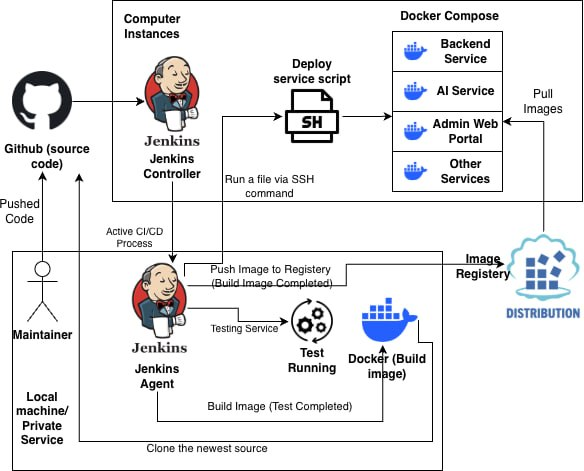
\includegraphics[width=1\textwidth]{Images/Deploy_arch.jpg}
    \vspace{10pt}
    \caption{Kiến trúc triển khai CI/CD của hệ thống}
    \label{fig:deploy_arch}
\end{figure}

\subsubsection{Giai đoạn Build và Test (Jenkins Agent)}

\textbf{Jenkins Agent} được cài đặt trên máy cục bộ (Local Machine / Private Service) của đội ngũ phát triển, chịu trách nhiệm xây dựng và kiểm tra chất lượng mã nguồn trước khi đưa lên production. Quy trình hoạt động như sau:

\begin{enumerate}
    \item \textbf{Clone mã nguồn mới nhất:} Khi Maintainer kích hoạt quy trình CI/CD, Jenkins Agent tự động clone phiên bản mã nguồn mới nhất từ GitHub repository.
    
    \item \textbf{Build Docker Image:} Agent thực hiện build Docker image cho từng service (Backend Service, AI Service, Admin Web Portal, và các service phụ trợ khác) dựa trên Dockerfile tương ứng trong mã nguồn.
    
    \item \textbf{Chạy kiểm thử (Test Running):} Sau khi build thành công, hệ thống tự động chạy bộ test (unit test, integration test) trên Docker image vừa tạo. Chỉ khi toàn bộ test suite pass, quy trình mới tiếp tục sang bước tiếp theo.
    
    \item \textbf{Đẩy Image lên Registry:} Khi test hoàn tất thành công, Jenkins Agent đẩy (push) Docker image đã được kiểm chứng lên \textbf{Image Registry} (Docker Hub hoặc private registry). Mỗi image được gắn tag version tương ứng với commit hash hoặc release version để đảm bảo khả năng truy vết và rollback.
\end{enumerate}

\subsubsection{Giai đoạn Deploy (Jenkins Controller)}

\textbf{Jenkins Controller} được cài đặt trên Compute Instance (máy chủ production), đóng vai trò điều phối việc cập nhật dịch vụ trên môi trường production:

\begin{enumerate}
    \item \textbf{Nhận thông báo từ GitHub:} Khi có mã nguồn mới được đẩy lên GitHub (pushed code), Jenkins Controller nhận webhook trigger và bắt đầu quy trình deploy.
    
    \item \textbf{Thực thi Deploy Script:} Jenkins Controller chạy deploy service script (\texttt{.sh}) thông qua lệnh SSH đến Compute Instance. Script này thực hiện:
    \begin{itemize}
        \item Kéo (pull) các Docker image mới nhất từ Image Registry.
        \item Cập nhật cấu hình Docker Compose nếu cần thiết.
        \item Khởi động lại các service bằng \texttt{docker-compose up -d} với image mới.
    \end{itemize}
    
    \item \textbf{Cập nhật dịch vụ:} Docker Compose trên server production kéo các image mới từ Registry và khởi động lại các container tương ứng, bao gồm:
    \begin{itemize}
        \item \textbf{Backend Service:} NestJS API server.
        \item \textbf{AI Service:} Cụm microservices AI (Gateway, NER, Chatbot, Recommender).
        \item \textbf{Admin Web Portal:} Trang quản trị hệ thống.
        \item \textbf{Other Services:} Các dịch vụ hỗ trợ khác (Kong Gateway, monitoring, v.v.).
    \end{itemize}
\end{enumerate}

\subsubsection{Ưu điểm của kiến trúc CI/CD}

Thiết kế CI/CD hai tầng (Agent--Controller) mang lại nhiều lợi ích:

\begin{itemize}
    \item \textbf{Tách biệt Build và Deploy:} Quá trình build nặng (compile, test) được thực hiện trên máy Agent, không ảnh hưởng đến hiệu năng server production. Server production chỉ cần pull image nhẹ và khởi động lại container.
    
    \item \textbf{Đảm bảo chất lượng:} Mọi thay đổi mã nguồn đều phải qua bước test tự động trước khi được triển khai, giảm thiểu rủi ro lỗi trên production.
    
    \item \textbf{Rollback dễ dàng:} Nhờ việc gắn tag version cho mỗi Docker image trên Registry, hệ thống có thể quay lại phiên bản trước đó nhanh chóng khi phát hiện lỗi.
    
    \item \textbf{Triển khai không gián đoạn (Zero-downtime):} Docker Compose hỗ trợ rolling update, cho phép cập nhật từng service mà không làm gián đoạn toàn bộ hệ thống.
    
    \item \textbf{Tự động hóa hoàn toàn:} Từ lúc developer push code lên GitHub đến khi service mới chạy trên production, toàn bộ quy trình được tự động hóa mà không cần can thiệp thủ công.
\end{itemize}

\subsection{Container hóa với Docker Compose}

File \texttt{docker-compose.yml} tại thư mục \texttt{dockers/} định nghĩa toàn bộ hạ tầng hệ thống, đảm bảo nhất quán giữa môi trường phát triển và production.

\subsubsection{PostgreSQL với PostGIS}

\begin{itemize}
    \item \textbf{Image:} \texttt{postgis/postgis:17-3.5} — PostgreSQL 17 tích hợp PostGIS 3.5 cho truy vấn không gian (tìm dịch vụ gần vị trí người dùng).
    \item \textbf{Khởi tạo:} Script \texttt{init-databases.sh} tự động tạo các database bổ sung cho Kong Gateway và các service phụ.
    \item \textbf{Healthcheck:} \texttt{pg\_isready} kiểm tra trạng thái sẵn sàng trước khi các service phụ thuộc khởi động.
    \item \textbf{Persistence:} Volume \texttt{pgdata} gắn vào \texttt{/var/lib/postgresql/data} giữ dữ liệu khi container restart.
\end{itemize}

\subsubsection{Redis}

\begin{itemize}
    \item \textbf{Image:} \texttt{redis:7-alpine} — phiên bản nhẹ, tối ưu cho container.
    \item \textbf{Persistence:} AOF (Append Only File) kết hợp RDB snapshot (\texttt{--save 20 1}).
    \item \textbf{Bảo mật:} Yêu cầu mật khẩu qua \texttt{--requirepass}, cấu hình từ biến môi trường.
\end{itemize}

\subsubsection{RabbitMQ Cluster (3 nodes + HAProxy)}

Hệ thống triển khai RabbitMQ dạng cluster 3 node đảm bảo tính sẵn sàng cao (High Availability):

\begin{itemize}
    \item \textbf{3 node:} \texttt{rabbitmq1} (primary), \texttt{rabbitmq2}, \texttt{rabbitmq3} tự động join cluster khi khởi động thông qua script \texttt{cluster-entrypoint.sh}.
    \item \textbf{TLS/SSL:} Certificate sinh tự động bởi container \texttt{rabbitmq-cert-gen}, mã hóa giao tiếp giữa các node và client.
    \item \textbf{HAProxy:} Container \texttt{rabbitmq-haproxy} cân bằng tải kết nối AMQP giữa 3 node, đảm bảo failover tự động.
    \item \textbf{Khởi tạo:} Container \texttt{rabbitmq-init} tạo user, vhost và phân quyền cho backend application.
\end{itemize}

\subsection{Kong API Gateway}

Kong đóng vai trò cổng vào duy nhất cho toàn bộ hệ thống, được triển khai gồm 3 thành phần Docker:

\begin{enumerate}
    \item \textbf{Kong Bootstrap (\texttt{kong-bootstrap}):} Container chạy một lần duy nhất để khởi tạo schema database cho Kong trên PostgreSQL.
    \item \textbf{Kong Control Plane (\texttt{kong-cp}):} Instance chính xử lý request. Proxy endpoint tại port 8000, Admin API tại port 8001, Manager UI tại port 8002 cho quản trị trực quan.
    \item \textbf{Kong Configurator (decK):} Sử dụng công cụ \texttt{decK} để đồng bộ cấu hình route, service, plugin từ file \texttt{kong.yml} vào Kong, đảm bảo cấu hình được version control và có thể tái tạo.
\end{enumerate}

Cấu hình route trong \texttt{kong.yml} định tuyến request đến các upstream service tương ứng (NestJS Backend, AI Gateway), đồng thời áp dụng các plugin bảo mật (rate limiting, authentication).

\subsection{Triển khai AI trên RunPod GPU Cloud}

Các mô hình AI yêu cầu GPU mạnh (đặc biệt Llama 3.1 8B với quantization 4-bit) được triển khai trên RunPod — nền tảng GPU cloud theo nhu cầu (on-demand):

\begin{itemize}
    \item \textbf{\texttt{deploy\_runpod.py}:} Script tự động hóa toàn bộ quy trình triển khai: tạo pod GPU trên RunPod, cài đặt môi trường Python và dependencies, tải mô hình từ HuggingFace, và khởi động các AI service (RAG Chatbot, Recommender, NER, Gateway).
    \item \textbf{\texttt{teardown\_runpod.py}:} Script gỡ bỏ pod và giải phóng tài nguyên GPU khi không cần thiết, tiết kiệm chi phí vận hành.
    \item \textbf{Yêu cầu phần cứng:} GPU NVIDIA với tối thiểu 16GB VRAM cho inference Llama 3.1 8B (quantized 4-bit NF4).
\end{itemize}

\subsection{Kiến trúc triển khai tổng thể}

Kiến trúc triển khai tách biệt thành hai cụm độc lập giao tiếp qua REST API:

\begin{itemize}
    \item \textbf{Cụm Backend (Server CPU):} Docker Compose chạy PostgreSQL, Redis, RabbitMQ, Kong và NestJS Backend. Triển khai trên Compute Instance và được cập nhật tự động qua Jenkins Controller.
    \item \textbf{Cụm AI (RunPod GPU):} Các microservices Python (Gateway, NER, Chatbot, Recommender) chạy trên pod GPU cloud. Có thể scale lên/xuống theo nhu cầu thực tế.
    \item \textbf{CI/CD Pipeline:} Jenkins Agent (máy cục bộ) đảm nhận build và test, đẩy image lên Registry. Jenkins Controller (server production) kéo image và triển khai tự động khi có code mới trên GitHub.
    \item \textbf{Kết nối:} Cloudflare Tunnel đảm bảo kết nối an toàn giữa hai cụm và với client bên ngoài.
\end{itemize}

Thiết kế này cho phép scale từng phần linh hoạt: tăng GPU khi lượng truy vấn AI tăng mà không ảnh hưởng đến Backend, hoặc mở rộng Backend khi lượng booking tăng mà không tốn thêm chi phí GPU. Đồng thời, quy trình CI/CD tự động hóa hoàn toàn đảm bảo mọi thay đổi được kiểm thử kỹ lưỡng trước khi lên production, giảm thiểu rủi ro và tăng tốc chu kỳ phát triển.
